\documentclass[11pt, a4paper]{article}
\usepackage[ansinew]{inputenc}
\usepackage[T1]{fontenc}
\usepackage{textcomp}
\usepackage{graphicx}
\usepackage[english]{babel}
\usepackage{hyperref}
%\usepackage{wrapfig}
\usepackage{enumerate}
\usepackage[final]{fixme}
\usepackage{url}
\usepackage{float}
\usepackage{verbatim}
\usepackage{subfig}
\usepackage{pdfpages}
\usepackage{tocvsec2}
\usepackage{setspace}
\usepackage{comment}
\usepackage[numbers]{natbib}
\usepackage{amsmath}
\usepackage{amsfonts}
\usepackage{algorithm}	
\usepackage{algpseudocode}
\usepackage{amsmath}
\usepackage[titletoc,title]{appendix}
\usepackage[dotinlabels]{titletoc}
\usepackage{pgfplots}
\pgfplotsset{compat=1.8}
\usepackage{rotating}
\usepackage[section]{placeins}

\graphicspath{{images/}}

%Allow more page space to be used for figures. From: http://dcwww.camd.dtu.dk/~schiotz/comp/LatexTips/LatexTips.html#figplacement
\renewcommand{\topfraction}{0.85}
\renewcommand{\textfraction}{0.1}
%A figure must use at least 85% of page before it's allowed on a
%single page:

%no widows or orphans
% \widowpenalty=300
% \clubpenalty=300
%allow rubberband values between paragraphs
%\setlength{\parskip}{3ex plus 2ex minus 2ex}


\renewcommand{\floatpagefraction}{0.85}

\newcommand{\FIG}[2]{
\begin{figure}%[!htbp]
  \centering
  \includegraphics[width=0.95\textwidth,keepaspectratio]{#1}
  \caption{#2}
  \label{fig:#1}
\end{figure}
}

\newcommand{\FIGSMALL}[2]{
\begin{figure}%[htbp]
  \centering
  \includegraphics[width=0.4\textwidth,keepaspectratio]{#1}
  \caption{#2}
  \label{fig:#1}
\end{figure}
}

\newcommand{\FIGMED}[2]{
\begin{figure}%[htbp]
  \centering
  \includegraphics[width=0.7\textwidth,keepaspectratio]{#1}
  \caption{#2}
  \label{fig:#1}
\end{figure}
}

\newcommand{\FIGAPP}[2]{
\begin{figure}[htbp]
  \centering
  \includegraphics[height=0.98\textwidth,keepaspectratio,angle=90]{#1}
  \caption{
    #2
  }
  \label{app:#1}
\end{figure}
}

\newcommand{\FIGNOSIZE}[2]{
\begin{figure}[htbp]
  \centering
  \includegraphics{#1}
  \caption{
    #2
  }
  \label{fig:#1}
\end{figure}
}



\newcommand{\FIGH}[2]{
\begin{figure}[H]
  \centering
  \includegraphics[width=0.8\textwidth,keepaspectratio]{#1}
  \caption{#2}
  \label{fig:#1}
\end{figure}
}


%svg importing
\usepackage[]{import}
\usepackage{color}
\newcommand{\executeiffilenewer}[3]{%
  \ifnum\pdfstrcmp{\pdffilemoddate{#1}}%
  {\pdffilemoddate{#2}}>0%
  {\immediate\write18{#3}}\fi%
}
\newcommand{\includesvg}[1]{%
  \executeiffilenewer{#1.svg}{#1.pdf}%
  {inkscape -z -D --file=#1.svg %
    --export-pdf=#1.pdf --export-latex}%
\input{#1.pdf_tex}%
}

\newcommand{\FIGSVG}[2] {
  \begin{figure}[!t]
    \centering
    \def\svgwidth{.4\columnwidth}
    \includesvg{images/#1}
    \caption{#2}
    \label{fig:#1}
  \end{figure}
}


%\bibliographystyle{apalike}
%\bibliographystyle{te}
%\bibliographystyle{plainnat}

\newtheorem{theorem}{Theorem}[section]
\newtheorem{lemma}[theorem]{Lemma}
\newtheorem{proposition}[theorem]{Proposition}
\newtheorem{corollary}[theorem]{Corollary}

\newenvironment{proof}[1][Proof]{\begin{trivlist}
\item[\hskip \labelsep {\bfseries #1}]}{\end{trivlist}}
\newenvironment{definition}[1][Definition]{\begin{trivlist}
\item[\hskip \labelsep {\bfseries #1}]}{\end{trivlist}}
\newenvironment{example}[1][Example]{\begin{trivlist}
\item[\hskip \labelsep {\bfseries #1}]}{\end{trivlist}}
\newenvironment{remark}[1][Remark]{\begin{trivlist}
\item[\hskip \labelsep {\bfseries #1}]}{\end{trivlist}}

\newcommand{\qed}{\nobreak \ifvmode \relax \else
      \ifdim\lastskip<1.5em \hskip-\lastskip
      \hskip1.5em plus0em minus0.5em \fi \nobreak
      \vrule height0.75em width0.5em depth0.25em\fi}
\newcommand{\HRule}{\rule{\linewidth}{0.5mm}}



\begin{document}
\begin{titlepage}
\begin{center}

% Upper part of the page. The '~' is needed because \\
% only works if a paragraph has started.
\textsc{\LARGE Aarhus University}\\[1.5cm]

\textsc{\Large Master Thesis, Computer Science}\\[0.5cm]

% Title
\HRule \\[0.4cm]
{ \huge \bfseries An experimental comparison of max flow algorithms\\[0.4cm] }

\HRule \\[1.5cm]

% Author and supervisor
\begin{minipage}[t]{0.4\textwidth}
\begin{flushleft} \large
\emph{Authors:}\\
Jakob \textsc{Mark Friis} 20080816, jfriis@cs.au.dk\\
\vspace{5mm}
Steffen \textsc{Beier Olesen} 20080991, beier@cs.au.dk\\
\end{flushleft}
\end{minipage}
\begin{minipage}[t]{0.4\textwidth}
\begin{flushright} \large
\emph{Supervisor:} \\
Gerth \textsc{St�lting Brodal}
\end{flushright}
\end{minipage}

\vfill

% Bottom of the page
{\large \today}

\end{center}
\end{titlepage}


\setcounter{tocdepth}{2}
\tableofcontents
\listoffixmes{}

\clearpage

\begin{abstract}
Max flow algorithms have improved a lot since the paper by L. R. Ford and D. R. Fulkerson in 1956 \cite{FordFulkerson}.
The most recent contribution by Orlin \cite{Orlin13} shows that all instances can be solved in $O(nm)$ time.
In this thesis, we will outline the history of max flow problems, as well as implement and compare some of the most interesting ones.
In an effort to improve performance, we managed to reduce the memory used by an algorithm by V. King and S. Rao \cite{King1992} from $O(nm)$ to $O(m)$, 
without compromising the theoretical running time.
\end{abstract}

\clearpage

\section{Introduction}
The max flow problem is a directed graph problem. A graph consists of a set of nodes and a set of edges connecting the nodes.
The edges are directed, meaning that if an edge goes from the node $v_i$ to the node $v_j$, you will be able to follow that edge from $v_i$ to $v_j$, but not the other way.
The graph contains two special nodes, a \emph{source} node $s$ and a \emph{target} node $t$.
The problem is to determine how much flow can be sent through the graph from $s$ to $t$.
Each edge has a limit to the amount of flow that you can send over that edge. 
This limit is called the capacity of the edge, and that is what limits how much flow that you can send from $s$ to $t$.
In the end of any max flow algorithm, there is not allowed to be any flow imbalance in nodes other than $s$ and $t$.
That means that for any node other than $s$ and $t$, the total amount of incoming flow has to be equal to the total amount of outgoing flow.
An example can be seen in Figure~\ref{maxFlowExample}. The numbers on the edges in the first graph signify the capacity of the edges.
The numbers in the solution graph signify how much flow is sent on the edge out of the capacity on the edge.
\begin{figure}[ht!]
\centering
\includegraphics[width=90mm]{MaxFlowExample.png}
\caption{An example of a max flow problem and a solution to it}
\label{maxFlowExample}
\end{figure}

A number of problems can be reduced to the max flow problem, such as maximum cardinality bipartite matching, maximum independent path and maximum edge-disjoint path.
Maximum cardinality bipartite matching problem is, given a bipartite undirected graph with node sets $U$ and $V$, 
select the maximum number of edges connecting $u\in U$ and $v \in V$ such that no nodes are connected to two selected edges.
An example of using max flow to solve maximum cardinality bipartite matching can be seen in Figure~\ref{maxCardinalityBipartiteMatchingExample}.
\begin{figure}[ht!]
\centering
\includegraphics[width=90mm]{MaxCardinalityBipartitMatchingExample.png}
\caption{A max flow solution to maximum cardinality bipartite matching}
\label{maxCardinalityBipartiteMatchingExample}
\end{figure}



An area where real world max flow problems arise is in computer vision. 
The problem of identifying objects in an image can be reduced to a min-cut problem, which is the dual of the max flow problem.
Min cut being the dual of the max flow means that solutions to one of the problems can easily be transformed into a solution to the other.
Furthermore, making a cut in the graph gives an upper bound to the solution while a valid flow in the graph is a lower bound on the solution.

Max flow algorithms have been around since 1956 \cite{FordFulkerson}, and since then many interesting algorithms have been published in the field.
A recent publication by Orlin \cite{Orlin13} proved that max flow problems can be solved in $O(nm)$ time for sparse graphs where $m=O(n^{16/15-\varepsilon})$.
Combined with a result by V. King and S. Rao \cite{King1992}, this means that we have an $O(nm)$ time algorithm for all max flow problems.

Many of the max flow algorithms focus on providing theoretical improvements, and have little to no focus on practical running time.
In this thesis, we will compare the practical running time on a selected subset of the max flow algorithms.
We have decided only to consider max flow problems with integer capacities. The reason for this is that it makes it simpler to implement the algorithms if we don't have to take floating point errors into account.
With integer capacities, all correct implementations are guaranteed to return exactly the same output, which makes it easier to verify.

We start by going over the terminology that we will use throughout the thesis in Section~\ref{TerminologySection}.
Some central ideas are repeated throughout several papers. We give a general overview of these ideas in Section~\ref{ParadigmsSection}.
Section~\ref{SurveySection} will contain a survey where we give a brief overview of the main improvements made since the first paper in the field \cite{FordFulkerson}.
Sections~\ref{EK1972Section} to~\ref{GRSection} contain more detailed descriptions of the algorithms we selected to study. 
We explain how the algorithms work, how they achieve their bounds, and what, if any, modifications we have done to implement them.
Sections~\ref{TestsSection} and~\ref{ResultsSection} contain a description of the tests we have run, and the results we have obtained.

\section{Terminology}
\label{TerminologySection}

We use $G=(V, E)$ to symbolise the graph that we are running the max flow algorithms on.
Here $V$ is a set of nodes, $E$ is a set of edges, and $(u, v)\in E$ is a directed edge where $u\in V$, $v \in V$ and $u \not= v$.
We use $n$ and $m$ to symbolise the number of nodes and the number of edges in the graph, respectively.
If $(u, v)$ exists in $E$, we assume that $(v, u)$ also exists in $E$.
With the max flow problem, two nodes, \emph{source} and \emph{target} are given. We denote them by $s$ and $t$ respectively.

We assume without loss of generality that all nodes can be reached from the source, and that all nodes can reach the target. 
Graphs that do not satisfy this assumption can be trimmed to fit the constraint in $O(m)$ time by performing breadth first searches from the source and from the target.

A \emph{path} in a graph is defined as a list of nodes $(v_1, \ldots , v_k)$ where \\
$(v_i, v_{i+1}) \in E$ for $i=1, \ldots, k-1$ and the list contains no duplicates.

Every edge $(u, v)$ has a \emph{capacity} associated with it denoted by $cap(u, v)$. The capacity of an edge must be a non-negative integer. This is an upper bound on the amount of flow we are allowed to send on the edge.
We use $U$ to represent the maximum capacity over all edges in the graph.
The actual \emph{flow} sent on an edge is denoted by $f(u, v)$. As with capacity, the flow on an edge must be a non negative integer. 
\emph{Residual capacity} on an edge is the amount of flow that can still be sent on the edge without violating the capacity constraint.
It is defined as $r(u, v) = cap(u, v) - f(u, v) + f(v, u)$. For edges $(u, v)\not\in E$, we define $cap(u, v)=f(u, v)=r(u, v)=0$.
An edge $(u, v)$ is said to be \emph{saturated} if $r(u, v) = 0$, and the act of saturating an edge is changing the flow to make the edge become saturated.

A path $P=(v_1, \ldots , v_k)$ is said to be \emph{residual} if $r(v_i, v_{i+1}) > 0$ for $i=1, \ldots, k-1$.
An \emph{augmenting path} $P=(v_1, \ldots , v_k)$ is a residual path in $G$ where $v_1 = s$ and $v_k = t$.
In other words, an augmenting path is a path from $s$ to $t$ in the residual network, where it is possible to send more flow.
The \emph{bounding edges} of an augmenting path is the edges that have the minimum residual capacity of all edges in the path.
As a consequence, if additional flow equal to the minimum residual capacity was pushed on the path, these edges would become saturated.

The \emph{distance} between two nodes $u$ and $v$ is denoted $distance(u, v)$, and is the number of edges connecting nodes in the shortest residual path connecting the two nodes.
If no such path exists, $distance(u, v)=n$. 
This could be infinity instead of $n$, but since the longest path possible contain all nodes, there can at most be $n-1$ edges in such a path.
Infinity can not be represented in a traditional integer, so $n$ is easier to work with.


The \emph{excess} of a node $v$, $e(v)$ is how much flow has been sent to the node, but not sent on to other nodes. It is defined as $e(v)=\sum_{u \in V}\left(f(u, v) - f(v, u)\right)$. 
This may generally only be negative for the node $s$ and positive for the node $t$ and 0 for all other nodes.


In order to have a valid flow, the following conditions must be met:
\begin{enumerate}
  \item  $\forall v \in V \setminus \{s, t\}, e(v) = 0$ 
  \item $\forall (u, v) \in E , f(u, v) \leq cap(u, v)$
\end{enumerate}
The first is referred to as the flow conservation constraint, and the second is the capacity constraint.
Some algorithms works by manipulating \emph{preflow}, which is a flow in the graph where the excess of nodes are allowed to be positive, thus violating the flow conservation constraint.

Tables of all definitions used throughout the thesis can be found in Appendix~\ref{TerminologyAppendix}.

\section{Paradigms}
\label{ParadigmsSection}

There are three general ideas that repeat throughout the max flow algorithms in the literature.


\subsection{Augmenting Paths}
The first idea was introduced by L. R. Ford and D. R. Fulkerson in 1956 \cite{FordFulkerson}, and consists of finding augmenting paths in the graph.
The basic idea is that if you repeatedly find and saturate all augmenting paths in the graph, no more flow can be sent from $s$ to $t$, and you must have a max flow.

The number of augmenting paths an algorithm finds depends on the order in which augmenting paths are found. 
For instance if you consider the graph in Figure~\ref{augmentingPathsExample}, an augmenting path can be made with minimum residual capacity $1$.
Following that path, another can be found with residual capacity $1$ if you follow the middle edge in the opposite direction.
So on this graph, anywhere from $2$ to $1000$ augmenting paths can be found.
\begin{figure}[ht!]
\centering
\includegraphics{augmentingPathsExample.png}
\caption{}
\label{augmentingPathsExample}
\end{figure}
If we didn't have integer capacities, graphs can be created for which infinity many augmenting paths could be found if they are found in a special order.

The idea that no more flow can be sent if no augmenting path can be found is also what is often used to prove correctness of a max flow algorithm. 
If the flow is valid, and there is no augmenting paths in the residual graph, you must have found the max flow.

The algorithm explained in Section~\ref{EK1972Section} is based on finding augmenting paths.

\subsection{Blocking Flow}

The \emph{blocking flow} idea was introduced by E. A. Dinic in 1970 \cite{dinic1970}.
The idea is to construct a \emph{layer graph} that only contains the edges that increase the distance from $s$.
The nodes in the layer graph are the same as the nodes in the graph $G$,
and an edge $(u, v)$ only exists in the layer graph if $distance(s, u) < distance(s, v)$, and $r(u, v) > 0$.
In most blocking flow algorithms, it is sufficient that the layer graph is a directed acyclic graph (DAG).
The general idea is that all paths from $s$ to $t$ have the same length, so you can find the augmenting paths shortest to longest,
but algorithms like Goldberg Rao \cite{Goldberg1998} actually might add some edges $(u, v)$ to the graph where $distance(s, u) = distance(s, v)$,
as long as the graph remains acyclic.

The interesting thing about the layer graph is that it contains all augmenting paths of a certain length $k$, where $k$ is the length of the shortest augmenting path in the residual network of $G$.
The algorithm can now find the max flow in this smaller layer graph. This flow is denoted the \emph{blocking flow}.
Most blocking flow algorithms then continue by updating the residual network of the original graph with the blocking flow, and calculating a new layer graph, which will have a bigger $k$.
This process repeats until all augmenting paths have been found.

\begin{figure}[!ht]
\centering
\includegraphics[width=120mm]{dinicExample.png}
\caption{An example of running a blocking flow algorithm.}
\label{dinicExample}
\end{figure}

The algorithm explained in Section~\ref{DinicSection} is an example of a blocking flow algorithm.
For an example of running a blocking flow algorithm, see Figure~\ref{dinicExample}.


\subsection{Push Relabel}

The \emph{push relabel} idea was introduced by A. V. Goldberg and R. E. Tarjan in 1988 \cite{Goldberg1988}.
This idea differs substantially from the previous two ideas, in that it does not explicitly find augmenting paths.
Instead it works by manipulating a preflow in the algorithm, by violating the flow conservation constraint throughout the algorithm, and pushing excess between individual nodes by adding flow on the edges in the graph.

The idea is to assign a non-negative integer \emph{label} $d(v)$ to each node. 
It starts with giving $s$ the label $n$, and all other nodes the label $0$. 
It then pushes as much flow as possible from $s$ to the neighbours of $s$. The main part of the algorithm is a sequence of pushes and relabels. 
A relabel on a node increases its label by at least one. 
A push sends flow from one node $u$ to another node $v$, but this is only allowed if $d(u) > d(v)$. 
Apart from in the initialization, the nodes $s$ and $t$ are never relabelled, and are never the source of a push.

A relabel should only be performed if a node has some excess, but no place to send it. 
If a node receives excess, it can always send it back to the node it received it from, so if it has no place to send its excess, there must be some neighbour with a higher label, where the excess can be sent.

What is going to happen when running a push relabel algorithm is a sequence of pushes and relabels that move excess around the graph from node to node.
At some point, the nodes will start to be relabelled above $n$. 
When this happens, $t$ is no longer reachable.
A result of having labels above $n$ is that excess will  begin to be pushed back towards $s$. 
Eventually, all the excess will have been pushed to either $s$ or $t$, which means that the flow conversation constraint is fulfilled. 
At this point, a push relabel algorithm will have found a valid flow, which is in fact the max flow.

\begin{figure}[!ht]
\centering
\includegraphics[width=120mm]{pushRelabelExample.png}
\caption{An example of running a push relabel algorithm.}
\label{pushRelabelExample}
\end{figure}

An example of running a push relabel algorithm can be seen in Figure~\ref{pushRelabelExample}.
See Section~\ref{GoldbergTarjanSection} for details on a concrete push relabel algorithm.

\section{Dynamic Trees} \label{Dynamic Trees}

Dynamic trees, also called link cut Trees, is a data structure that was presented by D. D. Sleator and R. E. Tarjan in 1983 \cite{sleator1983}.
It is a forest where each node in a tree can maintain set of values assigned to them, such as a cost.
Updates done to the tree are performed in amortized $O(\log k)$ time, where $k$ is the size of the tree the update is performed on.
The operations supported by dynamic trees are

\begin{description}
  \item[Link($a$, $b$)] \hfill \\
  Make $a$ a child of $b$. $a$ has to be a root for this to be possible.
  \item[Cut($a$)] \hfill \\
  Remove the edge from $a$ to its parent, making $a$ a root node in its own tree.
  \item[SetCost($a$, $c$)] \hfill \\
  Set the cost of $a$ to $c$.
  \item[GetCost($a$)] \hfill \\
  Returns the cost of $a$.
  \item[AddCost($a$, $c$)] \hfill \\
  Modify the cost of $a$ and all of its ancestors by adding $c$.
  \item[GetPathLength($a$)] \hfill \\
  Returns the number of nodes on the path from $a$ to the root of the tree $a$ is in.
  \item[GetRoot($a$)] \hfill \\
  Returns the root of the tree $a$ is in.
  \item[GetChildren($a$)] \hfill \\
  Returns the children of $a$.
  \item[GetMinCostNode($a$)] \hfill \\
  Returns the last node on the path from $a$ to the root of the tree that has the minimum cost of all the nodes on the path.
  \item[GetBoundingNode($a$, $c$)] \hfill \\
  Returns the first node on the path from $a$ to the root of the tree that has a cost less than or equal to $c$.
\end{description}

In max flow algorithms, a dynamic forest is typically used to represent paths of nodes in a way such that each node in the graph has a corresponding node in the dynamic forest.
The nodes in the graph will have an edge which is the preferred edge to move flow along. Linking $a$ to $b$ represents that the edge $(a, b)$ is the preferred edge of $a$.
The cost of the nodes in the dynamic forest will represent the residual capacity on the preferred edge.
This way, a \emph{Tree~Push} can be performed, where moving flow along a path can be done in $O(\log n)$ time instead of $O(n)$ time.
The specifics of how this is done depends on the max flow algorithm, the way it is done for Goldberg Tarjan in Section~\ref{GoldbergTarjanSection} is
\begin{align*}
&v_j \gets \mathrm{GetMinCostNode}(v_i)\\
&c \gets \mathrm{GetCost}(v_j)\\
& \mathrm{AddCost}(v_i, -c)\\
& \text{Cut all GetMinCostNodes with 0 cost}
\end{align*} 
Since the dynamic tree can update the residual capacity of $k$ edges in $\log k$ time, it is not possible to keep a value updated in the graph.
For this reason, algorithms will have an incorrect residual capacities in the graph while an edge or its corresponding back edge is in the dynamic tree. 
The residual capacities are instead updated when a node is cut from the tree.

\clearpage
\section{Survey}
\label{SurveySection}

The purpose of this survey is to give an overview of the most important papers about solving the max flow problem.
For the algorithms presented, we give a short introduction to the main ideas and techniques used, 
but for the details we direct the reader to the original articles.\\\\
\makebox[\textwidth][c]{
\begin{tabular}{ l l l l }
Year & Authors & Running Time & Ref \\
\hline 
1956 & Ford, Fulkerson & $O(nmU)$ & \cite{FordFulkerson} \\
1970 & Dinic & $O(n^2m)$ & \cite{dinic1970} \\
1972 & Edmonds, Karp & $O(nm^2)$ & \cite{Edmonds1972} \\
1974 & Karzanov & $O(n^3)$ & \cite{karzanov1974} \\
1977 & Cherkasky & $O(n^2\sqrt{m})$ & \cite{Che77} \\
1978 & Malhotra, Kumar, & $O(n^3)$  & \cite{MKM78} \\
     & Maheshwari \\
1979 & Gali, Naamad & $O(nm\log^2n)$ & \cite{Galil1979}\\
1980 & Gali & $O(n^\frac{5}{3}m^\frac{2}{3})$ & \cite{Galil1980} \\
1983 & Sleator, Tarjan & $O(nm\log n)$ & \cite{sleator1983} \\
1984 & Tarjan & $O(n^3)$ & \cite{Tarjan1984} \\
1985 & Gabow & $O(nm\log U)$ & \cite{Gabow1985} \\
1988 & Goldberg, Tarjan & $O(nm\log{\frac{n^2}{m}})$ & \cite{Goldberg1988} \\
1989 & Auija, Orlin & $O(nm+n^2\log{U})$ & \cite{AO1989} \\
1989 & Auija, Orlin, Tarjan & $O(nm\log{\left(\frac{n}{m}\sqrt{{\log{U}}}+2\right)})$ & \cite{AOT1989} \\
1989 & Cheriyan, Hagerup & 
$E\left(\min{\left(
\begin{aligned}
&nm\log{n}\\
&nm+n^2\log^2{n}
\end{aligned}
\right)}\right)$ & \cite{Cheriyan1989} \\
1990 & Alon & $O(\min{\{nm\log{n},n^{\frac{8}{3}}\log{n}\}})$ & \cite{Alon1990} \\
1992 & King, Rao & $O(nm + n^{2+\varepsilon})$ & \cite{King1992} \\
1994 & King, Rao, Tarjan & $O(nm\log_{\frac{m}{n}\log{n}}{n})$ & \cite{King1994} \\
1998 & Goldberg, Rao & $O(\min{\{n^{\frac{2}{3}},\sqrt{m}\}}m\log{(\frac{n^2}{m})}\log{U})$ & \cite{Goldberg1998} \\
2012 & Orlin & $O(nm + m^{31/16}\log^2{n})$ & \cite{Orlin13} \\
\hline \\
\end{tabular}
}

The first algorithm for solving the max flow problem was introduced in 1956 by L. R. Ford and D. R. Fulkerson \cite{FordFulkerson}. 
They proposed an algorithm that iteratively finds augmenting paths. 
Since they posed no restrictions on the order with which paths are found, their algorithm runs in $O(nmU)$ for integer capacity constraints.
This bound is achieved by observing that $nU$ is an upper bound on the flow that can be sent, since there can be $n$ edges out of $s$, and each of them has at most $U$ capacity.
Each augmenting path sends at least $1$ unit of flow, so this results in $O(nU)$ augmenting paths. Finding an augmenting path can be done in $O(m)$ time, which leads to the bound of $O(nmU)$. 
It is not guaranteed to terminate on real valued constraints.
In 1972, J. Edmonds and R. M. Karp \cite{Edmonds1972} observed that if the augmenting path found in the algorithm by Ford and Fulkerson always is a shortest augmenting path, the maximum number of augmenting paths is $O(nm)$.
This algorithm runs in $O(nm^2)$ time. We explain this algorithm in more detail in Section~\ref{EK1972Section}.

About the same time, in 1970, E. A. Dinic \cite{dinic1970} published another improvement over the algorithm by Ford and Fulkerson.
The paper by Dinic also includes the algorithm by Edmonds and Karp, but Dinic includes additional techniques to reduce the running time to $O(n^2m)$.
His idea was to remove some edges in the graph, to get a layer graph which contain all paths from $s$ to $t$ that have length $k$, where $k$ is the length of the shortest augmenting path in $G$. 
He then finds all augmenting paths in this layer graph, which is called the blocking flow. 
After that, he calculates the residual network of the original graph augmented with the blocking flow. With this new residual network, he finds a new layer graph where $k'>k$.
To find all paths in the layer graph, he used a depth first search. 
Many subsequent algorithms are based on this idea of using layer graphs, but have an optimized algorithm for finding the blocking flow.
More details on this algorithm can be found in Section~\ref{DinicSection}.

The first optimization to Dinic's algorithm was published by A. V. Karzanov in 1974 \cite{karzanov1974}. He came up with a very complicated algorithm for finding the blocking flow that uses preflows.
This algorithm reduced the running time to $O(n^3)$, which is $O(nm)$ for very dense graphs where $m=\Theta(n^2)$.
There have been several publications that use the same basic ideas as A. V. Karzanov, but tries to simplify the algorithm.
One example is an algorithm by V. M. Malhotra, M. P. Kumar and S. N. Maheshwari published in 1978 \cite{MKM78}. 
Another example was by R. E. Tarjan in 1984 \cite{Tarjan1984}.

B. V. Cherkasky in 1977 gave an algorithm that runs in time $O(n^2\sqrt{m})$. 
He groups some consecutive layers together, and runs a combination of Dinic's and Karzanov's algorithms.
Z. Gali builds on top of this idea in an algorithm published in 1980 \cite{Galil1980}. 
He uses the idea of grouping the layers and improves it by contracting some paths in the graph into a single edge, and achieves a running time of $O(n^\frac{5}{3}m^\frac{2}{3})$.

In 1979 Z. Galil and A. Naamad published a paper \cite{Galil1979} where they give an improved variation on the Dinic algorithm. 
They noticed that the Dinic algorithm has the problem that when it finds an augmenting path, it jumps back to the node just before the bounding arch, 
and forgets the rest of the path, which might be reused in a later path.
Gali and Naamad built a data structure for saving the paths already visited, reducing the overall running time to $O(nm\log^2n)$.

D. D. Sleator and R. E. Tarjan published an algorithm in 1983 \cite{sleator1983} where they introduced the data structure for dynamic trees, also called link-cut trees.
They use their data structure to make a max flow algorithm based on Dinic, that has a running time of $O(nm\log n)$. 
The advantage of using dynamic trees is that it allows you to push flow on a path in logarithmic time instead of linear time.

In 1985 H. N. Gabow gives a rather simple scaling algorithm for finding the maximum flow \cite{Gabow1985}. His idea is to check if the graph has any capacities greater than $m/n$, 
and if so, half all capacities and run the algorithm recursively. Since the capacities are integers, this only gives a near optimum solution.
He uses Dinics algorithm on the residual network to find the correct solution. At the base of the recursion it is also running Dinics algorithm. 
This yields a running time of $O(nm\log{U})$.
\\\\	
After this, the max flow algorithms started moving away from the layered idea from Dinic. 
A. V. Goldberg and R. E. Tarjan published an algorithm \cite{Goldberg1988} that combined the preflow idea with dynamic trees, without using layer graphs.
This algorithm is called the push relabel algorithm. They gave a simple version of it that runs in $O(n^3)$ time, 
and then they combined it with dynamic trees and got an algorithm that runs in time $O(nm\log{\frac{n^2}{m}})$.
Details on the algorithms presented in this paper can be found in Section~\ref{GoldbergTarjanSection}.
Most later algorithms are based on this algorithm in some way.

One of these algorithms was published in 1989 by R. K. Ahuja and J.~B.~Orlin \cite{AO1989}. 
They modified the simple $O(n^3)$ algorithm from Goldberg and Tarjan \cite{Goldberg1988} with scaling ideas from Gabows paper 1985 \cite{Gabow1985}.
They used these ideas to decrease the number of non-saturating pushes, which was a bottleneck in the algorithm by Goldberg and Tarjan.
The general idea was to find the lowest integer number, called the excess dominator, that is a power of two and is higher than the excess in all nodes. 
In each scaling iteration, a flow of at least half of the excess dominator should be pushed from nodes who can do so onto nodes which
can recieve it, without invalidating the excess dominator. This idea lead to an algorithm running in time $O(nm+n^2\log{U})$.

R. K. Ahuja, J. B. Orlin and R. E. Tarjan published an algorithm the same year \cite{AOT1989} which improved upon this algorithm.
The first improvement was to make a better strategy for choosing the order for selecting which nodes to push flow from.
The second improvement was to use a non constant scaling factor, so the excess dominator did not have to be a power of two.
They also added dynamic trees to the algorithm, and incorporated some ideas from the paper by Tarjan 1984 \cite{Tarjan1984}.
All this lead to a running time of $O(nm\log{\left(\frac{n}{m}\sqrt{{\log{U}}}+2\right)})$.

In 1989 J. Cheriyan and T. Hagerup published a paper describing a new algorithm for solving the maximum-flow problem \cite{Cheriyan1989}.
The algorithm was a randomized algorithm building on top of the algorithms described in
Goldberg, Tarjan \cite{Goldberg1988} and Ahuja, Orlin \cite{AO1989}, and it also included the use of dynamic trees. 
They changed Goldberg and Tarjans algorithm to use scaling, just as Ahuja and Orlin \cite{AO1989} did,
though with a non constant scaling factor. To achieve a better time bound than \cite{Goldberg1988}
they randomly permutated the adjancency list of each vertex at the start, and for a single vertex when relabelling it.
They also tried to decrease the number of dynamic tree operations by only linking 
an edge when sufficiently large flow can be send over it.
The algorithm has an expected running time of $O(nm+n^2\log^3{n})$, and a worst case running time of $O(nm\log{n})$.
According to \cite{Cheriyan1990}, personal communication between the authors of \cite{Cheriyan1989}
and Tarjan lead to a better analysis of the algorithm, which resulted in an expected running time of $O(\min{\{nm\log{n},nm+n^2\log^2{n}\}})$.
Later work by Alon \cite{Alon1990} de-randomized the algorithm
to a deterministic algorithm having a running time of $O(\min{\{nm\log{n},n^{8/3}\log{n}\}})$

J. Cheriyan, T. Hagerup and K. Mehlhorn \cite{Cheriyan1990} combined ideas from \cite{Goldberg1988}, \cite{AO1989} and \cite{Cheriyan1989}
resulting in a new max flow algorithm.
The idea in the algorithm is to work on a preflow in a sub-network and gradually
add the edges as the algorithm progresses. By adding the edges in order of decreasing
capacities they decrease the number of arithmetic operations. The bottleneck in the algorithm then becomes finding the current-edge, 
which is the first edge in each node eligible to apply a push operation to.
To solve this problem faster than $O(nm)$ they represent the graph as an adjacency matrix and
partitions the matrix into sub-matrices. The resulting algorithm has a running time of $O(\frac{n^3}{\log{n}})$. 
During the process of designing the algorithm they make a randomized version and then de-randomize it using the technique from \cite{Alon1990}.

The paper by V. King and S. Rao \cite{King1992} builds on top of \cite{AO1989}. 
It modifies a special subroutine that selects which edges to push on, and achieves a running time of $O(nm +n^{2+\varepsilon})$.
This means that we after this paper can solve the max flow problem in $O(nm)$ time for graphs where $m>n^{1+\varepsilon}$, which is everything but sparse graphs.
More details on this algorithm can be found in Section~\ref{KR92Secton}.
V. King, S. Rao and R. E. Tarjan improved upon their algorithm in \cite{King1994}, resulting in a new running time of 
$O(nm\log_{\frac{m}{n}\log{n}}{n})$.

D. S. Hochbaum tried a new approach to the maximum flow problem in \cite{Hochbaum1998}. The idea was to look at a tree data structure
designed by Lerchs and Grossman in 1965. The data structure solves the s-excess problem that is equivalent to the min-cut problem,
which itself is the dual problem of the max-flow problem.
The idea in the new algorithm is to manipulate pseudoflows, which like the preflow may have nodes with a higher incoming flow than outgoing,
but also allows nodes to have a higher outgoing flow than incoming. Interestingly the algorithm does not try to maintain or even progress towards a feasible flow, 
but instead creates pockets of nodes. Excess pockets are pockets with more incoming that outgoing flow, and deficit pockets are pockets with more outgoing than incoming flow.
The pockets are manipulated so that no excess pockets can send additional flows to any deficit pockets.
The complexity of the algorithm is $O(nm\log{n})$


A. V. Goldberg and S. Rao published an algorithm in 1998 \cite{Goldberg1998} in which they combines the layer graph ideas from \cite{dinic1970}
with the push-relabel algorithm from \cite{Goldberg1988}.
When constructing the layer graph, instead of simply having each edge have a unit distance they
use a distance function. The distance function used is binary, with an edge length 
being 0 if it has high capacity and 1 otherwise. 
The algorithm contracts cycles of 0 labelled distance edges and calculates the max-flow in the resulting graph 
using a blocking flow algorithm developed by A. V. Goldberg and R. E. Tarjan \cite{GoldbergTarjan1990}. This idea leads to an algorithm
with a running time of $O(\min{\{n^{\frac{2}{3}},\sqrt{m}\}}m\log{\frac{n^2}{m}}\log{U})$.
More details on this algorithm can be found in Section~\ref{GRSection}.

In the paper by J. B. Orlin \cite{Orlin13} a new notion of compacting a network is introduced. 
It marks edges with a relatively high residual capacity as abundant. It then has various methods for contracting nodes incident to abundant arcs.
The algorithm finds the max-flow in the contracted graph, and transforms it into a flow in the original graph. 
The flow in the compacted graph is calculated using the algorithm described in \cite{Goldberg1998}.
The article present several bounds on the running times. The overall running time is $O(nm + m^{31/16}\log^2{n})$. 
Orlin show that in the case of $m$ being $O(n^{16/15 - \varepsilon})$, the algorithm runs in $O(nm)$ time.
Combined with the result from \cite{King1992}, this means that max-flow can always be calculated in a running time of $O(nm)$.
\cite{Orlin13} also developed an algorithm running in $O\left(n^2/\log{n}\right)$ if \\
$m = O(n)$.


















\section{Edmonds Karp 1972}
\label{EK1972Section}

The Edmonds Karp algorithm is one of the first and simplest max flow algorithms. 
It was published in 1970 by Yefim Dinic \cite{dinic1970} and in 1972 by Jack Edmonds and Richard Karp \cite{Edmonds1972}.
It is a small variation on the Ford Fulkerson algorithm from 1956 \cite{FordFulkerson}, that limits the number of augmenting paths to $O(nm)$, and brings the worst case running time from $O(nmU)$ to $O(nm^2)$.

\subsection{The Algorithm}

The algorithm works by repeatedly finding the shortest augmenting path using a breadth first search from $s$ to $t$.
When such a path $P=(v_1, v_2, ..., v_k)$ where $k\geq 2, v_1 = s, v_k = t$ is found, it calculates the bounding capacity \smash{$\min_{i=1, \cdots, k-1} r(v_i, v_{i+1})$}, 
and sends that much flow over the path.
It keeps doing this in the residual network until no more augmenting paths exist.

Correctness follows from the fact that the algorithm terminates when no more augmenting paths from $s$ to $t$ are found in the residual network, 
and the fact that the algorithm always keeps a valid flow.

The algorithm never violates any capacity constraints, because when it sends flow, it sends flow according to the minimum residual capacity on the path.
It also never produces any excess in nodes other than $s$ and $t$, because all flow is pushed along paths from $s$ to $t$.

\subsection{Analysis}
\label{EK1972Analysis}

The algorithm performs a breadth first search for each augmenting path in the graph. A single breadth first search takes $O(m)$ time.
Every time the algorithm finds an augmenting path, it does a push along it. 
There must be at least one edge $(u, v)$ on this path that is saturated, namely the edge with the minimum capacity.
For this edge to be in the path, the distance from $s$ to $u$ must be less than the distance from $s$ to $v$.
After the edge has been saturated, it can not be used again before flow has been pushed the opposite way, 
which requires that the distance from $s$ to $v$ becomes less than the distance from $s$ to $u$.
The distance from $s$ to any node can not be greater than $n$, and if the distances never decreases, so an edge can only be saturated $n$ times.

The only way we modify the distances is by pushing flow along the augmenting path. Saturated edges are effectively removed, and back edges are added back in if their residual capacity was zero.
Removing an edge can not reduce the distance to a node. Adding an edge could, but the edges $(v_i, v_{i-1})$ we might add point the opposite way on the augmenting path which was found in a breath first search.
Adding $(v_i, v_{i-1})$ back in can not reduce the distance to $v_{i-1}$, because the distance to $v_i$ was already greater than the distance to $v_{i-1}$.

To summarize, there are $m$ edges that can be saturated $n$ times, each time requiring a breath first search which takes time $O(m)$.
This results in the running time of $O(nm^2)$.
\section{Dinic 1970}
\label{DinicSection}

The Dinic algorithm was published in 1970 by Yefim Dinic \cite{dinic1970}. It is the paper that introduced the level graph and blocking flow, 
which is basically a way of reducing the size of the graph before looking for augmenting paths.
The running time of this algorithm is $O(n^2m)$ which should make it perform better on dense graphs than the algorithm by Edmonds and Karp.

\subsection{The Algorithm}

The algorithm first does a breath first search to filter some of the edges. In the search it marks nodes according to their distance from $s$.
Only edges $(u, v)$ where the distance from $s$ to $u$ is less than the distance from $s$ to $v$ are used in the next step. 
Additionally, once $t$ has been reached, no edges $(u, v)$ should be added where the distance from $s$ to $v$ is greater than the distance from $s$ to $t$.
This results in a level graph that potentially has much fewer edges than the original graph.
The special property of this graph is that all paths that goes from $s$ to $t$, will have the same length $k$.
We then run a single depth first search on the graph to find all augmenting paths of length $k$. 
When the depth first search reaches $t$, we send the flow on the path like in the algorithm by Edmonds and Karp, 
jump back behind the first bounding edge on the path, and continue the depth first search from there.
This means that the entire part of the graph that is in front of the bounding edge can be visited again if there is another path going to it.
To avoid having the search process a part of the graph that can not reach $t$ multiple times, we mark nodes that can not reach $t$ as dead when they are discovered.
When we have visited all edges on a node, we know that that node can no longer reach $t$. Edges going to dead nodes are removed once discovered.
When the depth first search is done, and we have found all augmenting paths in the layer graph, we compute the residual network of the original graph.
A new layer graph can then be computed based on the residual network.
This process repeats until we arrive at a layer graph that is not connected to $t$, at which point all augmenting paths have been found.

Correctness follows from the same argument as in Section~\ref{EK1972Section}.
We always have a valid flow, and at the end of the algorithm, no augmenting path can be found from $s$ to $t$ in the residual network.


\subsection{Analysis}

Every time we have found a blocking flow in a level graph, we have found all augmenting paths of length $k$. The next level graph must have augmenting paths strictly longer than $k$.
The reason is the same as in Section~\ref{EK1972Analysis}. The distance to a node never decrease because the nodes in an augmenting path have increasing distance from $s$.
Instead of this being due to using a breath first search, it is because the level graph only contains edges to nodes that have a higher distance from $s$.
Since the distance to $t$ never decrease, and we push along all augmenting paths of length $k$, all subsequent augmenting paths must have a length greater than $k$.
The longest path possible from $s$ to $t$ is of length $n$, so we need to calculate level graphs and blocking flows in at most $n$ iterations. 

Every time the depth first search visits a node, it runs through all of its edges.
When it is done with one of the edges, and that part of the graph is dead, it removes the edge.
This means that edges to nodes that can not reach $t$ can only be used once. So discovering and trimming the dead parts of the graph takes $O(m)$ time in total.

If the part of the graph it visits is not dead, the path will end up by reaching $t$. In this case, an augmenting path is saturated, and the bounding edge is removed.
This path will have length $k$, which is at most $n$, so finding and saturating the path will take $O(n)$ time. 
Since we remove an edge every time we saturate a path, we can find at most $m$ such paths. This means that finding the paths take $O(nm)$ time.

Computing the level graph was done with a breath first search that stops when it reaches $t$.
A breath first search takes $O(m)$ time, so this yields the running time $O\left(n(m+nm)\right)=O(n^2m)$.

Dynamic trees can be utilized to find the blocking flow in $O(m\log n)$ time, reducing the running time to $O(nm\log n)$, 
but dynamic trees was not introduced until 1983 by D. Sleator and R. E. Tarjan \cite{sleator1983}.


\section{Goldberg And Tarjan 1988}
\label{GoldbergTarjanSection}
The push relabel algorithm of A. V. Goldberg and R. E. Tarjan \cite{Goldberg1988} works by manipulating the preflow in 
a graph. First step is saturating all the edges exiting the source. Next step is moving the excess into nodes that are estimated to be closer to the target.
If at some point the excess of a node can not reach the target, the excess is moved back into the source. In the end, the preflow of the algorithm
satisfies the flow conservation constraint. The preflow is therefore an actual flow and in fact it is the maximum flow. 

The extra notation used is in Section~\ref{GT88-Notation}. Section~\ref{GT88-N3} describes a version of the algorithm which is quite simple and runs in $O(n^3)$ time. Section
\ref{GT88-Dyn} describes and analyses a new algorithm which uses the dynamic trees data structure, described in Section~\ref{Dynamic Trees}, and modifies the $O(n^3)$ algorithm slightly
to obtain a running time of $O(nm\log{\frac{n^2}{m}})$. 
Any actual modifications done to the implementations of the algorithms are described in Section~\ref{GT88-ImplementationModifications}.

\subsection{Notation} \label{GT88-Notation}
The algorithms estimate the distance from nodes to the source/target by giving a label $d(v)$ to each node $v \in V$.
The label of the source, $d(s)$, is set to $n$ and the label of the target, $d(t)$, is set to 0. Neither is changed 
throughout the algorithm. The label of a node $v$ has a constraint based on its edges and neighbours' labels: 
\begin{align*}
\forall w \in V: r(v,w) > 0 \implies d(v) \leq d(w)+1
\end{align*}
A labelling fulfilling this constraint is called \emph{valid}. The idea of the algorithm is that it always pushes flow to nodes with a lower label.

In the theory of the algorithm the notation $f'$ will be used for allowing the flow to be negative. It is defined as $f'(u,w) = f(u,w)-f(w,u)$, meaning 
if $f'$ is negative there is flow on the edge going the opposite direction.
This simplifies excess from Section~\ref{TerminologySection} to: $e(v)=\sum_{u \in V}f'(u, v)$.
The constraint $$\sum_{w \in V}{f'(v,w)} = 0, \forall v \in V \setminus \{s,t\}$$ is referred to as the anti-symmetry constraint.
An edge $(v,w)$ is stated as \emph{eligible} if it has $r(v,w) > 0$
A node $v$ is \emph{active} if $e(v) > 0$.

\subsection{The Push Relabel Algorithm Without Dynamic Trees} \label{GT88-N3}
In this section, a simple $O(n^3)$ version of the push relabel algorithm will be described and analysed.

\subsubsection{The algorithm}
\begin{algorithm}
\caption{Goldberg Tarjan Push and Relabel procedures}\label{GT88PushRelabel}
\begin{algorithmic}[1]
\Statex
\Require $v$ is active, $r(v, w) > 0$ and $d(v) = d(w) + 1$
\Procedure{Push}{ Edge $(v,w)$ }
	\State Transfer $\delta = \min{(e(v), r(v,w))}$ units of flow by updating the edges $(v,w)$ and $(w,v)$, and the excess $e(v)$ and $e(w)$.
\EndProcedure
\Statex
\Require $v$ is active, and $\forall w \in V, r(v,w) > 0 \implies d(v) \le d(w)$
\Procedure{Relabel}{$v$}
	\State $d(v)\gets \min{\{d(w) + 1 \mid (v,w) \in E, r(v,w) > 0 \}}$
\EndProcedure
\end{algorithmic}
\end{algorithm}

The two key methods of the algorithm can be seen in Algorithm~\ref{GT88PushRelabel}. They are only applicable to active nodes.

The job of the {\sc Push} procedure is to move flow from one node $v$ to another node $w$. The amount of flow that can be moved are limited by the residual 
capacity of the edge, $(v,w)$, and by the excess of $v$. The excess of a node never becomes negative, and the capacity constraint is
never violated. Pushes can only happen on edges $(v,w)$ where there is a positive residual capacity and the label $d(v)$ is one higher than $d(w)$.

Since the push only applies under certain conditions, the {\sc Relabel} procedure's job is to make sure that these conditions can occur. Otherwise no flow can be moved in the graph.
All nodes in the graph, besides the source, have their initial labels set to 0. The label of the source is $n$. This means that in the beginning no flow can be pushed
around. The minimum function in the relabel procedure finds the neighbouring nodes with minimum labels~$c$. This means than when a node $v$ is relabelled to $c+1$, $v$ can push
to all these nodes, thus enabling the push operation.

To start the algorithm all edges going out from the source are saturated, which results in all the endpoint nodes of these edges become active and that there is 
some flow to be pushed around. In case these edges form the minimum cut all the flow will be moved to the target. If not, some of the flow must be moved 
back into the source. All edges not outgoing from the source have their flows initialized to 0.

The algorithm uses the edge list for each node to determine what kind of operation to do. Each node keeps a pointer, called the \emph{current-edge},  
to an edge in its edge-list. When the algorithm works on a node it looks at the current-edge and if the edge fulfils the requirements for a Push operation it
performs one. If the push operation does not apply it sets the current-edge to be the next edge in the node's edge-list. If the current-edge was the last edge
in the edge-list this operation can not be done and instead it relabels the node and sets the current-edge to be the first edge in the list of edges.
All this logic is encapsulated in the PushRelabel method. The pseudocode can be seen in Algorithm~\ref{GT88GenericPushRelabel}.

The application of a relabel operation to a node $v$ increases its label.
This is true since when applying a relabel operation to node $v$, the labels of all the neighbours where $v$ has an eligible edge to have 
labels higher or equal to $v$'s, it is part of the requirements. This implies that the value of $\min{\{d(w) + 1 \mid (v,w) \in E, r(v,w) > 0 \}}$, 
is greater than $d(v)$. As the relabel operation is the only one changing the labels, this implies that the labels are always increasing.
Note that if a node is being relabelled, it is because it has excess, and eligible edge to push on. 
It will always be able to push it back to the node it received it from, so if it is not allowed to push back to the node it received it from, it is because the other node has a higher label.
This means that the set $\{(v,w) \in E, r(v,w) > 0\}$ is always non empty when performing a relabel operation.

In this paragraph it will be shown that all the requirements of the Relabel operation are fulfilled when it is being applied.
The requirements for applying a relabel operation on 
node $v$ were that $v$ is active and $\forall w \in V, r(v,w) > 0 \implies d(v) \le d(w)$. If a relabel is done on node $v$ then $v$ must be active. 
It is then enough to show that either $d(v) \leq d(w)$ or $r(v,w) = 0$ for all outgoing edges of $v$. 
We assume the labels are valid. If $r(v,w) \geq 0$ and $d(v) > d(w)$ then a push can be done on the edge $(v,w)$. 
But this push can not be true because the labelling $d(v)$ has not changed since $(v,w)$ was the current-edge, so all the 
residual capacity must have been used at that time, this means that if $r(v,w) \geq 0$ then $d(v) \le d(w)$. 
If at some point after the last relabel $r(v,w)$ was equal to 0, then either that is still true or a push has been performed on $(w,v)$. If
this push was done then that means that $d(w) > d(v)$, which is still the case as only $d(w)$ could have increased since then. 

\begin{algorithm}
	\caption{The $O(n^3)$ PushRelabel procedure}\label{GT88GenericPushRelabel}
\begin{algorithmic}[1]
\Statex
\Require $v$ is active
\Procedure{PushRelabel}{$v$}
	\State Edge $e \gets$ current edge of $v$
	\If {\Call{Push}{$e$} is applicable} 
		\State \Call{Push}{$e$}
	\Else
		\If {$e$ is not the last edge of the edgelist of $v$}
			\State set the current edge of $v$ to be the next edge
		\Else
			\State Set the current edge of $v$ to be the first edge in the edgelist
			\State \Call{Relabel}{$v$}
		\EndIf
	\EndIf
\EndProcedure
\end{algorithmic}
\end{algorithm}

The PushRelabel method works on a single active node. The only thing left to describe is how the algorithm chooses which node to apply the method on.

The way the algorithm keeps track of which nodes are active, is by keeping a first-in-first-out queue over all active nodes. When a node
is taken from the front of the queue the algorithm keeps applying the PushRelabel operation to it, until it either gets relabelled or it becomes inactive.
If it gets relabelled, it is reinserted into the back of the queue.
This means that when working on node $v$ with a current edge $(v,w)$, $v$ is deleted from the queue, and $v$ and/or $w$ may be added to the
queue. This way of choosing which nodes to work on can be seen in the Discharge function in Algorithm~\ref{GT88Main}. The
initialization and main loop can be seen in the same pseudocode.

\begin{algorithm}
	\caption{The Goldberg Tarjan Initialization and Main-Loop parts}\label{GT88Main}
\begin{algorithmic}[1]
\Statex
\Function{MaxFlow}{$V,E,s,t$}
	\State $d(s) \gets n$ \label{GTInitBegins}
	\ForAll{$v \in (V \setminus\{s\})$}
		\State $d(v) \gets 0$
		\State $e(v) \gets 0$
	\EndFor
	\ForAll{$(v,w) \in E$} 
		\State $f(v,w) \gets 0$
	\EndFor
	\ForAll{$(s,v) \in E$}
		\State $f(s,v) \gets cap(s,v)$
		\State $e(v) \gets cap(s,v)$
		\State add $v$ to the back of $Q$
	\EndFor \label{GTInitEnds}
	\While{$Q \neq \emptyset$}
		\Comment{Main-Loop}
		\State \Call{Discharge}{}
	\EndWhile
	\State \Return $e(t)$
\EndFunction
\Statex
\Procedure{Discharge}{}
	\State Node $v \gets$ first element of $Q$, removed from the queue.
	\Repeat
		\State \Call{PushRelabel}{$v$}
		\If {a push was performed on edge $(v,w)$ and $w$ becomes active}
			\State Add $w$ to the back of $Q$
		\EndIf
	\Until $e(v) = 0 $ or $d(v) $ increases
	\If{$e(v) > 0$} 
		\State add $v$ to the back of $Q$
	\EndIf
\EndProcedure
\end{algorithmic}
\end{algorithm}
\clearpage

\subsubsection{Correctness}
To argue for correctness of the algorithm, it will be shown that:
\begin{enumerate}
	\item The labels of the nodes stay valid throughout the execution of the algorithm.
	\item It is always possible to apply either a relabel or a push operation to an active node, meaning excess can not be stuck at any node.	
	\item If a node is active, then a path exist to the source, so flow can always be moved back.
	\item The number of relabels of a node is bounded.
	\item After the algorithm no residual path exists from the source to the target
\end{enumerate}
The first item is to make sure that the algorithm does not miss a chance to push on a residual edge.
The second to fourth items guarantee that excess is moved around and that the excess that can not be moved to the target will be moved back to the
source, turning the preflow into an actual flow.
The last item is combined with a classic theorem from Ford and Fulkerson \cite{FordFulkerson} to prove that
the flow is actually a maximum-flow. The following paragraphs show all the items

The labels in the graph are valid when the algorithm has been initialized, since $\forall v \in V \setminus \{s\}: d(v) = 0$ and
$\forall v \in V: r(s,v) = 0$. A relabel operation to a node $v$ keeps the label valid. This is the case as it assigns
a value to $d(v)$ that is 1 higher than the minimum label of all the neighbours $w$, where $r(v,w) > 0$. 
Doing a push operation on the edge $(v,w)$ may make $(w,v)$ eligible and may remove $(v,w)$.
This keeps the labels valid because pushing on $(v,w)$ means $d(v) = d(w)+1$, so adding edge $(w,v)$ is fine. 
Removing an edge means removing the constraint, so that also keeps the labelling valid. This
means that the labelling stays valid throughout the execution of the algorithm.

If a node $v$ is active, it is always possible to apply either a push or a relabel operation to it.
A relabel is only applicable when no pushes can be done since it is part of the requirements of the relabel method.
When a relabel operation assigns $d(v)$ to a node $v$, it opens up the possibility of pushing to at least
one node, one of the nodes with label $d(v)-1$. Hence one of the actions are always applicable.

\begin{lemma} \label{GT-ActiveMeansPathToSource}
Given a preflow $f$ if $v$ is active then the source $s$ is reachable from $v$ in the residual graph.
\end{lemma}
\begin{proof}
Proof by contradiction. Denote the set of reachable nodes from $v$ in the residual graph $S$,
and assume that $s \notin S$, Let $\bar{S} = V \setminus S$. Since there can be no residual edge
from a node in $S$ to a node in $\bar{S}$ this means that for every pair $u \in \bar{S}$ and $w \in S, f'(u,w) \leq 0$ 
\begin{align*}
	\sum_{w \in S}{e(w)}&= \sum_{u \in V, w \in S}{f'(u,w)}\\
	& = \sum_{u \in \bar{S}, w \in S}{f'(u,w)} + \sum_{u, w \in S}{f'(u,w)}\\
	& = \sum_{u \in \bar{S}, w \in S}{f'(u,w)}\\
	&\leq 0\\
\end{align*}
$\sum_{u, w \in S}{f'(u,w)}$ is equal to 0 because of anti-symmetry. Since excess is defined to be positive this means
that all nodes $w \in S$ has $e(w) = 0$, in particular $v$, leading to a contradiction.
$\square$
\end{proof}
According to Lemma~\ref{GT-ActiveMeansPathToSource} an active node $v_k$ has a path to $s$, denote it $(v_k, v_{k-1},\dots,v_o, s)$, which gives an upper bound on the label of $v_k$. 
When relabling all the nodes in the entire path $(v_k, v_{k-1},\dots,v_o, s)$ the label difference of each edge is $d(v_i)-d(v_{i-1}) \leq 1$,
so the maximum possible label of $v_k$ becomes 
\begin{align*}
	d(v_k) &\leq d(s) + (d(v_0)-d(s))+\dots+(d(v_k)-d(v_{k-1}))\\
		&\leq d(s) + k+1\\
		&\leq n + (n-1)\\
		&\leq 2n\\
\end{align*}
Since the labels are bounded and each relabel operation increases the label of a node, this means that the number of relabel operations are bounded.

To further argue about the correctness of the algorithm the classic theorem from the article by Ford and Fulkerson \cite{FordFulkerson} is used:
\begin{theorem} \label{GT-FF}
A flow $f$ is maximum if and only if there exists no augmenting path. That means $t$ is not reachable from $s$ in the residual network
\end{theorem}
\begin{lemma} \label{GT-TargetNotReachable}
Given a preflow $f$ and a valid labelling $d$ then the target is not reachable from the source in the residual graph
\end{lemma}
\begin{proof}
Proof by contradiction. Assume there exist a residual path $s = v_0, v_1,\dots,v_l = t$,
since the labelling is valid $d(v_i) \leq d(v_{i+1})+1$ for all the edges in that path,
since $l < n$ that means $d(s) \leq d(t) + l = 0 + l < n$, but that's a contradiction
since $d(s) = n$.
$\square$
\end{proof}
\begin{theorem}
When the algorithm terminates the preflow is a max flow, meaning the algorithm is correct.
\end{theorem}
\begin{proof}
	When the algorithm terminates the excess of all nodes $v \in V \setminus{s,t}$
	must have $e(v) = 0$, this means the preflow is a valid flow. 
	Theorem~\ref{GT-FF} and Lemma~\ref{GT-TargetNotReachable} together means it must be a 
	maximum flow. 
$\square$
\end{proof}
The next section analyses the running time of the algorithm. It will be done by bounding the number 
of relabel- and push-operations being made.

\subsubsection{Running time} \label{GT88-RunningTime}
Less than $2n^2$ relabels are being done in the algorithm, since each node can be relabelled at most
$2n$ times, and only $n-2$, $V \setminus \{s,t\}$, nodes are being relabelled.

To analyse the number of pushes being done, they will be split into 2 different types of pushes, \emph{saturating} and
\emph{non-saturating} pushes. A saturating push is when the pushing node has enough excess to use the full residual capacity
of the edge $(v,w)$, said in other words: $r(v,w) \leq e(v)$. Non-saturating pushes are then the other case, where the excess in the node is not
enough to fully utilize the residual edge.

At most $2nm$ saturating pushes are being done in the course of the algorithm. After a saturating push has happened
on edge $(u,v)$ a push has to be done on $(v,u)$ before another push on $(u,v)$ can happen. Since the
pushing node has to have a label one higher than the node being pushed to, two pushes along the same edges has to have had
relabels happen in between leading to at least a label of 2 higher when the next saturating push happens on 
the same edge. As the max label is $2n$ this means that at most $n$ saturating pushes can be done on any edge, leading
to a maximum of $2n$ saturating pushes for an edge and its linked edge. The number of sets of edge + linked-edge is at most $m$ meaning the
maximum number of saturating pushes happening in total are $2nm$.

The number of non-saturating pushes depends heavily upon which order the push and relabel operations are applied in. In the next sections it
will be shown that the way the discharge method does it bounds the number of non-saturating pushes to $O(n^3)$.

To analyse the discharge operation the concept of \emph{passes} over the queue~$Q$ is used. 
The first pass, consists of applying the discharge operation to all the nodes added in the initialization
of the algorithm. pass $i+1$ consists of treating all the ones added in pass $i$.
\begin{lemma}\label{GT88-Passes}
The maximum number of passes over the queue $Q$ is at most $4n^2$.
\end{lemma}
\begin{proof}
A potential function is used. $\phi = \max{\{d(v)\mid v\text{ is active}\}}$. If over a pass no relabels are done, all the 
excess is moved to nodes with lower distances thus decreasing $\phi$. If a relabel is happening and it is increasing $\phi$ this means that
the change in $\phi$ is less than or equal to the change in the distance label. 
The total amount of change in labels that can happen was shown in Section~\ref{GT88-RunningTime} to be less than or equal to $2n^2$.
This means the potential only increases by $2n^2$. Every pass where it decreases, decreases it by at least 1, thus
the number of passes where it decreases are also $2n^2$.
Adding the passes together gives a maximum of $4n^2$ in total. $\square$
\end{proof}
Since all the nodes $v \in V\setminus \{s,t\}$ can at most have one non-saturating push per pass as they become inactive afterwards, the non-saturating pushes
are bounded by $(n-2)4n^2 \leq 4n^3$. 

\begin{theorem}\label{GT88-RunningTimeNonSaturating}
The PushRelabel implementation of the algorithm leads to a running time of $O(nm)$ plus $O(1)$ per non-saturating push.
\end{theorem}
\begin{proof}
Let $v$ be a vertex in $V \setminus \{s,t\}$ and $\delta_v$ the number of edges in $v$'s edge list. Each node only runs through its edge-list a certain number of times.
At most $2n$ relabel operations are happening to each node and each contribute 2 run-throughs, since before each relabelling the entire list has been run through and the list is run through once 
in the relabel operation itself. This leads to a total of at most $4n$ runs through the edge list, for a total of $O(n\delta_v)$ work being done per node. Meaning
a total of $\sum_{v\in V \setminus \{s,t\}}{n\delta_v} = O(nm)$

The rest of the work done by the algorithm comes from the pushes. Each push operation is constant work. The number of saturating pushes was bound to $O(nm)$.
Adding the work done in the pushes to the work done by the run-throughs/relabels gives the theorem. 
$\square$
\end{proof}

Combining Lemma~\ref{GT88-Passes} with Theorem~\ref{GT88-RunningTimeNonSaturating} gives a running time of $O(n^3)$, since $n \leq m \leq n^2$.

\subsection{The Push Relabel Algorithm With Dynamic Trees}\label{GT88-Dyn}
The push relabel algorithm described and analysed in the following sections is basically a slight modification of the $O(n^3)$ algorithm described in the previous sections.
This new algorithm has a running time of $$O(nm\log{\frac{n^2}{m}})$$
The idea is to use the dynamic trees data structure, described in Section~\ref{Dynamic Trees}, to bring the cost of doing non-saturating pushes down.
To do this the PushRelabel method of the previous section has been replaced by a new version called \emph{TreePushRelabel}. A new function called {\sc Send} is also added. The 
new pseudocode can be found in Algorithm~\ref{GT88TreePushRelabelSend}.

\subsubsection{The Algorithm}
The dynamic trees data structure uses amortized $O(\log{k})$ time per operation, where $k$ is the path length in a dynamic tree.
The trees are introduced to bring the time spent on each non-saturating push down to sub-constant. The issue is that if a node $v$ has done a non-saturating push 
on edge $e$ to node $w$ then the next time $v$ gets any excess it could likely use the same edge again each time costing a constant amount of time. The idea of
using dynamic tree are then to save this edge in the tree by setting the parent of $v$ to be $w$ in the tree. This way an entire path can be built. 
The algorithm can push flow along such a path of length $k$ in $O(\log{k})$ time. 

The new algorithm has to maintain these paths so that only nodes where flow can be pushed between are linked in the tree. This means that if a node~$v$ is relabelled
the algorithm cuts all the children of $v$ since the new label no longer allows for pushes from them to $v$. 

Each node $v$ in the dynamic tree has a cost associated to it. This cost is used to denote how much residual capacity the edge between $v$ and its parent has.
This means that the dynamic tree has a value on the residual capacity and based on the flow/capacity values on the edge a similarly residual capacity can be calculated.
These two values are not synchronized since that would mean updating all the edges in a tree-path leading to an $O(k)$ time operation instead of $O(\log{k})$.
To solve this issue an invariant is introduced stating that every active node $v$, which was defined as all nodes $v$ where $e(v) > 0$, is a root in the dynamic tree. To keep this invariant
and also maintain the intended use of the dynamic tree all the excess added onto a node $w$ in a path has to be pushed to the root. It may
happen that a node $v$ on the path has a too low residual capacity to allow all this excess through. In this case the algorithm pushes
as much flow as $v$ can handle through and cuts the edge between $v$ and its parent. afterwards it repeats this operation until all
the excess is pushed to roots of $w$ or $w$ itself becomes a root. The send operation does all this.

In case a node is a root the stated residual-capacity/cost is set to infinity. In the initialization all nodes in the graph have a node representing them
in the dynamic tree data structure, which is a root with infinity as cost.

To bound the cost of each dynamic tree operation a node is only linked to its parent if the new combined path size stays below a constant $k$. This means
that if a push from $v$ to $w$ is applicable, either the two nodes are linked and a send operation is applied to $v$ or a push happens from $v$ to $w$ followed by a send
from $w$. These different if-branches are part of the new TreePushRelabel method which replaces the old PushRelabel procedure.

\begin{algorithm}
\caption{The Tree-PushRelabel and Send procedures}\label{GT88TreePushRelabelSend}
\begin{algorithmic}[1]
\Statex
\Require $v$ is an active tree root
\Procedure{Tree-PushRelabel}{$v$}
	\State Edge $(v,w) \gets$ current edge of $v$
	\If {$d(v) = d(w) + 1 $ and $r(v,w) > 0 $}
		\If{$\Call{GetSize}{v} + \Call{GetSize}{w} \le k$}
			\State Make $w$ the parent of $v$ in the tree by calling \Call{Link}{$v,w$}
			\State \Call{SetCost}{$v, r(v,w)$}
			\State \Call{Send}{$v$}
		\Else
			\State \Call{Push}{$(v,w)$}
			\State \Call{Send}{$w$}
		\EndIf
	\Else
		\If {$e$ is not the last edge of the edge-list of $v$}
			\State set the current edge of $v$ to be the next edge
		\Else
			\State Set the current edge of $v$ to be the first edge in the edge-list
			\State Cut all children of $v$ in the tree, also for each child $u$ Update the edge $(u,v)$ and its linked edge with the values from the dynamic trees
			\State \Call{Relabel}{$v$}
		\EndIf
	\EndIf
\EndProcedure
\Statex
\Require $v$ is active
\Procedure{Send}{$v$}
	\While{$\Call{GetRoot}{$v$} \neq v$ and $e(v) > 0$}
		\State $\delta \gets \min{(e(v), \Call{FindMinValue}{v}})$
		\State send $\delta$ value of flow  in the tree by calling $\Call{AddCost}{-\delta}$
		\While{\Call{FindMinValue}{$v$} = 0}
			\State $u \gets \Call{FindMin}{$v$} $
			\State Update the edge $(u,parent(u))$ and its linked edge with the values from the dynamic trees
			\State $\Call{Cut}{$u$} $
		\EndWhile
	\EndWhile
\EndProcedure
\Statex
\Function{FindMinValue}{$v$}
	\State $minNode \gets \Call{FindMin}{$v$}$
	\State \Return \Call{GetCost}{$minNode$}
\EndFunction
\end{algorithmic}
\end{algorithm}

\subsubsection{Correctness}
Parts of proof of correctness follows from the correctness from the previous algorithm. This is the case as the algorithm still does a relabel at
the same time as before, and because the send method is basically a bunch of push operation done together.

The send operation only sends flow allowed by the residual capacity, and it only links $v$ to $w$ if $d(v) = d(w) + 1$. The link is cut if
$v$ or $w$ is relabelled. All this combined means that all the 'pushes' the send method does are legal and hence does not break the correctness.

The only issue left is termination. If a cycle exist in the dynamic tree the algorithm will never terminate as it would keep trying to push
the flow closer to the root, but there are no root. As described the algorithm only links $v$ to $w$ if $d(v) = d(w) + 1$, so a cycle can not happen. 

This means the algorithm terminates and outputs the correct result.

\subsubsection{Running time}
Again the concept of passes over the queue needs to be used to make the following analysis. Nothing has changed from Lemma~\ref{GT88-Passes}, so
the number of passes are still at most $4n^2$.
\begin{lemma} \label{GT88-DynamicAdditions}
The maximum number of additions of nodes to $Q$ is $O(nm+n^3/k)$
\end{lemma}
\begin{proof}
	A node is added to $Q$ when it is relabelled or when its excess is increased above 0. The total number of relabels were bounded to $2n^2$. 
	The excess only increases when a push or send operation has been done.
	This can happen in two different cases the first, labelled $a$, is when the two trees are small enough to be linked 
	and thus they are linked and a send operation is done. In the second case, labelled $b$, the trees are too big to be
	linked, so a push operation is made followed by a send. Algorithm~\ref{GT88TreePushRelabelSend} showed
	the pseudocode for it. The number of additions to $Q$ are in both these cases equal to the number of cuts being
	done in the send operation plus perhaps 1 extra addition per call of the send operation. 
	When a cut happens in the send operation it corresponds to a saturating push.
	When it happens just before the relabel method it corresponds to the run-through of the node's edge-list. These were
	previously bounded to both be $O(nm)$, giving a bound on the number of cuts. The number of links is at most $(n-1)$ plus the number of cuts.	
	
	To bound the number of send operations the number of occurrences of $a$ and $b$ is bound. 	
	The number of times $a$ can happen is at most $O(nm)$, the maximum amount of link operations. 	
	To bound $b$ the concept of non-saturating occurrences is used. A non-saturating occurrence is when no cut happens 
	in the send operation. This corresponds to a non-saturating push.
	
	We will refer to the dynamic tree containing node $v$ as $T_v$. 
	Any tree with a path length greater than $k/2$ is noted as \emph{large} and otherwise it is \emph{small}.
	If $b$ happens it means that $|T_v| + |T_w| > k$, this means that either $T_v$ or $T_w$ is large. 
	
	We first look at the case where $T_v$ is $large$. Since this is a non-saturating occurrence all the excess is moved from root node $v$ in $T_v$
	into $T_w$ making $v$ inactive. Meaning this can only happen once per pass. 
	
	If the tree $T_v$ has changed(linked/cut) since the beginning of the pass, we charge the cost of the non-saturating operation to this operation. 
	This happens at most $O(nm)$ times over the course of the algorithm. If the tree
	has not been changed since the beginning of the pass the cost is paid for by the tree $T_v$. Since at most $n/(k/2) = 2n/k$ large
	trees exist at a given pass, the total cost is $4n^2 \cdot 2n/k = O(n^3/k)$ over all passes. Added together this is $O(nm+n^3/k)$.
	
	In the case that $T_w$ is large, the push and send operation done adds the root of $T_w$ to $Q$, this can only happen once per pass.
	From here a similarly argument to the previous paragraph can be made also leading to a cost of $O(nm+n^3/k)$
	
	Adding all the costs together gives a bound of $O(nm+n^3/k)$ additions$\square$
\end{proof}

\begin{theorem}\label{GT88-DynamicRunningTime}
The push relabel algorithm using dynamic trees has a running time of $O(nm\log{k})$ plus $\log{k}$ for each addition
of a node to the queue $Q$.
\end{theorem}
\begin{proof}
	Since the algorithm bounds each dynamic tree to a maximum size of $k$ that means each tree operation costs $O(\log{k})$.
	Each tree-PushRelabel operation takes $O(1)$ time + $O(1)$ tree-operations + $O(1)$ tree-operations for each cut either happening
	in the send method or just before a relabel. Just as in Theorem 
	\ref{GT88-RunningTimeNonSaturating} the number of tree-PushRelabels are $O(nm)$ plus some extra. In~\ref{GT88-RunningTimeNonSaturating}
	the extra was bounded by the number of pushes, in this theorem it's bounded by the number of nodes added to $Q$, each addition leading to
	$O(1)$ tree-operations. Putting all these facts together gives the theorem.
	$\square$
\end{proof}

Theorem~\ref{GT88-DynamicRunningTime} and Lemma~\ref{GT88-DynamicAdditions} combined gives a running time of
$O(nm\log{k} + (nm+n^3/k)\log{k})$ setting $k = n^2/m$ gives a final running time of the dynamic version 
of the push relabel algorithm of $O(nm\log{\frac{n^2}{m}})$
\subsection{Implementation Optimizations}\label{GT88-ImplementationModifications}
This section describes some of the modification done to actually implement the algorithm.

Two different versions of the push relabel algorithm have been implemented. One using dynamic trees
and one without them.

When the algorithm with dynamic trees terminates some of the nodes might still be linked in a dynamic tree, meaning the
calculated residual capacity on the edges might be wrong. To fix this the algorithm runs an extra procedure after it has terminated.
The procedure runs through the dynamic trees and looks for any linked nodes, if it finds some, it updates the graph with the values from the tree.
	
\section{King Rao 1992}
\label{KR92Secton}

V. King and S. Rao published in \cite{King1992} an algorithm which runs in time $O(nm+n^{2+\varepsilon})$ for any $\varepsilon>0$.
The main part of the algorithm is based on a Push Relabel algorithm by J. Cheriyan, T. Hagerup and K. Mehlhorn \cite{Cheriyan1990}. 
The contributions done by \cite{King1992} are primarily modifications to a subroutine called the game. 
The purpose of the game is to select current edges, which determines which edge to push on when pushing excess from a node.

The game subroutine is described as a game played between the algorithm and an adversary. 
Cheriyan {\it et al.} \cite{Cheriyan1990} showed that their algorithm runs in $O(nm + n^{2/3}m^{1/2}+P(n^2, nm)+C(n^2, nm))$, 
where the function $P : \mathbb{N}\times\mathbb{N}\to\mathbb{N}$ represents the number of points scored by the adversary in the game, 
and $C : \mathbb{N}\times\mathbb{N}\to\mathbb{N}$ represents the cost of implementing the algorithm's game strategy. 
The algorithm by Goldberg and Tarjan \cite{Goldberg1988} chooses the edges in any order. 
By selecting a specific order that aims to more effectively spread the flow in the graph, the worst case time can be reduced.
 
In Section~\ref{KRGameSection}, we will describe the general game, without relating it to the algorithm. 
We will then argue for the bounds on $P$ and $C$ in Section~\ref{KRGameAnalysisSection}.
Section~\ref{KRAlgorithmSection} will contain the main algorithm, and its relation to the game,
and in Section~\ref{KRAlgorithmAnalysisSection}, we will show how the algorithm achieves the runtime of $O(nm+n^{2+\varepsilon})$.
Finally, the algorithm turned out to have some issues in practice, especially related to memory consumption. 
In Section~\ref{KRModificationsSection} we will describe the modifications we have done to make the algorithm more usable in practice, including reducing the memory requirement while staying within the same theoretical bound.


\subsection{The Game}
\label{KRGameSection}

The game is played between the player and the adversary on a bipartite graph $G_g=(U_g, V_g, E_g)$.
We will use $N$ to signify the number of nodes, and $M$ to signify the number of edges, such that $N=|U_g|=|V_g|$, $M=|E_g|$.
This is not the same graph as the graph $G$ we run max flow on, but we will describe how to construct $G_g$ from $G$ in Section~\ref{KRAlgorithmSection}.
For every node $u\in U_g$, the player must at all times have chosen a single edge incident to $u$ to be the designated edge, unless no edges are incident to $u$.
Certain moves done by the player or the adversary on these designated edges might award points to the adversary.

The goal for the player is to minimize the amount of points gained by the adversary.
We use $P(N, M)$ to represent the points scored by the adversary, and $C(N, M)$ to represent the cost of implementing the player's strategy.
The moves the adversary can do are:
\begin{description}
  \item[Edge kill] \hfill \\
  The adversary can kill any edge $(u, v)$, permanently removing it from the game. He scores no points for this move.
  
  \item[Node kill] \hfill \\
  The adversary can kill any node $v \in V_g$, permanently removing it and all incident edges from the game. He scores a point for every edge removed that was a designated edge.
\end{description}
The player can respond with any sequence of the following moves:
\begin{description}
  \item[Edge designation] \hfill \\
  The player must designate an edge for each node $u\in U_g$ that does not currently have a designated edge,
  unless no edges are incident to $u$.
  
  \item[Edge redesignation] \hfill \\
  The player can change the designated edge of a node $u\in U_g$ that already have a designated edge, but he awards a point to the adversary for this move.
\end{description}

\begin{figure}[!ht]
\centering
\includegraphics[width=120mm]{KRGameExample.png}
\caption{An example of moves in the game. The adversary gains two points from these moves.}
\label{akExample}
\end{figure}

\begin{algorithm}
\caption{The game of \cite{King1992}}\label{King1992Game}
\begin{algorithmic}[1]
\Procedure{AdversaryNodeKill}{$v$}
	\State Perform {\sc AdversaryEdgeKill} on all edges incident to $v \in V_g$
\EndProcedure
\Procedure{AdversaryEdgeKill}{$u$, $v$}
	\State Remove $(u, v)$ from the game
	\If {$(u, v)$ was the designated edge of $u$}
		\If {$u \in U_g'$}
			\State {\sc UpdateRatioLevel}($v$)
		\EndIf
		\State {\sc DesignateEdge}($u$)
	\EndIf
\EndProcedure
\Procedure{DesignateEdge}{$u$}
	\If{$degree(u) \leq l$}
		\State Designate any edge incident to $u \in U_g$
	\Else
		\State Designate edge $(u, v)$ such that $erl(v)$ is minimal over all edges incident to $u$
		\State {\sc UpdateRatioLevel}($v$)
	\EndIf
\EndProcedure
\Procedure{UpdateRatioLevel}{$v$}
	\If {$erl(v) \not\in [rl(v), rl(v)+1]$}
		\State $erl(v) \gets rl(v)$
		\If {$erl(v) = t$}
			\State {\sc Reset}()
		\EndIf
	\EndIf
\EndProcedure
\Procedure{Reset}{}
	\State $k \gets t$
	\While {$|U_{k-2}|\geq(r_{k-1}l)|U_k|/4$}
		\State $k \gets k - 2$
	\EndWhile
	\State Set $erl(v) \gets rl(v)$ for all $v \in V_{k-2}$
	\State Undesignate the designated edge for all $u \in U_k$
	\State Set $erl(v)=rl(v)=0$ for all $v \in V_k$
	\State Designate an edge for all $u \in U_k$
\EndProcedure

\end{algorithmic}
\end{algorithm}
The game starts with the player designating edges. Then it progresses by repeatedly having the adversary do a move, followed by zero or more moves by the player.

The strategy we will use for the player takes three parameters; $l$,~$t$~and~$r_0$. 
For nodes $u$ with fewer than $l$ edges, we will simply designate any edge.
We thus define $U_g'=\{u \in U_g \mid \mathrm{degree}(u) > l\}$ as the subset of $U_g$ where we use the advanced strategy.

We define the ratio $r(v)$ of a node $v \in V_g$ as $r(v)=\frac{\mathrm{degree_{designated}}(v)}{\mathrm{degree_{initial}}(v)}$, 
where $\mathrm{degree_{designated}}(v)$ is the number of designated edges to $v$ from nodes in $U'$, and $\mathrm{degree_{initial}}(v)$ is the degree of $v$ before any edges was removed.
The idea for the player's strategy is, when designating an edge $u \in U_g$, to look at all $v \in V_g$ incident to $u$, and designate the edge to the node $v$ with the lowest $r(v)$.
This way, the adversary won't score that many points when he performs a node kill. 
It will be too expensive to maintain a sorted list of ratios for every $u$ though, so we partition them into ratio levels $rl(v)$.

We use $t$ to represent the highest ratio level allowed, and $r_0$ as a seed for when a node changes ratio level.
We define
\begin{align*}
r_i&=2^ir_0 \forall i \in \{1, ..., t\}\\
rl(v)&=\left\{
\begin{aligned}
0 &\text{ if }r(v)<r_0\\
i &\text{ if }r_i \leq r(v)< r_{i+1}\\
t &\text{ if }r_t \leq r(v)
\end{aligned}
\right.
\end{align*} 

Instead of keeping track of the ratio level of all nodes in $V_g$, we keep track of the estimated ratio level $erl(v)$, which might not represent the exact ratio level.
When the ratio level of a node increases, we update the estimated ratio level to reflect the change, but when it decreases, 
we don't update the estimated ratio level until the ratio level has decreased twice. 
The reason behind this is that we want to avoid doing a lot of work if a ratio level oscillates between two levels.

The goal of the strategy is to make sure that $erl(v)$ is low when $v$ is killed. We make an invariant that says that $erl(v) < t$ for all $v \in V_g$ at the end of the player's turn. 
This means that no node $v$ can be killed while having $erl(v)\geq t$.\\

The strategy for the player is as follows. 
When the game starts, the player must designate an edge for each node in $U_g$. When designating an edge for a node $u$, we designate any edge if $degree(u)<l$, 
and otherwise an edge $(u, v)$ such that $erl(v)$ is minimal over all incident edges. If this causes the ratio level of $v$ to increase, we must update its estimated ratio level.

When the adversary kills a designated edge $(u, v)$, either through a node kill or an edge kill, the player designates a new edge for $u$.
If as a result of an edge designation, the estimated ratio level of a node $v$ becomes equal to $t$, the player performs a reset operation.
The reset operation performs a number of edge redesignations to reduce the estimated ratio levels of all nodes above a certain level. 

When doing a reset, we place the nodes into sets based on their ratio level.
We define $V_i$ to be all nodes $v\in V_g$ with $rl(v) \geq i$, and $U_i$ to be all nodes $u \in U_g'$ whose designated edge goes to a node in $V_i$.
\begin{align*}
V_i&=\left\{v\in V_g\mid rl(v) \geq i\right\}\\
U_i&=\left\{u \in U_g'\mid  \mathrm{designatedEdge_{target}}(u) \in V_i\right\}
\end{align*}
Let $k>3$ be the last level that satisfies $|U_{k-2}|<(r_{k-1}l)|U_k|/4$.
The reset operation first updates the $erl$ of all $v$ with $rl(v)=k-2$, so $erl(v)$ gets the current value of $rl(v)$. 
It then undesignates all designated edges from nodes in $U_k$, and updates $rl$ and $erl$ for all nodes in $V_k$ to 0.
Finally, it redesignates edges for nodes in $U_k$.

\subsection{Analysis of The Game}
\label{KRGameAnalysisSection}


In this section we will argue for the points gained by the adversary $P(N, M)$, and the cost of implementing the player's strategy $C(N, M)$.\\

First, we will bound the value of $P(N, M)$.
The adversary gains a point when he kills a designated edge while killing a node, and when the player redesignates an edge.

When the degree of a node $u$ falls below $l$, we will award $l$ points to the adversary for the remaining edges.
This is the maximum amount of points he could possibly score for $u$ in the remainder of the game, since we will not redesignate any edges for nodes $u \not\in U_g'$. 
Every node in $U_g$ only drops below $l$ once, so the total number of points that can be gained this way is $l N$.

When the adversary performs a node kill on $v$, he gains $\mathrm{degree_{designated}}(v)$ points. 
But due to the reset procedure, a node can not be in ratio level $t$ or above when it is removed. 
We then get the inequalities
\begin{align*}
r(v) &\leq r_{t-1}\\
\frac{\mathrm{degree_{designated}}(v)}{\mathrm{degree_{initial}}(v)} &\leq r_{t-1}\\ 
\mathrm{degree_{designated}}(v) &\leq r_{t-1} \mathrm{degree_{initial}}(v)\\ 
\sum\limits_{v\in V_g}{\mathrm{degree_{designated}}(v)} &\leq r_{t-1}\sum\limits_{v\in V_g}{\mathrm{degree_{initial}}(v)}\\ 
points &\leq r_{t-1} M
\end{align*}
The number of points the adversary can gain this way is thus at most $r_{t-1}M$, because a node only can be killed once.

The last source of points are the redesignations done by the player. All of these are done in the reset procedure of the strategy.
We will show that when a reset occurs on level $k$, there have been many edge kills since the last reset on level $k$. 
We can then assign the cost of the redesignations to these edge kills.
When we say that a reset occurs on level $k$, we mean that it redesignateded edges for all $u \in U_k$.
In the following sections we will argue about what happened previous to a reset on level $k$. Specifically, what has happened since the previous reset on level $k$, or since the start of the algorithm.
\begin{lemma}
\label{KRGame1}
When a reset occurs on level $k$, there has been at least $r_{k-1}l|U_k|/2$ designated edges to nodes in $V_{k-1}$ since the previous reset at or below level $k$, or the start of the algorithm if no such reset has occurred.
\end{lemma}
\begin{proof}
Let $v \in V_k$, and let $U_k(v)=\left\{u\in U_k \mid  designatedEdge_{target}(u) = v\right\}$. 
The size of $U_k(v)$ is $\mathrm{degree_{designated}}(v)$, due to the definition of $U_k$.
At the time that $(u, v)$ was designated, $erl(v)$ must have been the smallest $erl$ amongst all neighbours of $u$.
Since $v \in V_k$, $erl(v)$ must have been at least $k-1$, and since it was the smallest $erl$, the $erl$ of all neighbours of $u$ must also have been at least $k-1$.
At some point since the last reset at or below level $k$ or since the start of the algorithm, $rl(v)$ must have been less than $k$.
Further more, the $erl$ of all neighbours to $u$ must have been below~$k$, 
because all nodes start out with $rl(v)=0$, and the reset procedure resets the ratio levels of nodes with $rl(v) \geq k$ to $0$. 

For $rl(v)$ to increase from $0$ to $k$, at least $|U_k(v)|/2$ edge designations must have been done to $v$.
Since all nodes in $u \in U_g'$ have $degree(u)>l$, there must have been $l|U_k(v)|/2$ edges incident to nodes in $V_{k-1}$ since the previous reset at level $k$ or lower.
These edges are the edges incident to $u$ that are not designated.
If we sum this up over all $v \in V_k$, we get $l|U_k|/2$ edges incident to nodes in $V_{k-1}$, because all $U_k(v)$ are disjoint.

We can then calculate how many designated edges there must be for a node $w \in V_{k-1}$, and for all nodes in $V_{k-1}$.

\begin{align*}
r_{k-1} &\leq r(w) \\
r_{k-1} &\leq \frac{\mathrm{degree_{designated}}(w)}{\mathrm{degree_{initial}}(w)}\\
\mathrm{degree_{designated}}(w) &\geq r_{k-1}\mathrm{degree_{initial}}(w)\\
\sum\limits_{w\in V_{k-1}}{\mathrm{degree_{designated}}(w)} &\geq r_{k-1}\sum\limits_{w\in V_{k-1}}{\mathrm{degree_{initial}}(w)} \\
\sum\limits_{w\in V_{k-1}}{\mathrm{degree_{designated}}(w)} &\geq r_{k-1}l|U_k|/2
\end{align*}
For each individual $w$, this only holds at the time the edge $(u, v)$ was designated, 
so the sum says that there has been $r_{k-1}l|U_k|/2$ designated edges to nodes in $V_{k-1}$ since the previous reset at or below level $k$, or the start of the algorithm.
$\square$
\end{proof}
\begin{lemma}
\label{KRGame2}
At any point in the algorithm, at every level $k \geq 3$, at least one of the following two statements hold:
\begin{enumerate}
  \item $|U_{k-2}|\geq r_{k-1}l|U_k|/4$.
  \item There was at least $r_{k-1}l|U_k|/8$ edge kills at level $k-2$ or higher, since the previous time a reset occured at or below level $k$.
\end{enumerate}
\end{lemma}
\begin{proof}
To prove this lemma, we will assume that condition 1 does not hold, and show that condition 2 must hold.
Lemma~\ref{KRGame1} gives us that there has been $r_{k-1}l|U_k|/2$ edge designations to nodes in $V_{k-1}$ since last reset at level $k$ or below, but if $|U_{k-2}|< r_{k-1}l|U_k|/4$,
at least $r_{k-1}l|U_k|/4$ designated edges were removed by the adversary from nodes that are or had been in $V_{k-1}$.
A node that drops from level $k-1$ to below $k-2$ must lose at least half its designated edges at level $k-2$, which implies that at least $r_{k-1}l|U_k|/8$ designated edges was removed when they were incident to nodes $v$ with $rl(v) \geq k-2$.
That means that if condition 1 does not hold, then condition two must hold.
$\square$
\end{proof}
When a reset occurs at level $k$, we ensure that condition 1 from Lemma~\ref{KRGame2} does not hold.
The reset performs $|U_k|$ redesignations, and there have been at least $r_{k-1}l|U_k|/8$ edge kills at level $k-2$ or above since the previous reset at level $k$ or below.
We will let $\mathrm{\#edgeKills}_k$ represent the number of edge kills since last reset on level $k$, and $\mathrm{\#redesignations}_k$ to represent the number of redesignations during the specific reset operation.
This gives us the equation 
\begin{align*}
\mathrm{\#edgeKills}_k &\geq \frac{r_{k-1}l|U_k|}{8} \\
\mathrm{\#edgeKills}_k &\geq \frac{r_0l\mathrm{\#redesignations}_k}{8} \\
\mathrm{\#redesignations}_k&\leq\frac{8\mathrm{\#edgeKills}_k}{r_0l} \\
\sum\limits_{\text{All Resets}}{\mathrm{\#redesignations}_k} &\leq \sum\limits_{\text{All Resets}}{\frac{8\mathrm{\#edgeKills}_k}{r_0l}} \\
\mathrm{\#redesignations} &\leq \frac{8\mathrm{\#edgeKills}}{r_0l}
\end{align*}
So, the total points scored by the adversary is
\begin{align*}
P(N, M) \leq N\cdot l + r_{t-1}M + \frac{8\mathrm{\#edgeKills}}{r_0l}
\end{align*}
To make this more interesting, we can assign some values to the parameters $r_0$, $l$ and $t$.
\begin{align*}
r_0 &= \frac{N^\varepsilon}{\sqrt{M/N}}\\
l &= N^\varepsilon \sqrt{M/N}\\ 
t &= O(1/\varepsilon)
\end{align*}
When we insert this into our bound on $P(N, M)$ we get
\begin{align*}
P(N, M) &\leq N\cdot N^\varepsilon \sqrt{M/N} + 2^{\frac{1}{\varepsilon} - 1} \frac{N^\varepsilon}{\sqrt{M/N}}M + \frac{8\mathrm{\#edgeKills}}{N^{2\varepsilon}}\\
&=N^{0.5+\varepsilon}M^{0.5}+2^{\frac{1}{\varepsilon} - 1}N^{0.5+\varepsilon}M^{0.5}+\frac{8\mathrm{\#edgeKills}}{N^{2\varepsilon}}\\
&=O\left(N^{0.5+\varepsilon}M^{0.5} + \frac{\mathrm{\#edgeKills}}{N^{\varepsilon}}\right)
\end{align*}

Next, we will bound the value of $C(N, M)$, which was the cost of implementing the player's strategy.
The algorithm will have to do the following things:

It will need to be able to find the neighbour with minimum $erl$ when designating an edge.
To do this easily, we keep an array of size $t$ of linked lists for each node $u \in U_g'$. 
An edge will be placed in the $i^\mathrm{th}$ linked list, if the corresponding node $v$ has $erl(v)=i$.
This means that we can designate an edge in $O(t)$ time, by enumerating the linked lists from $0$ to $t$, and pick any edge from the first non-empty linked list.
For nodes $u \in U_g \setminus U_g'$, we just keep a single linked list of edges.
There are $P(N, M)+N$ designations in total, so the designations require $O(tP(N, M)+tN)$ time.

An edge can be removed from this data structure in constant time by keeping a pointer to the linked list element in the edge object.
The edges are never added back, so this takes $O(M)$ time total.

The data structure will have to be updated when the $erl$ for a node $v$ changes. 
This means enumerating over all the edges incident to $v$, and moving each edge it into another linked list.
The $erl$ of a node is updated when $rl$ increases by one or decreases by two, and during the reset operation.
If we only consider the first two cases, at least $r_0 \, \mathrm{degree_{initial}}(v)$ edge kills or designations must have occured before the $erl$ of a node changes.
The cost of updating the data structure is $degree(v)$, 
so the cost for all updates to $v$ is at most
\begin{align*}
cost(v) &\leq degree(v)\frac{\mathrm{\#edgeKills}(v) + \mathrm{\#edgeDesignations}(v)}{r_0 \mathrm{degree_{initial}}(v)}\\
 &\leq \frac{\mathrm{\#edgeKills}(v) + \mathrm{\#edgeDesignations}(v)}{r_0}\\
\sum\limits_{v\in V_g}{cost(v)} &\leq \sum\limits_{v\in V_g}{\frac{\mathrm{\#edgeKills}(v) + \mathrm{\#edgeDesignations}(v)}{r_0}}\\
 &\leq \frac{\mathrm{\#edgeKills} + P(N, M) + N}{r_0}
\end{align*}

Finally, we have the updates to $erl$ during the reset operation. The $erl$ is only updated for nodes in or above level $k-2$.
For nodes in $V_{k-2}$, we have
\begin{align*}
r_{k-2} &\leq r(v)\\
r_{k-2} &\leq \frac{\mathrm{degree_{designated}}(v)}{\mathrm{degree_{initial}}(v)}\\
\mathrm{degree_{initial}}(v) &\leq  \frac{\mathrm{degree_{designated}}(v)}{r_{k-2}}\\
\sum\limits_{v\in V_{k-2}}{\mathrm{degree_{initial}}(v)} &\leq  \sum\limits_{v\in V_{k-2}}{\frac{\mathrm{degree_{designated}}(v)}{r_{k-2}}}\\
\sum\limits_{v\in V_{k-2}}{\mathrm{degree_{initial}}(v)} &\leq  \frac{|U_{k-2}|}{r_{k-2}}
\end{align*}
So there are at most $|U_{k-2}|/r_{k-2}$ edges incident to nodes in $V_{k-2}$.
As part of the reset, we ensure that $|U_{k-2}|<r_{k-1}l|U_k|/4$, so we can bound the number of edges further by
\begin{align*}
\sum\limits_{v\in V_{k-2}}{\mathrm{degree_{initial}}(v)} \leq \frac{|U_{k-2}|}{r_{k-2}} < \frac{r_{k-1}l|U_k|}{4r_{k-2}} = \frac{2r_{k-2}l|U_k|}{4r_{k-2}} = \frac{l|U_k|}{2}
\end{align*}
Each reset occurs after at least $r_{k-1}l|U_k|/8$ edge kills, so the cost of updating all the edges are
\begin{align*}
cost &< \frac{l|U_k|}{2} \\
&< \frac{l}{2}\frac{8\mathrm{\#edgeKills}}{r_{k-1}l}  \\
&< \frac{4\mathrm{\#edgeKills}}{r_0} \\
&=O\left( \frac{\mathrm{\#edgeKills}}{r_0} \right)
\end{align*}
This brings the total cost for $C(N, M)$ to
\begin{align*}
C(N, M)&=O\left(tP(N, M)+tN + M + \frac{\mathrm{\#edgeKills} + P(N, M) + N}{r_0}\right)
\end{align*}
We can show that $t < \frac{1}{r_0}$ by
\begin{align*}
r_t &\leq 1\\
2^tr_0 &\leq 1\\
2^t &\leq \frac{1}{r_0}
\end{align*}
By using the fact that $t < 2^t$ for $t \geq 0$, we get $t < \frac{1}{r_0}$.

The final total cost for maintaining the game becomes 
\begin{align*}
C(N, M)=O\left(M + \frac{\mathrm{\#edgeKills} + P(N, M) + N}{r_0}\right)
\end{align*}

\subsection{The Algorithm}
\label{KRAlgorithmSection}


\begin{algorithm}
\caption{\cite{King1992}}\label{King1992Alg}
\begin{algorithmic}[1]
\Function{MaxFlow}{$V, E, s, t$}
	\State Initialize()
	\State $edges \gets \{(u, v)\in E \mid  u \neq s \wedge v \neq s \wedge u < v\}$ 
	\ForAll{$(u, v) \in edges$ ordered by $ucap(u, v)$ decreasing}
		\State Add $(u, v)$ and $(v, u)$ to $F$
		\If{$d(u) > d(v)}$
		\State Saturate$(u, v)$
		\ElsIf{$d(u) < d(v)$}
		\State Saturate$(v, u)$
		\EndIf
		\While{$\exists v \in V\setminus\{s, t\} : e^{*}(v)>0$}
			\If{$CurrentEdge(v) \neq nil$}
				\State TreePush$(v)$
			\Else
				\State Relabel$(v)$
			\EndIf
		\EndWhile
	\EndFor
	\State \textbf{return} $e(t)$
\EndFunction
\Procedure{Initialize}{}
\State Create dynamic forest $F$
\State $d(s) \gets n$
\ForAll{$(s, v) \in E$}
	\State Add $(s, v)$ and $(v, s)$ to $F$
	\State Saturate$(s, v)$
\EndFor
\EndProcedure
\Procedure{TreePush}{$u$}
	\State $(u, v) \gets CurrentEdge(u)$
	\State $link(u, v)$ if not linked
	\If {$\exists$ edge $(x, y)$ on path to root from $u$ in $F : u(x, y) \leq e^*(u)$}
		\State Saturate$(x, y)$
		\State $cut(x, y)$
	\EndIf
	\State send $e^*(u)$ units of flow along path from $u$ to its root in $F$
\EndProcedure
\Procedure{Relabel}{$v$}
	\ForAll {$u\in V : CurrentEdge(u) = (u, v)$}
		\State $cut(u, v)$
	\EndFor
	\State $d(v) \gets d(v)+1$
\EndProcedure
\end{algorithmic}
\end{algorithm}
The algorithm is a version of the push-relabel algorithm, with an additional operation; addEdge. 
It starts out with no edges in the graph, and then adds them one by one as the algorithm progresses.
We define $E^*\subseteq E$ to be the edges that are added to the graph at any point in the algorithm.
The hidden capacity of a node $v$ is defined as $h(v)=\sum\limits_{(v, u)\in E\setminus E^*}{cap(v, u)}$, the sum of capacities on edges going out of $v$ that have not yet been added.
We can then define the \textit{visible excess} to be $e^*(v)=max\left(0, e(v)-h(v)\right)$.
We will use this instead of $e(v)$, to determine when to push or relabel a node.
A push or relabel is only performed if the visible excess of the node is greater than zero, and it is never allowed to push more than the visible excess away from a node.

The initialization is the same as in the algorithm by Goldberg and Tarjan \cite{Goldberg1988}, in that we start with $d(s)=n$ and $\forall v \in V\setminus\{s\}: d(v)=0$. 
We then saturate all edges $(s, v)$ to get some excess into the graph.
Like in the algorithm by Goldberg and Tarjan \cite{Goldberg1988}, a dynamic tree is used to keep track of paths of current edges.

We define the \textit{undirected capacity} of an edge $(u, v)$ to be $ucap(u, v) = cap(u, v) + cap(v, u)$.
The main part of the algorithm adds the edges in order of decreasing $ucap(u, v)$. When $(u, v)$ is added, $(v, u)$ is added as well.

When an edge $(u, v)$ is added, the algorithm checks if $d(u)>d(v)$, and if so, saturates the edge. 
The reason it can do this is that $d(u)>d(v) \Rightarrow d(u)>0$, so $u$ was relabelled at some point.
When $u$ was relabeled, $e^*(u)>0 \Rightarrow h(u)<e(u)$. After that, $h(u)$ can never become greater than $e(u)$, since $h(u)$ only decreases, and $e(u)$ only decreases to the point where $e^*(u) = 0$.
When an edge is added, $\forall v \in V: e^*(v) = 0$, so when $(u, v)$ is added, and $h(u) \gets h(u)-cap(u, v)$, then $e^*(u) \gets cap(u, v)$, which means we now have enough visible excess to saturate the edge.


When a node gets $e^*(v)>0$, a tree push is performed on it if it has a current edge, and otherwise it is relabelled.
When doing a tree push on $v$, the algorithm uses the dynamic tree to find the first edge with capacity less than $e^*(v)$. It saturates this edge, and cuts from the dynamic tree.
It then pushes $e^*(v)$ along the part of the path leading up to the bounding edge, by doing an add value operation on the dynamic tree.

To choose which edges to use when pushing, an instance of the game is used where $N=O(n^2)$ and $M=O(nm)$.
More precisely, $U_g$ and $V_g$ contain a node for every node in $V$, and every possible label $d\in\{0, ..., 2n\}$.
For every $(u, v)\in E$ and every $d\in\{1, ..., 2n\}$, there is an edge connecting $(u, d)\in U_g$ to $(v, d-1)\in V_g$ in the game.
The current edge of a node $v\in V$ is the designated edge of the node $(v, d(v))\in U_g$. 
When an edge $(u, v)$ is saturated in the max flow algorithm, the corresponding edge $((u, d(u)), (v, d(u)-1))$ is killed by the adversary in the game.
When a node $u$ is relabeled to $d(u)+1$, it is treated as an adversary node kill on $(u, d(u))$.

Note that the add edge operation does not affect how the game chooses the current edges. It only affects the amount of visible excess in each node.

The dynamic tree is updated to match the current edges obtained from the game. 
That means that we will be updating it when a current edge is saturated, when a node is relabelled, and when a current edge is redesignated in the game.



\subsection{Correctness}

\begin{lemma}
\label{KRCorrectnessLemma0}
When a node is relabelled, it has no eligible edges.
\end{lemma}
\begin{proof}
A node is $v$ relabelled from $d(v)$ to $d(v)+1$ when it has visible excess and its current edge is $null$.
If the current edge is $null$, that means that all edges incident to the corresponding node $(v, d(v))\in U_g$ in the game has been killed, either as a result of a saturating push, or because the target node was relabelled do $d(v)$.
Both cases result in the corresponding edge being ineligible. 
$\square$
\end{proof}
\begin{lemma}
\label{KRCorrectnessLemma1}
If at the end of the algorithm, an augmenting path $(s, v_1, ... ,v_k, t)$ exist in the residual network, then $d(v_i) \leq d(v_{i+1}) + 1$.
\end{lemma}
\begin{proof}
If $d(v_i) \leq 1$, this is trivially true, since $\forall v \in V: d(v) \geq 0$.
Otherwise, consider the time that $v_i$ was relabelled from $d(v_i)-1$ to $d(v_i)$.
According to Lemma~\ref{KRCorrectnessLemma0}, for a node to be relabelled, it can not have any eligible outgoing edges, so either $d(v_i) - 1 \leq d(v_{i+1})$ or $u(v_i, v_{i+1}) = 0$.
We know that at the end of the algorithm, $u(v_i, v_{i+1}) > 0$, since we have a residual path, so if $u(v_i, v_{i+1}) = 0$ when $v_i$ was relabelled to $d(v_i)$, 
flow must have been pushed from $v_{i+1}$ to $v_i$ at some later point, and that means that $d(v_i) < d(v_{i+1})$.
$\square$
\end{proof}
\begin{theorem}
No augmenting path $(s, v_1, ... ,v_k, t)$ can exist at the end of the algorithm.
\end{theorem}
\begin{proof}
Since we saturate $(s, v_1)$ during initialization, flow must have been pushed back to make $(s, v_1)$ residual, so $d(v_1)>d(s)=n$. Further more, since the maximum length of a path is n, $k \leq n-2$.
From Lemma~\ref{KRCorrectnessLemma1} we can get that $d(v_1) \leq d(v_2) + 1 \leq d(v_3) + 2 \leq \cdots \leq d(v_k) + k - 1$.
So we have $n<d(v_1) \leq d(v_k) + k - 1 \leq d(v_k) + n-3 \Rightarrow d(v_k)>3$.
At the time $v_k$ was relabelled from $1$ to $2$, it must have held that $u(v_k, t)=0$, since $d(t)=0$ throughout the algorithm.
However, no flow is ever pushed away from $t$, so if $(v_k, t)$ was not residual when $v_k$ was relabelled to $2$, it can not be residual at the end of the algorithm, and we could not have had an augmenting path.
$\square$
\end{proof}
This proof does not take the add edge operation into account. The reason for this is that the add edge operation does not change the set of eligible edges for a node. 
It only delays push and relabel operations the nodes until they have positive visible excess, instead of just positive excess.

\subsection{Analysis of the Algorithm}
\label{KRAlgorithmAnalysisSection}

The algorithm uses $C(n^2, nm)$ time to manage the game.
The sorting of the edges according to $ucap$ can be done in $O(m\log m)=O(m\log n)$ time, since $m \leq n^2$.

The relabelling is constant time, if we omit the time it takes to update the game and the dynamic tree. 
There are $n$ nodes, and each node can at most be relabelled $2n$ times, which means that the total time for relabel is $O(n^2)$.
We can ignore the time it takes to update the game, because this is included in $C(n^2, nm)$, and we will analyse dynamic tree operations separately.

The treepush operation does a find bounding edge operation, and an add value operation on the dynamic tree. This takes $O(\log n)$ time per tree push.
Each link and cut in the dynamic tree takes $\log n$ time.
This leads us to the running time of
\begin{align*}
O\left(C\left(n^2, nm\right) + m\log n + n^2 + \left(\text{\#treepushes} + \text{\#links} + \text{\#cuts}\right)\log n\right)
\end{align*}
Each tree push results in either a cut, or it reduces the visible excess in a non root node to zero.
A non root node only gets positive visible excess as a result of a saturating push to it, or as a result of an edge being added. 
This means that $\text{\#treepushes} \leq \text{\#cuts} + \text{\#saturating pushes} + m$.

We perform a link in the tree when the current edge changes. This is either at the start of the algorithm, or directly after a cut, so $\text{\#links} \leq n + \text{\#cuts}$.

We only cut things from the dynamic tree when we saturate an edge, or when a point is scored by the adversary, so $\text{\#cuts} \leq P(n^2, nm) + \text{\#saturating pushes}$

This means that we can update the running time to
\begin{align*}
O\left(C\left(n^2, nm\right) + m\log n + n^2 + \left(P\left(n^2, nm\right) + \text{\#saturating pushes}\right)\log n\right)
\end{align*}

To bound the number of saturating pushes, we split them up into two categories. 
An edge is saturated by a regular push bundle if at some point after having zero residual capacity in one direction, all subsequent pushes are done in the other direction until the edge is saturated in that direction.
\begin{lemma}
The number of non regular push bundles is bounded by $P(n^2, nm)$.
\end{lemma}
\begin{proof}
In order for the direction to change, the target node must be relabelled at least twice to reach a label higher than the source node. 
If the edge is not yet saturated, the adversary will receive a point when doing the relabelling, unless the player redesignated the edge before the relabelling.
Such a redesignation would also award a point to the adversary.
$\square$
\end{proof}
\begin{lemma}
The number of regular push bundles is bounded by $O(n^{1.5}m^{0.5} \log n)$.
\end{lemma}
\begin{proof}
The proof for this can be found in \cite[Lemma~8.2]{Cheriyan1990} and \cite[Lemma~8.4]{Cheriyan1990}.
$\square$
\end{proof}
This brings us to the bound
\begin{align*}
\text{\#saturating pushes} \leq P(n^2, nm) + n^{1.5}m^{0.5} \log n 
\end{align*}
We know from Section~\ref{KRGameAnalysisSection} that 
$P(N, M) =O\left(N^{0.5+\varepsilon}M^{0.5} + \frac{\mathrm{\#edgeKills}}{N^{\varepsilon}}\right)$.
Since $\mathrm{\#edgeKills} = \text{\#saturating pushes}$, we get
\begin{align*}
P(n^2, nm) \leq n^{1.5+\varepsilon}m^{0.5} + \frac{\text{\#saturating pushes}}{n^{\varepsilon}}
\end{align*}

If we insert this with the bound on saturating pushes, we get
\begin{align*}
\text{\#saturating pushes} &\leq n^{1.5+\varepsilon}m^{0.5} + \frac{\text{\#saturating pushes}}{n^{\varepsilon}} + n^{1.5}m^{0.5} \log n\\
\text{\#saturating pushes}(1 - \frac{1}{n^{\varepsilon}}) &\leq n^{1.5+\varepsilon}m^{0.5}+ n^{1.5}m^{0.5} \log n
\end{align*}
$\frac{1}{n^{\varepsilon}} \to 0$ for sufficiently large $n$, and $\log n = O(n^\varepsilon)$ for any positive $\varepsilon$, so
\begin{align*}
\text{\#saturating pushes} = O\left( n^{1.5+\varepsilon}m^{0.5}\right)
\end{align*}
We can now solve for $P(n^2, nm)$, and get
\begin{align*}
P(n^2, nm) &=O\left( n^{1.5+\varepsilon}m^{0.5} + \frac{\text{\#saturating pushes}}{n^{\varepsilon}}\right)\\
P(n^2, nm) &=O\left( n^{1.5+\varepsilon}m^{0.5} + \frac{n^{1.5+\varepsilon}m^{0.5}}{n^{\varepsilon}}\right)\\
P(n^2, nm) &=O\left( n^{1.5+\varepsilon}m^{0.5}\right)
\end{align*}

If we insert this into the running time of the algorithm, we get
\begin{align*}
O\left(C\left(n^2, nm\right) + m\log n + n^2 + n^{1.5+\varepsilon}m^{0.5}\right)
\end{align*}
If we evaluate $C(n^2, nm)$, based on the bound on $C(N, M)$ we obtained in the previous section, we get\\
\begin{align*}
C(N, M)&=O\left(M + \frac{\mathrm{\#edgeKills} + P(N, M) + N}{r_0}\right)\\
C(n^2, nm)&=O\left(nm + \frac{\text{\#saturating pushes} + P(n^2, nm)}{n^\varepsilon/\sqrt{m/n}} + \frac{n^2}{n^\varepsilon/\sqrt{m/n}}\right)\\
C(n^2, nm)&=O\left(nm + \frac{n^{1.5+\varepsilon}m^{0.5}}{n^{0.5 + \varepsilon}/m^{0.5}} + \frac{n^2}{n^{0.5 + \varepsilon}/m^{0.5}}\right)\\
C(n^2, nm)&=O\left(nm + nm + n^{1.5-\varepsilon}m^{0.5}\right)\\
C(n^2, nm)&=O\left(nm + n^{1.5-\varepsilon}m^{0.5}\right)\\
\end{align*}
This leads us to the running time of $O(nm + n^{1.5+\varepsilon}m^{0.5})$ for the algorithm. 
If $m = n^2$, then $nm$ dominates $n^{1.5+\varepsilon}m^{0.5}$.
If $m = n$, then $n^{1.5+\varepsilon}m^{0.5} = n^{2+\varepsilon}$ dominates $nm$.
The cross point is when $nm = n^{1.5+\varepsilon}m^{0.5} \Rightarrow m = n^{1+\varepsilon}$.
So, the algorithm runs in time $O(nm+n^{2+\varepsilon})$, and that is $O(nm)$ when $m \geq n^{1+\varepsilon}$.

Unfortunately, the game has $M$ edges, and $N$ nodes, and each of those nodes have $t$ linked lists.
This means that the algorithm uses $\Omega\left(M+Nt\right)=\Omega\left(nm+n^2/\varepsilon\right)$ space, 
which makes it difficult to run it on large graphs. This is particularly bad when where $m$ is close to $n^2$, since we would require $O(n^3)$ memory.


\subsection{Contributions}
\label{KRModificationsSection}

The \cite{King1992} algorithm has some major problems that makes it very slow in practice compared to other max flow algorithms.
The biggest problem is that the game takes up too much space. 
For many graphs, we found that the algorithm crashed because it tried to allocate too much memory.
We decided to make an algorithm that uses the same basic strategy for calculating the max flow, but with $O(nt+m)$ space.
This also improves the running time in practise because it allows the algorithm to keep the memory inside the CPU cache for longer.

The first thing we did was to only use one layer in the game, and keep track of which edges are active for each node by adding and removing them from the game.
This change, means that when we relabel a node, and need to do the corresponding node kill, 
we not only have to remove edges that are now ineligible due to labels, but we also have to add edges that have become eligible from the node that we relabel.
To do this efficiently, we keep a linked list of edges that are ineligible due to level in each node $u \in U_g$. 
When $v$ is relabelled from $d(v)$ to $d(v)+1$, we first run through all incident active edges $(u, v)$, and move them into the ineligible linked list of $u$ if $d(u) \leq d(v)+1$.
This is the same amount of work as we had to do in the previous version of the algorithm.

Next we run through the ineligible linked list of the node $u \in U_g$ that corresponds to $v$. If any edge now goes to a node $v'$ with $d(v')<d(v)+1$, we add it to the active lists.

The total run time of the relabel becomes $O(\mathrm{degree_{initial}}(v))$, which summed up over $n$ nodes and a maximum of $2n$ relabels per node becomes $O(nm)$ time for relabels in total,
without counting the time for designating edges. 

Recall that the number of points that could be scored by the adversary was
\begin{align*}
P(n^2, nm) \leq n^2l + r_{t-1}nm + \frac{8\mathrm{\#edgeKills}}{r_0l}
\end{align*}

The first term was because the adversary was awarded $l$ points every time the degree of a node goes below $l$, and this could only happen once per node.
With this change, it can happen multiple times per node, however a node only receives more edges when it is relabelled, and a node can only be relabelled $2n$ times.
This means that although the degree a node can drop below $l$ $O(n)$ times, since the number of nodes in the game is now $n$ instead of $n^2$, we still get a cost of $n^2l$ here.

The second term is points gained from designated edge kills when doing a node kill. With the change to the game, it is now possible to kill an edge multiple times.
When doing a node kill on a node $v$, the adversary can get at most $r_{t-1}degree(v)$ points, but he can relabel a node $O(n)$ times, which yields $r_{t-1}degree(v)n$ points.
If we sum this over all $v$, we get $r_{t-1}nm$, which is the same bound as above.

The last term represents the points gained from redesignations. 
There is no change in the analysis here. We can still attribute the cost to the edge kills, which corresponds to saturating pushes, and the number of saturating pushes remain unchanged.
\begin{align*}
P(n, m) \leq n^2l + r_{t-1}nm + \frac{8\mathrm{\#edgeKills}}{r_0l}
\end{align*}
To make the numbers fit, we set
\begin{align*}
r_0 &= \frac{n^\varepsilon}{\sqrt{m/n}}\\
l &= n^\varepsilon \sqrt{m/n}\\ 
t &= O(1/\varepsilon)
\end{align*}
We get
\begin{align*}
P(n, m) &\leq n^2\cdot n^\varepsilon \sqrt{m/n} + 2^{\frac{1}{\varepsilon} - 1} \frac{n^\varepsilon}{\sqrt{m/n}}nm + \frac{8\mathrm{\#edgeKills}}{n^{\varepsilon}}\\
&=n^{1.5+\varepsilon}m^{0.5} + 2^{\frac{1}{\varepsilon} - 1} n^{1.5+\varepsilon}m^{0.5} + \frac{8\mathrm{\#edgeKills}}{n^{\varepsilon}}\\
&=O\left(n^{1.5+\varepsilon}m^{0.5} + \frac{\mathrm{\#edgeKills}}{n^{\varepsilon}}\right)
\end{align*}

The other thing that changes is $C$. According to the old analysis, this was $O(tP(N, M) + tN)$ for all edge designations, 
$O(M)$ for keeping track of removed edges, 
and $O\left(\frac{\mathrm{\#edgeKills} + P(N, M) + N}{r_0}\right)$ for moving edges between linked lists when the $erl$ of a node changes.

It still takes $O(t)$ time to designate an edge, and we still have to designate an edge whenever the adversary gains a point, and at the start, which yields $O(tP(n, m) + tn)$.
One extra place where we need to do edge designations are after a node has been relabelled. This can happen $O(n)$ times per node, so that yields $O(tn^2)$.

When an edge is killed it takes constant time to remove it from the linked list in the node it came from. 
Adding it back in is only done in the relabel, and we already bounded the total time for relabelling. 
So, since each edge can be killed $O(n)$ times, we get a cost of $O(nm)$ for maintaining eligible edges.

Finally, we have the cost of moving edges when the $erl$ of a node changes.
This analysis does not really change, except for that the number of edge designations are $P(n, m) + n^2$ instead of $P(N, M)+N$,
which yields\\$O\left(\frac{\mathrm{\#edgeKills} + P(n, m) + n^2}{r_0}\right)$.
\begin{align*}
C(n, m) &= O\left(tP(n, m) + tn + tn^2 + nm + \frac{\mathrm{\#edgeKills} + P(n, m) + n^2}{r_0}\right)\\
 &= O\left(nm + \frac{\mathrm{\#edgeKills} + P(n, m) + n^2}{r_0}\right)
\end{align*}
The new bounds on $P$ and $C$ are the same as inserting $N=n^2$ and $M=nm$ in the original bound, so the rest of the analysis remains the same.\\

The second modification we did was to make a version of the algorithm that does not use dynamic trees. 
When doing a tree push on $v$, instead of using the dynamic tree, we follow a path of current edges until we reach an edge with capacity less than $e^*(v)$.
This gives tree push a worst case time of $O(n)$ instead of $O(\log n)$. This $n$ propagates through the runtime analysis, to yield a running time of $O(nm + n^{2.5+\varepsilon}m^{0.5})$.

This means we have three versions of the algorithm. One according to the specifications, one with optimized memory, and one with both optimized memory and without dynamic trees.

\section{Goldberg And Rao 1998}
\label{GRSection}
The algorithm by A. V. Goldberg and S. Rao, \cite{Goldberg1998}, is a maximum flow algorithm built on the blocking flow paradigm. The main idea is to use a binary length
function on the edges. This means that the edges can have either have 0 or 1 in length as opposed to other algorithms, where they always have length 1. Edges with
large capacity is assigned this new 0 length. The idea is to saturate these large edges earlier by including them in an earlier layer graph. 

Assigning zero length edges might lead to a cycle of zero-length edges. This is an issue, as our blocking flow algorithm only works on DAGs. 
To fix this we contract all the zero-length cycles into super-nodes and run the algorithm on the graph of these instead.
When the blocking flow algorithm is done we route the flow internally in each super-node. This might lead to a problem if 
the flow found is too big to be routed. We therefore decrease the found flow to something we are guaranteed to be able to route before the actual routing is done.

The algorithm keeps a value $F$ as an upper-bound on how much flow that can still be sent from the source to the target.
This means that when $F$ is zero the algorithm is done and have found a maximum flow. Every iteration of the algorithm we
calculate a new value for $F$, but we only update $F$ if the value is less than or equal to $F/2$.

The maximum flow algorithm has a running time of 
$$O\left(\left(\min{n^{\frac{2}{3}},m^{\frac{1}{2}}}\right)m\log{\frac{n^2}{m}}\log{U}\right)$$

The Goldberg Rao Maximum Flow algorithm is described in broads terms with pseudocode in Algorithm~\ref{GRAlg}
\begin{algorithm}
\caption{Goldberg Rao Maximum Flow Algorithm}\label{GRAlg}
\begin{algorithmic}[1]
\Statex
\Procedure{MaxFlow}{$V,E,s,t$}
	\While{$F > 0$}
		\State Update all the distance labels based on the residual edge capacities
		\State Find all the strongly connected components, formed by zero length edges.
		\State Contract all these components into super-nodes
		\State Find the blocking flow
		\If{The blocking flow is too great to be routed within the SCCs}
			\State Adjust the flow.
		\EndIf
		\State Route the flow in the SCCs, then add the flow to the graph.
		\State Update $F$ if necessary.
	\EndWhile
	\State \Return $e(t)$
\EndProcedure
\end{algorithmic}
\end{algorithm}
In the Sections~\ref{GR-Parts-Start} to~\ref{GR-Parts-end} we describe how the different steps of the algorithm are achieved. 
Some of these steps requires algorithms described in other papers, each of these algorithms have their own Section at the end of 
Section~\ref{GRSection}. Before that we analyse the correctness and running time in Section~\ref{GR-Cor} and~\ref{GR-RT}, respectively.
Section~\ref{GR-IM} describes the modifications we have done in the implementation of the maximum flow algorithm.

In the following sections we will use the following short-hand notation $$\Lambda = \min{\{n^{\frac{2}{3}},m^{\frac{1}{2}}\}}$$
We will also use SCC to denote a strongly connected component.

\subsection{Updating The Distance Labels} \label{GR-Parts-Start}
Every edge is assigned a binary length to it. Based on these lengths each node $v$ is giving a \emph{distance labelling} $d(v)$. The distance labelling
must have the following properties: $d(t) = 0$ and $d(v) \leq d(w) + l(v,w)$ for all edges with positive residual capacity.
$l(v,w)$ is a length function $l: E \to \{0,1\}$. If the length of an edge $(v,w)$ satisfy the distance labelling equation with equality we call the edge \emph{admissible}.
We call the graph where the only edges are the admissible edges the \emph{admissible graph}. the admissible graph is a layer graph.

We base the length function on an value called $\Delta$ and use the following binary length function:

$$ l(v,w) =
  \begin{cases}
   0 & \text{if } r(v,w) \geq 2\Delta \\
   1       & \text{otherwise}
  \end{cases}$$\\
So that edges with large capacities have zero-length. We want the distance from the source to the target to increase when we augment with a blocking flow.
Therefore special consideration has to be given to the place where a zero-length edge $(v,w)$ exist in one direction, and its linked-edge $(w,v)$, 
has a capacity, close to $2\Delta$. When augmenting flow along $(v,w)$ this could then lead to $(w,v)$ becoming a
zero-length edge. Which could case the labels of $v$ and $w$ to stay the same and the distance between $s$ and $t$ to remain the same. To fix this we call edges $(v,w)$ that satisfies
the following three constraints \emph{special}:
\begin{enumerate}
	\item $\Delta \leq r(v,w) \leq 2\Delta$
	\item $d(v) = d(w)$
	\item $r(w,v) \geq 2\Delta$, which would mean $(w,v)$ is a zero edge in the previous definition
\end{enumerate}
Based on the special edge we use the following length function instead:
$$ \bar{l}(v,w) =
  \begin{cases}
   0 & \text{if } r(v,w) \geq 2\Delta \text{ or } (v,w) \text{ is special}\\
   1       & \text{otherwise}
  \end{cases}$$\\

The distance labels are actually the same regardless whether you use $l$ or $\bar{l}$. 
The change is that the special edges now also can be used to send flow over, and that any nodes $v$ and $w$ with a special edge linking them has to be in a zero-length cycle together, so they are contracted.
The reason why we choose that the residual capacity of a special edge should be in the range $[\Delta;2\Delta]$ is that we will later bound
the value of the augmenting flow to be at most $\Delta$, see Section~\ref{GR-RT}.

When we update the distance labels we do it by using a modified BFS.
We have a value $i$ for the current distance label we are assigning to nodes. We initialize $i$ to 0.
We keep two queues. One with nodes we should assign $i$ to called 'the current-queue' and one with nodes we should assign $i+1$ to called 'the next-queue'. 
Whenever we process a node $v$, we look at all its incoming edges. If the edge $(w,v)$ has positive residual capacity we calculate the length of the edge
using $\bar{\ell}$. If the length of $(w,v)$ is zero we add node $w$ to the current-queue, otherwise we add it to the next-queue. Whenever a node has been
fully processed we get the next node to process from the current-queue. When the current-queue is empty we increase $i$ by one and
use the next-queue as the the current-queue and vice versa.  We start this method by processing the target node, and are done when both queues are empty.

To prevent us from processing the same node several times we reset the distance label of each node in the graph to $\infty$ before we process them. 
Then we can recognize whether a node has been processed by looking at its label.

The time to reset the labels are $O(n)$
As each edge is only considered once in this modified BFS the running time is $O(m)$. The total time to update the labels are therefore $O(m+n) = O(m)$.

\subsection{Finding All The Strongly-Connected-Components}
To find all SCCs composed of only zero-length edges we use a slightly modified version of an algorithm made by R. E. Tarjan, \cite{Tarjan1972}.
The running time of the algorithm is $O(m)$. For further details on this algorithm see Section~\ref{GR-SCC}. 
The returned value of the algorithm is a list of sub-lists. Each sub-list contains a number of nodes which form a SCC.

\subsection{Contracting The Strongly Connected Components}
When we run the blocking flow algorithm each super-node consist of a bunch of sub-nodes. The edge-list of the super-node is made by
having an iterator run through the edge-lists of the sub-nodes. To prevent any overhead to occur we give each super-node a list of all the sub-nodes
it consists of. We also runs through all the sub-nodes and gives them a link to the super-node representing them. In this manner we can work
with the super-nodes with only $O(1)$ amount of overhead.

There exists at most $n$ super-nodes. The initialization of each super-nodes takes $O(1)$ time, when not counting the time to make the lists of sub-nodes.
The total time to make these sub-lists sums to $O(n)$. The last thing we do is to set up the pointer from the sub-nodes, this also takes $O(n)$ time.
Combine these running time and the cost of contraction, which is the cost to set up the super-nodes, is $O(n)$.

\subsection{Finding The Blocking Flow}
To find the blocking flow in the graph consisting of super-nodes we use an algorithm by  A. V. Goldberg and R. E. Tarjan, \cite{GoldbergTarjan1990}. 
Further details on the algorithm can be seen in Section~\ref{GR-BF}. 
The blocking flow algorithm runs in $$O(m\log{\frac{n^2}{m}})$$
We have modified the blocking flow algorithm slightly. The analysis of how this affect the running time of the maximum flow algorithm
can be found in Section~\ref{GR-IM}

The result of the algorithm is a flow, that could be used to augment the current flow to get a blocking flow in the admissible graph.

\subsection{Adjusting The Flow}
If the flow $f$ found in the previous Section has a value greater than $\Delta$ then we have no guarantee that we can route it internally in the super-nodes.
We therefore decrease $f$ in the following manner.

Set $U = f - \Delta$. Place $U$ units of excess at the target node. Process each node in a reverse-topological order. When 
processing a node, decrease the flow on incoming edges until the excess is zero.

Since each edge is only considered once this has a running time of $O(m)$.

\subsection{Routing the flow}
To route the flow internally in each SCC we use an algorithm by B. Haeupler and R. E. Tarjan, \cite{Haeupler2007}. For more details see Section 
\ref{GR-RF}. The motivation for the algorithm was that the authors observed you could get a small constant factor decrease in the theoretical
running time of the A. V. Goldberg And S. Rao maximum flow algorithm by doing it.
Using the new algorithm saves us a $\Delta$ on the length-functions. The original article had $l(v,w)$ being zero only if the residual
capacity was higher than $3\Delta$. The effect of the change is included in the running time Section~\ref{GR-RT}

The running time of this algorithm is $O(m)$.

When the routing algorithms has been run, a flow $f$ of most $\Delta$ has been found and routed. 
We therefore augment the flow in graph with $f$.
This means running through all edges, adding the new flow and updating the residual capacity of each edge and its linked edge.
This takes $O(m)$ time.

\subsection{Updating $F$} \label{GR-Parts-end}
$F$ represents an upper bound on the flow that can still be send from the source to the target. 
This value must be lower or equal to the value of every $S,T$-cut. This is because it is the dual problem. 
This means that if we could saturate a $S,T$-cut then it would be the min-cut, if the cut could not be saturated then it is because another cut with a
smaller capacity have been saturated. This smaller cut has to be the min-cut. Therefore the $S,T$ cut had a capacity greater than the min-cut.

To bound $F$ from above we therefore find a series of cuts. A \emph{canonical cut} is a cut $S_k,T_k$ where 
$S_k = \{v \in V \mid d(v) \geq k\}, T_k = V \setminus S_k$.

To calculate the canonical cuts we initialize an array with $d(s)$ entries. We iterate over all edges. If the nodes of an edge $(v,w)$
have distances $d(v) > d(w)$ then we add the residual capacity of the edge to entry $d(v)$ in the array. When done
we find the minimum among the cuts. If this value is less than $F/2$ we update $F$ to this value.

We use $O(1)$ time per edge. We initialize an array of at most $n$ entries, and scan it once. This leads to a running time of
$O(m+n) = O(m)$.

We have now described all the different pieces of the algorithm. The next sections will show the correctness of the algorithm and
analyse the running time.

\subsection{Correctness} \label{GR-Cor}
We keep augmenting the flow in the graph by flow found by the blocking flow algorithm. Assuming the blocking flow is valid
and the routing of the flow is also valid the flow stays valid throughout the run of the maximum flow algorithm. 

We do sometimes change the blocking a little before we route it. This happens if the amount sent in the blocking flow algorithm is too large.
When we decrease it we keep making sure that the excess of all nodes, besides the source and target node, stay zero. Therefore the 
flow must still be a valid flow after the decrease.

$F$ represent the maximum amount of flow we can still send from the source to the target, and we keep augmenting until $F$ is zero. 
This must mean that the flow at this point in time is a maximum flow, as no augmenting path exists.
	
\subsection{Running Time} \label{GR-RT}
We need to have an initial value for $F$. We look at an initial $S,T$-cut, where the set $S$ only consist of the source node and $T$ then the rest.
Only the edges from the source crosses the cut. That is at most $n$ edges. Each edge has at most $U$ capacity. Therefore we initialize $F$ to
$nU$. We define a phase to be a number of iterations until $F$ is updated. This means $F$ is at least halved every new time a phase starts. 
Which means we have at most $\log{nU}$ phases.
	
We will now bound how much work is done in each iteration. We have already described all the operations
done each iteration, and they all, except the blocking flow algorithm, have a running time of $O(m)$.
The running time of the blocking flow is $O(m\log{\frac{n^2}{m}})$. 
Summing up all the contributions therefore gives a running time for each iteration of $O(m\log{\frac{n^2}{m}})$.

We will look at how many iterations can be done each phase. We bound the number of iterations done where the augmenting flow is not a blocking flow. 
We used $\Delta$ to bound the value of each augmenting non-blocking flow.
If we want to get the wanted total running time of $O\left(\Lambda m\log{\frac{n^2}{m}}\log{nU}\right)$, then the number of non-blocking iterations
per phase can be no more than $O(\Lambda)$.
We therefore set $\Delta$ equal to $\frac{F}{\Lambda}$. This means that after $O(\Lambda)$ non-blocking iterations $F$ has to be updated and a new phase
is begun.

To bound the number of blocking iterations in each phase we want an upper bound on the capacity of the minimum canonical cut.

\begin{lemma} \label{GR-MinCut-m}
	Using a binary length-function the capacity of the minimum canonical cut satisfies: 
	$$\text{cap(min-canonical-cut)} \leq \frac{mM}{d(s)}$$
	Where M is the maximum residual capacity of all the edges with length 1.
\end{lemma}
\begin{proof}
	The sum over all edges of their residual capacities has to be less than or equal to $mM$. There has to exist $d(s)$ cuts.
	Therefore the minimum has to satisfy the equation. $\square$
\end{proof}
If the graph is dense, meaning that $m$ is high, a better bound of the minimum canonical cut can be found in the following lemma. We use the same
terminology as in the previous one.
\begin{lemma}\label{GR-MinCut-n}
	$$\text{cap(min-canonical-cut)} \leq \left(\frac{2n}{d(s)}\right)^2 M$$
\end{lemma}
\begin{proof}
	We define $V_k = \{v \in V \mid d(v) = k\}$. We want to show that there exist a $k$ such that both $V_k$ and $V_{k+1}$ contains at most
	$\frac{2n}{d(s)}$ nodes. If this is the case then the total amount of edges is less than or equal to $\left(\frac{2n}{d(s)}\right)^2$, this gives
	a maximum cut value of the stated value in the lemma.
	
	We know that $\sum_{k = 0}^{d(s)}{|V_k|} = n$. Using the pigeon hole principle that means that at least $\lceil d(s)/2\rceil + 1$ of the sets $V_k$ has
	at most $\frac{2n}{d(s)}$ nodes. Therefore there has to exist two consecutive sets with at most this number of nodes, giving us the lemma. $\square$
\end{proof}

Only edges with length 1 is counted in the canonical cuts. Therefore $M$ has to be lower or equal to $2\Delta$.

\begin{lemma}
	If we assume that the distance between the source and the target node increases after a blocking flow. Then there is at most $O(\Lambda)$ blocking
	iterations per phase.
\end{lemma}
\begin{proof}
	Suppose $\Lambda$ is $m^{1/2}$. Every blocking flow iteration increase the distance to the source by at least one.
	Then after $4\Lambda$ iterations $d(s)$ has to be greater than or equal to $4m^{1/2}$. Combined with Lemma~\ref{GR-MinCut-m} this gives the following equations:
	$$\text{min-canonical-cut} \leq \frac{mM}{d(s)} \leq \frac{m2}{d(s)} \Delta \leq \frac{m2}{4m^{1/2}}\frac{F}{m^{1/2}} = \frac{F}{2}$$
	This means that after at most $4\Lambda$ iterations the phase ends, regardless of how many non-blocking iterations have been made.
	If we used the original length-function the number of iteration would have been $6\Lambda$ instead of $4\Lambda$. 
	
	A similar calculation can me made if $\Lambda$ is $n^{2/3}$. Here $4\Lambda$ iterations are needed. Combined with Lemma~\ref{GR-MinCut-n} this is:
	$$\text{min-canonical-cut} \leq \left(\frac{2n}{d(s)}\right)^2 M \leq \frac{8n^2}{d(s)} \Delta \leq \frac{8n^2}{4^2n^{4/3}} \frac{F}{n^{2/3}} = \frac{F}{2}$$
	$\square$
\end{proof}
So we have $O(\Lambda)$ iterations between phases. Each iteration takes $O(m\log{\frac{n^2}{m}})$ time. Combined with the fact that the number of
phases is $O(\log{nU})$ This gives a total running time of $O(\Lambda m\log{\frac{n^2}{m}} \log{nU})$. 

The next Theorem reduces the running time to the one we want.
\begin{theorem}
	The running time of the maximum flow algorithm is $$O(\Lambda m\log{\frac{n^2}{m}} \log{U})$$. Assuming a blocking flow increases the distance from $s$ to $t$
\end{theorem}
\begin{proof}
	We will look at the work done when $\Delta$ is in three different value ranges.
	
	$\Delta = 1$. If $\Delta$ is equal to 1 the algorithm finishes after $\Lambda$ iterations. If $\Delta$ is 1 then that means that $F$ is less than or equal to
	$\Lambda$. Each iteration augments the flow with 1. Combining these facts mean that $F$ is an upper bound on the number of iterations.
	
	$\Delta \in ]1:U]$. In this interval there has to be $\log{U}$ phases by the way we have defined $F$ and $\Delta$. The number of phases are equal
	to the number of times we halves $F$. When we halve $F$ we also halve $\Delta$, as $\Delta$ is equal to $\frac{F}{\Lambda}$, $\Lambda$ is constant
	throughout the run of the algorithm. 
	The number of times we can halve $\Delta = U$ before it reaches 0 is $\log{U}$.
	
	$\Delta > U$. In this case the number of iterations are also equal to $\Lambda$. As $\Delta$ is greater than $U$ every edge has to have length 1. It
	also means that every iteration has to be a blocking flow. Therefore after $2\Lambda$ iterations the distance of the source, $d(s)$, has to be greater or
	equal to $2\Lambda$. Then that means that after at most $2\Lambda$ iterations $F \leq \Lambda U$, which implies that $\Delta$ is less than or equal to $U$.
	We can prove the previous statement by using Lemma~\ref{GR-MinCut-m} and~\ref{GR-MinCut-m}:
	If $\Lambda = m^{1/2}$ then:
	$$F \leq \frac{m}{d(s)} M \leq \frac{m}{2m^{1/2}}U < m^{1/2}U = \Lambda U$$
	If $\Lambda = n^{2/3}$ then:
	$$F \leq \frac{4n^2}{d(s)^2}M \leq \frac{4n^2}{4n^{4/3}}U = n^{2/3}U = \Lambda U.$$
	
	The amount of phases done by the algorithm can therefore be reduced to $\log{U}$. The rest of the work is hidden by the O-notation removing the constant
	in front of $\Lambda$. $\square$
\end{proof}

We now to show that the distance from the source to the target is increasing when a blocking flow is used to augment the current flow in the graph.
We denote distance labelling giving based on a length function $l$ $d_l$. We use $l$ for the unmodified version of the distance function and $\bar{l}$ for
the modified one.
\begin{theorem}
	Let $\bar{f}$ be the a flow found in the graph of admissible edges. $f' = f + \bar{f}$ is the flow after the current flow has been augmented with $\bar{f}$.
	Let $l'$ be the length function corresponding to $f'$. Then we want to show the three following statements
	\begin{enumerate}
		\item The distance labelling $d_l$ used to calculate $\bar{f}$ is also a distance labelling with respect to $l'$.
		\item $d_{l'}(s) \geq d_{l}(s)$.
		\item If $\bar{f}$ is a blocking flow then $d_{l'}(s) > d_{l}(s)$.
	\end{enumerate}
\end{theorem}
\begin{proof}
	For the proof, please see \cite[Lemma 4.1]{Goldberg1998}, \cite[Corollary 4.2]{Goldberg1998} and \cite[Theorem 4.3]{Goldberg1998}.
	$\square$
\end{proof}

\subsection{Implementation Modifications} \label{GR-IM}

Since we used a modified version of the blocking flow algorithm with a running time of $$O\left((n^2 + nm)\log{\frac{n^2}{m}}\right)$$ 
Instead of only $O(m\log{\frac{n^2}{m}})$ we get a factor $n$ slowdown throughout each iteration, which also means a factor $n$ slowdown in the
total running time, giving a running time of $$O\left(\left(\min{n^{\frac{2}{3}},m^{\frac{1}{2}}}\right)nm\log{\frac{n^2}{m}}\log{U}\right)$$
for the maximum flow algorithm.

When we decrease the flow found in the blocking flow algorithm, in case it is too large, we do not do it in a reverse topological order. 
We do not do any topological sorting, since our modified version of the blocking flow algorithm does not require it.
We instead keep a queue over the nodes to process. When a node is processed it decreases any incoming flow until its excess is zero. 
We start the process by putting the target in the queue. We define pass $i+1$ over the queue to mean to process all the nodes added in pass $i$.
The first pass, pass zero, is when we add the target to the queue. The flow does not contain any cycles, this means that when we decrease the
flow in each pass, we move it one edge closer to the source. As the maximum length of a path is $n$ this gives at most $n$ passes.
Each node does a constant amount of work on each edge it decreases on. The amount on edges sums to $m$ meaning that the total running time
of this decreasing flow algorithm is $O(nm)$. The original algorithm only took $O(m)$ time. The time does not affect the total running time,
as we have already increased it by $n$ per iteration by using the modified blocking flow algorithm.

It may happen that the source and the target is in the same super-node. In this case the algorithm may fail, so the algorithm does these iteration in a special 
fashion. Since we know that we can send $\Delta$ flow from the source to the target internally in the strongly connected component they are both a part
of, we skip the blocking flow calculation. Instead we just run the routing flow algorithm. we make sure that the source it the root of the trees being
constructed and then we place a demand with value $\Delta$ in the target and route it as usually. This does not affect the running time in any negative way.


\subsection{Tarjan's SCCs Algorithm} \label{GR-SCC}
The algorithm was designed by R. E. Tarjan and published in 1972, \cite{Tarjan1972}.

The algorithm returns a list of sub-lists. Each sub-list consists of nodes which are in the same SCC.

The general idea is that you iterate over unprocessed nodes. When you process a node $v$ you push it on a stack. Then you recursively visit and process all
its friends if they are unprocessed. The friends are all the nodes where $v$ has an outgoing edge with positive residual capacity to.
The recursion is done in a DFS manner.

A node is marked if it is on the stack.

Every node is given an unique index, which is given the first time they are pushed onto the stack. The indexes given start at zero and is increased by one each
time a new one is given,
in this way you can distinguish in which order the nodes were pushed on the stack.
Each node also has a value called the lowlink, which represent the lowest node on the stack which is an friend. It starts out being its own unique index.

When you process a node $v$ and it has chosen a new friend to visit if the friend is on the stack $v$ updates its own lowlink to the minimum of its current lowlink
and the friend's lowlink.

sWhen returning from the recursion on a friend a node similarly updates it lowlink to be the minimum of its current lowlink and the friend's lowlink.

If a node $v$ has run through its entire list of friends it is done. If it has a lowlink value lower than its own index then it is allowed to stay on the 
stack, otherwise it and everything above it on the stack is popped off. 

If $v$ is popped and its lowlink is still equal to its own index, then $v$ has to be part of a strongly connected component with all the elements on top of it. 
This has to be the case as all of them were put on the stack later based on a DFS starting from $v$. 
Since they are still there they have to have a lowlink lower than them selves, but $v$ would have gotten this same value
meaning $v$ has to be the one they all have a lowlink to. Leading to the fact that $v$ can reach them and they can all reach $v$, so they are part
of the same SCC. 

The algorithm creates a new sub-list whenever it encounters a node $w$ that has its lowlink being equal to its own unique index. The sub-list is filled
with $w$ and all the nodes above it.

Each node is only processed once, where its entire edge-list is read through once. This sums up to $O(n+m)$ over all nodes.

\subsubsection{Implementation modifications}
The maximum flow algorithm only contracts strongly connected components that are linked by zero-length edges. Therefore the algorithm to find 
SCCs has been changed to only visit nodes connected with edges of zero-length.

As we ran the algorithm on large graphs we ran into an issue with the recursion. The stack-frames for each recursion simply takes up to much space.
If we have a massive SCC component it is all on the stack and a lot of recursions have been done, leading to all the memory being spent and
the algorithm crashing. Therefore we transformed the algorithm to avoid recursion. This
allowed us to run on larger instances.


\subsection{Goldberg Tarjan Blocking Flow Algorithm} \label{GR-BF}
To find the blocking flow in a layered graph the maximum flow algorithm uses the blocking flow algorithm made by A. V. Goldberg and R. E. Tarjan \cite{GoldbergTarjan1990}.
The blocking flow algorithm has a running time of $$O(m\log{\frac{n^2}{m}})$$
The general concept of the blocking flow algorithm is in the paper, though the proof of correctness and the running time is left to the reader. 
The proofs are left out in the original paper because there is another algorithm in the paper that has an analysis similar to the blocking flow algorithm.
We found an error in the theory, so we have made an addition to fix the error. It can be seen in Section~\ref{gr-fixing}

The algorithm has a lot in common with a maximum flow push relabel algorithm. It also works by manipulating a pre-flow.
The blocking flow algorithm only works on a DAG.

Every node in the graph is either in a \emph{blocked} state or in a \emph{unblocked} state. If a node is blocked it means that the node can not be pushed to. At
the beginning of the algorithm all nodes are unblocked and they can only go from being unblocked to being blocked.

The algorithm works by first saturating edges leaving the source. Afterwards it pushes the excess around. If at some point a node
can not push the flow further it blocks itself and starts pulling the flow backwards instead. When a node pulls it moves the excess back towards where it came from
by decreasing the flow on incoming edges with flow on. The algorithm terminates when the excess of all nodes, besides the source and target, is zero.

\begin{algorithm}
\caption{Blocking flow Push, Pull and Block procedures}\label{BFPushPullBlock}
\begin{algorithmic}[1]
\Statex
\Procedure{Push}{ Edge $(v,w)$ }
	\State Transfer $\delta = \min{(e(v), r(v,w))}$ units of flow by updating the edges, $(v,w)$ and $(w,v)$, and the excess, $e(v)$ and $e(w)$.
\EndProcedure
\Statex
\Procedure{Pull}{$ Edge (v,w)$}
	\State Subtract $\delta = \min{(e(w), f(v,w))}$ units of flow on $(v,w)$ by updating the edges, $(v,w)$ and $(w,v)$, and the excess, $e(v)$ and $e(w)$.
\EndProcedure
\Statex
\Require {$\forall(v,w) \in E: r(v,w) = 0$ or $w.blocked$}
\Procedure{Block}{$v$}
	\State $v.blocked \gets true$
\EndProcedure
\end{algorithmic}
\end{algorithm}

The three main operations can be seen in Algorithm~\ref{BFPushPullBlock}.

All three operations only apply to \emph{active} nodes. A node is active if it has positive excess.

The push method moves excess from node $v$ to $w$ by adding flow on the edge $(v,w)$. The amount of excess moved is the minimum of the excess of $v$ and the
residual capacity of edge $(v,w)$, in this way the excess never goes negative, and the capacity constraint is not violated. 
When doing a push the receiving node $w$ can not be blocked.

The block operation blocks a node if the algorithm can not do a push operation on any of its outgoing edges. A push can not be done on an edge if either the residual 
capacity is 0 or the receiving node is blocked.

The pull operation works on an edge $(v,w)$ and only applies if node $w$ is blocked. It pulls flow sent to $w$ from $v$ back by subtracting
the minimum of the excess in $w$ and the flow on $(v,w)$ from the flow on $(v,w)$. The pull operation only makes sense to apply to an edge with flow on it.

To know which edge to do a pull or push operation on each node has an edge pointer called the \emph{current-edge}. The current-edge is initially
set to the first edge in a node's edge list. If neither a pull nor push operation applies to the current-edge of a node, the next edge in the node's edge list
is set as the current-edge. If the current-edge was the last edge of the node, then the current-edge resets to the first edge and a block operation is done.

The algorithm uses the dynamic-trees data structure, see Section~\ref{Dynamic Trees} for a description. Each node in the graph also has a node in the dynamic
tree representing it, all nodes in the dynamic tree start out not linked. The idea is to link two nodes in the dynamic tree if the edge between them can either 
be pulled or pushed upon later. This way entire paths in the graph can be saved in the dynamic tree. The value on each node in the dynamic tree shows how much flow 
can either be pulled or pushed on the edge to the parent. 
In the case of it being linked as part of a push operation we call it a \emph{push edge} and the value saved is the residual capacity of the edge. 
Otherwise it is a \emph{pull edge} and the value is instead the flow on the edge. 
This means that flow can be pulled and pushed along an entire path simple by doing an AddCost operation on the dynamic tree.
A path of length $k$ takes amortized $O(\log{k})$ to do an operation on, but in this case doing the equal amount of push and pull operations would take $O(k)$ time,
so adding the data structure saves time.

The addition of the dynamic trees gives some changes when pushing and pulling. Now in addition to doing a push/pull operation the algorithm also does a send operation.
If after a send operation an edge $(v,w)$ has enough flow/residual-capacity to do a pull/push the node $v$ is linked to $w$ 
in the dynamic tree, and the edge $(v,w)$ is saved there as well. 
This is where we can distinguish whether the edge is a push or pull edge, if it is saved as part of a Link operation done after a push operation it is a push edge, 
otherwise it is a pull-edge.
The linking is only done if the combined size of the dynamic trees containing $v$ and $w$ are lower than a
constant $k$, $v$ is a root and $v$ and $w$ are not already in the same tree. All this logic can be seen in pseudocode in Algorithm~\ref{BFPushPullRelabelDischarge},
in the Tree-PushPullBlock method. The constant $k$ should always be equal or larger than two to make sure that the dynamic trees are used.

Something to note is that the values in the tree are not synchronized with the values on the edges. The values meaning the residual capacity or the flow.
The issue is that keeping the values completely synchronized would mean that when doing an AddCost operation all the edges should be updated. This
means the cost becomes $O(k)$ instead of amortized $O(\log{k})$ for a path of length $k$, destroying the entire reason to use dynamic trees.
To make sure this mismatch of values does not become a problem an invariant is introduced; saying that all nodes that are active has to be a root in the dynamic
tree. A root does not have a linked edge to push/pull on in the dynamic tree, so there are no value that has to be synchronized, this also means that the
value of a root does not have any meaning and is generally ignored, only the excess of the root matters.

To keep the invariant any new excess added to a path has to be transferred to the root. It might be that a node $v$ on the path has a too low value to do
this. In this case enough excess is transferred to use all the value on the edge $e$ between $v$ and its parent. Afterwards the edge $e$ is cut and
the algorithm reiterates with the rest of the excess. This keeps going until either all the excess has been moved to roots or the active node
has itself become a root, fulfilling the invariant. When cutting a node in this way the actual value are updated with the value from the tree.
If it is a pull-edge this means setting the flow to 0, if it is a push-edge this instead means setting the residual capacity to 0, which in actuality is setting
the flow of the edge equal to the capacity of the edge. All this combined is called the send method. Algorithm~\ref{BFSend} shows the pseudocode for it.

Whenever a node $v$ is being blocked, flow can not be pushed to it. To prevent the dynamic trees from doing an AddCost operation, corresponding to a push, each 
child of $v$, which has a push edge to $v$, is cut loose. The values are then updated for the edges in the graph based on the edges cut in the tree.

\begin{algorithm}
\caption{Blocking Flow Send procedure}\label{BFSend}
\begin{algorithmic}[1]
\Statex
\Statex
\Require $v$ is active
\Procedure{Send}{$v$}
	\While{$\Call{GetRoot}{$v$} \neq v$ and $e(v) > 0$}
		\State $\delta \gets \min{(e(v), \Call{FindMinValue}{v}})$
		\State send $\delta$ value of flow  in the tree by calling $\Call{AddCost}{v,-\delta}$
		\While{\Call{FindMinValue}{$v$} = 0}
			\State $u \gets \Call{FindMin}{$v$} $
			\State $e \gets (u,parent(u))$
			\If{$e$ is an push-edge}
				\State $f(e) = c(e)$
			\Else
				\State $f(e) = 0$
			\EndIf
			\State $\Call{Cut}{$u$} $
		\EndWhile
	\EndWhile
\EndProcedure
\Statex
\Function{FindMinValue}{$v$}
	\State $minNode \gets \Call{GetMinCostNode}{$v$}$
	\State \Return \Call{GetCost}{$minNode$}
\EndFunction
\end{algorithmic}
\end{algorithm}
The algorithm uses a data structure to keep track of all the active nodes. It is a linked list $L$ of sub-lists. 
The first element of each sub-list is called the \emph{head}. 
The invariant on the data structure is that every head of a sub-list, besides the head of the first sub-list, 
has to be an active node and each active node has to be a head in a sub-list. 
To maintain this invariant the sub-lists need to be split or concatenated when nodes become active or inactive. 

The initial state of $L$ is a single sub-list containing all nodes in the algorithm sorted in topological order. 

When a node becomes active the sub-list containing the node is split right before the node and the new sub-list is added to the $L$ as a
succeeding sub-list of the one it was previously a part of. 

When a node becomes inactive the sub-list containing the node is concatenated to the preceding sub-list, if such a list exist. 

If a node $v$ is blocked it is moved to the front of the entire structure. This is done by deleting $v$ in the list it is a head of and
then adding it as the first element of the first sub-list of $L$. The deletion is done by splitting out $v$ and then removing the sub-list containing 
only it. The addition is done by concatenating $v$ with the rest of the first sub-list.

When doing a split the outcome is two sub-lists $s_1$ and $s_2$. When doing concatenations we concatenate two sub-lists $s_1$ and $s_2$.
If we scanned through the sub-lists to concatenate and split we would use linear time in the size of the smaller sub-list to do so.
To do this faster every sub-list is represented as a Finger tree data structure instead. This data structure can do splits and concatenations in
logarithmic time instead of linear.

The discharge method in the blocking flow algorithm takes the first active head from $L$ and keeps calling the Tree-PushPullBlock on it until the excess is 0,
meaning it no longer is active. This may activate new nodes, which each split the sub-lists. If no more active nodes exist after a discharge operation
the blocking flow algorithm terminates. The pseudocode for the discharge method is in Algorithm~\ref{BFPushPullRelabelDischarge}

\begin{algorithm}
\caption{Blocking Flow Tree-PushPullRelabel and Discharge procedures}\label{BFPushPullRelabelDischarge}
\begin{algorithmic}[1]
\Statex
\Procedure{Discharge}{}
	\State Node $v \gets$ first active head of $L$
	\Repeat
		\State \Call{Tree-PushPullBlock}{v}
		\If {$w$ is activated do to a push or pull from $v$}
			\State Split the sub-list containing $w$ and add the sub-list to $L$
		\EndIf
	\Until $e(v) = 0 $
	\State Concatenate the sub-list containing $v$ to its predecessor sub-list in $L$.
\EndProcedure
\Statex
\Require $v$ is active
\Procedure{Tree-PushPullBlock}{$v$}
	\State Edge $(v,w) \gets$ current edge of $v$
	\If{$r(v,w) > 0$ and $d(v) = d(w) + \bar{l}(v,w)$ and $w.blocked = false$ and $v.blocked = false$}
		\State \Call{Push}{$(v,w)$}
		\State \Call{Send}{$w$}
		\If{$r(v,w) > 0$ and $\Call{GetSize}{v} + \Call{GetSize}{w} \le k$}
			\State \label{PushLink} \Call{Link}{$v,w$}
			\State \Call{SetCost}{$v, r(v,w)$}
		\EndIf
	\ElsIf{$v.blocked = true$ and $f(w,v) > 0$}
		\State \Call{Pull}{$(w,v)$}
		\State \Call{Send}{$w$}
		\If{$f(w,v) > 0$ and $\Call{GetSize}{v} + \Call{GetSize}{w} \le k$}
			\State \Call{Link}{$v,w$}
			\State \Call{SetCost}{$v, f(w,v)$}
		\EndIf		
	\Else
		\If {$e$ is not the last edge of the edge-list of v}
			\State set the current edge of $v$ to be the next edge
		\Else
			\State Set the current edge of $v$ to be the first edge in the edge-list
			\State Cut all the children of $v$ the has been linked in line~\ref{PushLink}
			\State \Call{Block}{$v$}
		\EndIf
	\EndIf
\EndProcedure
\end{algorithmic}
\end{algorithm}
In the initialization step of the blocking algorithm the following things are done
\begin{itemize}
	\item The flow on all edges is set to 0
	\item The nodes are topologically sorted and added to $L$ as a single sub-list
	\item All edges going out from the source are saturated and the excess of the endpoint nodes are updated. The endpoint nodes are then activated in $L$
\end{itemize}
When all nodes, besides the source and target, have excess 0 the algorithm is done. The last thing the algorithm needs to do is to synchronize the flow with the values in
the dynamic trees. This is done by running through the dynamic trees and looking for any linking edges, if some are found the corresponding edges in the graph
are updated with the values from the trees. The pseudocode for the initialization, main-loop and final clean-up can be seen in Algorithm~\ref{BFInitMain}.

\begin{algorithm}
	\caption{Blocking flow Initialization and Main Loop}\label{BFInitMain}
\begin{algorithmic}[1]
\Statex
\Function{BlockingFlow}{$V,E,s,t$}
	\ForAll{$(v,w) \in E$} 
		\State $f(v,w) \gets 0$
	\EndFor
	\State \Call{Sort-Topological}{}
	\State Initialize $L$
	\ForAll{$(s,v) \in E$}
		\State Transfer maximum capacity flow through $(s,v)$ update $(v,s)$ accordingly
		\State Update excess of $v$
	\EndFor
	\While{A node is active} \Comment{Main-loop}
		\State \Call{Discharge}{}
	\EndWhile
	\State Update edges with the remaining values in the dynamic trees
\EndFunction
\end{algorithmic}
\end{algorithm}

\clearpage
\subsubsection{Correctness}
\begin{lemma}
	Whenever the Tree-PushPullBlock method does a Block operation it is allowed
\end{lemma}
\begin{proof}
This has to be the case as the block operation are only allowed to block a node if it can not push on any edge.
When the Tree-PushPullBlock method blocks node $v$ the algorithm has already been through the entire edge-list of $v$ and done all the
pushes that could be done. This has to be the case as an edge that could not previously be pushed on will never be able to be pushed on at a later time. 
If an edge $(v,w)$ could not be pushed on it was because either the residual capacity was zero or that the receiving node was blocked. If the reason was that $w$ was blocked,
then that reason remains, as a node is never unblocked. 
If a push could not happen because the residual capacity of the edge was zero,
then the only way that could change is by doing a pull operation on the edge, but that would mean that $w$ node was blocked, preventing further pushes.
$\square$
\end{proof}
	
\begin{lemma}
	A push,pull or block operation always apply to an active node
\end{lemma}
\begin{proof}
	If an active node can not do a push operation and is unblocked a block operation can be done. If an active node is blocked a pull operation has to apply
	since the excess has to come from flow on at least one edge, on which a pull can be done. $\square$
\end{proof}

\begin{lemma}
	When the algorithm terminates there does not exist a path from the source to the target where flow can be sent, meaning at least one edge has to be saturated.
\end{lemma}
\begin{proof}
	Proof by contradiction. Assume there exist a path $(s,v_0, v_1, v_2,\dots, v_l)$, where node $v_l$ is the target, when the algorithm has terminated. The edge $(s,v_0)$ can only have 
	a positive residual capacity if the node $v_0$ has been blocked and a pull has been done on $(s,v_0)$. A block only happens when a node can not do any pushes. 
	A push is only unavailable if the endpoint node of the edge has been blocked or there is no residual capacity left on the edge. 
	This means that if the a node $v_i, i = 0,\dots,l-1$ is blocked it has to be because either the edge $(v_i, v_{i+1})$ has no residual capacity or that 
	$v_{i+1}$ is blocked. Node $v_l$, the target, is never blocked therefore one of the edges has to have zero residual capacity and hence be saturated. $\square$
\end{proof}
This means that every path from source to target have a saturated edge, meaning the flow is a blocking flow.

A fear could be that the dynamic tree causes the algorithm to never terminate. This could happen if a dynamic tree contains a cyclic path of nodes.
A cycle could consist of either pure push-edges, pure pull-edges or a mixture of the two. Both of the pure cases never happens as the push-/pull-edges corresponds
to actual edges in the graph, thus a cycle would mean an actual cycle of nodes in the graph, but the graph is a DAG. 

The only difference in case of a pure cycle is what node is a child and which node is a parent in the dynamic tree. 
On a push edge $(v,w)$ $v$ would be the child and $w$ the parent, on a pull edge it is the other way around. 
In the mixed case a node $v$ can not be a child of a pull edge and at the same time be a parent of a push edge. 
If it is the child of a pull edge, that would mean that a pull has been done from $v$, but that implies that $v$ is blocked.
When $v$ was blocked, the algorithm cut all push edge children and since $v$ is blocked no new push edges could have been linked since then as no push operation to $v$ could
have been performed. This breaks a mixed cycle.

\subsubsection{Running time}\label{GR-BF-RT}
The number of saturating pushes are at most $m$. 
Each edge $(v,w)$ can only have one saturating push happen to it, afterwards the only way to get more residual capacity is to
do a pull operation, but that means that node $w$ has been blocked and no further pushes can be done. 
The number of saturating pulls also has a maximum of $m$. When the flow on an edge has become zero due to a pull, it never changes, and hence only one saturating pull happen on each edge.

The work done when running through the edge-lists of the nodes is at most $2m$. All the edge-lists, summing to $m$, can at most be run through once before blocking and once
afterwards. After an edge-list has been run through the second time for a node, all the incoming excess must have been pulled back, and no further excess can be pushed
to the node, since it must be blocked.

The Tree-PushPullBlock operation only calls the block on each node, besides the source and the target, once. Leading to at most $n-2$ block operations being done.

The number of cut operations on the dynamic trees is at most $3m$. The cuts in the send operation happens after a transfer corresponding to a saturating push or pull. 
Leading to at most $2m$ cut operations in the send method. The rest of the cuts happen when the children of a node are cut just before calling the block method.
Each cut node has an outgoing edge to the node being blocked. Summed over all nodes the number of outgoing edges is $m$, leading to at most $2m + m = O(m)$ cut operations.

When linking two nodes in the dynamic trees data structure one of the nodes is a root. Each node start out as a root, and each cut creates a new root. 
The number of linking operations done it therefore closely linked to the number of cuts. In the end of the algorithm all the nodes might have been linked without 
a corresponding cut. Thus the total upper limit of link operations becomes: $\#links \leq \#starting\_roots + \#cuts + \#nodes = 3m + 2n = O(m)$

In the following parts a node becoming \emph{activated} means either a root node becoming active, or an active node becoming a root.
A node can only be activated in the initialization steps or in the push or pull branches of the Tree-PushPullBlock method. In the push case 
a node can be activated when doing the push operation or when transferring excess doing the send method, similarly for the pull case.
Lastly a send operation from node $v$ can activate $v$ if the last transfer cuts the edge between $v$ and its parent, making $v$ a root.

A node being \emph{discharged} means that the node is the first active node and is therefore selected in the discharge method. 

\begin{lemma}\label{BF-Dynamic-Trees-Cost}
	The number of dynamic tree operations are at most $O(m + k)$. Where $k$ is the number of node activations.
\end{lemma}
\begin{proof}
	The number of cut and link operation were bound by $O(m)$. The remaining dynamic tree operations
	happen in the send operation, where there might be an addCost iteration which does not have a cut following it. 
	This happens if the excess of the node being processed $v$ is less than all the edges along the dynamic tree path. 
	In this case $v$ becomes inactive afterwards. 
	Thus the number of addCost and getCost operations is bounded by the number of cuts plus the number of node activations. $\square$
\end{proof}

To bound the node activations the original authors used a fact that each node can only be activated once between nodes being blocked. This fact does not
hold with the original implementation. In Section \ref{gr-fixing} we solve this issue, but for now we accept the fact.
	
\begin{lemma} \label{BF-NodeActivations}
	The number of node activations are $O(m+ n^2/k)$
\end{lemma}
\begin{proof}
	All the node activations happen when a push or pull operation are done, followed by the send operation. Some of the push/pull operations lead
	to activations with an added link operation. In each call to the send method all but at most one node activation also does an cut. All these
	activations with a cut/link operation was already bounded to $O(m)$. The remaining activations comes from the last addCost operation done in a send
	when it does not lead to any Link or cut being performed. Denote these occurrences as \emph{critical}. The rest of the lemma is about bounding the number
	of critical occurrences. The idea is to charge each critical occurrence to a cut, link or block operation.
	
	Denote the dynamic tree in which node $v$ appears $T_v$
	As no link occurs in a critical occurrence, this means that when doing the pull or push operation on edge $(v,w)$ right before the send operation 
	the combined tree size $|T_v|+|T_w| > k$. This means at least one of the trees has to have a size greater or equal to $\frac{k}{2}$. Since only 
	$n$ nodes exist this leads to a maximum of $\frac{2n}{k}$ trees of this size. A tree of this size is denoted as being \emph{large}. The analysis will look
	into the case of either $T_v$ or $T_w$ being large. 
	
	In case of $T_v$ being large. The critical occurrence in the send operation removes all the excess from root node $v$, making it inactive.
	This can only happens once between block operations since each node only can become active once in such an interval. If the tree
	$T_v$ has been changed by a link or cut operation since the last call of the block method, then charge the critical occurrence to this link/cut.
	In case it has not been changed, charge it to the last performed block operation. Since only $\frac{2n}{k}$ trees of this size exist,
	the cost of each block is at most $\frac{2n}{k}$.
	
	If $T_w$ is large the critical occurrence activates the root in $T_w$. Again this activation can only happen once in between nodes being blocked,
	so again the critical occurrences are charged to the cut, link and block operations, just as in the previous paragraph, with the same cost.
	
	Thus the number of activations become: $\#Activations = O(\#Cuts + \#Links + \#Blocks \frac{2n}{k})$ inserting the bounds for cuts, links and blocks
	gives $\#Activations = O(m + m + \frac{n^2}{k})$ giving the lemma. $\square$
\end{proof}

Combining Lemma~\ref{BF-Dynamic-Trees-Cost} and Lemma~\ref{BF-NodeActivations} gives that at most $O(m+ n^2/k)$ dynamic tree operations are performed.
As each tree has a size of at most $k$ the total amount of work spent on these operations is $O\left((m+ n^2/k)\log{k}\right)$ 

The running time of the rest of the algorithm will be analysed in the next sections.

Every time the Tree-PushPullBlock method is called the current edge of the node is changed or a push, pull or block operation is done.
The cost of changing the current edge to the next in the edge-list is $O(1)$, each node only runs through its edge-list twice leading to a total cost of $O(m)$.

Each push/pull operation takes $O(1)$ time and each operation are followed by at least $O(1)$ dynamic tree operations. 
The total number of tree operations were bound to $O(m+ n^2/k)$, leading to a maximum cost of $O(m+ n^2/k)$ for all pushes and pulls done.

$O(n)$ block operations are done, each taking constant time.

Thus the combined cost, besides the dynamic tree operations and the time spent maintaining $L$ is $O(m+ n^2/k)$.

The theory gives a bound of maintaining $L$ and selecting active nodes of $O((m+\frac{n^2}{m})\log{k})$. 
In Section \ref{gr-fixing} we show that our contribution has a similar time bound.

The time was spent on 3 parts in the algorithm.
\begin{itemize}
\item Doing dynamic tree operations. 
\item Using and maintaining the lists $L$ and $L_R$. 
\item Doing the Tree-PushPullBlock, Push, Pull and Block operations.
\end{itemize}
The time spent on first two was each bounded to $O((m+\frac{n^2}{k})\log{k})$, and the last one was $O(m+\frac{n^2}{k})$.
This leads to a total running time of $O((m+\frac{n^2}{k})\log{k})$. Setting $k$ equal to $\frac{n^2}{m}$
gives a total running time of $O(m\log{\frac{n^2}{m}})$. Since there is the added constraint that $k$ should
be equal or greater than 2 then the real running time is $O(\max{m,m\log{\frac{n^2}{m}}})$. This is the case as $\log{\frac{n^2}{m}}$
converges to zero when $m$ converges towards $n^2$.

\subsubsection{Fixing the theory} \label{gr-fixing}
In this Section we describe the problem with the theory in the original article. We show how it can be fixed, so that each node is only activated
once between block operations.

We have given an simple example in Figure~\ref{GR-BadBlockingExample} of a node being activated twice in-between block operations.

\begin{figure}[ht!]
\centering
\includegraphics[width=120mm]{GRBadBlockingExample.png}
\caption{Example of multiple activations of a single node}
\label{GR-BadBlockingExample}
\end{figure}

The following table shows the order of the nodes in $L$ and the work done throughout the execution of the blocking flow algorithm on the example. Blocked nodes are underlined.
The images are named from a in the topmost left corner to h in the bottommost right corner. The third column show what operations have been done
to reach the next image. The first image shows how all edges outgoing from the source has been saturated.

In the table: To pull flow means to perform a pull operation in the graph. Pushing flow is the same as performing a push operation. Sending flow is doing a send operation.
Linking is doing a link operation.

\makebox[\textwidth][c]{
\begin{tabular}{ l | c | p{7cm}}
\hline
image & order of $L$ & Operations done \\
\hline
  a & $v_1v_2v_3v_4v_5v_6v_7$ & 
  Node $v_1$ pushes 3 flow to $v_4$, blocks itself and pulls 1 flow back to the source.
  
  Node $v_2$ and $v_3$ both pushes 2 flow to $v_4$, blocks them self and pulls 1 flow back to the source \\
  \hline
  b & $\underline{v_1v_2v_3}v_4v_5v_6v_7$ & 
 Node $v_4$ pushes 4 saturates its outgoing edges and becomes inactive\\
  \hline
  c & $\underline{v_1v_2v_3}v_4v_5v_6v_7$ & $v_5$ saturates its edge, blocks itself and pulls 1 flow back to $v_4$\\
  \hline
  d & $\underline{v_5v_1v_2v_3}v_4v_6v_7$ & $v_4$ is blocked and pulls one flow to $v_1$, $v_1$ sends it to the source\\
  \hline
  e & $\underline{v_4v_5v_1v_2v_3}v_6v_7$ & $v_6$ saturates its edge, is then blocked and pulls one flow to $v_4$ which in turn sends it to the source\\
  \hline
  f & $\underline{v_6v_4v_5v_1v_2v_3}v_7$ & $v_7$ saturates its outgoing edge, blocks itself and pulls two flow to $v_6$. $v_6$ sends this flow to the source,
  but this means that $v_4$ get active to cut it dynamic tree edge to $v_1$ as there is not capacity on it do pull two units of flow. $v_4$ links to $v_2$
  and sends the remaining one flow to the source.\\
  \hline
  g & $\underline{v_7v_6v_4v_5v_1v_2v_3}$ & $v_7$ continues by pulling two units of flow to $v_5$. This is again sent to the source. $v_4$ becomes active again
  as it saturates its pull edge in the dynamic tree. $v_4$ end up linking itself to $v_3$ to pull the last one unit of flow to the source.\\
\hline
\end{tabular}
}\\\\

In between f and g node $v_7$ is blocked. No further nodes are blocked in the rest of the run of the algorithm, yet node $v_4$ is activated twice afterwards. Twice
$v_4$ has to cut its edge in the dynamic trees and set up a new one. This breaks the theory of a node only being activated once in-between nodes being blocked.
This example does not appear that bad, as we only have a factor increase in activations. It is possible to construct a even worse example with $O(n^3)$
activation using $O(n^2)$ edges. This means that the running time bound is broken even if we spend only constant amount of time on each activation, which we do not. 

What is the actual issue that breaks the theory? It appears as if the action of moving blocked nodes to the front of the list $L$ should
make sure that flow having reached a dead end is moved back into nodes which can potentially use it before the algorithm continues.
The intuition is that if a flow has been moved through a series of nodes and get stuck, then simply reverse the direction of the
flow and push it back until it can move in a new direction. The way to do this would be to put the blocked nodes in a reverse
order in $L$, compared to the order they had in an unblocked state. Since the graph is a layered graph, the order in each layer does not matter,
only the order in which the different layers appear should be reversed. 
The example graph shows that the blocked nodes foremost in $L$ is not always in a reversed order layer-wise. Notice how the layer containing node $v_6$ and $v_5$
is split by the layer containing $v_4$. If the order had been corrected both $v_6$ and $v_5$ would have been processed before $v_4$ when doing the pulling and 
$v_4$ would only have been activated once in between node being blocked. We therefore propose an addition to $L$ to make it work.

Our idea is to add another linked-list $L_R$ of sub-lists. This list initially contains all the nodes in a reverse topological sorted order,
meaning the reverse order of $L$. If a node is blocked we remove it from $L$ and instead manipulates the corresponding node in $L_R$ in the future.
Before a node gets blocked its corresponding node in $L_R$ is not touched.
When getting the first active node, the algorithm should then look into $L_R$, and only if no active nodes exist here should it look into $L$.
Adding this new list means that the nodes in $L$ and $L_R$ never has to change order. All in all this gives a new selection behaviour that
is quite like the old one, now just with a perfect reverse ordering in front of $L$ in the form of $L_R$.

Each graph node is giving a link to its corresponding node in $L$ and $L_R$. The nodes in $L$ and $L_R$ has a similar link in 
the opposite direction to the graph node they represent.
In this way we can with $O(1)$ overhead manipulate the correct nodes by determining whether a node should be manipulated in $L$ or $L_R$. 
This is done by following the links and checking if the graph node is blocked.

The Finger tree data structure has the following amortized time operations:
\begin{description}
	\item[Initialize($V$)] \hfill \\
	Initializes a Finger tree with $|V|$ nodes. It takes $O(n\log{n})$ time.
	\item[Head($$)] \hfill \\
	Access first element, the Head, of a Finger Tree. Takes $O(1)$ time.
	\item[Split($v$)] \hfill \\
	Given a node $v$ in a Finger tree split the Finger tree in two trees $l_1$ and $l_2$. $l_1$ contains all the nodes before $v$ and $l_2$ the rest. 
	Takes $O(1+\log{(\min{l_1}{l_2})})$ time.
	\item[Concatenate($l_1,l_2$)] \hfill \\
	Concatenate the two Finger trees $l_1$ and $l_2$. Takes $O(1+\log{(\min{l_1}{l_2})})$ time.
\end{description}

The later proofs of the running time requires the split operation to take constant time. To facilitate this we would like to prove that the
concatenation operations can pay for the extra work done by the splits. 

\begin{lemma}
	The way the blocking flow algorithm uses the Finger trees, allows the amortized time of the split operation to be $O(1)$
\end{lemma}
\begin{proof}
The argument uses a potential method $\Phi = \sum_{i=0}^{k}{-1-\log{|l_i|}}$ where $l_0,\dots,l_k$ are all the sub-list, represented as Finger trees, in
$L$ and $L_R$. 
The potential starts out as zero and ends at a negative of at most $-2 - 2\log{n}$ in the end of the algorithm, where $L_R$ only consist
of a single sub-list containing all elements, and $L$ similarly is only a single sub-list containing all elements, except the ones having been removed due to block operations.

This means we end up owing up to $-2 - 2\log{n}$ at the end of the algorithm. Paying this $O(\log{n})$ cost does not break the cost of algorithm. 

The initialization leads to an increase of $-2\log{n}$, which does not change the cost of the operation.

The access operation does not change the potential at all.

A split leads to a change in potential of:
\begin{align*}
	\Phi_{after} - \Phi_{before} & = (-1 - \log{l_1} - 1 - \log{l_2}) - (-1 - \log{l_1+l_2})\\
	& \leq (-1 - \log{l_1} - \log{l_2} + 1 + \log{\max{l_1,l_2}})\\
	& = - \log{\min{l_1,l_2}}
\end{align*}
A fact used here is that $\log{a+b} \leq \log{2\max{(a,b)}} = 1 + \log{\max{a,b}}$.
This leads to a new running time of the split operation: 
\begin{align*}
	\text{Amortized time} & = \text{Actual-Time} + \text{Change in potential}\\
	& \leq (1+\log{(\min{l_1,l_2})}) - \log{(\min{l_1,l_2})}\\
	& = O(1)
\end{align*}
Similarly the new cost of the concatenations becomes  
\begin{align*}
	\Phi_{after} - \Phi_{before} & = (-1 - \log{l_1+l_2}) - (-1 - \log{l_1} - 1 - \log{l_2})\\
	& \leq (1 - \log{\max{l_1,l_2}} + \log{l_1} + \log{l_2})\\
	& = (1 + \log{\min{l_1,l_2}})
\end{align*}
Adding this additional increase of potential to the running time, gives a new amortized running time of
\begin{align*}
	\text{Amortized time} & = \text{Actual-Time} + \text{Change in potential}\\
	& \leq (1+\log{(\min{l_1,l_2})}) + (1 + \log{\min{l_1,l_2}})\\
	& = O(1+\log{(\min{l_1,l_2})})
\end{align*} $\square$
\end{proof}

The following proof gives a bound on the time spent maintaining $L$ and $L_r$, and also selecting which nodes to discharge.
\begin{lemma}
	Using Finger trees to represent the sub-lists in $L$ and $L_r$ leads to a maintaining time of $O((m+\frac{n^2}{k})\log{k})$. 
	The time spent selecting the nodes to discharge is also included in this bound.
\end{lemma}
\begin{proof}
	
	To initialize the lists the nodes are fist sorted in topological order. This takes $O(m+n)$ time. Then $L$ is initialized
	with the nodes in this order, taking $O(n\log{n})$ time. Finally $L_R$ is similarly initialized with all the nodes,
	though in the reverse order of $L$, also taking $O(n\log{n})$ time.
	
	According to lemma~\ref{BF-NodeActivations} the number of node activations is $O(m+\frac{n^2}{k})$. Each active node
	has to be discharged once. to discharge a node the algorithm only has to look at the head of the two first sub-list
	in both $L$ and $L_R$. This takes constant time. Leading to a bound on selecting nodes in the discharge operation of
	$O(m+\frac{n^2}{k})$.
	
	Each node activation leads to a split, each split takes amortized constant time according to the previous lemma.
	The time spent splitting sub-lists whenever a node gets activated is thus $O(m+\frac{n^2}{k})$. 
	
	When a nodes gets blocked it is removed in $L$ and activated in $L_R$. To remove a node $v$ in $L$ we first split
	the sub-list starting right after $v$. Since $v$ has to be active to be blocked it has to be the head of its sub-list,
	therefore one of the sub-lists after the split only contains $v$. This sub-list containing only $v$ is deleted after the split. 
	Finally the remainder of the old sub-list is concatenated to the predecessor sub-list in $L$. The node corresponding to $v$ is then 
	activated in $L_R$ leading to a split. A block operation therefore leads to two splits and a single concatenation being performed.
	The splits takes constant time, the concatenation at most $O(\log{n})$. Only $O(n)$ block operations happen leading to a combined time
	of $O(n\log{n})$.
	
	The last thing to bound is the number of concatenation happening due to a discharge operation making a node inactive. 
	Let us look at an interval between two block operation and bound how much work is done concatenating the sub-lists.
	When doing a discharge operation on node $v$ this leads to the sub-list containing $v$, denoted $S(v)$, to be
	concatenated with its preceding list, if such a list exist. Since the discharge treats all the nodes in a left to right manner, 
	each successive concatenated sub-list $S(v),S(w),\dots$ is vertex-disjoint. 
	
	We denote a sub-list \emph{small} if it contains at most $k$ elements and \emph{large} otherwise. 
	
	Each small sub-list takes $O(\log{k})$ time to concatenate. Since each active node has to be discharged, the number of small sub-lists could
	be equal to the number of node activations leading to the time spent on the small lists to also be $O((m+\frac{n^2}{k})\log{k})$.
	
	The number of large sub-lists is $l \leq \frac{2n}{k}$. Denote the large sub-lists $S_1,S_2,\dots,S_l$. The time spent to concatenate
	them in a single interval is:
\begin{align*}
	\text{Time to concatenate} & = \sum_{i=1}^{l}{\log{(1+|S_i|)}}\\
	& \leq l \log{(1 + \frac{2n}{l})} \\
	& \leq \frac{2n}{k} \log{(1 + k)}
\end{align*}
	The first inequality is because the worst case situation occurs when all the sub-list have an equal size.
	Summing over all $O(n)$ intervals in-between nodes being blocked gives a bound of $O(\frac{n^2}{k}\log{k})$ time
	spent on the large sub-lists.
	
	Adding all the different contributions together gives the bound in the lemma of $O((m+\frac{n^2}{k})\log{k})$. 
	We removed the $n\log{n}$ term since it is dominated by the rest of the expression as $k$ has to be equal or larger than two. $\square$
\end{proof}
	
This means our contribution has the exact same bound as the original theory. 

\subsubsection{Implementation modifications}\label{BF90-ImplementationModifications}
The above sections described the blocking flow algorithm as it was described in the paper \cite{GoldbergTarjan1990}. 
We have had to make some modifications to make it work in our scenario, where we work on a graph of super-nodes.

The blocking flow algorithm only work on DAGs, but since we do not remove any edges, the input graph does not have to be a DAG.
What we really want is to only use the edges that are admissible. The definition from admissible comes from the Goldberg And Rao maximum flow algorithm.
We therefore adds the same length computation to the blocking flow, so that we can distinguish which edges to use and which not to use.
On last thing we need to check is that we do not make any push or pull operations between sub-nodes of the same super-node. This is
easily done by following the super-node pointers of the two operands and check whether they are equal.

In many of the maximum flow algorithms we store the flow by manipulating the residual graph to save space. In the blocking flow algorithm we actually store
the flow values explicitly on the edges, as the maximum flow algorithm needs to manipulate these values before they are used to augment the flow in the graph.

The biggest change compared to the theory is that we do not user Finger-trees to represent the sub-lists in $L$. Instead we have chosen to 
replace $L$ by a first-in-first-out queue similarly to the Goldberg and Tarjan 1988 push relabel algorithm. This was done to make the implementation simpler.
The cost however is a big change in the running time. The change comes from an increase in node-activations, the following lemma gives a bound:
\begin{lemma}
	The number of node-activations using a FIFO queue is $O(n^2 + \frac{n^3}{k})$
\end{lemma}
\begin{proof}
	Connect all the nodes with the edges the can transfer flow on called this graph $G_f$. 
	In case of unblocked nodes this will be the edges that they can push on,
	for blocked nodes it is the edges they can pull on. A node is only able to activate those it is connected to. 
	No cycles can appear in $G_f$. This is the case as that would mean a cycle in the labels, which can not happen as the admissible edges create a DAG.
	Another case creating cycles in $G_f$ would be if an edge can both be pushed and pulled on at the same time, but that can not be the case.
	
	The scenario giving the most node activations is if $G_f$ is one long line of nodes $v_0,v_1,\dots,v_n$. Where $v_0$ is the source or target.
	Node $v_i$ can transfer excess to $v_{i-1}$, meaning they are connected and that $v_i$ can activate $v_{i-1}$. Assume the worst, that all nodes, besides
	the source and target, are active. Then the worst order to pick the nodes in would be to follow this simple procedure:
	Process the node with the lowest index $i$ by transferring all it excess flow into node $v_{i-1}$, reiterate until no nodes are active.
	This would lead to a worst case behaviour where $v_1$ would be made inactive by transferring its flow to $v_0$, 
	then $v_2$ would transfer all its flow to $v_1$ activating it again, $v_1$ would then be made inactive by it transfering its flow to $v_0$, $v_3$ would then be processed activating 
	$v_2$, which in turn activates $v_1$ etc.
	This would lead to the number of activations being $1+2+3+\dots+n = O(n^2)$. 
	
	The dynamic tree data structure saves this a little. If a node
	is processed it would link itself in the dynamic tree to its predecessor in $G_f$ making the transfer of flow cheaper next time it would be activated.
	If the entire path is in dynamic trees then the number of nodes being activated for a node with index $i$ would be $\frac{i}{k}$ as each dynamic
	tree has a maximum size of $k$, so each time $k$ nodes has been passed, a new dynamic tree is used, costing a node-activation. This would mean
	the new bound is $(1+\frac{1}{k})+(1+\frac{2}{k})+(1+\frac{3}{k})+\dots+(1+\frac{n}{k}) = O(n + \frac{1}{k}(1+2+3\dots+n)) = O(n + \frac{n^2}{k})$. 
	The constant term each paying for first time a node is processed, where it does its link operation. 
	
	Every time we block a node we could change $G_f$. This means that all these activations could happen again in each interval between a block.
	Since there is $O(n)$ intervals in-between nodes being blocked the number of node activations are $O(n + \frac{n^2}{k}) \cdot O(n) = O(n^2 + \frac{n^3}{k})$
	$\square$
\end{proof}
This is an increase compared to the previous bound of $O(m + \frac{n^2}{k})$. This increase propagates through the rest of the theory making the final
running time of our implementation $O((n^2+\frac{n^3}{k})\log{k})$. Still setting $k$ equal to $\frac{n^2}{m}$, leads to a bound of
$O\left((n^2 + nm)\log{\frac{n^2}{m}}\right)$. 

Since we no longer need a topological sorting to make $L$ initially, we have removed it.

\subsection{Haeupler And Tarjan Routing Algorithm}\label{GR-RF}
We use a routing flow algorithm made by B. Haeupler and R. E. Tarjan, it was published in 2007, \cite{Haeupler2007}.
Using this algorithm instead of the original one leads to a constant decrease in running time of the maximum flow algorithm.
The two routing flow algorithms have the same theoretical running time.

When the blocking flow algorithm has been run some sub-nodes in each super-node can have flow going into them or out of them.
We can calculate these values. We denote all flow going into a node as \emph{supply} and everything going out as \emph{demand}.
Every super-node, besides the ones containing the source and the target, has to have equal supply and demand when summed over
all the sub-nodes in super-node. The super-node containing the source has a higher demand than supply, and the super-node
containing the target is the opposite way.

Since each super-nodes is a strongly connected component, it is possible for each SCC to pick a node $v$ and build an in-tree and an out-tree with $v$ as its root.
The in-tree is a tree where every node in the tree can reach the root. The out-tree is a tree where the root can reach every node in the tree.
The idea is then to route all the supply via the in-tree to the root, and all the demand via the out-tree to the root as well.
The pseducode for the main idea of the algorithm can be seen in Algorithm~\ref{RFAlg}

\begin{algorithm}
\caption{Routing Flow - algorithm}\label{RFAlg}
\begin{algorithmic}[1]
	\Statex
\Require A list $L$ of Strongly Connected Components $\in {G(V,E)}$ and a way \Call{SameSCC}{$v,w$} of knowing if 2 nodes are in the same component.
\Procedure{RouteFlow}{}
	\ForAll{$v \in V$}
		\State Calculate supply and demand for $v$
	\EndFor
	\ForAll{Strongly-Connected-Components $\in L$}
		\State\State choose a node $v$ to be the root
		\State\Call{BuildInTree}{$v$}
		\State\Call{BuildOutTree}{$v$}
		\State\Call{RouteFlow}{$v$}
	\EndFor
\EndProcedure
\Statex
\Procedure{BuildInTree}{$v$}
	\State $Q \gets Queue$
	\State Add $v$ to the rear of $Q$
	\While{{$Q \neq \emptyset$}}
		\State Node $w \gets$ first element of Q, removed from the queue.
		\ForAll{$\{(u,w)\mid \Call{SameSCC}{$u,w$}$ and $\Call{IsZeroEdge}{(u,w)}\}$}
			\If{$u.InTreeParent = nil$}
				\State $u.InTreeParent \gets w$
				\State Add $u$ as a child of $w$ in the InTree
				\State Add $u$ to the rear of $Q$
			\EndIf
		\EndFor
	\EndWhile
\EndProcedure
\end{algorithmic}
\end{algorithm}
The pseudocode in Algorithm~\ref{RFAlg} also shows how to build an in-tree. A queue is used to keep track of all the nodes that should be processed.
When a node is processed it looks at all its incoming edges. If an edge $(u,w)$ goes between nodes in the same SCC and is a zero-length edge it could be that
the edge should be part of the in-tree. It should only be part of the tree if $u$ has not been processed before. We can check this by seeing if it has a
parent assigned in the tree. If that is not the case then we add $w$ as $u$'s parent and add $u$ to the queue. 

To start the construction any node $v$ is selected from the SCC and appointed as the root. 

An out-tree is constructed in a similar way, the edges considered are the outgoing edges instead of the incoming ones.

When constructing the in- and out-tree for the SCC containing the source and the target, the source and target nodes are always selected to be the root of the trees.

The rest of the algorithm consists of three DFS's of the trees constructed.

First we do a DFS run of the out-tree where we calculate a value called the \emph{descendant demand}, 
it is the sum of all the demands of the children plus the node itself.

We then do a DFS run in the in-tree where we process the nodes bottom-up. The idea is to route the supply to the root.
When we process a node $v$ with parent $w$ we calculate the amount of supply to move. The supply moved, $sm$, is set to 
the minimum of $v$'s supply and $\Delta$ minus the descendant demand of $v$. The flow on edge $(v,w)$ is increased by $sm$,
the supply of $v$ is decreased by $sm$ and the supply of $w$ is increased by the same amount. The idea is that
we only move extra flow and excess closer to the root if we know that another part of the sub-tree of $v$ does not have
a demand for it.

The last thing done is a DFS run in the out-tree where the demand is moved towards the root. When a node $v$ with parent $w$
is processed we move an amount corresponding to the difference in demand and supply closer to the root in a
similar fashion as in the previous DFS run.

The pseudocode for the three DFS runs can be seen in Algorithm~\ref{RFAlg-cont}.

\begin{algorithm}
\caption{Routing Flow - algorithm(cont.)}\label{RFAlg-cont}
\begin{algorithmic}[1]
\Statex
\Procedure{RouteFlow}{$v$}
	\State\Call{CalculateDescendantDemandsRecursively}{v}
	\State\Call{MoveSupplyForwardRecursively}{v}
	\State\Call{MoveDemandBackwardRecursively}{v}
\EndProcedure
\Statex
\Function{CalculateDescendantDemandsRecursively}{$v$}
	\State $v.dd \gets v.demand$
	\ForAll{$w \in OutTreeChildren(v)$}
		\State $v.dd \gets v.dd + \Call{CalculateDescendantDemandsRecursively}{w}$
	\EndFor
\EndFunction
\Statex
\Procedure{MoveSupplyForwardRecursively}{$v$}
	\ForAll{$w \in InTreeChildren(v)$}
		\State $\Call{MoveSupplyForwardRecursively}{w}$
	\EndFor
	\State $supplyToMove \gets \min{(v.supply, \Delta - v.dd)}$
	\State $v.supply \gets v.supply - supplyToMove$
	\State $(v,w) \gets v.InTreeParentEdge$
	\State $f(v,w) \gets f(v,w) + supplyToMove$
	\State $w.supply \gets w.supply + supplyToMove$
\EndProcedure
\Statex
\Procedure{MoveDemandBackwardRecursively}{$v$}
	\ForAll{$w \in OutTreeChildren(v)$}
		\State $\Call{MoveDemandBackwardRecursively}{w}$
	\EndFor
	\State $demandToMove \gets v.demand - v.supply$
	\State $(w,v) \gets v.OutTreeParentEdge$
	\State $f(w,v) \gets f(w,v) + demandToMove$
	\State $w.demand \gets w.demand + demandToMove$
\EndProcedure
\end{algorithmic}
\end{algorithm}
The original algorithm just routed the entire supply and demand to the root. This could lead to the flow of an edge being $2\Delta$, 
$\Delta$ flow being used on the supply and $\Delta$ flow on the demand. Since they also needed $\Delta$ slack for the special edges
the original length function had to have non-special zero-length edges have a capacity greater or equal to $3\Delta$. Since this new
algorithm accounts for demand being used in the sub-trees it never routes both supply and demand to the root, thereby saving
up to $\Delta$ amount of flow on each edge, leading to the distance function we have used.

Building the in- and out-tree takes $O(m)$ time. Each node is only processed once. The work done when processing a node is having its edge-list run
through once plus some constant time work. This sums up to $O(m)$ over all nodes.

The DFS's all takes $O(n)$ time. The total running time of the routing algorithm is therefore $O(m+n) = O(m)$

\subsubsection{Implementation modifications}
This algorithm uses recursion. This gives us some trouble as the recursion stacks ends up taking to much memory, crashing the algorithm in 
instances with large strongly connected components. 
We therefore rewrote the code to use just an array as our own version of a stack.
When we visit a child in the DFS we put a pointer to the parent node on the first empty entry in the array, then we can easily go back to the 
parent when done processing the child. Since each root to node path can be at most $n$ we only use an array of this size.
The extra book-keeping time is constant, so the running time is the same. Since we use the same array all the time, we pre-allocate it
and use it in all iterations.

\clearpage

\section{Global Relabelling Heuristic}
\label{HeuristicsSection}

All of our implementations of the Goldberg Tarjan and King Rao algorithms had a problem.
After the minimum cut of the graph has been saturated, these algorithms have to push the remaining excess back to the source.
This requires that all the nodes behind the minimum cut are relabelled above $n$.
We found that there often was very far between the label of the nodes and~$n$, at the time the minimum cut was saturated. 
This made the algorithms spend a lot of time taking small steps relabelling towards $n$, while pushing flow back and forth.

To alleviate this problem, we implemented a heuristic for all versions of these algorithms.
The heuristic is taken from a paper by Cherkassky and Goldberg \cite{CherkasskyGoldberg97}, and is called a global relabelling heuristic.
It updates the label of all the nodes in the graph, based on their distance to the target and source nodes.
This is done by first doing a breath first search from the target, visiting nodes that can push more flow towards the target.
The label of these nodes are updated to their distance to the target. 
After this, we run a similar breath first search from the source, but only look at nodes that was not visited in the previous breath first search, and that can send flow towards source.
These nodes $v$ get the label $n + distance(v, s)$.

We run this heuristic during initialization, and once in a while during the execution of the algorithms.
The reason we run it at the start is that a node $v$ will have to be relabelled to $distance(v, t)$ anyway before its excess can be pushed to the target node.
The other situation where we want to run the global relabel is right after the minimum cut has been saturated.
When the minimum cut has been saturated, many nodes before the min cut have to be relabelled above $n$.

For all algorithms except the King Rao algorithm without optimized memory, relabelling multiple labels up could be done in the same time as relabelling one label up.
The problem with the King Rao algorithm that uses $O(nm)$ memory is that when relabelling from $k$ to $l$, the game has to be updated for all labels between $k$ and $l$.
It has to perform edge kills on all edges incident to the nodes that correspond to labels between $k$ and $l$. 
This is not an issue for the version of the algorithm that uses $O(m)$ memory, because it only has two nodes in the game for each node in the graph.
Here edges for those two nodes just have to be added or removed according to the new label.

There is no easy way to detect when the minimum cut has been saturated. If there were, we could stop the algorithm there, and report the max flow.
The best way to check if the minimum cut has been saturated is to just do a global relabelling. So we need to make some trigger that decides when to run the global relabel algorithm.
We have several different implementations of such triggers. One is based on detecting when flow is pushed around in a cycle, and the others are based on monitoring the excess of the target node.

Doing a single global relabelling is just a breath which takes $O(m)$ time.
If the trigger only run the heuristic $O(n)$ times, this can be done within the $O(nm)$ time bound of most algorithms.

For algorithms that use dynamic trees, it takes $O(\log n)$ time to get the capacity on the edges instead of just $O(1)$.
The algorithm need to read the capacity because it is only allowed to follow edges with positive residual capacity when doing the bfs.
This causes the global relabelling to take $O(m\log n)$ time instead.

\subsection{Cycle Trigger}

When the minimum cut has been saturated, flow is being pushed back and forth between nodes behind the cut while they are being relabelled up above~$n$.
This means that flow is being pushed around in cycles  $(v_1, v_2, \cdots, v_k, v_1)$. 
When that happens, at least one of the nodes in the cycle has to be relabelled more than one label up.
To push flow from $v_i$ to $v_{i+1}$, $d(v_i)$ must be greater than $d(v_{i+1})$. 
This means that if no label has been relabelled twice by the time $v_k$ gets the excess, then $d(v_1) > d(v_k)$, so $v_k$ will have to be relabelled at least twice to send the flow to $v_1$.

Based on this trigger, the global relabelling heuristic runs in $O(n^2m)$ time. 
It takes $O(m)$ time to do the breadth first searches, and we have $n$ nodes that can be relabelled twice in a row $n$ times.

\subsection{Pass Trigger}
In some of our tests, we found that nodes were very often relabelled more than one label up, even though the minimum cut had not been reached. 
In particular, in the tests of graphs described in Section~\ref{AKGraphSection}, it very often relabels two labels up without pushing flow around in a cycle.
For this reason, we decided to make another way of triggering the global relabel.

Our second idea is to use the FIFO queue of nodes that all of our push-relabel algorithms use to decide the order that nodes are being processed.
Like in the description of the Goldberg Tarjan algorithm, we use the notation of passes.
After a global relabelling check, we note which node is the last node in the queue. 
After that node has been processed, we consider a pass to be finished, and we perform another check to see if we should do a global relabelling.
To decide whether to do a global relabelling, we check if the target node has received any excess during the pass, and since last relabel.
We only perform another global relabelling, if the target has received flow since the last global relabelling, but not during the pass that just finished.

The idea behind this is that once the minimum cut has been saturated, the excess behind the cut can not reach the target. 
This means that once the excess in front of the cut has reached the target, the target will no longer get any excess.
After a global relabelling, if the minimum cut was found, then nodes before the cut was relabelled above $n$. 
In that case, there is no reason to do any more global renaming, and the target won't receive any more excess.
If the minimum cut was not found, there must be some excess that can be pushed to the target. The minimum cut can not be saturated before this excess has reached the target.
In either case, there is no reason to do a global relabel if the target has not received excess since the last global relabel.

There are $O(n^2)$ passes, so this also results in a heuristic that runs in runs in $O(n^2m)$ time. 

\subsection{Node Count Trigger}
While testing the Pass Trigger, we found that basing the check on the passes sometimes caused the global relabelling to run very often. 
If there are few nodes in the passes, we might run a second global relabel after as little as two nodes has been processed.
This is a problem, since the global relabelling algorithm is a bit expensive, especially for algorithms that use dynamic trees. 

To resolve the issue with the small passes, we made a third trigger that is triggered after processing $f(G)$ nodes, instead of after a pass. 
Here $f(G)$ is some function of the graph. More detail on how we choose $f(G)$ can be seen in Section~\ref{GRNFGSection}.

The logic checking whether the target node has received excess in the Pass Trigger is also used here.\\

The cycle trigger, and the idea of running the heuristic after $O(n)$ nodes have been processed come from the article by Cherkassky and Goldberg \cite{CherkasskyGoldberg97}.
We have not seen the idea with checking the excess on the target node anywhere though.

\subsection{Gap relabelling}
Cherkassky and Goldberg \cite{CherkasskyGoldberg97} also presented a heuristic called gap relabelling.
The idea is that if no nodes have label $k$, then all nodes with a label higher than $k$ can never reach $t$, so they can be relabelled to $n$.
We decided to focus on the global relabelling heuristic, and skipped the gap heuristic. 
According to Cherkassky and Goldberg \cite{CherkasskyGoldberg97}, FIFO implementations, as we have, do not benefit significantly from the gap relabelling when global relabelling is already used.













\section{Implementation}
\label{ImplementationSection}

Our first decision when we began implementing the algorithms was how to represent the graph.
We wanted constant time lookup of a the edges of a node. Additionally, if we have an edge $(u, v)$, 
we wanted in constant time to be able to find the nodes $v$, $u$ and the edge $(v, u)$ that we call the linked edge.
We represent this such that each node has a pointer to an array of edges, each edge has a pointer to its target node and to its linked edge.
To get the node an edge goes from, we have to go to the target node of the linked edge.

Many algorithms need to be able to add their own information to the nodes and edges.
We allowed them to do this by adding a void pointer to each node and edge that the algorithms can set to point to a custom object that contains the information needed.
Most of our algorithms start out by allocating an array of $n$ such objects, and assigning them to the nodes.
A better option could have been using templates so that the nodes could contain the special information inside them rather than in a totally different place in memory.
That could save some cache misses when reading the information on a node, but it would require cloning the input graph to match the new template argument.

We choose to implement our own dynamic trees. We did find a library \cite{dtreeLibrary}, but we found it too difficult to customize and to understand what exactly was going on.
Our implementation is based on splay trees instead of the original version of dynamic trees.
Implementing it our selves allowed us to more easily profile what takes time during the algorithms.

Every time we run a test, we do the following steps
\begin{enumerate}
  \item Load the graph from a text file in digraph format
  \item Clone the graph
  \item Start the timer
  \item Allocate the algorithm
  \item Find the max flow
  \item Deallocate the algorithm
  \item Stop the timer
  \item Verify that the output is correct
  \item Deallocate the clone
\end{enumerate}

Step 2 to 9 is repeated three times per test.
The verification is explained in detail in Section~\ref{AlgCorrectness}.
The order in which we start the timers is done to ensure that the time we measure contains all work required except from loading the graph.

It is a little different for the library algorithms, since they have to load the graph them selves.
\begin{enumerate}
  \item Allocate the algorithm
  \item Get the algorithm to load the graph
  \item Start the timer
  \item Find the max flow
  \item Deallocate the algorithm
  \item Stop the timer
  \item Verify that the output is correct
\end{enumerate}
In order to verify the library algorithms, we compare the max flow value to a value returned by one of our own algorithms.
A potential concern here is that we deallocate the library algorithm before we stop the timer, which probably also deallocates the graph.
We wanted to make sure that any additional memory allocated during the execution of the library algorithms is being cleaned up, and not cached for future runs.
The time for cleaning is measured in our own algorithms, so we wanted that to be true for the library algorithms as well.
We have run some performance tests on the library algorithms, and found that the vast majority of the time spent is spent calculating the actual flow, and not on deallocating the algorithm.

Other data structures we implemented include a circular queue and a linked list.
The linked list is implemented to reuse elements so that it does not have to allocate and deallocate linked list nodes every time something is added or removed from a linked list.
To do this, we implemented a singleton linked list node cache that is shared between all linked lists.
All algorithms clear the linked list cache as part of their clean up procedure so they do not affect subsequent algorithms.

Other things we did to improve performance is to always allocate large chunks of memory at the time. 
As an example, the linked list cache has a method to bulk allocate a number of linked list nodes.
Algorithms that use the linked list call this method as part of the initialization with an estimate for the highest number of linked list nodes they will need at any point in the algorithm.


\input{testsIntroduction}


\clearpage
\section{Results}
\label{ResultsSection}

In total, we have tested 25 algorithm implementations on 10 different types of graphs, yielding 250 different test runs. 
Each test was given 15 minutes to solve max flow problems of exponentially increasing size.
In Appendix~\ref{ChartAppendix}, you will find charts of the results for each type of graphs.

We will be using the following abbreviations for our implementations of the algorithms.
The algorithm by Edmonds and Karp, presented in Section~\ref{EK1972Section}, is referred to as EK. The Goldberg and Tarjan implementations presented in Section~\ref{GoldbergTarjanSection} are called GT. 
KR is short for the algorithms by King Rao that are presented in Section~\ref{KR92Secton}, and GR is used to describe the algorithm by Goldberg and Rao, presented in Section~\ref{GRSection}.
To describe our implementation of the algorithm developed by Dinic that are presented in Section~\ref{DinicSection}, we will just use Dinic.
The implementations that use dynamic trees will be marked with a D. The versions of the King Rao algorithms that use the optimized memory modification will be marked as LM for Low Memory.
The algorithms that use the global relabelling heuristics will be marked as GRC, GRP and GRN for Global Relabelling Cycle trigger, Global Relabelling Pass trigger and Global Relabelling Node count trigger, respectively.
Finally, some algorithms are marked with Lib. These are algorithms that we have not implemented our selves, but taken from a c++ library to compare against our own algorithms.
A table of all algorithms can be found in Appendix~\ref{AlgorithmAbbrivationsSection}.

\begin{figure}[h]
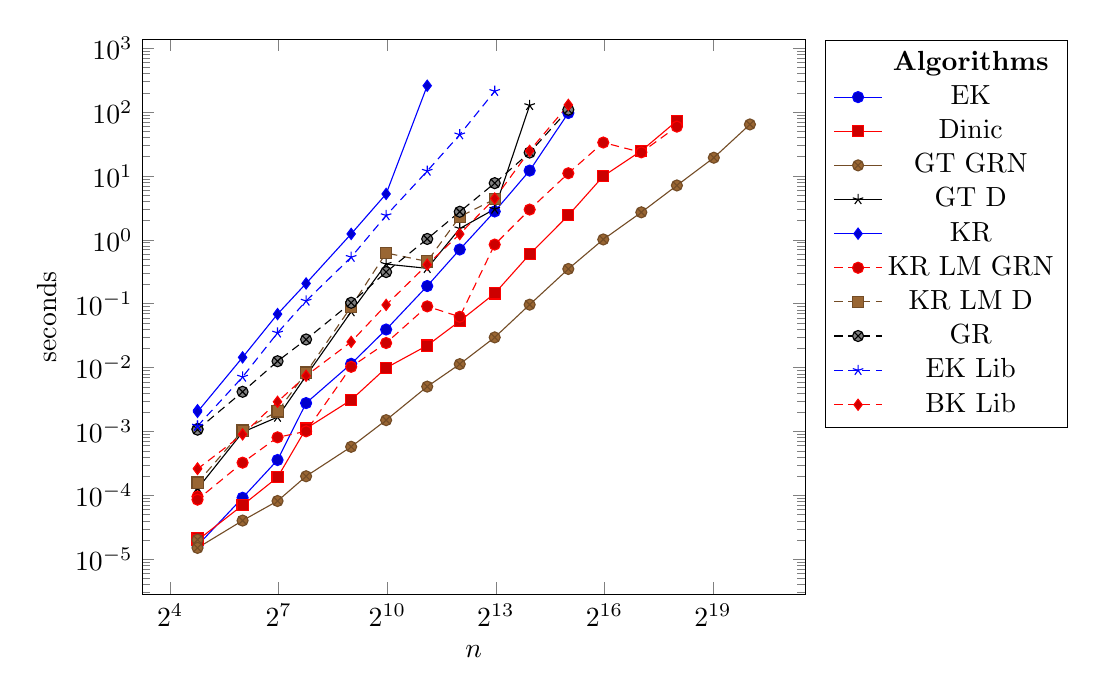
\begin{tikzpicture}
\begin{axis}[
    xlabel=$n$,ylabel=seconds,
    xmode=log,ymode=log,
    log basis x={2},
    legend style=
    {
        legend pos=outer north east
    },
    width=10cm
]
\addlegendimage{legend image code/.code=}
\legend{\textbf{Algorithms}, EK, Dinic, GT GRN, GT D, KR, KR LM GRN, KR LM D, GR, EK Lib, BK Lib}
\addplot table[x=n,y=value] {%EK
n value
27	1.83E-05
27	1.64353E-05
64	9.19488E-05
125	0.000358578
216	0.002789337
512	0.011478267
1000	0.039519567
2197	0.189271
4096	0.706506333
8000	2.78247
15625	12.12773333
32768	96.6569
};
\addplot table[x=n,y=value] {%Dinic
n value
27	2.16546E-05
27	1.98778E-05
64	7.04053E-05
125	0.000192226
216	0.001115157
512	0.003119373
1000	0.00991604
2197	0.0221898
4096	0.053542767
8000	0.144866667
15625	0.59337
32768	2.4171
64000	9.927513333
132651	24.71566667
262144	72.89203333
};
\addplot table[x=n,y=value] {%GT GRN
n value
27	2.03E-05
27	1.51027E-05
64	4.04221E-05
125	8.18436E-05
216	0.000199778
512	0.000577347
1000	0.001509167
2197	0.005050763
4096	0.0113486
8000	0.0297681
15625	0.096823533
32768	0.350279
64000	1.014996667
132651	2.6983
262144	7.101253333
531441	19.29156667
1061208	64.0214
};
\addplot table[x=n,y=value] {%GT D
n value
27	1.33E-04
27	0.000127152
64	0.000977459
125	0.00168207
216	0.007420783
512	0.0751745
1000	0.417246
2197	0.358329333
4096	1.503013333
8000	3.035766667
15625	127.1716667
};
\addplot table[x=n,y=value] {%KR
n value
27	2.16E-03
27	0.002033977
64	0.0144907
125	0.0688899
216	0.207899
512	1.23922
1000	5.23004
2197	258.178
};
\addplot table[x=n,y=value] {%KR LM GRN
n value
27	9.63E-05
27	8.59525E-05
64	0.000325931
125	0.000811551
216	0.001009107
512	0.010306333
1000	0.0242879
2197	0.090985567
4096	0.062492867
8000	0.84353
15625	2.978673333
32768	11.0194
64000	33.353
132651	23.40396667
262144	59.15526667
};
\addplot table[x=n,y=value] {%KR LM D
n value
27	1.61E-04
27	0.000158246
64	0.001037093
125	0.002061527
216	0.008381697
512	0.089949433
1000	0.622961333
2197	0.459367667
4096	2.298873333
8000	4.334706667
};
\addplot table[x=n,y=value] {%GR
n value
27	1.10E-03
27	0.00107007
64	0.004186893
125	0.0125998
216	0.027625867
512	0.103603333
1000	0.313361667
2197	1.03351
4096	2.753226667
8000	7.715346667
15625	23.232
32768	108.9246667
};
\addplot table[x=n,y=value] {%EK Lib
n value
27	0.001224103
27	0.001216997
64	0.007149513
125	0.0350155
216	0.110498333
512	0.535476
1000	2.40563
2197	11.93883333
4096	44.25053333
8000	211.9366667
};
\addplot table[x=n,y=value] {%BK Lib
n value
27	0.000264632
27	0.000259413
64	0.000902392
125	0.002922727
216	0.007462453
512	0.025325933
1000	0.095990433
2197	0.408633667
4096	1.230866667
8000	4.441643333
15625	24.72616667
32768	129.544
};
\end{axis}
\end{tikzpicture}
\caption{Best and worst results from the GenRmf square graphs}
\label{fig:GenRmf square_BW_Results}
\end{figure}

In the following sections we will discuss the performance of each algorithm, but the general performance can be seen from Figure~\ref{fig:GenRmf square_BW_Results}.

\subsection{Choosing $f(G)$ for the GRN Heuristic}
\label{GRNFGSection}

We implemented the GRN heuristic for the algorithms GT GRN, GT D GRN, KR LM GRN and KR LM D GRN. 
The reason we did not implement a KR D GRN algorithm is that previous tests have shown the KR D algorithm to have another bottleneck.
This bottleneck is discussed in Section~\ref{KingRaoResults}.

To find the best function, we tested each algorithm on graphs of the GenRmf and Wash types. 
On each size of graph in each family, we did an exponential search followed by a binary search for the best constant $f(G)=c$ for that particular graph and algorithm.
We did not test on CRE, CD or AK because no flow will have to be pushed back to source in those graphs, so the optimal solution would be to only do one global relabelling at the start of the algorithm.
We also did not test CRH because the construction of this graph is very special, and we believe that the GenRmf and Wash graphs are closer to a typical max flow problem.
Additionally, the GRC heuristic is already optimal for the CRH graphs, because it only does two global relabellings; one at the start, and one right after the minimum cut has been saturated.

We ran each test three times, which yielded about 180 tests per algorithm. We plotted these points, and used a regression tool to find the function on the form $f(G)=an^b$ that best describes the data.
This yielded the following equations

\begin{tabular}{|l|c|c|}
    \hline
    Algorithm & Function & $R^2$ \\\hline\hline
    GT GRN&$f(G)=1.8956n^{0.6548}$&$0.9442$\\\hline
    GT D GRN&$f(G)=0.54n^{0.7144}$&$0.9128$\\\hline
    KR LM GRN&$f(G)=1.5834n^{0.7578}$&$0.7824$\\\hline
    KR LM D GRN&$f(G)=1.6078n^{0.6509}$&$0.6219$\\\hline   
\end{tabular}
\\

Charts of the data points and the regression lines can be seen in Appendix~\ref{GRN_Functions}.




\subsection{Edmonds Karp}

The Edmonds Karp algorithm generally does not perform very well.
Dinic's algorithm is faster than Edmonds Karp, in all examples except for the AK graphs. 
This makes sense with respect to the worstcase time of $O(nm^2)$ for Edmonds Karp, and $O(n^2m)$ for Dinic.
We found that the running time of the Edmonds Karp algorithm is best described as a function of the number of augmenting paths, and the number of edges in the graph.
The more augmenting paths there are, the more breadth first searches will have to be done, and the time for each breath first search depends on the number of edges in the graph.
This is also why its worst case time is $O(nm^2)$. 


\begin{figure}[h]
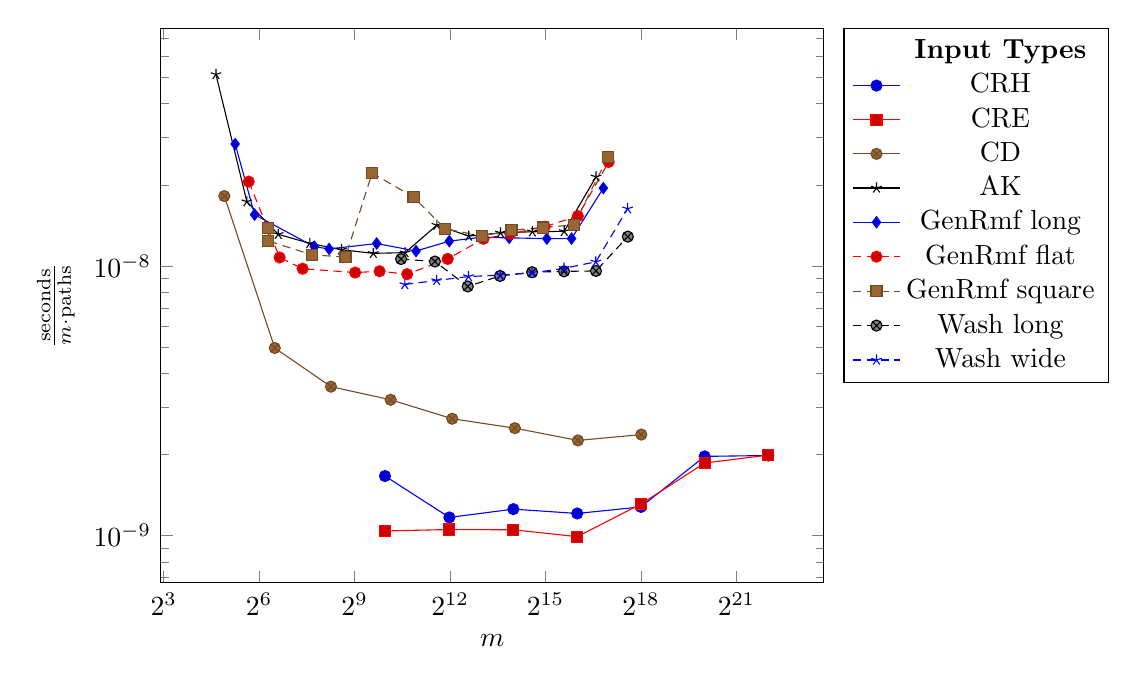
\begin{tikzpicture}
\begin{axis}[
    xlabel=$m$,ylabel=$\frac{\text{seconds}}{m\cdot \text{paths}}$,
    xmode=log,ymode=log,
    log basis x={2},
    legend style=
    {
        legend pos=outer north east
    },
    width=10cm
]
\addlegendimage{legend image code/.code=}
\legend{\textbf{Input Types}, CRH, CRE, CD, AK, GenRmf long, GenRmf flat, GenRmf square, Wash long, Wash wide}
\addplot table[x=n,y=value] {%CRH
n value
992	1.66466E-09
4032	1.16903E-09
16256	1.25451E-09
65280	1.2091E-09
261632	1.27864E-09
1047552	1.96903E-09
4192256	1.98336E-09
};
\addplot table[x=n,y=value] {%CRE
n value
992	1.0413E-09
4032	1.05426E-09
16256	1.05184E-09
65280	9.92107E-10
261632	1.31012E-09
1047552	1.85996E-09
4192256	1.99021E-09
};
\addplot table[x=n,y=value] {%CD
n value
30	1.81717E-08
90	4.96716E-09
306	3.57009E-09
1122	3.19207E-09
4290	2.71479E-09
16770	2.50517E-09
66306	2.25596E-09
263682	2.37129E-09
};
\addplot table[x=n,y=value] {%AK
n value
25	5.13295E-08
49	1.73307E-08
97	1.31136E-08
193	1.21362E-08
385	1.14906E-08
769	1.11464E-08
1537	1.12091E-08
3073	1.41778E-08
6145	1.29195E-08
12289	1.32742E-08
24577	1.34015E-08
49153	1.34511E-08
98305	2.14221E-08
};
\addplot table[x=n,y=value] {%GenRmf long
n value
38	2.83468E-08
58	1.55086E-08
213	1.17957E-08
294	1.15719E-08
828	1.21194E-08
1950	1.13672E-08
4026	1.23664E-08
7868	1.27728E-08
14840	1.27225E-08
33660	1.26353E-08
57717	1.26436E-08
115284	1.94512E-08
};
\addplot table[x=n,y=value] {%GenRmf flat
n value
51	2.05647E-08
100	1.07579E-08
165	9.77235E-09
518	9.45758E-09
882	9.56565E-09
1608	9.32887E-09
3888	1.0626E-08
8484	1.26209E-08
15232	1.31695E-08
32153	1.39854E-08
66150	1.53185E-08
129472	2.43192E-08
};
\addplot table[x=n,y=value] {%GenRmf square
n value
78	1.38184E-08
78	1.23946E-08
204	1.09934E-08
420	1.08071E-08
750	2.21376E-08
1848	1.80034E-08
3690	1.37307E-08
8268	1.29187E-08
15600	1.35717E-08
30780	1.38904E-08
60600	1.42187E-08
127968	2.5442E-08
};
\addplot table[x=n,y=value] {%Wash long
n value
1408	1.06141E-08
2944	1.03926E-08
6016	8.40057E-09
12160	9.18783E-09
24448	9.48726E-09
49024	9.55599E-09
98176	9.58903E-09
196480	1.28548E-08
};
\addplot table[x=n,y=value] {%Wash wide
n value
1528	8.54169E-09
3056	8.84407E-09
6112	9.14132E-09
12224	9.25413E-09
24448	9.42574E-09
48896	9.81213E-09
97792	1.03599E-08
195584	1.63099E-08
};
\end{axis}
\end{tikzpicture}
\caption{Edmonds and Karp performance per $m$ and the number of augmenting paths}
\label{fig:EK_runningTime}
\end{figure}

Figure~\ref{fig:EK_runningTime} shows the time for all measurements of Edmonds Karp, where the running time is divided by the product of the number of edges and the number of augmenting paths in the graph.
Since this chart is mostly flat, $m \cdot \text{\#AugmentingPaths}$ is a good approximation of the running time.
At $m=2^{16}$, the algorithm starts to exit L3 cache, which is the reason for the increase in running time for larger graphs.


\subsection{Dinic}

Dinic's algorithm generally performs well.
It generally beats the push relabel algorithms without heuristics, and many of the heuristics as well. It is not the fastest algorithm in any of our tests though.
It especially has problems on the AK and CD graphs. 
The AK graphs has a low number of augmenting paths in each layer graph. That means that doing a BFS to compute the layer graph, and then a DFS to find the flow in it is slower than just doing a few BFS's to find each augmenting path in the layer graph.
For this reason, we see EK perform better than Dinic on the AK graphs.

Our CRE and CRH graphs are easy for Dinic because there are never more than two layer graphs.
The CD graphs are designed to be hard for Dinic as it has $\Omega(n)$ layer graphs, and as many paths as we could fit in each layer graph. 
We made the CD graph, because we were missing a fully connected graph that Dinic struggles with. 
The results here are better than expected. Dinic does not perform as well as the GT algorithms, but it is not far behind.
The fact that Dinic was so efficient on CD graphs led us to conduct the previous analysis of the number of augmenting paths in the graph.
The observed number of augmenting paths found by Dinic fits well with the $m \log n$ bound achieved by the analysis.
When plotting $\mathrm{Paths}/m\log n$ all points lie on a horizontal line.



\begin{figure}[h]
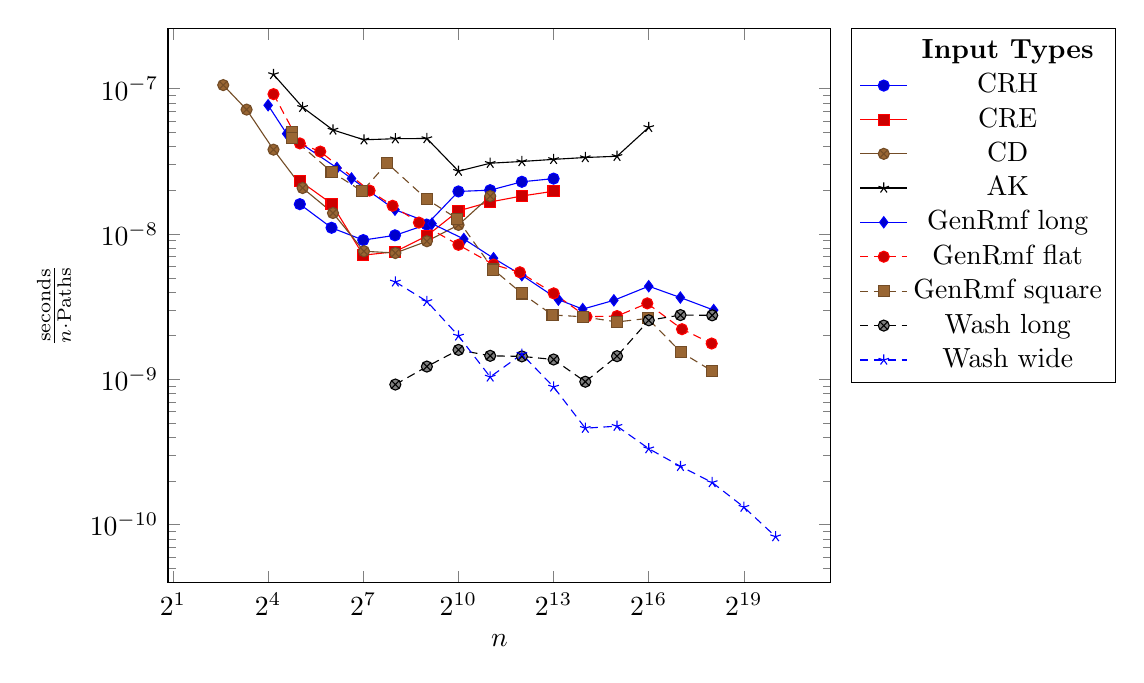
\begin{tikzpicture}
\begin{axis}[
    xlabel=$n$,ylabel=$\frac{\text{seconds}}{n\cdot \text{Paths}}$,
    xmode=log,ymode=log,
    log basis x={2},
    legend style=
    {
        legend pos=outer north east
    },
    width=10cm
]
\addlegendimage{legend image code/.code=}
\legend{\textbf{Input Types}, CRH, CRE, CD, AK, GenRmf long, GenRmf flat, GenRmf square, Wash long, Wash wide}
\addplot table[x=n,y=value] {%CRH
n value
32	1.60662E-08
64	1.10524E-08
128	9.09034E-09
256	9.8052E-09
512	1.16228E-08
1024	1.96589E-08
2048	2.00461E-08
4096	2.29003E-08
8192	2.40805E-08
};
\addplot table[x=n,y=value] {%CRE
n value
32	2.32243E-08
64	1.61998E-08
128	7.16023E-09
256	7.55879E-09
512	9.70943E-09
1024	1.44429E-08
2048	1.66357E-08
4096	1.82794E-08
8192	1.97247E-08
};
\addplot table[x=n,y=value] {%CD
n value
6	1.06002E-07
10	7.18898E-08
18	3.81028E-08
34	2.07454E-08
66	1.39579E-08
130	7.62282E-09
258	7.40559E-09
514	8.92618E-09
1026	1.1564E-08
2050	1.82553E-08
};
\addplot table[x=n,y=value] {%AK
n value
18	1.25445E-07
34	7.45452E-08
66	5.20575E-08
130	4.45512E-08
258	4.5328E-08
514	4.54889E-08
1026	2.71015E-08
2050	3.07429E-08
4098	3.15994E-08
8194	3.2674E-08
16386	3.36491E-08
32770	3.43191E-08
65538	5.42947E-08
};
\addplot table[x=n,y=value] {%GenRmf long
n value
16	7.70404E-08
24	4.90468E-08
72	2.85335E-08
99	2.41266E-08
256	1.47136E-08
575	1.17925E-08
1152	9.25426E-09
2205	6.82108E-09
4096	5.21221E-09
9100	3.54137E-09
15488	3.04506E-09
30589	3.50078E-09
65536	4.37844E-09
130682	3.65803E-09
270848	2.99932E-09
};
\addplot table[x=n,y=value] {%GenRmf flat
n value
18	9.18556E-08
32	4.20773E-08
50	3.69572E-08
147	1.99257E-08
243	1.5665E-08
432	1.19976E-08
1024	8.43176E-09
2205	6.16549E-09
3920	5.46192E-09
8214	3.90928E-09
16807	2.70144E-09
32768	2.72785E-09
63504	3.33529E-09
135531	2.21539E-09
259308	1.76556E-09
};
\addplot table[x=n,y=value] {%GenRmf square
n value
27	5.01265E-08
27	4.60135E-08
64	2.68313E-08
125	1.97155E-08
216	3.07307E-08
512	1.74072E-08
1000	1.27292E-08
2197	5.6998E-09
4096	3.90324E-09
8000	2.77607E-09
15625	2.69714E-09
32768	2.48514E-09
64000	2.62866E-09
132651	1.5397E-09
262144	1.14193E-09
};
\addplot table[x=n,y=value] {%Wash long
n value
258	9.21744E-10
514	1.22555E-09
1026	1.59596E-09
2050	1.45298E-09
4098	1.44002E-09
8194	1.37073E-09
16386	9.63818E-10
32770	1.4445E-09
65538	2.55088E-09
131074	2.77054E-09
262146	2.75927E-09
};
\addplot table[x=n,y=value] {%Wash wide
n value
258	4.6875E-09
514	3.44298E-09
1026	1.9923E-09
2050	1.03997E-09
4098	1.49151E-09
8194	8.8731E-10
16386	4.61535E-10
32770	4.76501E-10
65538	3.33716E-10
131074	2.52127E-10
262146	1.95298E-10
524290	1.32129E-10
1048578	8.27744E-11
};
\end{axis}
\end{tikzpicture}
\caption{Dinic performance per $nP$}
\label{fig:Dinic_runningTime}
\end{figure}

With regard to the running time, we found that the running time of Dinic was mostly proportional to $n$ times the total number of paths the algorithm found.
This can be seen on Figure~\ref{fig:Dinic_runningTime}.
Here we divided the running time in each test by $n\cdot \text{Paths}$.
Many of the graphs, such as the GenRmf and Wash graphs, seems to be faster than $n\cdot\text{Paths}$. 
We believe the problem is that not all paths are of length $n$. For many of the layer graphs, $k$ is a lot smaller than $n$.
In fact, as $k$ approach $n$, the layer graph will not be able to contain as many paths as when $k$ is significantly smaller than $n$.
For example, if $k=n$, there can only be one augmenting path that contains all nodes.
This means that $n$ is an over estimation on the average length of the augmenting paths.

\subsection{Goldberg Tarjan}

The Goldberg Tarjan algorithms perform very well, especially with the heuristics.
Before the heuristics, GT was the fastest on the CRE, CD and AK graphs. 
With heuristics, in all our tests, it is always some version of GT that is the fastest.

It makes good sense that GT is the fastest on the CRE, CD and AK graphs. CRE is basically the best case graph for GT, because it can ignore the majority of all the edges due to the fact that nodes never go above a label of 2.
The reason the maximum label is two is that a node is only relabelled from $1$ to $2$ when no more flow can be sent to the target node.
The graph is fully connected with very high capacities, so once a node has been relabelled to $2$, it will be able to send all its excess to a node with label $1$.

The GRH graphs on the other hand is the worst case for this algorithm.
All nodes will have to be relabelled to $n$ before the algorithm can terminate. In-between the relabels, the algorithm will also spend time pushing the excess back and forth between nodes.
That is why, without heuristics, the GT algorithm falls far behind Dinic on the CRH graphs.

The Goldberg Tarjan algorithm has an advantage in the CD graphs, because no flow will ever have to be pushed back to source. 
The way the CD graphs are constructed, no edge has more capacity than what is needed to get the flow to the target node.
The maximum label depends on the order the algorithm processes the nodes. For each CD graph, there is one order which results in no nodes getting a label higher than $2$.
There is also an order that results in nodes having labels $n$, $n-1$, $n-2$, etc. Regardless of the label, the same number of pushes is required though.



\begin{figure}[h]
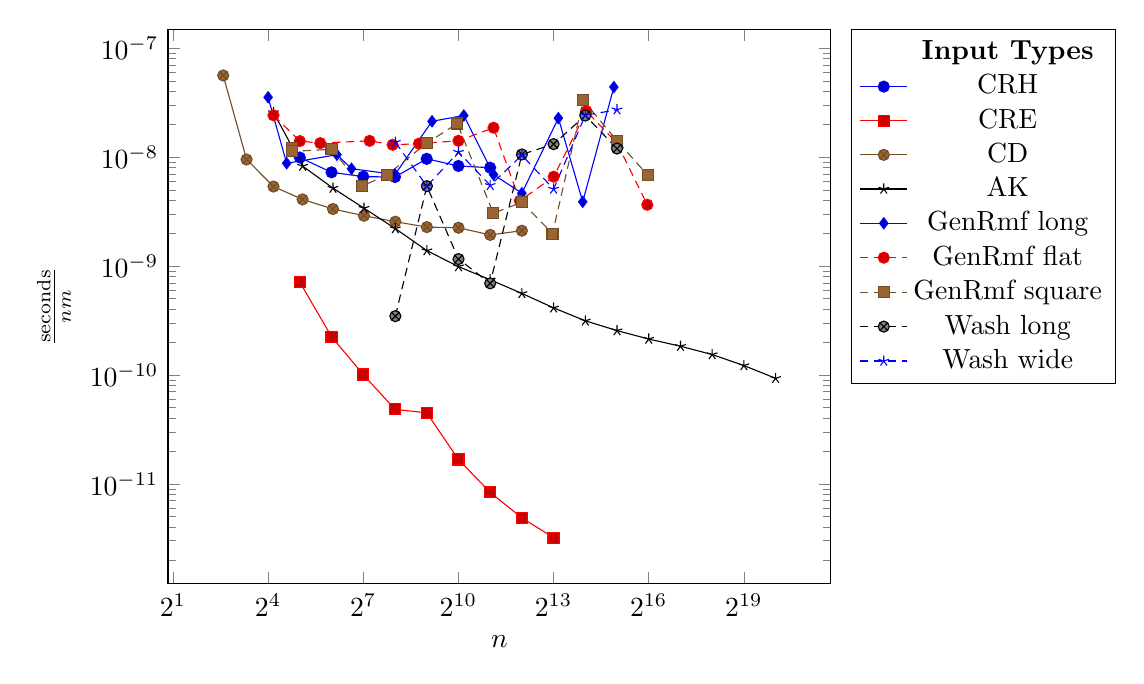
\begin{tikzpicture}
\begin{axis}[
    xlabel=$n$,ylabel=$\frac{\text{seconds}}{nm}$,
    xmode=log,ymode=log,
    log basis x={2},
    legend style=
    {
        legend pos=outer north east
    },
    width=10cm
]
\addlegendimage{legend image code/.code=}
\legend{\textbf{Input Types}, CRH, CRE, CD, AK, GenRmf long, GenRmf flat, GenRmf square, Wash long, Wash wide}
\addplot table[x=n,y=value] {%CRH
n value
32	9.90712E-09
64	7.24742E-09
128	6.61376E-09
256	6.56429E-09
512	9.63395E-09
1024	8.2859E-09
2048	7.99078E-09
};
\addplot table[x=n,y=value] {%CRE
n value
32	7.1015E-10
64	2.24209E-10
128	1.00655E-10
256	4.82229E-11
512	4.48739E-11
1024	1.67318E-11
2048	8.34562E-12
4096	4.86383E-12
8192	3.20329E-12
};
\addplot table[x=n,y=value] {%CD
n value
6	5.61416E-08
10	9.50089E-09
18	5.36295E-09
34	4.08415E-09
66	3.33572E-09
130	2.89291E-09
258	2.55076E-09
514	2.27462E-09
1026	2.24389E-09
2050	1.92973E-09
4098	2.10844E-09
};
\addplot table[x=n,y=value] {%AK
n value
18	2.56647E-08
34	8.26537E-09
66	5.18647E-09
130	3.39477E-09
258	2.20466E-09
514	1.38395E-09
1026	9.86652E-10
2050	7.47385E-10
4098	5.60005E-10
8194	4.12565E-10
16386	3.13874E-10
32770	2.54984E-10
65538	2.13448E-10
131074	1.83323E-10
262146	1.53786E-10
524290	1.21857E-10
1048578	9.30332E-11
};
\addplot table[x=n,y=value] {%GenRmf long
n value
16	3.54335E-08
24	8.77545E-09
72	1.05068E-08
99	7.81762E-09
256	6.92696E-09
575	2.13165E-08
1152	2.40867E-08
2205	6.90549E-09
4096	4.66368E-09
9100	2.27639E-08
15488	3.88656E-09
30589	4.39229E-08
};
\addplot table[x=n,y=value] {%GenRmf flat
n value
18	2.41938E-08
32	1.402E-08
50	1.34336E-08
147	1.40864E-08
243	1.29601E-08
432	1.32838E-08
1024	1.41106E-08
2205	1.8587E-08
3920	3.968E-09
8214	6.60992E-09
16807	2.63829E-08
32768	1.34006E-08
63504	3.647E-09
};
\addplot table[x=n,y=value] {%GenRmf square
n value
27	1.20752E-08
27	1.12842E-08
64	1.17888E-08
125	5.41498E-09
216	6.87753E-09
512	1.34166E-08
1000	2.0345E-08
2197	3.04784E-09
4096	3.8493E-09
8000	1.98347E-09
15625	3.31797E-08
32768	1.41112E-08
64000	6.83458E-09
};
\addplot table[x=n,y=value] {%Wash long
n value
258	3.46356E-10
514	5.40945E-09
1026	1.15649E-09
2050	6.92953E-10
4098	1.05799E-08
8194	1.31438E-08
16386	2.40597E-08
32770	1.19685E-08
};
\addplot table[x=n,y=value] {%Wash wide
n value
258	1.36924E-08
514	5.40668E-09
1026	1.11032E-08
2050	5.50623E-09
4098	1.03918E-08
8194	5.09109E-09
16386	2.41668E-08
32770	2.72197E-08
};
\end{axis}
\end{tikzpicture}
\caption{GT performance per $nm$}
\label{fig:GT_runningTime}
\end{figure}

\begin{figure}[h]
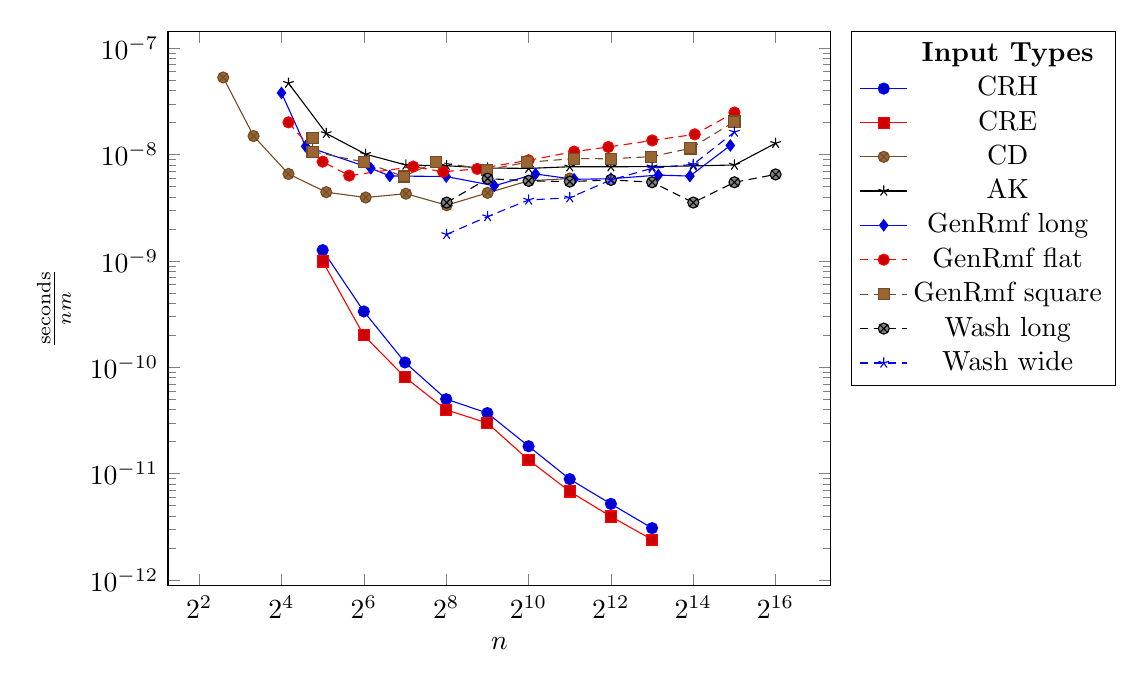
\begin{tikzpicture}
\begin{axis}[
    xlabel=$n$,ylabel=$\frac{\text{seconds}}{nm}$,
    xmode=log,ymode=log,
    log basis x={2},
    legend style=
    {
        legend pos=outer north east
    },
    width=10cm
]
\addlegendimage{legend image code/.code=}
\legend{\textbf{Input Types}, CRH, CRE, CD, AK, GenRmf long, GenRmf flat, GenRmf square, Wash long, Wash wide}
\addplot table[x=n,y=value] {%CRH
n value
32	1.26288E-09
64	3.35238E-10
128	1.11168E-10
256	5.03027E-11
512	3.71824E-11
1024	1.81421E-11
2048	8.90429E-12
4096	5.20555E-12
8192	3.0819E-12
};
\addplot table[x=n,y=value] {%CRE
n value
32	9.90013E-10
64	1.9968E-10
128	8.07477E-11
256	3.98834E-11
512	2.99502E-11
1024	1.35027E-11
2048	6.81994E-12
4096	3.96241E-12
8192	2.40243E-12
};
\addplot table[x=n,y=value] {%CD
n value
6	5.30569E-08
10	1.49299E-08
18	6.57264E-09
34	4.43056E-09
66	3.94952E-09
130	4.2887E-09
258	3.3403E-09
514	4.36561E-09
1026	5.66833E-09
2050	5.95279E-09
};
\addplot table[x=n,y=value] {%AK
n value
18	4.68876E-08
34	1.57975E-08
66	1.0078E-08
130	7.98015E-09
258	7.84601E-09
514	7.4766E-09
1026	7.41183E-09
2050	7.68286E-09
4098	7.68821E-09
8194	7.69572E-09
16386	7.82987E-09
32770	7.98256E-09
65538	1.27783E-08
};
\addplot table[x=n,y=value] {%GenRmf long
n value
16	3.79906E-08
24	1.19665E-08
72	7.4366E-09
99	6.29532E-09
256	6.21655E-09
575	5.09247E-09
1152	6.56912E-09
2205	5.85557E-09
4096	5.92566E-09
9100	6.41111E-09
15488	6.27912E-09
30589	1.21796E-08
};
\addplot table[x=n,y=value] {%GenRmf flat
n value
18	2.00808E-08
32	8.57161E-09
50	6.33991E-09
147	7.7075E-09
243	6.89168E-09
432	7.32937E-09
1024	8.83296E-09
2205	1.06628E-08
3920	1.1773E-08
8214	1.3578E-08
16807	1.54848E-08
32768	2.48237E-08
};
\addplot table[x=n,y=value] {%GenRmf square
n value
27	1.43953E-08
27	1.06515E-08
64	8.51412E-09
125	6.22088E-09
216	8.53572E-09
512	7.21217E-09
1000	8.45903E-09
2197	9.16498E-09
4096	9.1337E-09
8000	9.54867E-09
15625	1.14186E-08
32768	2.04167E-08
};
\addplot table[x=n,y=value] {%Wash long
n value
258	3.53846E-09
514	5.93937E-09
1026	5.66374E-09
2050	5.56832E-09
4098	5.78294E-09
8194	5.49482E-09
16386	3.53918E-09
32770	5.49036E-09
65538	6.50731E-09
};
\addplot table[x=n,y=value] {%Wash wide
n value
258	1.77663E-09
514	2.61444E-09
1026	3.74229E-09
2050	3.93122E-09
4098	5.77718E-09
8194	7.43357E-09
16386	8.0869E-09
32770	1.62903E-08
};
\end{axis}
\end{tikzpicture}
\caption{GT GRC performance per $nm$}
\label{fig:GT_GRC_runningTime}
\end{figure}

The algorithm will have to push flow back to the source in the AK graph, but this is only for the two nodes right next to the source.
All other nodes is able to push all their excess to the target node, so the algorithm won't have to spend time relabelling a lot of nodes to get flow back to the source.
There are long paths in the graph though, so labels get high even though all the excess is pushed to the target.


It seems apparent that the running time of the GT algorithm is directly proportional to the number of relabels required.
When we try to compare it to $O(n^3)$ or $O(nm)$, we get a lot of big jumps up and down in the results.
This tells us that there is something other than $n$ and $m$ that has a big impact on the running time.
As can be seen from Figure~\ref{fig:GT_runningTime}, the jumps comes from the GenRmf and Washington graphs. 
We found that the jumps are caused by the randomized capacities in the GenRmf and Washington.
If we consider the minimum cut in such a graph, which is an $(S, T)$ cut, then the problem is that the size of the set $S$ can get very big.
All nodes in $S$ would have to be relabelled above $n$ in order for the excess to be sent back to $s$.
This means that if the size of $S$ is big in one graph and small in another, even though the second graph is bigger than the first, 
the second graph could be solved faster.


This is the reason we decided to implement the global relabelling heuristics. 
As can be seen from Figure~\ref{fig:GT_GRC_runningTime}, the jumps disappeared when we implemented the GRC heuristic.
This is because the algorithm no longer has to relabel the nodes in $S$ all the way to $n$ one step at the time.

Based on the data in Figure~\ref{fig:GT_runningTime}, it seems that the GT algorithm is a faster than $nm$ for the AK and CRE graphs.
CD and CRH graphs seems to be levelling out towards the end of their chart, but we do not have enough points to be sure. 
It would seem that $nm$ is a better estimate for the running time of GT than the worst case bound of $O(n^3)$ in our test data.

The GT D algorithm has the same jumps as the GT algorithm. 
The effect of dynamic trees are described in Section~\ref{Dynamic Trees Section}.
Additionally, the benefits and drawbacks of the different heuristics are described in Section~\ref{Global Relabelling Section}.

\subsection{King Rao}
\label{KingRaoResults}

The KR D, KR D GRC, KR D GRP algorithms are the worst algorithms in every test we have done.
The problem is that the game requires $2n^2$ nodes and $nm$ edges.
This results in the issue that every time a node is relabelled, a new node in the game will have to be loaded from main memory, or possibly even the hard disk.
We do however not have any examples where the algorithm went to the disk, because it failed with a memory allocation error for large inputs.
The performance is only worse when going to the disk, so running for larger inputs will not yield any new information. For this reason, we did not want to investigate this error further.
We did not see any major improvements when using the GRC or GRP heuristics on this algorithm.
As mentioned in Section~\ref{HeuristicsSection}, the problem is that we can not efficiently relabel a node multiple steps at a time since the data structure has to be updated for all the labels in-between.
These three algorithms perform about the same in all of our tests. An example can be seen in Figure~\ref{fig:GenRmf long_KR_Results}.
Since there is no benefit from the other heuristics, we decided not to spend time on implementing the GRN heuristic for the KR D algorithm.



\begin{figure}[h]
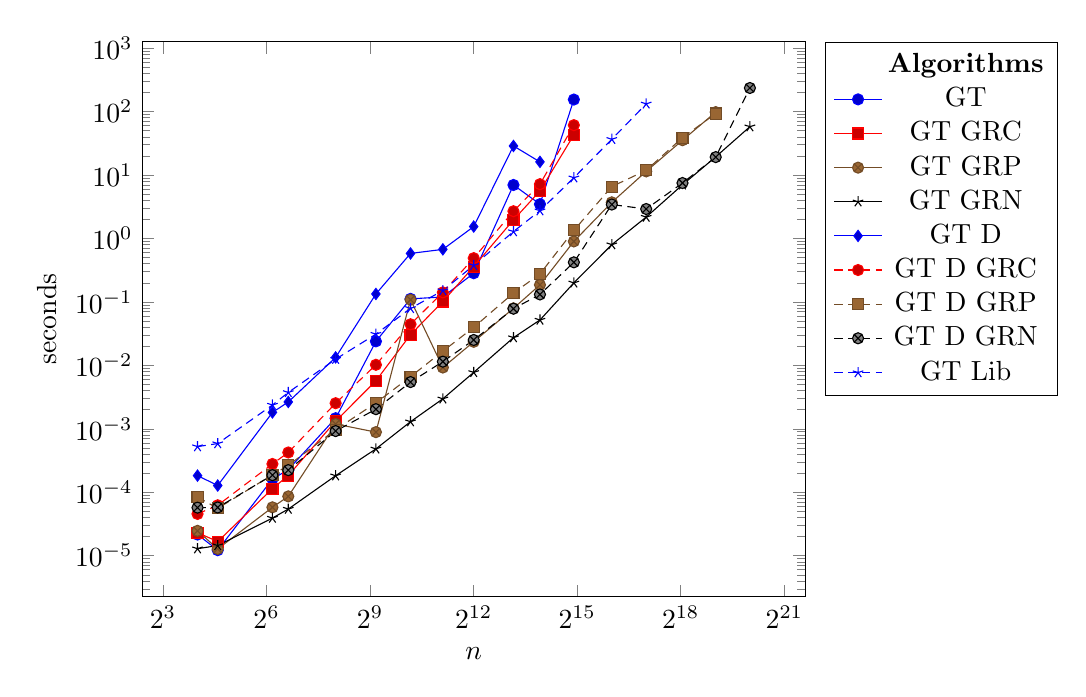
\begin{tikzpicture}
\begin{axis}[
    xlabel=$n$,ylabel=seconds,
    xmode=log,ymode=log,
    log basis x={2},
    legend style=
    {
        legend pos=outer north east
    },
    width=10cm
]
\addlegendimage{legend image code/.code=}
\legend{\textbf{Algorithms}, GT, GT GRC, GT GRP, GT GRN, GT D, GT D GRC, GT D GRP, GT D GRN, GT Lib}
\addplot table[x=n,y=value] {%GT
n value
16	2.15436E-05
24	1.22154E-05
72	0.000161133
99	0.00022754
256	0.001468293
575	0.023901133
1152	0.111713
2205	0.119803
4096	0.28348
9100	6.972716667
15488	3.47428
30589	154.8906667
};
\addplot table[x=n,y=value] {%GT GRC
n value
16	2.30983E-05
24	1.66574E-05
72	0.000114048
99	0.000183232
256	0.00131771
575	0.005709937
1152	0.030467267
2205	0.101588
4096	0.360189
9100	1.96376
15488	5.613036667
30589	42.95033333
};
\addplot table[x=n,y=value] {%GT GRP
n value
16	2.4653E-05
24	1.27707E-05
72	5.78567E-05
99	8.60632E-05
256	0.001188007
575	0.000886396
1152	0.108298
2205	0.009246077
4096	0.0235188
9100	0.079296967
15488	0.185714333
30589	0.899061333
65536	3.712403333
130682	11.41563333
270848	35.41273333
527796	98.1075
};
\addplot table[x=n,y=value] {%GT GRN
n value
16	1.28818E-05
24	1.44365E-05
72	3.92005E-05
99	5.43033E-05
256	0.000182232
575	0.000482289
1152	0.001294393
2205	0.002970023
4096	0.00775149
9100	0.0273884
15488	0.051847533
30589	0.199656667
65536	0.799864667
130682	2.173773333
270848	7.017736667
527796	19.36696667
1048576	57.80963333
};
\addplot table[x=n,y=value] {%GT D
n value
16	0.000182899
24	0.000127707
72	0.001811667
99	0.002649647
256	0.01333294
575	0.133493
1152	0.581190667
2205	0.673778667
4096	1.540246667
9100	28.75023333
15488	16.11123333
};
\addplot table[x=n,y=value] {%GT D GRC
n value
16	4.55303E-05
24	6.22988E-05
72	0.000279179
99	0.000423655
256	0.00253193
575	0.010205033
1152	0.044468633
2205	0.141443667
4096	0.490048
9100	2.690203333
15488	7.183683333
30589	61.1455
};
\addplot table[x=n,y=value] {%GT D GRP
n value
16	8.40646E-05
24	5.57469E-05
72	0.000188007
99	0.000264631
256	0.000967909
575	0.002560693
1152	0.006632443
2205	0.016727867
4096	0.039698667
9100	0.138222667
15488	0.27566
30589	1.342566667
65536	6.573553333
130682	11.86123333
270848	38.87526667
527796	93.12866667
};
\addplot table[x=n,y=value] {%GT D GRN
n value
16	5.71906E-05
24	5.75237E-05
72	0.000186008
99	0.000223099
256	0.000920491
575	0.002039097
1152	0.005452093
2205	0.011442267
4096	0.025133533
9100	0.078167533
15488	0.131162333
30589	0.420732667
65536	3.42981
130682	2.91399
270848	7.486506667
527796	19.16753333
1048576	235.5196667
};
\addplot table[x=n,y=value] {%GT Lib
n value
16	0.000524045
24	0.000584789
72	0.002370587
99	0.003742273
256	0.012512867
575	0.031066333
1152	0.079139833
2205	0.151054
4096	0.376943
9100	1.286306667
15488	2.73918
30589	9.066496667
65536	36.64306667
130682	132.3713333
};
\end{axis}
\end{tikzpicture}
\caption{Goldberg and Tarjan results from the GenRmf long graphs}
\label{fig:GenRmf long_GT_Results}
\end{figure}


\begin{figure}[h]
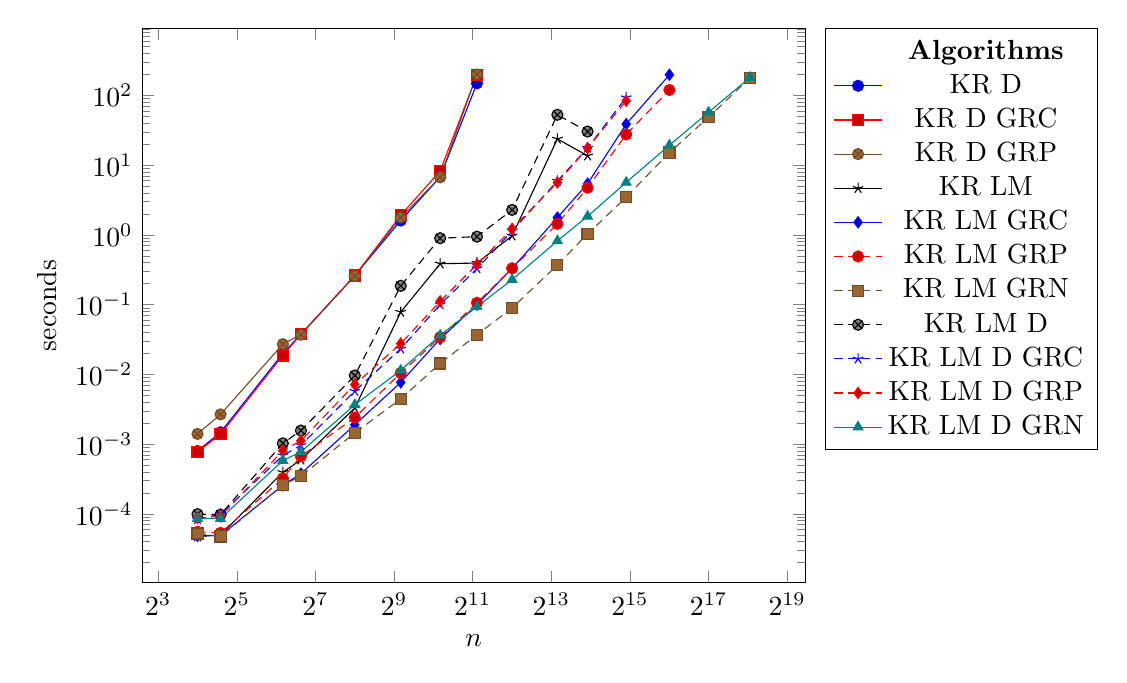
\begin{tikzpicture}
\begin{axis}[
    xlabel=$n$,ylabel=seconds,
    xmode=log,ymode=log,
    log basis x={2},
    legend style=
    {
        legend pos=outer north east
    },
    width=10cm
]
\addlegendimage{legend image code/.code=}
\legend{\textbf{Algorithms}, KR D, KR D GRC, KR D GRP, KR LM, KR LM GRC, KR LM GRP, KR LM GRN, KR LM D, KR LM D GRC, KR LM D GRP, KR LM D GRN}
\addplot table[x=n,y=value] {%KR
n value
16	0.000795004
24	0.00147618
72	0.019901867
99	0.037501367
256	0.260456667
575	1.606663333
1152	6.740186667
2205	149.337
};
\addplot table[x=n,y=value] {%KR GRC
n value
16	0.000769905
24	0.001389337
72	0.018663067
99	0.0377529
256	0.261381
575	1.908376667
1152	8.252073333
2205	197.4756667
};
\addplot table[x=n,y=value] {%KR GRP
n value
16	0.00139845
24	0.002666637
72	0.0271098
99	0.037121367
256	0.258182333
575	1.773686667
1152	6.72207
2205	200.141
};
\addplot table[x=n,y=value] {%KR LM
n value
16	4.70851E-05
24	4.97503E-05
72	0.000394004
99	0.000594782
256	0.003290843
575	0.078265033
1152	0.385737667
2205	0.395114667
4096	0.969813
9100	23.78033333
15488	13.6657
};
\addplot table[x=n,y=value] {%KR LM GRC
n value
16	4.81955E-05
24	4.90839E-05
72	0.000255858
99	0.000376681
256	0.001889957
575	0.007676197
1152	0.0321853
2205	0.099800333
4096	0.331238
9100	1.773373333
15488	5.421613333
30589	38.8194
65536	197.752
};
\addplot table[x=n,y=value] {%KR LM GRP
n value
16	5.53027E-05
24	5.31928E-05
72	0.000322266
99	0.000671628
256	0.002406003
575	0.010445347
1152	0.034050267
2205	0.10638
4096	0.331282667
9100	1.439603333
15488	4.751253333
30589	27.6015
65536	119.7773333
};
\addplot table[x=n,y=value] {%KR LM GRN
n value
16	5.21933E-05
24	4.73072E-05
72	0.000259523
99	0.000345365
256	0.001449643
575	0.00443921
1152	0.014312
2205	0.037018833
4096	0.089594333
9100	0.369817
15488	1.033306667
30589	3.473556667
65536	15.1593
130682	48.64013333
270848	178.9876667
};
\addplot table[x=n,y=value] {%KR LM D
n value
16	9.88343E-05
24	9.73907E-05
72	0.001024097
99	0.001562027
256	0.009612567
575	0.186065333
1152	0.896549
2205	0.943830667
4096	2.28156
9100	52.7981
15488	30.36093333
};
\addplot table[x=n,y=value] {%KR LM D GRC
n value
16	8.31763E-05
24	9.87233E-05
72	0.000685843
99	0.000960468
256	0.00575304
575	0.023246133
1152	0.100415667
2205	0.328566333
4096	1.139136667
9100	5.931156667
15488	17.6933
30589	93.37536667
};
\addplot table[x=n,y=value] {%KR LM D GRP
n value
16	8.69519E-05
24	9.19491E-05
72	0.000803777
99	0.001117273
256	0.007166817
575	0.027587633
1152	0.111327333
2205	0.376117333
4096	1.221456667
9100	5.651543333
15488	17.5763
30589	83.79273333
};
\addplot[mark=triangle*, teal] table[x=n,y=value] {%KR LM D GRN
n value
16	8.53971E-05
24	8.53972E-05
72	0.000580235
99	0.000774794
256	0.00366275
575	0.011421333
1152	0.036280633
2205	0.0934643
4096	0.228176333
9100	0.820808667
15488	1.847203333
30589	5.658126667
65536	19.2994
130682	57.2744
270848	180.989
};
\end{axis}
\end{tikzpicture}
\caption{King and Rao results from the GenRmf long graphs}
\label{fig:GenRmf long_KR_Results}
\end{figure}


The LM versions behave similar to the corresponding GT algorithms, except that they are slower.
A good example of this can be seen from comparing Figure~\ref{fig:GenRmf long_GT_Results} with Figure~\ref{fig:GenRmf long_KR_Results}. 
If you look at KR LM and KR LM D in Figure~\ref{fig:GenRmf long_KR_Results} and compare the curves to GT and GT D in Figure~\ref{fig:GenRmf long_GT_Results}, you see that the curves have the same ups and downs, but the KR algorihms are slower.
The main difference between the GT algorithms and the KR LM algorithms is the choice of current edges.
In our tests, the overhead that results from the more complicated way of choosing current edges is far greater than any time saved.
We have no example where the fastest KR algorithm beats the fastest GT algorithm, but KR LM D does beat GT D on GenRmf and Wash graphs.

When we first ran our different implementations of the King Rao algorithm, we observed big differences in running time between runs on the same graph, especially on the AK graphs.
As an example, when we tested KR LM D GRP on an AK graph with $n=8194$, we got results in the range from $0.21$ seconds to $6.61$ seconds.
This was unexpected, since the algorithm is not randomized, and it is the exact same input. 
We managed to track the issue down to the initial sorting of the edges according to unsigned capacity. 
We used the implementation of quick sort from the c++ library, which is not a stable sort. If two edges have the same unsigned capacity, the position of them relative to each other is random.
We managed to get consistent results by making sure that the comparator we use never returns $0$. With this, we got the example above down to $0,06$ seconds.
This shows that the order in which the edges are added has a very big impact on the running time. 
It affects in the order in which nodes a processed, because the act of adding an edge modifies the amount of visible edges on the nodes next to the edge.
In the AK graphs, many edges have the same capacity, so the the issue can have a very big effect on graphs of this type.
The results displayed for the KR algorithms in the charts are results from after we made the sorting deterministic.

\subsection{Goldberg Rao}

The GR algorithm is slower than most of our other algorithms.
The only algorithms that are consistently worse than GR are the KR algorithms without memory optimizations.
On some graphs, GR does beat the KR LM and GT algorithms without heuristics on large inputs.
We think that the reasons that GR is so slow compared to the other algorithm is mainly that it is doing a lot of different things, 
which means it has allocated a lot more memory than the others. 
All the memory is being used at some point in the main loop of the algorithm, so it will have to swap memory between caches more often than the other algorithms.
Also, we have not spent much time on locating and removing bottlenecks in this algorithm or on tweaking the constants.

Tweaking the constants is something we think could make a big difference.
We see big differences in the running time of GR on long and wide GenRmf graphs.
On GenRmf graphs, the edges within each layer has capacities $10000a^2$, which is needed to route all flow that could be sent between layers.
The first cut of the graph used to bound $F$ in the algorithm is going to be made between $s$ and the rest of the graph.
This cut contains two edges with $10000a^2$ capacity and one edge with a random capacity up to 10000.
So after the first iteration, $F=20000a^2$, which influences $\Delta$.
On long GenRmf graphs, $b=a^2$, which means that $a$ is and by extension the capacities on the edges inside the layers are small compared to capacities on edges between layers.
This causes $F$ and by extension $\Delta$ to be very small after the first iteration. 
The differences in capacity on edges inside layers and edges between layers is so small that after saturating an edge between each layer, all nodes become a single connected component.
That means that in the majority of the iterations, the algorithm does not run the blocking flow algorithm, but just routes $\Delta$ flow inside the big connected component.

On the wide GenRmf graphs however, edges inside the layers have a very big capacity compared to the edges between the layers.
This causes $F$ and by extension $\Delta$ to be so big that only edges inside layers are going to be zero length arcs.
The first layer graph where connected components are formed will be single list of super nodes.

In both cases, we can send about $5000a^2$ on average between the cuts. 
We are only allowed to send $\Delta = F/\Lambda = 20000a^2/\Lambda$ units of flow from $s$ to $t$.
Since GenRmf graphs are very sparse, we get $\Lambda=\sqrt{m}=O(\sqrt{n})$.
So when $n>16$, $\Delta$ becomes so small that we are not allowed to send $5000a^2$ units of flow, which means we wont be able to send the max flow in the first iterations.

If we experimented with other values of $\Delta$, we could get the wide GenRmf graphs to solve the max flow problem in very few steps.
In the wide GenRmf graphs, the layer graph will consist of a single path of super nodes, and the minimum cut will be between two of them.
If $\Delta$ allowed this cut to be saturated, the algorithm would be finished.
 
We see a similar story in the wash graphs. In the long version, the cuts contain few edges which results in a low $\Delta$ compared to the capacity on the edges 
as opposed to the wide version where there is a lot of edges in the cuts.
Also here, the long version with the relatively low $\Delta$ is faster.
After flow has been sent on a path $(s, v_1, \ldots, v_k, t)$ in the long version, a connected component can form from the smallest 
$i$ and largest $j$ such that there is an alternate path from $v_i$ to $v_j$.
Any other alternate paths from $v_k$ to $v_l$ where $i\leq k < l \leq j$ would also be part of that connected component.
As soon as two connected components share a node, they become one connected component.
This results in very quickly getting the entire graph into one connected component.

What takes time depends heavily on how $\Delta$ is in relation to the capacities on the edges, which affects how strongly connected components are formed.
In graphs that almost only consist of strongly connected components, we naturally see almost no time spent on the blocking flow algorithm.
Vice versa, if the graph has few strongly connected components, a lot of the time is spent on the blocking flow algorithm.
If we compare GenRmf long, wide and square graphs of the same size, then GR is fastest on the long graphs and slowest on the wide graphs with the square ones in between.
We would like to have some input graphs where we can vary the number and size of connected components without changing the result of the algorithm or the resulting flow graph.
That would give us a more clear image of the trade off between spending time on connected components and spending time on the blocking flow algorithm.
Based on the results we have now, it would seem that bigger is better in terms of strongly connected components.


\subsection{Dynamic Trees}
\label{Dynamic Trees Section}
Dynamic trees tend to make the running time op the algorithms slightly worse. It does not change the running time as much as heuristics can, but it does make it slower.
A good example is Figure~\ref{fig:GenRmf square_GT_Results}, where we see every dynamic version of GT being slightly slower than its non dynamic counterpart.


\begin{figure}[h]
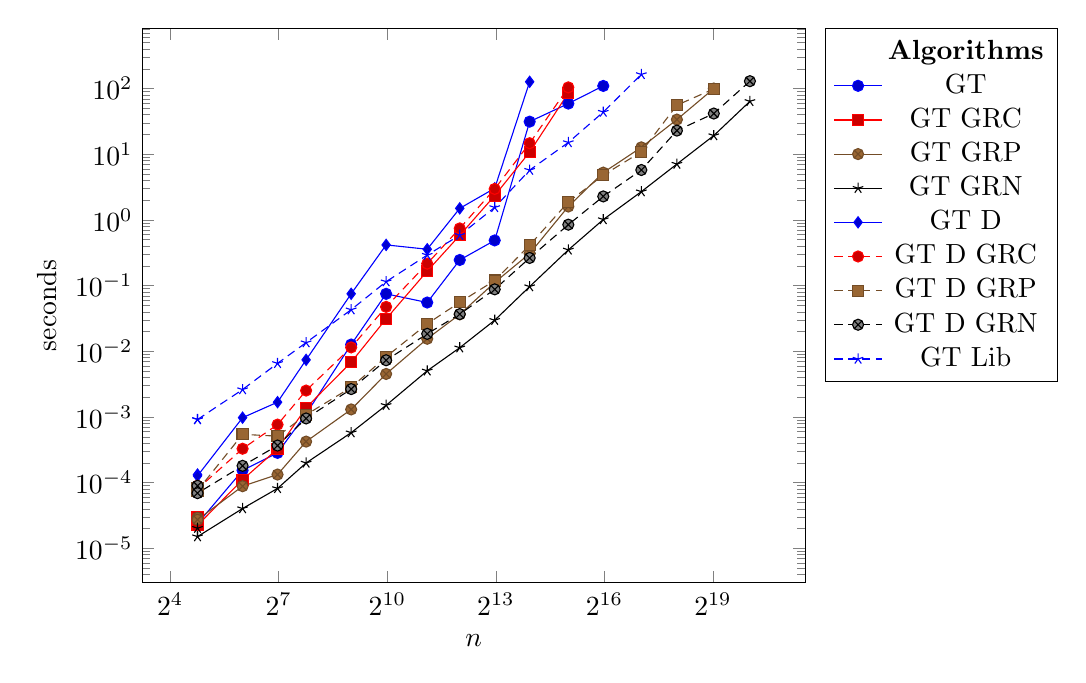
\begin{tikzpicture}
\begin{axis}[
    xlabel=$n$,ylabel=seconds,
    xmode=log,ymode=log,
    log basis x={2},
    legend style=
    {
        legend pos=outer north east
    },
    width=10cm
]
\addlegendimage{legend image code/.code=}
\legend{\textbf{Algorithms}, GT, GT GRC, GT GRP, GT GRN, GT D, GT D GRC, GT D GRP, GT D GRN, GT Lib}
\addplot table[x=n,y=value] {%GT
n value
27	2.54E-05
27	2.37646E-05
64	0.000153914
125	0.000284286
216	0.00111416
512	0.0126945
1000	0.075073033
2197	0.055363333
4096	0.245961333
8000	0.488409
15625	31.41703333
32768	59.17186667
64000	109.8606667
};
\addplot table[x=n,y=value] {%GT GRC
n value
27	3.03E-05
27	2.2432E-05
64	0.00011116
125	0.000326596
216	0.001382787
512	0.00682398
1000	0.031213833
2197	0.16648
4096	0.583621333
8000	2.351263333
15625	10.812
32768	85.61236667
};
\addplot table[x=n,y=value] {%GT GRP
n value
27	2.93E-05
27	2.73182E-05
64	8.83953E-05
125	0.000133037
216	0.000422432
512	0.00130516
1000	0.004525817
2197	0.0155378
4096	0.036563667
8000	0.111814333
15625	0.307891
32768	1.603586667
64000	5.25922
132651	12.75386667
262144	33.78733333
531441	100.2623333
};
\addplot table[x=n,y=value] {%GT GRN
n value
27	2.03E-05
27	1.51027E-05
64	4.04221E-05
125	8.18436E-05
216	0.000199778
512	0.000577347
1000	0.001509167
2197	0.005050763
4096	0.0113486
8000	0.0297681
15625	0.096823533
32768	0.350279
64000	1.014996667
132651	2.6983
262144	7.101253333
531441	19.29156667
1061208	64.0214
};
\addplot table[x=n,y=value] {%GT D
n value
27	1.33E-04
27	0.000127152
64	0.000977459
125	0.00168207
216	0.007420783
512	0.0751745
1000	0.417246
2197	0.358329333
4096	1.503013333
8000	3.035766667
15625	127.1716667
};
\addplot table[x=n,y=value] {%GT D GRC
n value
27	8.95E-05
27	8.04E-05
64	0.000328818
125	0.000766354
216	0.002527713
512	0.0114739
1000	0.0475249
2197	0.216508333
4096	0.744132
8000	2.9685
15625	14.74123333
32768	104.462
};
\addplot table[x=n,y=value] {%GT D GRP
n value
27	8.15E-05
27	7.59579E-05
64	0.000544588
125	0.000511051
216	0.001081957
512	0.002827437
1000	0.008248543
2197	0.026213167
4096	0.055797467
8000	0.119685667
15625	0.412618667
32768	1.87621
64000	4.814616667
132651	10.91256667
262144	55.88503333
531441	99.03183333
};
\addplot table[x=n,y=value] {%GT D GRN
n value
27	8.98E-05
27	0.000069295
64	0.000180789
125	0.000367908
216	0.000950806
512	0.00266219
1000	0.00731351
2197	0.018466767
4096	0.036885933
8000	0.0878232
15625	0.264105667
32768	0.848473667
64000	2.283013333
132651	5.76648
262144	22.9456
531441	41.73593333
1061208	129.805
};
\addplot table[x=n,y=value] {%GT Lib
n value
27	0.000922159
27	0.000915052
64	0.002620227
125	0.006562393
216	0.013568533
512	0.043020667
1000	0.114954
2197	0.291912667
4096	0.586437667
8000	1.553093333
15625	5.743833333
32768	15.12613333
64000	43.95683333
132651	164.3336667
};
\end{axis}
\end{tikzpicture}
\caption{Goldberg and Tarjan results from the GenRmf square graphs}
\label{fig:GenRmf square_GT_Results}
\end{figure}

An exception to the rule can be seen in Figure~\ref{fig:AK_GT_Results} which depicts GT results for AK graphs. 
Here, the dynamic tree version of the algorithms are slower, but coupled with the GRN heuristic, it is the fastest algorithm.
The big jump in the running time of the GT D GRN algorithm is due to an overflow error in the code. 
We expect the GT D GRN algorithm to behave like the KR LM D GRN algorithm in Figure~\ref{fig:AK_KR_Results} if the error is corrected.
We find that this speed-up is especially interesting, since adding dynamic trees or heuristics on their own makes the algorithm slower, but doing both gives a big speed-up.


\begin{figure}[h]
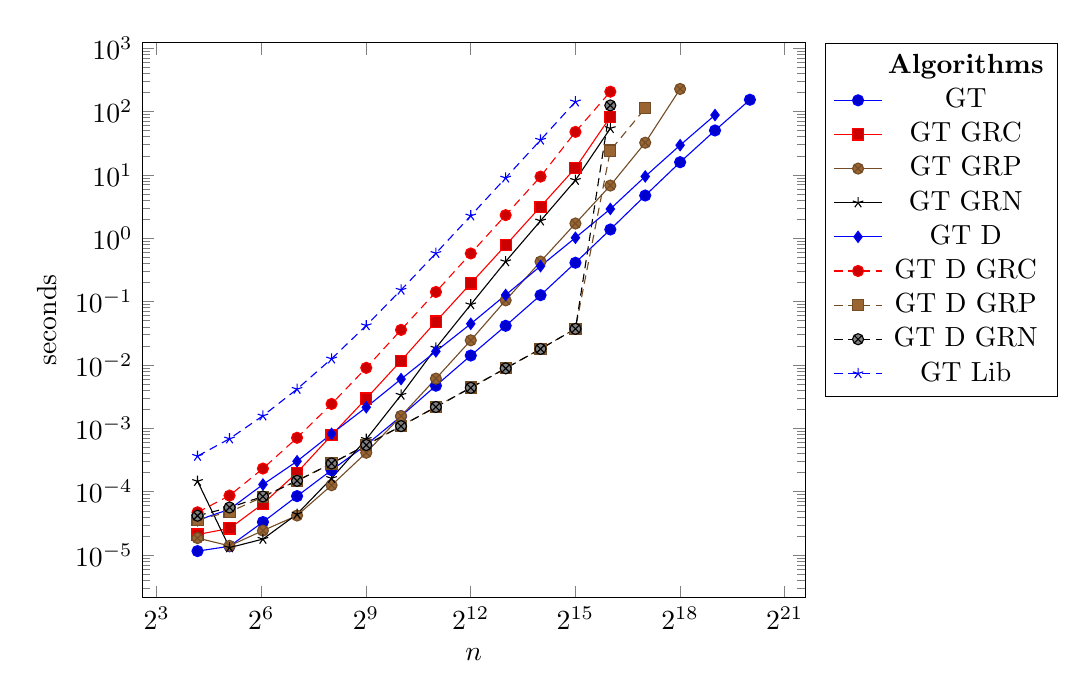
\begin{tikzpicture}
\begin{axis}[
    xlabel=$n$,ylabel=seconds,
    xmode=log,ymode=log,
    log basis x={2},
    legend style=
    {
        legend pos=outer north east
    },
    width=10cm
]
\addlegendimage{legend image code/.code=}
\legend{\textbf{Algorithms}, GT, GT GRC, GT GRP, GT GRN, GT D, GT D GRC, GT D GRP, GT D GRN, GT Lib}
\addplot table[x=n,y=value] {%GT
n value
18	1.15491E-05
34	1.37701E-05
66	3.32038E-05
130	8.51749E-05
258	0.000218989
514	0.000547029
1026	0.001555913
2050	0.004708267
4098	0.014102167
8194	0.041543667
16386	0.126403
32770	0.410714667
65538	1.375183333
131074	4.7243
262146	15.85233333
524290	50.24406667
1048578	153.437
};
\addplot table[x=n,y=value] {%GT GRC
n value
18	2.10994E-05
34	2.63187E-05
66	6.45197E-05
130	0.000200222
258	0.000779344
514	0.002955247
1026	0.011688167
2050	0.0483993
4098	0.193606
8194	0.774928333
16386	3.153233333
32770	12.85786667
65538	82.32676667
};
\addplot table[x=n,y=value] {%GT GRP
n value
18	1.85453E-05
34	1.39922E-05
66	2.43198E-05
130	4.20877E-05
258	0.000126596
514	0.000411993
1026	0.001565127
2050	0.006093057
4098	0.0244856
8194	0.104717
16386	0.428277667
32770	1.70907
65538	6.788133333
131074	32.18266667
262146	227.165
};
\addplot table[x=n,y=value] {%GT GRN
n value
18	0.000146252
34	1.31039E-05
66	0.000017879
130	4.43088E-05
258	0.00016291
514	0.000673739
1026	0.003355143
2050	0.018532733
4098	0.089804633
8194	0.429052667
16386	1.885126667
32770	8.247653333
65538	54.24016667
};
\addplot table[x=n,y=value] {%GT D
n value
18	3.54249E-05
34	5.28596E-05
66	0.000129928
130	0.00030261
258	0.000819102
514	0.002152143
1026	0.005989243
2050	0.016409467
4098	0.044628533
8194	0.127470333
16386	0.363211
32770	1.019396667
65538	2.897966667
131074	9.462753333
262146	29.41903333
524290	88.0256
};
\addplot table[x=n,y=value] {%GT D GRC
n value
18	4.73071E-05
34	8.68408E-05
66	0.000231983
130	0.000709607
258	0.002425103
514	0.009009903
1026	0.0358142
2050	0.142085333
4098	0.575261667
8194	2.315736667
16386	9.388776667
32770	47.68883333
65538	205.5886667
};
\addplot table[x=n,y=value] {%GT D GRP
n value
18	3.60912E-05
34	4.79734E-05
66	8.2621E-05
130	0.000149362
258	0.000279179
514	0.000546364
1026	0.00109295
2050	0.002178017
4098	0.00441367
8194	0.008896857
16386	0.017891767
32770	0.0374025
65538	24.21606667
131074	112.5863333
};
\addplot table[x=n,y=value] {%GT D GRN
n value
18	4.17547E-05
34	5.64132E-05
66	8.40646E-05
130	0.000148473
258	0.000279623
514	0.000545365
1026	0.001084287
2050	0.002170243
4098	0.00436003
8194	0.008836443
16386	0.0179194
32770	0.037174767
65538	124.819
};
\addplot table[x=n,y=value] {%GT Lib
n value
18	0.000364577
34	0.000685067
66	0.001577687
130	0.00415938
258	0.012518467
514	0.0419147
1026	0.152552
2050	0.579812333
4098	2.263826667
8194	8.971396667
16386	35.5501
32770	142.772
};
\end{axis}
\end{tikzpicture}
\caption{Goldberg and Tarjan results from the AK graphs}
\label{fig:AK_GT_Results}
\end{figure}

It is worth noting that we see a similar result for the KR algorithms on the AK graphs in Figure~\ref{fig:AK_KR_Results}. 
Here KR LM D GRN is significantly faster than all others. 
The reason the KR LM D GRP algorithm is slow is explained in Section~\ref{GRP Section}.

We did expect dynamic trees to perform well on the AK graphs, since they feature a very long path that has to be pushed on often. With dynamic trees, this can be done in logarithmic time instead of linear time.
In the other part of the graph however, without global relabelling, it will often push on very short paths which would be more efficient to just do directly. 
With global relabelling, we avoid pushing excess back and forth on these small paths. 
In fact, it creates a longer and longer path that is repeatability pushed on as the algorithm progresses. That is why the algorithm is so fast with heuristics and dynamic trees, but slow with just one of them.
The reason why GT D GRC is performing bad is due to the heuristic trigger, and will be explained in Section~\ref{Global Relabelling Section}.

Our conclusion with regard to dynamic tress is that algorithms only benefit from dynamic trees if the tree pushes mainly push on the same paths repeatability, and the paths are very long.
This generally does not occur, and we only found it in the AK graphs, which are very artificially constructed. On our more randomized graphs like GenRmf and Wash, we saw no improvements by using dynamic trees.

\subsection{Global Relabelling}
\label{Global Relabelling Section}

All of our heuristics perform the same basic global relabelling, but the triggers that determine when to run the global relabelling are different.
Regardless of the trigger, we always run a global relabelling at the start of the algorithm.



\begin{figure}[h]
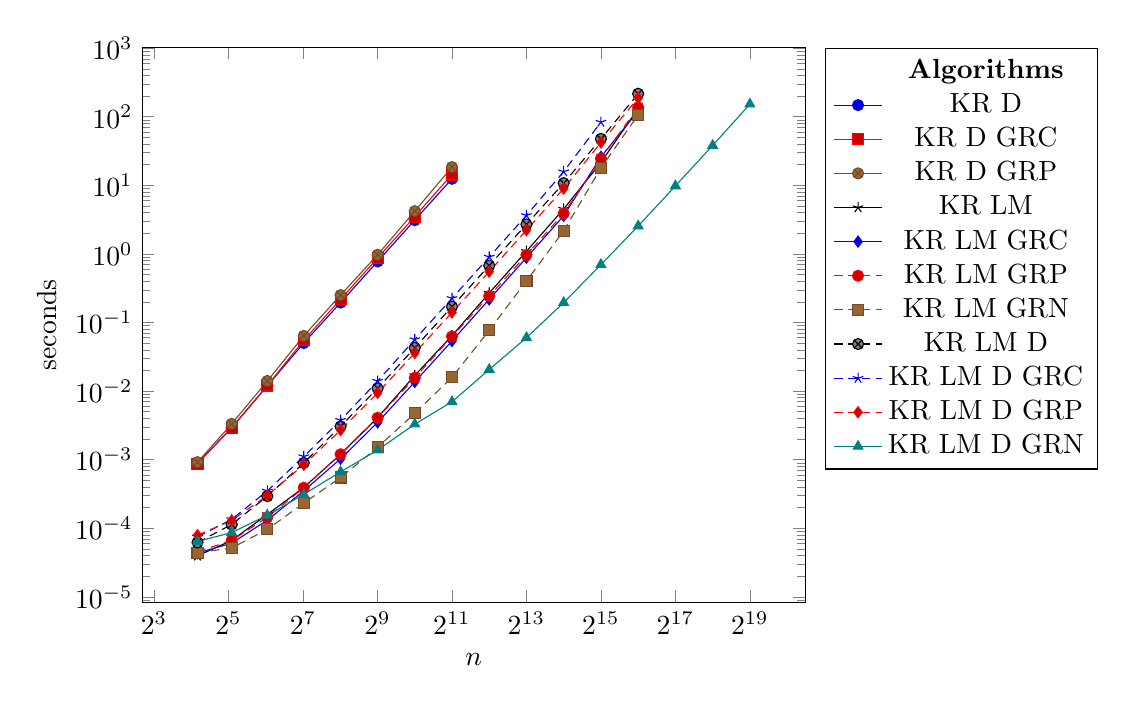
\begin{tikzpicture}
\begin{axis}[
    xlabel=$n$,ylabel=seconds,
    xmode=log,ymode=log,
    log basis x={2},
    legend style=
    {
        legend pos=outer north east
    },
    width=10cm
]
\addlegendimage{legend image code/.code=}
\legend{\textbf{Algorithms}, KR D, KR D GRC, KR D GRP, KR LM, KR LM GRC, KR LM GRP, KR LM GRN, KR LM D, KR LM D GRC, KR LM D GRP, KR LM D GRN}
\addplot table[x=n,y=value] {%KR
n value
18	0.000889175
34	0.002908057
66	0.011943033
130	0.050249867
258	0.195147333
514	0.777756
1026	3.107726667
2050	12.4823
};
\addplot table[x=n,y=value] {%KR GRC
n value
18	0.000875735
34	0.002938147
66	0.0120653
130	0.054935867
258	0.218274
514	0.872710333
1026	3.5095
2050	14.403
};
\addplot table[x=n,y=value] {%KR GRP
n value
18	0.000919492
34	0.00332838
66	0.014040333
130	0.0638248
258	0.251151333
514	0.971965333
1026	4.19931
2050	18.4658
};
\addplot table[x=n,y=value] {%KR LM
n value
18	3.95337E-05
34	6.66298E-05
66	0.000158912
130	0.000393449
258	0.00119856
514	0.00412505
1026	0.016918733
2050	0.064206667
4098	0.268975333
8194	1.09322
16386	4.51368
32770	21.53186667
65538	131.6553333
};
\addplot table[x=n,y=value] {%KR LM GRC
n value
18	4.34204E-05
34	6.07442E-05
66	0.000131261
130	0.000351139
258	0.001029877
514	0.00350173
1026	0.013609367
2050	0.0537659
4098	0.217405
8194	0.881691
16386	3.602213333
32770	26.04033333
65538	120.6886667
};
\addplot table[x=n,y=value] {%KR LM GRP
n value
18	4.57524E-05
34	6.62967E-05
66	0.000144697
130	0.000389451
258	0.00119834
514	0.00407752
1026	0.015643533
2050	0.062576267
4098	0.243189667
8194	0.966999333
16386	3.8901
32770	24.61043333
65538	136.8136667
};
\addplot table[x=n,y=value] {%KR LM GRN
n value
18	4.38646E-05
34	5.16381E-05
66	9.65021E-05
130	0.000232649
258	0.000549696
514	0.00151394
1026	0.00474304
2050	0.0158961
4098	0.0767171
8194	0.402905667
16386	2.16554
32770	17.93576667
65538	106.1156667
};
\addplot table[x=n,y=value] {%KR LM D
n value
18	6.21878E-05
34	0.000113493
66	0.000293837
130	0.000895949
258	0.003054753
514	0.010999333
1026	0.0427871
2050	0.170356
4098	0.676120333
8194	2.693893333
16386	10.74853333
32770	47.54073333
65538	216.514
};
\addplot table[x=n,y=value] {%KR LM D GRC
n value
18	7.48474E-05
34	0.000134814
66	0.000350584
130	0.00111305
258	0.003765693
514	0.014000933
1026	0.0564863
2050	0.225324667
4098	0.904017333
8194	3.646476667
16386	15.8397
32770	83.65686667
};
\addplot table[x=n,y=value] {%KR LM D GRP
n value
18	7.94004E-05
34	0.000130039
66	0.000300056
130	0.000844977
258	0.002696287
514	0.009420677
1026	0.035984667
2050	0.140029
4098	0.551803333
8194	2.21699
16386	8.955463333
32770	42.12056667
65538	186.7876667
};
\addplot[mark=triangle*, teal] table[x=n,y=value] {%KR LM D GRN
n value
18	6.41867E-05
34	8.66187E-05
66	0.00015447
130	0.000312605
258	0.000664521
514	0.001379017
1026	0.003295733
2050	0.006980693
4098	0.020601467
8194	0.0600087
16386	0.194730333
32770	0.69788
65538	2.548136667
131074	9.800743333
262146	38.14566667
524290	152.5736667
};
\end{axis}
\end{tikzpicture}
\caption{King and Rao results from the AK graphs}
\label{fig:AK_KR_Results}
\end{figure}


All of our heuristics perform worse than no heuristics on the CD graphs. This is because it is never needed to send flow back to the source in the CD graph.
None of the global relabels runs relabel any nodes significantly up. 
The AK graphs also do not require any excess to be routed back, but here GT D GRP and GT D GRN are faster than all other GT algorithms.
Likewise, KR LM D GRN is faster than other KR algorithms. This can be seen from Figure~\ref{fig:AK_GT_Results} and Figure~\ref{fig:AK_KR_Results}.
The left side of the AK graphs as depicted in Figure~\ref{akExample} from Section~\ref{AKGraphSection} still cause flow to be pushed back and forth if no global relabelling is done however.


\subsubsection{GRC}

The first heuristic we implemented was the GRC heuristic. It does a global relabelling whenever a node is relabelled more than one label up.
It performs very well on the CRH graphs, but not very well on AK graphs. On GenRmf and Wash graphs, they are more stable than not using heuristics, and generally slightly faster.
The reason we implemented the heuristic was that the running time of the algorithms was very unstable in the GenRmf and Wash graphs, so we did expect the heuristic to be more stable and faster on those graphs.
Examples of the instability in the algorithms without global relabelling can be seen in Figure~\ref{fig:GenRmf long_GT_Results} and Figure~\ref{fig:GenRmf long_KR_Results}.

CRH graphs are the best case graphs for this particular trigger. As soon as the last edge to $t$ is saturated, that node will have to be relabelled twice since all other nodes have a higher label than it does.
That triggers the global relabel, and the excess is then sent to $s$. If you consider the AK graphs however, the square pattern on the left side as depicted in Figure~\ref{akExample} from Section~\ref{AKGraphSection} causes the heuristic to trigger very often.
After the first global relabel, all nodes is labelled according to their distance to $t$. Excess is then pushed from the first node in the lower part of the left side to the top part of the left side and on to $t$.
For the algorithm to continue here, excess must be pushed to the next node in the lower part of the left side. This requires that the first node in the lower part is relabelled twice, even though nothing has been pushed in a cycle.
The global relabel is not going to change any labels on the left side, so it is just wasted effort.
This happens again and again each time flow is pushed further along the lower part of the left side.
The performance on CRH and AK graphs can be seen in Appendix~\ref{ChartAppendix}.

This triggering of the heuristic when there are no cycles is why we decided to implement the GRP trigger.

\subsubsection{GRP}
\label{GRP Section}

The GRP trigger triggers when flow has not been sent to the target since the last pass, if flow has been sent to the target since the last global relabelling.
This gave a major speed-up for the GT algorithms on GenRmf and Wash graphs. This can for instance be seen in Figure~\ref{fig:GenRmf square_GT_Results}. 
As discussed in Section~\ref{Dynamic Trees Section}, GT D GRP gained major speed-ups on the AK graphs as well.

As can be seen from Figure~\ref{fig:GenRmf long_KR_Results}, we did not see any major speed-ups for the KR algorithms when using the GRP heuristic instead of the GRC heuristic. 
Due to the way edges are added in the KR algorithm, there are not many active nodes at a time in the KR algorithm.
When an edge $(u, v)$ is added, it might cause the visible excess of $u$ become positive and activate the node.
This causes the excess to be pushed around the graph, which might activate other nodes.
The number of nodes that are active at the same time remain low though, which means the global relabelling check is called very often.
A result of this is that the KR algorithms with the GRP heuristic perform a global relabel every time the excess of $t$ changes.

To get a more consistent speed-up, we decided to base the trigger off the number of nodes processed instead of passes, which lead to the GRN heuristic.

\subsubsection{GRN}

Instead of checking the excess of $t$ after each pass, the GRN heuristic does it after $f(G)$ nodes have been processed.
This improved upon the running times for the GT and KR algorithms on the AK, GenRmf and Wash graphs.
For examples of this, see Figures 
\ref{fig:GenRmf long_GT_Results}, 
\ref{fig:GenRmf long_KR_Results}, 
\ref{fig:GenRmf square_GT_Results}, 
\ref{fig:AK_GT_Results}, 
\ref{fig:AK_KR_Results}, 
or Appendix~\ref{ChartAppendix}.

\subsection{Library Implementations}

We tested a set of max flow algorithms from the C++ Boost Library \cite{BoostLibraries}.
It has implementations for the Edmonds and Karp algorithm, the Goldberg and Tarjan algorithm, and an algorithm by Boykov and Kolmogorov.
The Boykov and Kolmogorov algorithm is an algorithm that is designed to be efficient on a special type of max flow graphs that arise from computer vision.

We tested the algorithms on all of our graphs, and found that the library algorithms are relatively slow.
The library implementation of the Edmonds and Karp algorithm is almost 100 times slower than our implementation, even though we have not done any significant optimizations to it.
The implementation of the Goldberg and Tarjan algorithm is also slow compared to our implementations. 
If you look at Figure~\ref{fig:GenRmf square_GT_Results}, you can see that GT Lib is about the same time as our implementations without heuristics or with the GRC heuristic.
It is slower for small graphs, and faster for larger graphs. The slope is about the same as our algorithms with the GRN heuristic, but it is again about 100 times slower.
The slope and lack of jumps tell us that they do use some form of heuristics to detect when the min cut is saturated.
We have profiled it to ensure that it is not something in our code that is causing the slowdown, but all the work is done in functions inside the boost library.

As for the BK Lib algorithm, if we compare it to GT Lib, then BK Lib is faster on small graphs, and GT tends to win as the graphs become bigger.
It is still far behind our best algorithms on all graphs.


\begin{figure}[h]
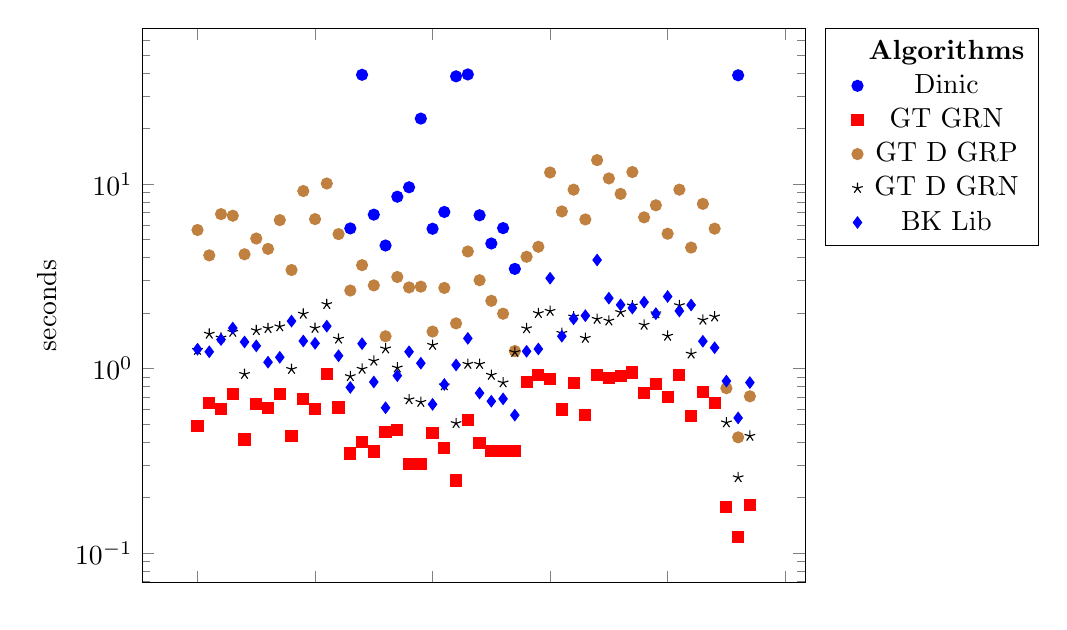
\begin{tikzpicture}
\begin{axis}[
    ylabel=seconds,ymode=log,
	symbolic x coords={BVZ-sawtooth04,BVZ-sawtooth06,BVZ-sawtooth07,BVZ-sawtooth08,BVZ-sawtooth09,BVZ-sawtooth10,BVZ-sawtooth11,BVZ-sawtooth12,BVZ-sawtooth13,BVZ-sawtooth14,BVZ-sawtooth15,BVZ-sawtooth16,BVZ-sawtooth18,BVZ-tsukuba00,BVZ-tsukuba01,BVZ-tsukuba02,BVZ-tsukuba03,BVZ-tsukuba04,BVZ-tsukuba05,BVZ-tsukuba6,BVZ-tsukuba7,BVZ-tsukuba8,BVZ-tsukuba9,BVZ-tsukuba10,BVZ-tsukuba11,BVZ-tsukuba12,BVZ-tsukuba14,BVZ-tsukuba15,BVZ-venus01,BVZ-venus02,BVZ-venus03,BVZ-venus04,BVZ-venus05,BVZ-venus06,BVZ-venus07,BVZ-venus08,BVZ-venus09,BVZ-venus10,BVZ-venus11,BVZ-venus12,BVZ-venus13,BVZ-venus14,BVZ-venus15,BVZ-venus16,BVZ-venus17,KZ2-sawtooth17,KZ2-tsukuba13,KZ2-venus19},
	xticklabels={,,},
    legend style=
    {
        legend pos=outer north east
    },
    width=10cm
]
\addlegendimage{legend image code/.code=}
\legend{\textbf{Algorithms}, Dinic, GT GRN, GT D GRP, GT D GRN, BK Lib}
\addplot[only marks, blue, mark=*] table[x=n,y=value] {%Dinic
n value
BVZ-tsukuba00	5.750836667
BVZ-tsukuba01	39.14823333
BVZ-tsukuba02	6.83006
BVZ-tsukuba03	4.645143333
BVZ-tsukuba04	8.541403333
BVZ-tsukuba05	9.609163333
BVZ-tsukuba10	39.3178
BVZ-tsukuba11	6.7765
BVZ-tsukuba12	4.763366667
BVZ-tsukuba14	5.771553333
BVZ-tsukuba15	3.468896667
BVZ-tsukuba6	22.6535
BVZ-tsukuba7	5.724696667
BVZ-tsukuba8	7.061796667
BVZ-tsukuba9	38.3952
KZ2-tsukuba13	38.90546667
};
\addplot[only marks, red, mark=square*] table[x=n,y=value] {%GT GRN
n value
BVZ-sawtooth04	0.489767333
BVZ-sawtooth06	0.650722667
BVZ-sawtooth07	0.602036667
BVZ-sawtooth08	0.728916
BVZ-sawtooth09	0.412417333
BVZ-sawtooth10	0.642597
BVZ-sawtooth11	0.610116
BVZ-sawtooth12	0.731337
BVZ-sawtooth13	0.429253333
BVZ-sawtooth14	0.683659333
BVZ-sawtooth15	0.604143
BVZ-sawtooth16	0.933819
BVZ-sawtooth18	0.614827667
BVZ-tsukuba00	0.346019
BVZ-tsukuba01	0.39826
BVZ-tsukuba02	0.355036667
BVZ-tsukuba03	0.452382667
BVZ-tsukuba04	0.462989667
BVZ-tsukuba05	0.302774
BVZ-tsukuba10	0.523340333
BVZ-tsukuba11	0.394437667
BVZ-tsukuba12	0.357265333
BVZ-tsukuba14	0.356760667
BVZ-tsukuba15	0.358245
BVZ-tsukuba6	0.30229
BVZ-tsukuba7	0.447588333
BVZ-tsukuba8	0.371264
BVZ-tsukuba9	0.247241333
BVZ-venus01	0.844272667
BVZ-venus02	0.918598
BVZ-venus03	0.873629667
BVZ-venus04	0.599272
BVZ-venus05	0.836556333
BVZ-venus06	0.559744667
BVZ-venus07	0.920171667
BVZ-venus08	0.885694
BVZ-venus09	0.912648
BVZ-venus10	0.951088333
BVZ-venus11	0.740437333
BVZ-venus12	0.821746
BVZ-venus13	0.702746333
BVZ-venus14	0.926211
BVZ-venus15	0.550986667
BVZ-venus16	0.742330333
BVZ-venus17	0.649391333
KZ2-sawtooth17	0.177902
KZ2-tsukuba13	0.12262
KZ2-venus19	0.181196667
};
\addplot[only marks, brown, mark=oplus*] table[x=n,y=value] {%GT D GRP
n value
BVZ-sawtooth04	5.637843333
BVZ-sawtooth06	4.106903333
BVZ-sawtooth07	6.87372
BVZ-sawtooth08	6.738953333
BVZ-sawtooth09	4.163056667
BVZ-sawtooth10	5.067443333
BVZ-sawtooth11	4.45305
BVZ-sawtooth12	6.378663333
BVZ-sawtooth13	3.42055
BVZ-sawtooth14	9.17015
BVZ-sawtooth15	6.45878
BVZ-sawtooth16	10.07306667
BVZ-sawtooth18	5.355506667
BVZ-tsukuba00	2.647463333
BVZ-tsukuba01	3.635553333
BVZ-tsukuba02	2.823506667
BVZ-tsukuba03	1.495733333
BVZ-tsukuba04	3.1349
BVZ-tsukuba05	2.75291
BVZ-tsukuba10	4.310993333
BVZ-tsukuba11	3.01142
BVZ-tsukuba12	2.328253333
BVZ-tsukuba14	1.98249
BVZ-tsukuba15	1.243746667
BVZ-tsukuba6	2.779606667
BVZ-tsukuba7	1.58586
BVZ-tsukuba8	2.73537
BVZ-tsukuba9	1.757243333
BVZ-venus01	4.034523333
BVZ-venus02	4.57276
BVZ-venus03	11.55953333
BVZ-venus04	7.10882
BVZ-venus05	9.328716667
BVZ-venus06	6.432303333
BVZ-venus07	13.49126667
BVZ-venus08	10.73153333
BVZ-venus09	8.848846667
BVZ-venus10	11.6229
BVZ-venus11	6.6005
BVZ-venus12	7.675843333
BVZ-venus13	5.381833333
BVZ-venus14	9.32988
BVZ-venus15	4.527093333
BVZ-venus16	7.814476667
BVZ-venus17	5.7328
KZ2-sawtooth17	0.782533333
KZ2-tsukuba13	0.42346
KZ2-venus19	0.706977667
};
\addplot[only marks, black, mark=star] table[x=n,y=value] {%GT D GRN
n value
BVZ-sawtooth04	1.257363333
BVZ-sawtooth06	1.5395
BVZ-sawtooth07	1.467783333
BVZ-sawtooth08	1.575723333
BVZ-sawtooth09	0.931440667
BVZ-sawtooth10	1.60887
BVZ-sawtooth11	1.65183
BVZ-sawtooth12	1.687383333
BVZ-sawtooth13	0.991900333
BVZ-sawtooth14	1.97617
BVZ-sawtooth15	1.65473
BVZ-sawtooth16	2.2296
BVZ-sawtooth18	1.4468
BVZ-tsukuba00	0.906884333
BVZ-tsukuba01	0.993645333
BVZ-tsukuba02	1.099296667
BVZ-tsukuba03	1.280756667
BVZ-tsukuba04	1.009479333
BVZ-tsukuba05	0.679007
BVZ-tsukuba10	1.05689
BVZ-tsukuba11	1.0557
BVZ-tsukuba12	0.921605
BVZ-tsukuba14	0.837999333
BVZ-tsukuba15	1.225756667
BVZ-tsukuba6	0.657387333
BVZ-tsukuba7	1.33941
BVZ-tsukuba8	0.807863333
BVZ-tsukuba9	0.504580667
BVZ-venus01	1.648326667
BVZ-venus02	1.992683333
BVZ-venus03	2.047933333
BVZ-venus04	1.555906667
BVZ-venus05	1.909363333
BVZ-venus06	1.461823333
BVZ-venus07	1.853596667
BVZ-venus08	1.81487
BVZ-venus09	2.017216667
BVZ-venus10	2.190356667
BVZ-venus11	1.721903333
BVZ-venus12	1.98797
BVZ-venus13	1.501023333
BVZ-venus14	2.19958
BVZ-venus15	1.20103
BVZ-venus16	1.834053333
BVZ-venus17	1.909196667
KZ2-sawtooth17	0.508664
KZ2-tsukuba13	0.256661
KZ2-venus19	0.430539333
};
\addplot[only marks, blue, mark=diamond*] table[x=n,y=value] {%BK Lib
n value
BVZ-sawtooth04	1.272543333
BVZ-sawtooth06	1.23261
BVZ-sawtooth07	1.43546
BVZ-sawtooth08	1.65753
BVZ-sawtooth09	1.39307
BVZ-sawtooth10	1.32683
BVZ-sawtooth11	1.082433333
BVZ-sawtooth12	1.150216667
BVZ-sawtooth13	1.807283333
BVZ-sawtooth14	1.409916667
BVZ-sawtooth15	1.36928
BVZ-sawtooth16	1.69699
BVZ-sawtooth18	1.172643333
BVZ-tsukuba00	0.789907667
BVZ-tsukuba01	1.363463333
BVZ-tsukuba02	0.844900667
BVZ-tsukuba03	0.612848667
BVZ-tsukuba04	0.914284667
BVZ-tsukuba05	1.232753333
BVZ-tsukuba10	1.457013333
BVZ-tsukuba11	0.736029333
BVZ-tsukuba12	0.664695333
BVZ-tsukuba14	0.684720333
BVZ-tsukuba15	0.559057667
BVZ-tsukuba6	1.068726667
BVZ-tsukuba7	0.639465
BVZ-tsukuba8	0.819790667
BVZ-tsukuba9	1.045543333
BVZ-venus01	1.240246667
BVZ-venus02	1.27637
BVZ-venus03	3.08739
BVZ-venus04	1.497496667
BVZ-venus05	1.8612
BVZ-venus06	1.934973333
BVZ-venus07	3.87581
BVZ-venus08	2.406416667
BVZ-venus09	2.214203333
BVZ-venus10	2.129076667
BVZ-venus11	2.290323333
BVZ-venus12	1.983696667
BVZ-venus13	2.456886667
BVZ-venus14	2.050246667
BVZ-venus15	2.21068
BVZ-venus16	1.405656667
BVZ-venus17	1.296033333
KZ2-sawtooth17	0.855298667
KZ2-tsukuba13	0.539781667
KZ2-venus19	0.839086
};
\end{axis}
\end{tikzpicture}
\caption{Results from the Computer Vision graphs}
\label{fig:CV_Results}
\end{figure}

To get some graphs that BK Lib should work well on, we found some max flow graphs that are generated from computer vision problems \cite{CVGraphsSite}.
The graphs are rather big, so we have not been able to run all of our algorithms on them, but GT GRN, GT D GRP, GT D GRN and BK Lib all perform well enough for us to get data on them within reasonable time.
The data for the CV graphs can be seen in Figure~\ref{fig:CV_Results}.
When we ran the tests, we ran each algorithms on the graphs for 15 minutes. The order the graphs were tested was sorted by file size on disk, 
but in in Figure~\ref{fig:CV_Results} the points are alphabetically sorted.
From left to right, the chart contains data for BVZ-sawtooth number 4, 6-16 and 18, BVZ-tsukuba number 0-15, BVZ-venus number 1-17, and the graphs KZ2-sawtooth17, KZ2-tsukuba13 and KZ2-venus19.

As expected, the BK Lib algorithm performs quite well on these graphs.
It is not fast enough to beat GT GRN, but it is the second fastest algorithm we have tested.

\section{Future Works}
If we had more time, we would have liked to spend more time optimizing our algorithms.
We believe that there is still room for improvements in experimenting with some of the parameters in the algorithms.

Also, better algorithms for routing the blocking flow in Dinic might speed up this algorithm.
A problem with Dinic right now is that it might process the same part of the layer graph multiple times.
It might be possible to speed it up by saving information about the paths in the layer graph that has already been visited once.
One way of doing this could be using dynamic trees, but we have not seen a big improvement for the other algorithms when using dynamic trees.
That having been said, layer graphs does tend to be long paths with reusable edges, so we could see a good performance boost by adding dynamic trees.
Alternatively, we could use the push pull block algorithm that is used in Goldberg Rao to compute the blocking flow, which would also reduce the theoretical running time to $O\left(nm\log{\frac{n^2}{m}}\right)$.

As mentioned in Section~\ref{ImplementationSection}, we could probably gain some performance by using templates for custom data in nodes instead of a pointer to an object containing the custom data.
A graph node takes up 24 bytes, and an edge takes 32 bytes. With a cache line of 64 bytes, this means we load about two nodes with every cache miss.
The probability that we need the other node is low however as proximity in memory does not imply proximity in the graph.
Even if the first node has an edge to the other node, it probably has edges to other nodes as well.
In the table below we listed the sizes for some of the objects in our algorithms.
\begin{table}[h]
\centering
\begin{tabular}{|l|r|r|}
\hline
\multicolumn{1}{|l}{Object} &
\multicolumn{1}{|l}{Size} &
\multicolumn{1}{|l|}{Padding} \\\hline
Node&24 bytes & 4 bytes\\\hline
Edge&32 bytes & 4 bytes\\\hline
EK Node Tag & 16 bytes & 0 bytes\\\hline
Dinic Node Tag & 24 bytes & 0 bytes\\\hline
GT Node Tag & 24 bytes & 4 bytes\\\hline
GT D Node Tag & 32 bytes & 4 bytes\\\hline
KR LM Node Tag & 128 bytes & 4 bytes\\\hline
Dynamic Tree Node & 80 bytes & 0 bytes\\\hline
\end{tabular}
\end{table}\\
Variables are aligned to start on an address that is a multiple of their size. For instance, a 4 byte variable can start on address $4, 8, 12$ etc.
Variables are aligned by padding the previous variable. For instance, if we define a 32 bit variable followed by a 64 bit variable, 
the 32 bit variable will be padded to 64 bit so the 64 bit variable starts at a multiple of 8.
To allow putting structs next to each other in an array, the struct is also padded so that its size is a multiple of the size of the biggest primitive in it.
For instance, we use 64 bit pointers, which means that any struct that contains a pointer is padded so that its size in bytes is a multiple of 8.
Padding to align variables can generally be avoided by defining them in order of biggest to smallest.
The size column specifies the total size of the object, and the padding column specifies how much of that is padding. 
This means that if we were to merge two objects each of size 24 bytes with 4 bytes of padding, we would be able to merge those to an object of size 40 bytes with no padding.
Additionally, merging a tag with the node removes the need for the pointer in the node to the tag.

What is interesting about this table is that node tags from all algorithms except from KR can be merged with the graph node into an object that fits into one cache line.
In fact, merging GT results in an object that takes up 24 bytes from the node, 24 bytes from the GT tag, minus 8 bytes from padding, and minus 8 bytes for one less pointer in the node.
In total, 32 bytes. That means that two nodes would fit perfectly into one cache line. 
We went up to 64 bit pointers due to memory issues in KR, but with 32 bit pointers, a merged graph node and GT D node tag would take up 28 bytes.
This would also allow for GT D to place two merged nodes in one cache line.
Since 28 bytes is not a perfect half cache line though, $1/4$ of the nodes will be placed to span two cache lines.
It might be worth it to pad these nodes with an extra 4 bytes so that no nodes span two cache lines.

The KR tags take up a lot of memory because they need to contain the game in them, which means a lot of linked lists.
This means that we would not be able to read an entire node in one cache line, but we would still expect to see a performance increase.
The reason is that the CPU could load the information it needs directly instead of having to load a pointer and then load the information it needs.

As mentioned before, the downside of this optimization is that the graph needs to be cloned. 
For graphs such as CRE and CRH, that is probably not worth it due to the large number of edges that do not need to be used, but we would expect to see a speed up on our other graphs.

We have not had much time to optimize the Goldberg Rao algorithm, so more work on that could bring its running time down.

Finally, it would be interesting to implement Orlin and compare it to the other algorithms. 
We don't expect it will be faster though, since it adds a lot of complexity and memory use.

\section{Conclusion}

Although we did not get to implementing the Orlin algorithm \cite{Orlin13} as we had hoped, we did get some interesting results.
Our contribution to the algorithm by King and Rao is not only a theoretical result, but it also makes a big difference in practice.
The addition to the Goldberg Rao theory fixes an issue it has with one of its assumptions, and make the theory hold.

On the performance side of things, we can conclude that a naive implementation of the algorithm by Dinic is often better than a naive implementation of the other algorithms.
However, we found more room for optimizations and heuristics on the Push-Relabel algorithms such as the algorithms by Goldberg and Tarjan, and by King and Rao.
We did not find the added complexity of the King Rao algorithms in relation to the Goldberg Tarjan algorithms to be worth it however.
Likewise, the algorithms do for the most part not benefit from dynamic trees.
It appears as though the Goldberg Rao algorithm has too many different things going on for it to be really efficient, but there is room for optimizations in our implementation.


























































\settocdepth{section}
\clearpage

\bibliography{mybib}{}
%\bibliographystyle{plain}
\bibliographystyle{alpha}




\newpage
\appendix 
\begin{subappendices}

\section{Terminology Tables}
\label{TerminologyAppendix}

\subsection{Section \ref{TerminologySection}: General Terminology}
\makebox[\textwidth][c]{
\begin{tabular}{ l l l }
Name & Symbol & Short Description\\
\hline 
Graph & $G$ & \\
Node set & $V$ & \\
Edge set & $E$ & \\
Path & $(v_1, \cdots , v_k)$ & List of nodes connected by edges \\
Residual path &  & A path where all edges have $r(u, v) > 0$ \\
Augmenting path &  & A residual path from $s$ to $t$ \\
Bounding edge &  & The edges in a residual path that have  \\
&&minimum residual capacity\\
Capacity & $cap(u, v)$ & Maximum flow that can be sent on an edge \\
Maximum capacity & $U$ & $\max\limits_{(u, v)\in E}cap(u, v)$ \\
Flow & $f(u, v)$ & The flow sent on an edge \\
Residual capacity& $r(u, v)$ & The amount of flow that can be sent \\
&&without exceeding $cap$\\
Residual Edge & & An edge where the residual capacity replaces the capacity\\
Edge set & $E_f$ & The set of residual edges of $E$ based on flow $f$\\
Residual Graph &$G_f$& $G_f = (V,E_f)$\\
An Eligeble edge & & Has positive residual capacity\\
Saturated edge& & An edge where $r(u, v) = 0$ \\
Distance& $distance(u, v)$ & Number of edges in the shortest \\
&&residual path connecting $u$ to $v$\\
Excess & $e(v)$ & The sum of flow entering a node $v$, \\
&&minus the sum of flow exiting it.\\
\hline
\end{tabular}
}

\subsection{Section \ref{ParadigmsSection}: Paradigms}
\makebox[\textwidth][c]{
\begin{tabular}{ l l l }
Name & Symbol & Short Description\\
\hline 
Blocking flow & &\\
Layer Graph  & &\\
Push, Relabel  & &\\
Label  & $d(v)$ & The label of a node $v$. Used by Push-Relable algorithms.\\
\hline
\end{tabular}
}

\subsection{Section \ref{GoldbergTarjanSection}: A. V. Goldberg R. E. Tarjan 1988}
\makebox[\textwidth][c]{
\begin{tabular}{ l l }
Symbol & Short Description\\
\hline 
Eligible & An edge $(v,w)$ is eligible if it has $r(v,w) > 0$\\
Active & A node $v$ is active if $e(v) > 0$\\
Current-edge & The edge the algorithm would try to push on next. \\
&Also the edge linked in the Dynamic Tree data structure\\
Saturating push & A push operation on an edge that used all the residual capacity \\
Pass & Pass $i+1$ consist of working on all the nodes that was put in the queue at pass $i$\\
Large & A dynamic tree $T$ is large if $|T| \geq k/2$\\
\hline
\end{tabular}
}

\subsection{Section \ref{KRGameSection}: King Rao 1992 - The Game}
\makebox[\textwidth][c]{
\begin{tabular}{ l l }
Symbol & Short Description\\
\hline 
$G_g=(U_g, V_g, E_g)$ & A bipartite graph used in the game\\
$N=|U_g|=|V_g|$ & The number of nodes in the game graph.\\
$M=|E_g|$ & The number of edges in the game graph.\\
$P(N, M)$ & A function that specifies a bound on how   \\
& many points the adversary can obtain.\\
$C(N, M)$ & A function that specifies a bound on the \\
& cost of implementing the player's strategy.\\
$r_0$ & Determines when a node changes ratio level.\\
$r_i=2^ir_0$ & \\
$t$ & The highest ratio level allowed is $r_t$.\\
$l$ & Nodes with fewer edges than the parameter $l$\\
& can use any edge as the designated edge.\\
$U_g'=\{u \in U_g \mid \mathrm{degree}(u) > l\}$ & The nodes in $U_g$ that has degree greater than $l$.\\
$r(v)=\frac{\mathrm{degree_{designated}}(v)}{\mathrm{degree_{initial}}(v)}$ & The ratio of the node $v \in V_g$.\\
$rl(v)=\left\{
\begin{aligned}
0 &\text{ if }r(v)<r_0\\
i &\text{ if }r_i \leq r(v)< r_{i+1}\\
t &\text{ if }r_t \leq r(v)
\end{aligned}
\right.$ & The ratio level of the node $v \in V_g$.\\
$erl(v)\in [rl(v), rl(v)+1]$ & The estimated ratio level of the node $v \in V_g$\\
$V_i=\left\{v\in V_g\mid rl(v) \geq i\right\}$ & \\
$U_i$ & Nodes in $U_g'$ whose designated edge go to a node in $V_i$. \\
\hline
\end{tabular}
}

\subsection{Section \ref{KRGameAnalysisSection}: King Rao 1992 - Analysis of The Game}
\makebox[\textwidth][c]{
\begin{tabular}{ l l }
Symbol & Short Description\\
\hline 
$U_i(v)$ & The nodes in $U_i$ whose designated edge go to $v$.\\
\hline
\end{tabular}
}

\subsection{Section \ref{KRAlgorithmSection}: King Rao 1992 - The Algorithm}
\makebox[\textwidth][c]{
\begin{tabular}{ l l }
Symbol & Short Description\\
\hline 
$E^*\subseteq E$ & The edges that are added to the graph\\
$h(v)=\sum\limits_{(v, u)\in E\setminus E^*}{cap(v, u)}$ & The hidden capacity of a node.\\
$e^*(v)=max\left(0, e(v)-h(v)\right)$ & The visible excess of a node. A node is not allowed to\\
& push more flow away from it than its visible excess.\\
\hline
\end{tabular}
}

\subsection{Section \ref{GRSection}: A. V. Goldberg S. Rao 1998}
\makebox[\textwidth][c]{
\begin{tabular}{ l l }
Symbol & Short Description\\
\hline 
$\Lambda = \min{\{n^{\frac{2}{3}},m^{\frac{1}{2}}\}}$ & \\
$\Delta=\frac{F}{\Lambda}$ & Bounds which edges are admissible\\
$d(v)$ & The distance label of a node $v$\\
$ l(v,w)$ & Length function. Zero iff $r(v,w) \geq 2\Delta$\\
Special edge $(v,w)$ & $\Delta \leq r(v,w) \leq 2\Delta, d(v) = d(w), r(w,v) \geq 2\Delta$\\
$ \bar{l}(v,w)$ & Length function. Zero if special edge or $r(v,w) \geq 2\Delta$\\
Admissible & An edge $(v,w)$ is admissible if $d(v) = \bar{l}(v,w) + d(w)$ and $r(v,w)>0$\\
$F$ & Upper bound on the remaining flow that can be sent.\\
 & It is updated to capacities of cuts in the graph.\\
Iteration & One iteration is one sequence of constructing a layer graph,\\
& running the blocking flow algorithm and routing flow in SSCs.\\
Phase & One phase is a series of iterations resulting in an update to $F$\\
\hline
\end{tabular}
}


\subsection{Algorithm Abbriviations}
\label{AlgorithmAbbrivationsSection}
\makebox[\textwidth][c]{
\begin{tabular}{|l|c|c|c|c|}
    Abbriviation & Dynamic Trees & Low Memory & Global Relabeling Trigger & Library \\\hline\hline
    \multicolumn{5}{|c|}{\textbf{Edmonds and Karp}} \\\hline
    EK &&&&\\\hline
    EK Lib&&&&$\times$\\\hline\hline
    \multicolumn{5}{|c|}{\textbf{Dinic}} \\\hline
    Dinic &&&&\\\hline\hline
    \multicolumn{5}{|c|}{\textbf{Goldberg and Tarjan}} \\\hline
    GT &&&&\\\hline
    GT GRC &&&Cycle&\\\hline
    GT GRP &&&Pass&\\\hline
    GT GRN &&&Node Count&\\\hline
    GT D&$\times$&&&\\\hline
    GT D GRC &$\times$&&Cycle&\\\hline
    GT D GRP &$\times$&&Pass&\\\hline
    GT D GRN &$\times$&&Node Count&\\\hline
    GT Lib&&&&$\times$\\\hline\hline
    \multicolumn{5}{|c|}{\textbf{King and Rao}} \\\hline
    KR D&$\times$&&&\\\hline
    KR D GRC&$\times$&&Cycle&\\\hline
    KR D GRP&$\times$&&Pass&\\\hline
    KR LM&&$\times$&&\\\hline
    KR LM GRC&&$\times$&Cycle&\\\hline
    KR LM GRP&&$\times$&Pass&\\\hline
    KR LM GRN&&$\times$&Node Count&\\\hline
    KR LM D&$\times$&$\times$&&\\\hline
    KR LM D GRC&$\times$&$\times$&Cycle&\\\hline
    KR LM D GRP&$\times$&$\times$&Pass&\\\hline
    KR LM D GRN&$\times$&$\times$&Node Count&\\\hline\hline
    \multicolumn{5}{|c|}{\textbf{Goldberg and Rao}} \\\hline
    GR&$\times$&&&\\\hline\hline
    \multicolumn{5}{|c|}{\textbf{Boykov and Kolmogorov}} \\\hline
    BK Lib&&&&$\times$\\\hline
\end{tabular}
}


\subsection{Global Relabeling Node count trigger functions}
\label{GRN_Functions}
\makebox[\textwidth][c]{
\begin{tabular}{|l|c|c|}
    \hline
    Algorithm & Function & $R^2$ \\\hline\hline
    GT GRN&$f(G)=2.018n^{0.6488}$&$0.946$\\\hline
    GT D GRN&$f(G)=0.5281n^{0.7145}$&$0.9325$\\\hline
    KR LM GRN&$f(G)=2.1674n^{0.7244}$&$0.7766$\\\hline
    KR LM D GRN&$f(G)=11.649n^{0.4249}$&$0.1684$\\\hline
\end{tabular}
}

\begin{figure}[h]
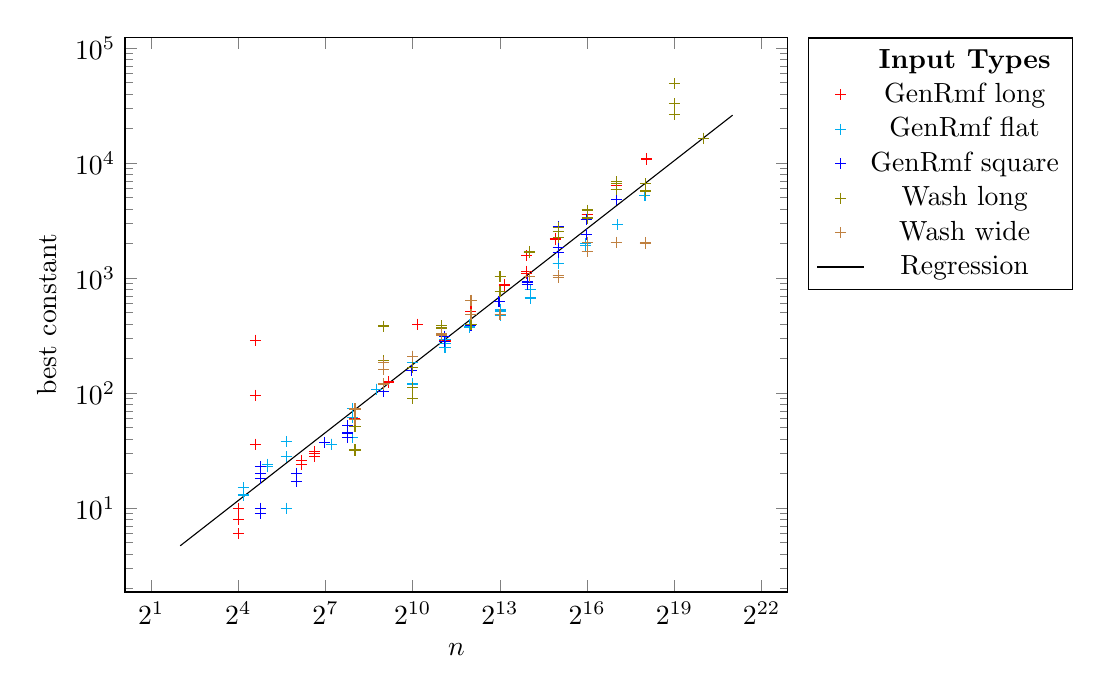
\begin{tikzpicture}
\begin{axis}[
    xlabel=$n$,ylabel=best constant,
    xmode=log,ymode=log,
    log basis x={2},
    legend style=
    {
        legend pos=outer north east
    },
    width=10cm
]
\addlegendimage{legend image code/.code=}
\legend{\textbf{Input Types}, GenRmf long, GenRmf flat, GenRmf square, Wash long, Wash wide, Regression}
\addplot [mark=+, red, only marks]table[x=n,y=value] {%GenRmf long
n   value
16	6
24	96
72	26
99	31
256	60
575	123
1152	396
2205	284
4096	512
9100	864
15488	1565
30589	2206
65536	3584
130682	5869
270848	10712
16	10
24	36
72	24
99	28
256	60
575	125
1152	396
2205	284
4096	512
9100	878
15488	1149
30589	2149
65536	3584
130682	6380
270848	10712
16	8
24	289
72	24
99	30
256	60
575	125
1152	396
2205	281
4096	512
9100	868
15488	1089
30589	2206
65536	3584
130682	5901
270848	10922
};
\addplot [mark=+, cyan, only marks]table[x=n,y=value] {%GenRmf flat
n   value
18	15
32	23
50	28
147	36
243	41
432	108
1024	184
2205	292
3920	380
8214	517
16807	795
32768	1344
63504	1937
135531	2908
259308	5218
18	13
32	24
50	38
147	36
243	61
432	108
1024	120
2205	272
3920	374
8214	533
16807	795
32768	1344
63504	1987
135531	2908
259308	5218
18	15
32	24
50	10
147	36
243	73
432	108
1024	184
2205	250
3920	397
8214	476
16807	671
32768	1344
63504	1987
135531	2908
};
\addplot [mark=+, blue, only marks]table[x=n,y=value] {%GenRmf square
n   value
27	20
27	23
64	20
125	37
216	52
512	104
1000	156
2197	309
4096	385
8000	625
15625	884
32768	1841
64000	3234
132651	4789
27	9
27	9
64	17
125	37
216	41
512	104
1000	156
2197	312
4096	384
8000	625
15625	933
32768	1680
64000	3234
132651	4792
27	10
27	18
64	20
125	37
216	45
512	104
1000	156
2197	282
4096	384
8000	625
15625	916
32768	2816
64000	2375
132651	4792
};
\addplot [mark=+, olive, only marks]table[x=n,y=value] {%Wash long
n   value
258	32
514	192
1026	168
2050	368
4098	480
8194	1024
16386	1673
32770	2752
65538	3344
131074	6880
262146	6592
524290	32768
1048578	16384
258	51
514	191
1026	112
2050	368
4098	480
8194	768
16386	1707
32770	2536
65538	3909
131074	5887
262146	5631
524290	49152
1048578	16512
258	32
514	383
1026	90
2050	384
4098	392
8194	1028
16386	1664
32770	2268
65538	3328
131074	6646
262146	5744
524290	26640
1048578	16512
};
\addplot [mark=+, brown, only marks]table[x=n,y=value] {%Wash wide
n   value
258	73
514	120
1026	209
2050	325
4098	480
8194	481
16386	1024
32770	1052
65538	2046
131074	2048
262146	1984
258	72
514	160
1026	209
2050	316
4098	480
8194	480
16386	1026
32770	1052
65538	1696
131074	2048
262146	1984
258	59
514	184
1026	209
2050	328
4098	640
8194	480
16386	1024
32770	1016
65538	1696
131074	2048
262146	2048
};
\addplot [domain=4:2097152]{1.8956*x^0.6548};
\end{axis}
\end{tikzpicture}
\caption{Constant estimation for Global Relabel with node count trigger for Goldberg Tarjan (GT GRN)}
\label{fig:GT_GRN_Constant}
\end{figure}

\begin{figure}[h]
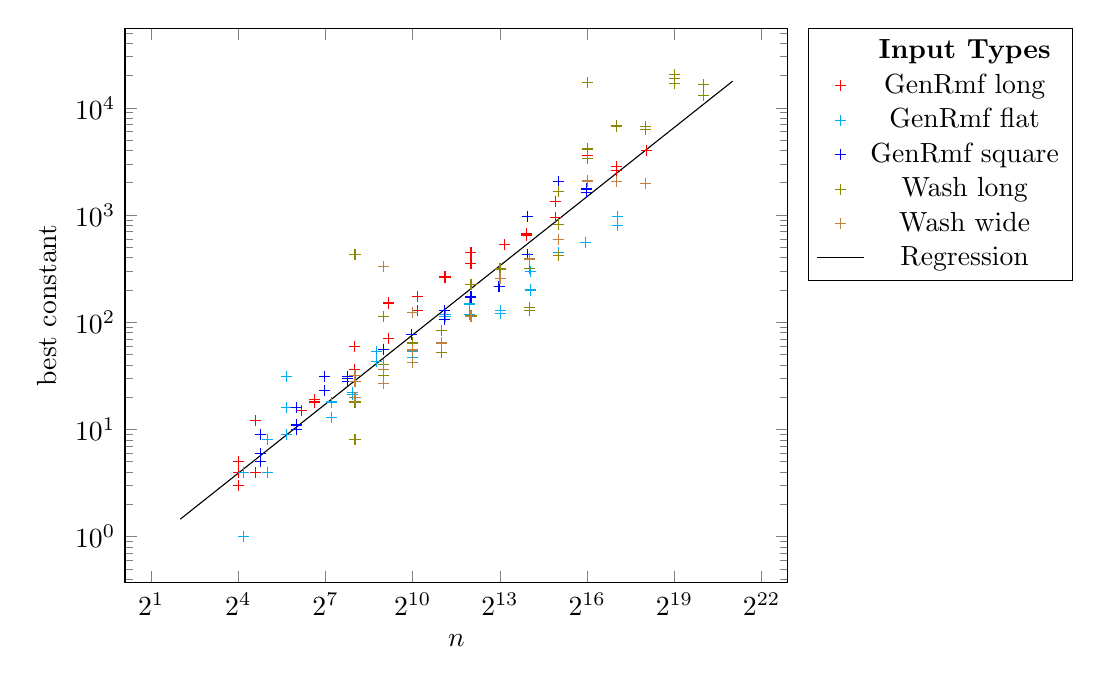
\begin{tikzpicture}
\begin{axis}[
    xlabel=$n$,ylabel=best constant,
    xmode=log,ymode=log,
    log basis x={2},
    legend style=
    {
        legend pos=outer north east
    },
    width=10cm
]
\addlegendimage{legend image code/.code=}
\legend{\textbf{Input Types}, GenRmf long, GenRmf flat, GenRmf square, Wash long, Wash wide, Regression}
\addplot [mark=+, red, only marks]table[x=n,y=value] {%GenRmf long
n   value
16	4
24	4
72	15
99	18
256	59
575	71
1152	175
2205	264
4096	352
9100	532
15488	650
30589	1327
65536	3584
130682	2582
270848	4020
16	5
24	4
72	15
99	18
256	36
575	151
1152	175
2205	264
4096	352
9100	532
15488	650
30589	1327
65536	3584
130682	2809
270848	4020
16	3
24	12
72	15
99	19
256	36
575	71
1152	129
2205	265
4096	448
9100	532
15488	665
30589	940
65536	3584
130682	2614
270848	3983
};
\addplot [mark=+, cyan, only marks]table[x=n,y=value] {%GenRmf flat
n   value
18	4
32	4
50	9
147	18
243	22
432	43
1024	53
2205	119
3920	148
8214	120
16807	200
32768	444
63504	558
135531	801
32	8
50	31
147	18
243	21
432	53
1024	47
2205	114
3920	118
8214	120
16807	196
32768	444
63504	558
135531	800
18	1
32	4
50	16
147	13
243	21
432	43
1024	53
2205	112
3920	118
8214	128
16807	296
32768	444
63504	558
135531	966
};
\addplot [mark=+, blue, only marks]table[x=n,y=value] {%GenRmf square
n   value
27	5
27	5
64	10
125	23
216	30
512	56
1000	77
2197	106
4096	172
8000	216
15625	427
32768	2040
64000	1624
27	5
27	5
64	16
125	23
216	31
512	56
1000	77
2197	128
4096	172
8000	216
15625	427
32768	2040
64000	1750
27	6
27	9
64	11
125	31
216	28
512	56
1000	77
2197	128
4096	172
8000	216
15625	976
32768	2048
64000	1750
};
\addplot [mark=+, olive, only marks]table[x=n,y=value] {%Wash long
n   value
258	429
514	40
1026	64
2050	52
4098	112
8194	318
16386	136
32770	812
65538	3344
131074	6648
262146	6752
524290	18656
1048578	16512
258	8
514	112
1026	64
2050	84
4098	116
8194	313
16386	128
32770	1664
65538	4128
131074	6880
262146	6656
524290	16704
1048578	12928
258	18
514	32
1026	64
2050	52
4098	223
8194	320
16386	320
32770	416
65538	17289
131074	6678
262146	6272
524290	20480
1048578	16384
};
\addplot [mark=+, brown, only marks]table[x=n,y=value] {%Wash wide
n   value
258	20
514	27
1026	124
2050	64
4098	112
8194	256
16386	392
32770	592
65538	2112
131074	2048
262146	1984
258	28
514	333
1026	42
2050	64
4098	112
8194	256
16386	384
32770	588
65538	2112
131074	2048
262146	1984
258	32
514	36
1026	55
2050	64
4098	113
8194	256
16386	384
32770	592
65538	2047
131074	2048
262146	1984
};
\addplot [domain=4:2097152]{0.54*x^0.7144};
\end{axis}
\end{tikzpicture}
\caption{Constant estimation for Global Relabel with node count trigger for Goldberg Tarjan Dynamic (GT D GRN)}
\label{fig:GT_D_GRN_Constant}
\end{figure}



\begin{figure}[h]
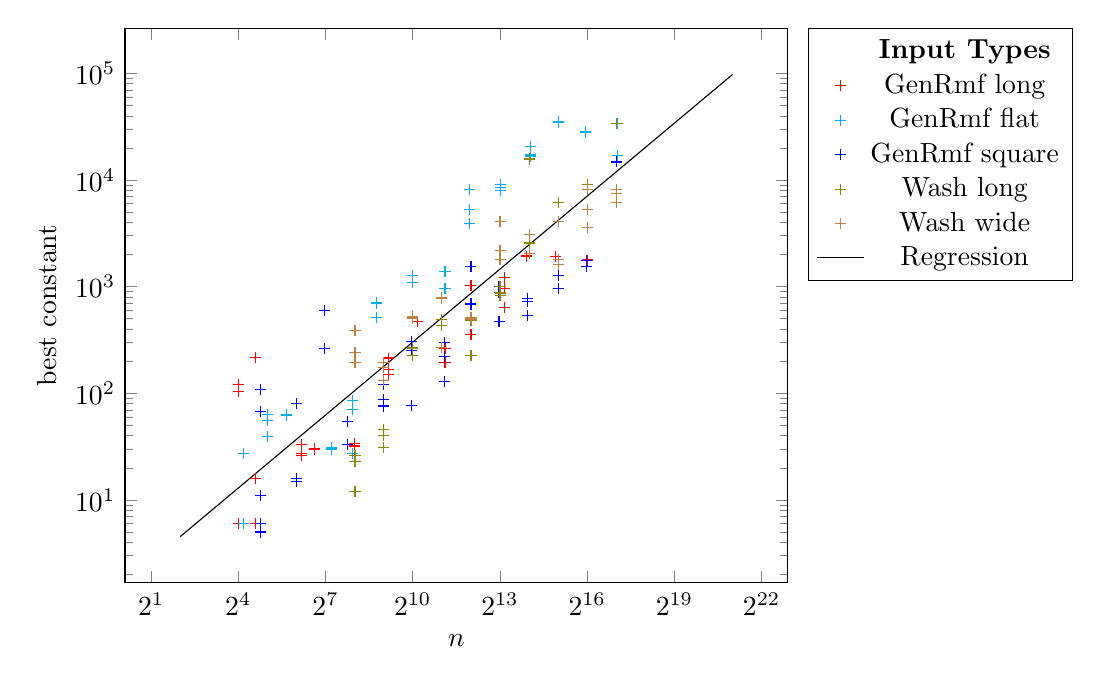
\begin{tikzpicture}
\begin{axis}[
    xlabel=$n$,ylabel=best constant,
    xmode=log,ymode=log,
    log basis x={2},
    legend style=
    {
        legend pos=outer north east
    },
    width=10cm
]
\addlegendimage{legend image code/.code=}
\legend{\textbf{Input Types}, GenRmf long, GenRmf flat, GenRmf square, Wash long, Wash wide, Regression}
\addplot [mark=+, red, only marks]table[x=n,y=value] {%GenRmf long
n   value
16	6
24	217
72	33
99	30
256	34
575	151
1152	468
2205	261
4096	1024
9100	643
15488	1928
30589	1911
65536	1776
16	121
24	16
72	27
99	30
256	32
575	214
1152	468
2205	261
4096	356
9100	960
15488	1928
30589	1911
65536	1776
16	104
24	6
72	26
99	30
256	32
575	167
1152	468
2205	196
4096	1024
9100	1208
15488	1936
30589	1911
65536	1776
};
\addplot [mark=+, cyan, only marks]table[x=n,y=value] {%GenRmf flat
n   value
18	6
32	39
50	62
147	30
243	86
432	702
1024	1092
2205	964
3920	5259
8214	8426
16807	20421
32768	34712
63504	28775
135531	16941
18	27
32	63
50	63
147	31
243	27
432	708
1024	1276
2205	1377
3920	3896
8214	9111
16807	16807
32768	35300
63504	27783
135531	33882	
32	56
50	62
147	30
243	71
432	509
1024	1276
2205	966
3920	8085
8214	7961
16807	17332
32768	35332
63504	28771
135531	16941
};
\addplot [mark=+, blue, only marks]table[x=n,y=value] {%GenRmf square
n   value
27	108
64	15	
216	33
512	88
1000	305
2197	299
4096	687
8000	875
15625	537
32768	960
64000	1765
132651	14768
27	6
27	11
64	80
125	265
216	54
512	76
1000	77
2197	222	
8000	468
15625	732
32768	952
64000	1531
132651	14767
27	5
27	67
64	16
125	598
216	33
512	120
1000	250
2197	128
4096	1552
8000	1000
15625	777
32768	1280
64000	1765
132651	14768
};
\addplot [mark=+, olive, only marks]table[x=n,y=value] {%Wash long
n   value
258	23
514	40
1026	228
2050	495
4098	483
8194	871
16386	2560
32770	6209
65538	9092
131074	33792
258	26
514	31
1026	228
2050	432
4098	224
8194	832
16386	2584
32770	6209
65538	9094
131074	33792
258	12
514	46
1026	266
2050	433
4098	482
8194	1006
16386	15753
32770	6172
65538	9094
131074	33728
};
\addplot [mark=+, brown, only marks]table[x=n,y=value] {%Wash wide
n   value
258	240
514	174
1026	513
2050	787
4098	498
8194	1797
16386	3080
32770	1600
65538	5248
131074	8160
258	385
514	132
1026	500
2050	270
4098	496
8194	4075
16386	2048
32770	1792
65538	8192
131074	7480
258	196
514	196
1026	522
2050	767
4098	512
8194	2179
16386	2054
32770	4066
65538	3584
131074	6147
};
\addplot [domain=4:2097152]{1.5834*x^0.7578};
\end{axis}
\end{tikzpicture}
\caption{Constant estimation for Global Relabel with node count trigger for King Rao Low Memory (GT LM GRN)}
\label{fig:KR LM_GRN_Constant}
\end{figure}



\begin{figure}[h]
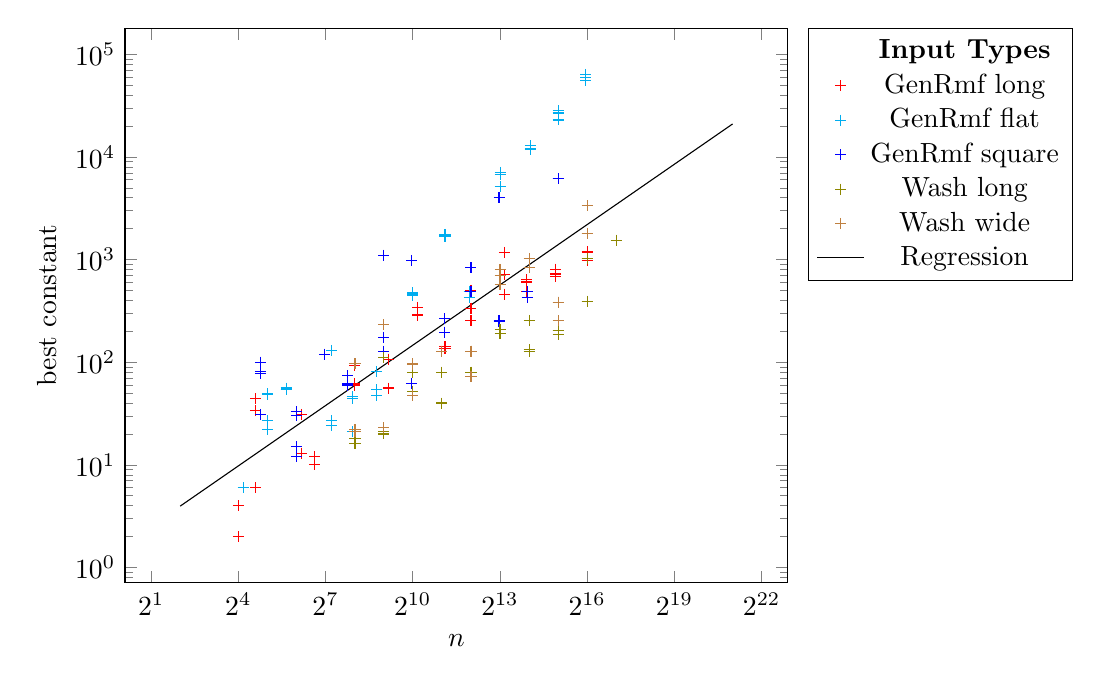
\begin{tikzpicture}
\begin{axis}[
    xlabel=$n$,ylabel=best constant,
    xmode=log,ymode=log,
    log basis x={2},
    legend style=
    {
        legend pos=outer north east
    },
    width=10cm
]
\addlegendimage{legend image code/.code=}
\legend{\textbf{Input Types}, GenRmf long, GenRmf flat, GenRmf square, Wash long, Wash wide, Regression}
\addplot [mark=+, red, only marks]table[x=n,y=value] {%GenRmf long
n   value
24	44
72	13
99	10
256	92
575	107
1152	288
2205	141
4096	336
9100	1172
15488	635
30589	804
65536	1184
16	4
24	34
72	13
99	12
256	60
575	107
1152	342
2205	141
4096	254
9100	711
15488	605
30589	681
65536	1029
16	2
24	6
72	31
99	10
256	62
575	56
1152	290
2205	137
4096	501
9100	461
15488	484
30589	723
65536	972
};
\addplot [mark=+, cyan, only marks]table[x=n,y=value] {%GenRmf flat
n   value
18	6
32	27
50	54
147	27
243	44
432	47
1024	456
2205	1756
3920	490
8214	5133
16807	11782
32768	26752
63504	55806
18	6
32	22
50	54
147	24
243	46
432	81
1024	448
2205	1684
3920	490
8214	7056
16807	12079
32768	28288
63504	59535
18	6
32	49
50	56
147	130
243	21
432	54
1024	472
2205	1703
3920	426
8214	6673
16807	12876
32768	22896
63504	63566
};
\addplot [mark=+, blue, only marks]table[x=n,y=value] {%GenRmf square
n   value
27	81
64	15	
216	74
512	175
1000	62
2197	196
4096	832
8000	255
15625	488
32768	6144	
27	77
64	12	
216	60
512	128
1000	62
2197	196
4096	832
8000	250
15625	431
32768	6144	
27	100
64	30
27	31
64	33
125	120
216	62
512	1102
1000	979
2197	265
4096	488
8000	4032
};
\addplot [mark=+, olive, only marks]table[x=n,y=value] {%Wash long
n   value
258	18
514	20
1026	52
2050	80
4098	80
8194	207
16386	132
32770	204
65538	392
131074	1536
258	16
514	21
1026	52
2050	40
4098	73
8194	191
16386	256
32770	204
65538	392
131074	1540	
514	111
1026	80	
4098	73	
16386	128
32770	188
65538	1024
131074	1536
};
\addplot [mark=+, brown, only marks]table[x=n,y=value] {%Wash wide
n   value
258	22
514	23
1026	96
2050	128
4098	73
8194	800
16386	1016
32770	384
65538	1796
258	21
514	23
1026	96
2050	128
4098	128
8194	577
16386	836
32770	384
65538	1792
258	97
514	232
1026	47
2050	128
4098	128
8194	704
16386	832
32770	254
65538	3336
};
\addplot [domain=4:2097152]{1.6078*x^0.6509};
\end{axis}
\end{tikzpicture}
\caption{Constant estimation for Global Relabel with node count trigger for King Rao Low Memory Dynamic (KR LM D GRN)}
\label{fig:KR_LM_GRN_Constant}
\end{figure}

    
\clearpage
\section{Charts}
\label{ChartAppendix}


\subsection{Results from CRH graphs}
\begin{figure}[h]
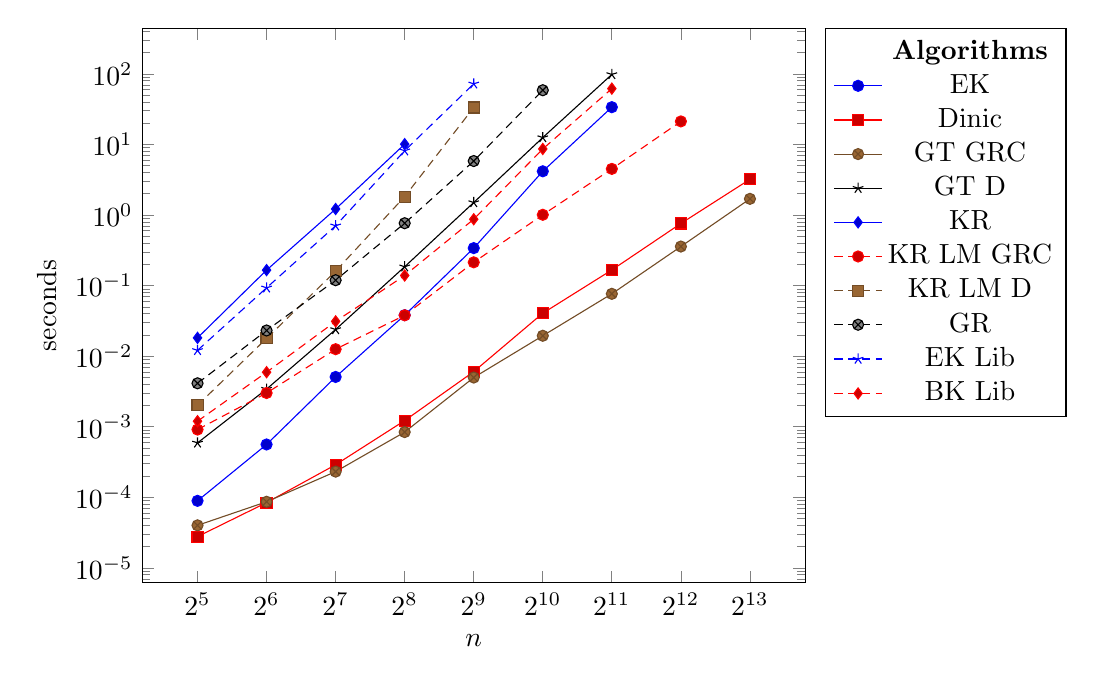
\begin{tikzpicture}
\begin{axis}[
    xlabel=$n$,ylabel=seconds,
    xmode=log,ymode=log,
    log basis x={2},
    legend style=
    {
        legend pos=outer north east
    },
    width=10cm
]
\addlegendimage{legend image code/.code=}
\legend{\textbf{Algorithms}, EK, Dinic, GT GRC, GT D, KR, KR LM GRC, KR LM D, GR, EK Lib, BK Lib}
\addplot table[x=n,y=value] {%EK
n value
32	8.91727E-05
64	0.00056091
128	0.005077953
256	0.038123333
512	0.339550667
1024	4.16451
2048	33.72456667
};
\addplot table[x=n,y=value] {%Dinic
n value
32	2.77623E-05
64	8.41754E-05
128	0.000289727
256	0.001222433
512	0.006034197
1024	0.040603633
2048	0.166434667
4096	0.758745667
8192	3.204413333
};
\addplot table[x=n,y=value] {%GT GRC
n value
32	4.00888E-05
64	8.65074E-05
128	0.000231315
256	0.000840643
512	0.004980787
1024	0.019460933
2048	0.0764499
4096	0.357635
8192	1.694086667
};
\addplot table[x=n,y=value] {%GT D
n value
32	0.000590562
64	0.003415777
128	0.023887433
256	0.185035333
512	1.504396667
1024	12.51486667
2048	98.09486667
};
\addplot table[x=n,y=value] {%KR
n value
32	0.0181733
64	0.165739667
128	1.21656
256	10.09223333
};
\addplot table[x=n,y=value] {%KR LM GRC
n value
32	0.000912274
64	0.00300656
128	0.012558933
256	0.037942
512	0.213656667
1024	1.007368333
2048	4.502716667
4096	21.199
};
\addplot table[x=n,y=value] {%KR LM D
n value
32	0.002014107
64	0.017856
128	0.16025
256	1.82407
512	33.37643333
};
\addplot table[x=n,y=value] {%GR
n value
32	0.004126927
64	0.023131233
128	0.119142333
256	0.765221333
512	5.817686667
1024	58.60563333
};
\addplot table[x=n,y=value] {%EK Lib
n value
32	0.0120941
64	0.092989167
128	0.704491333
256	8.1467
512	72.2544
};
\addplot table[x=n,y=value] {%BK Lib
n value
32	0.001199007
64	0.00592652
128	0.031122567
256	0.138813
512	0.871689667
1024	8.632126667
2048	61.7279
};
\end{axis}
\end{tikzpicture}
\caption{Best and worst results from the CRH graphs}
\label{fig:CRH_BW_Results}
\end{figure}


\begin{figure}[h]
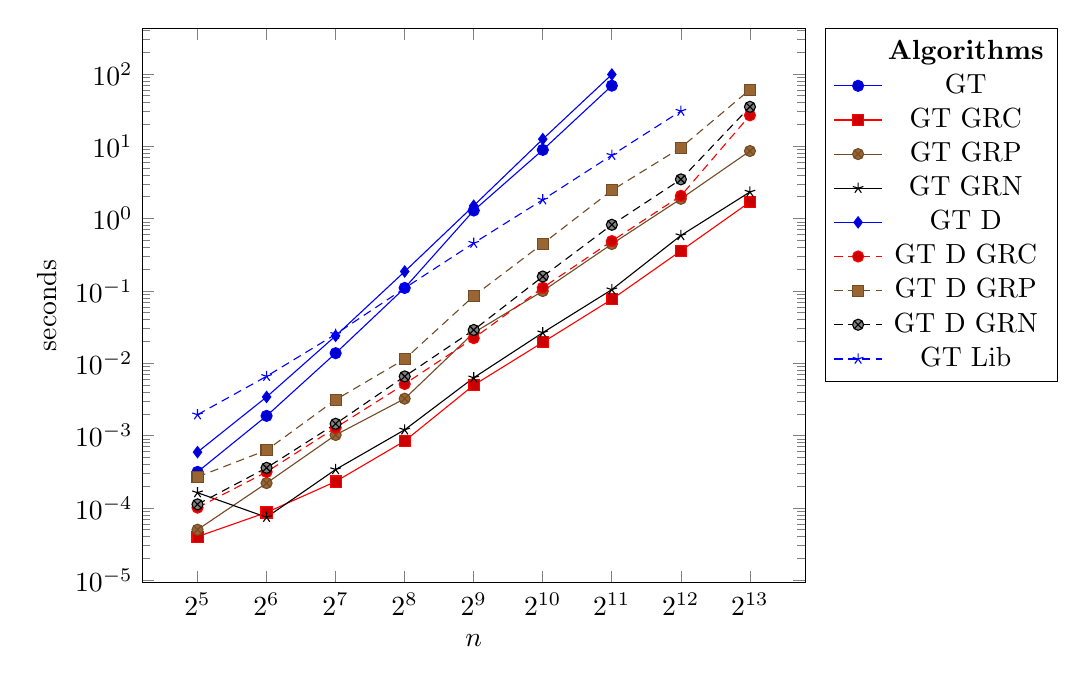
\begin{tikzpicture}
\begin{axis}[
    xlabel=$n$,ylabel=seconds,
    xmode=log,ymode=log,
    log basis x={2},
    legend style=
    {
        legend pos=outer north east
    },
    width=10cm
]
\addlegendimage{legend image code/.code=}
\legend{\textbf{Algorithms}, GT, GT GRC, GT GRP, GT GRN, GT D, GT D GRC, GT D GRP, GT D GRN, GT Lib}
\addplot table[x=n,y=value] {%GT
n value
32	0.000314492
64	0.001870183
128	0.0137617
256	0.109700333
512	1.290522
1024	8.888233333
2048	68.60676667
};
\addplot table[x=n,y=value] {%GT GRC
n value
32	4.00888E-05
64	8.65074E-05
128	0.000231315
256	0.000840643
512	0.004980787
1024	0.019460933
2048	0.0764499
4096	0.357635
8192	1.694086667
};
\addplot table[x=n,y=value] {%GT GRP
n value
32	4.99722E-05
64	0.000220322
128	0.0010181
256	0.003234533
512	0.026379533
1024	0.0994381
2048	0.444045
4096	1.873073333
8192	8.57279
};
\addplot table[x=n,y=value] {%GT GRN
n value
32	0.000162244
64	7.41812E-05
128	0.000339257
256	0.00120067
512	0.00629929
1024	0.0264405
2048	0.104068667
4096	0.582426667
8192	2.32921
};
\addplot table[x=n,y=value] {%GT D
n value
32	0.000590562
64	0.003415777
128	0.023887433
256	0.185035333
512	1.504396667
1024	12.51486667
2048	98.09486667
};
\addplot table[x=n,y=value] {%GT D GRC
n value
32	0.000100833
64	0.000313938
128	0.001286068
256	0.005157717
512	0.022182613
1024	0.1106239
2048	0.488021
4096	2.059113333
8192	26.67935333
};
\addplot table[x=n,y=value] {%GT D GRP
n value
32	0.000268296
64	0.000627764
128	0.003125717
256	0.011373383
512	0.084937633
1024	0.449372
2048	2.45048
4096	9.537386667
8192	60.5804
};
\addplot table[x=n,y=value] {%GT D GRN
n value
32	0.000111938
64	0.000358024
128	0.001454862
256	0.006570687
512	0.028821933
1024	0.157848667
2048	0.818823
4096	3.477246667
8192	34.995
};
\addplot table[x=n,y=value] {%GT Lib
n value
32	0.00194182
64	0.00659182
128	0.025150267
256	0.109139667
512	0.457306667
1024	1.818046667
2048	7.501273333
4096	30.58266667
};
\end{axis}
\end{tikzpicture}
\caption{Goldberg and Tarjan results from the CRH graphs}
\label{fig:CRH_GT_Results}
\end{figure}


\begin{figure}[h]
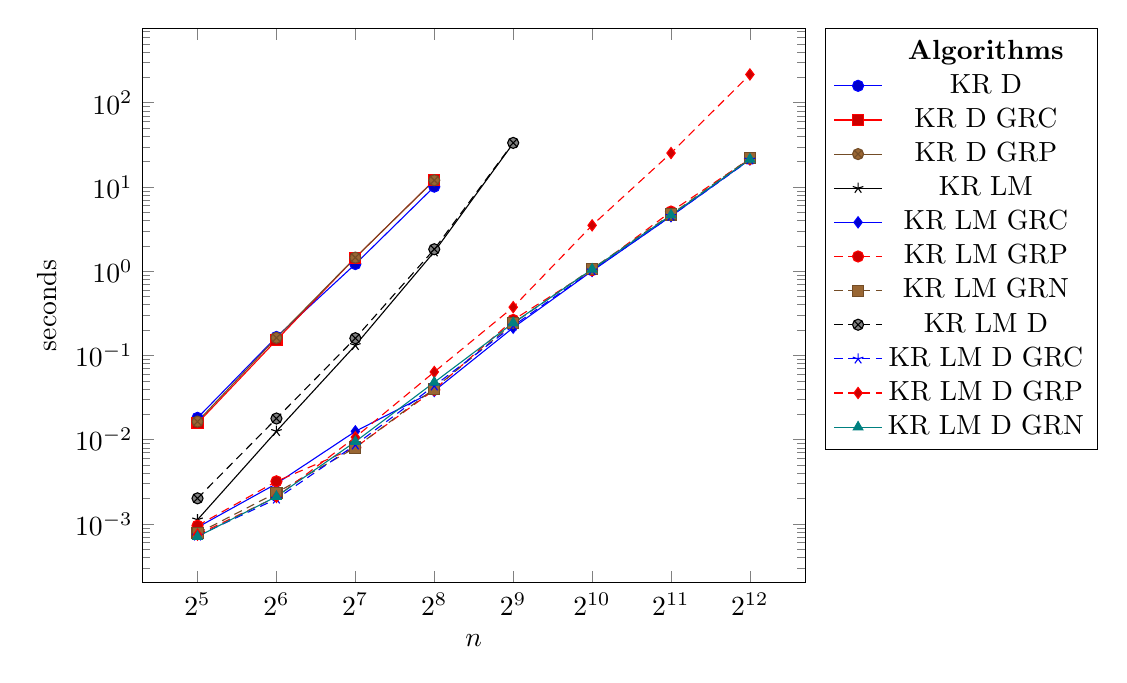
\begin{tikzpicture}
\begin{axis}[
    xlabel=$n$,ylabel=seconds,
    xmode=log,ymode=log,
    log basis x={2},
    legend style=
    {
        legend pos=outer north east
    },
    width=10cm
]
\addlegendimage{legend image code/.code=}
\legend{\textbf{Algorithms}, KR D, KR D GRC, KR D GRP, KR LM, KR LM GRC, KR LM GRP, KR LM GRN, KR LM D, KR LM D GRC, KR LM D GRP, KR LM D GRN}
\addplot table[x=n,y=value] {%KR
n value
32	0.0181733
64	0.165739667
128	1.21656
256	10.09223333
};
\addplot table[x=n,y=value] {%KR GRC
n value
32	0.0156879
64	0.151962
128	1.45053
256	12.0393
};
\addplot table[x=n,y=value] {%KR GRP
n value
32	0.016405833
64	0.162039667
128	1.45158
256	12.01736667
};
\addplot table[x=n,y=value] {%KR LM
n value
32	0.00112349
64	0.012595033
128	0.131954333
256	1.705006667
512	32.9077
};
\addplot table[x=n,y=value] {%KR LM GRC
n value
32	0.000912274
64	0.00300656
128	0.012558933
256	0.037942
512	0.213656667
1024	1.007368333
2048	4.502716667
4096	21.199
};
\addplot table[x=n,y=value] {%KR LM GRP
n value
32	0.00095436
64	0.003208227
128	0.00807021
256	0.0391309
512	0.264306667
1024	1.029762667
2048	5.10844
4096	21.54473333
};
\addplot table[x=n,y=value] {%KR LM GRN
n value
32	0.000772573
64	0.002344813
128	0.008068313
256	0.040385667
512	0.240289667
1024	1.069216667
2048	4.716753333
4096	21.92293333
};
\addplot table[x=n,y=value] {%KR LM D
n value
32	0.002014107
64	0.017856
128	0.16025
256	1.82407
512	33.37643333
};
\addplot table[x=n,y=value] {%KR LM D GRC
n value
32	0.000722157
64	0.001982017
128	0.00869863
256	0.043668633
512	0.224592667
1024	1.017951333
2048	4.51069
4096	21.01986667
};
\addplot table[x=n,y=value] {%KR LM D GRP
n value
32	0.000746587
64	0.002094287
128	0.010713517
256	0.063737267
512	0.374642667
1024	3.505513333
2048	25.29676667
4096	216.746
};
\addplot[mark=triangle*, teal] table[x=n,y=value] {%KR LM D GRN
n value
32	0.000707387
64	0.002113277
128	0.009478093
256	0.0480019
512	0.243291
1024	1.052536667
2048	4.632166667
4096	21.3589
};
\end{axis}
\end{tikzpicture}
\caption{King and Rao results from the CRH graphs}
\label{fig:CRH_KR_Results}
\end{figure}

%-----------------------------------------------------------------------------------------------------------
\clearpage


\subsection{Results from CRE graphs}
\begin{figure}[h]
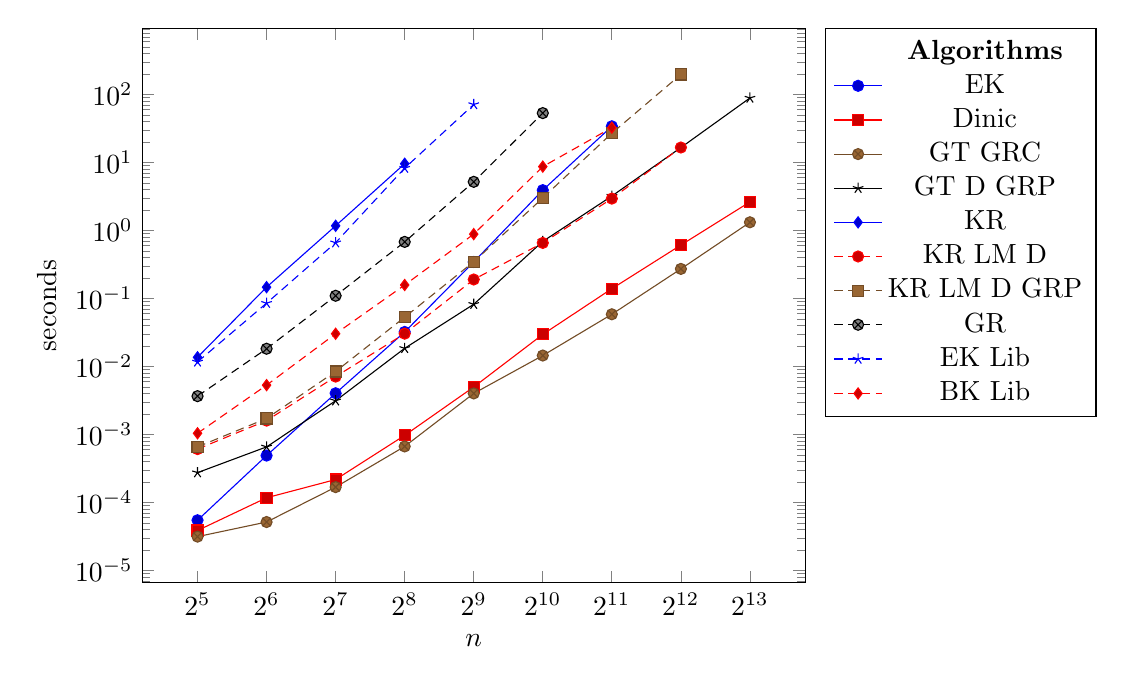
\begin{tikzpicture}
\begin{axis}[
    xlabel=$n$,ylabel=seconds,
    xmode=log,ymode=log,
    log basis x={2},
    legend style=
    {
        legend pos=outer north east
    },
    width=10cm
]
\addlegendimage{legend image code/.code=}
\legend{\textbf{Algorithms}, EK, Dinic, GT GRC, GT D GRP, KR, KR LM D, KR LM D GRP, GR, EK Lib, BK Lib}
\addplot table[x=n,y=value] {%EK
n value
32	5.47473E-05
64	0.000488839
128	0.00403531
256	0.032188067
512	0.344482667
1024	3.92213
2048	34.09136667
};
\addplot table[x=n,y=value] {%Dinic
n value
32	3.86452E-05
64	0.000117157
128	0.000217213
256	0.000969461
512	0.004991113
1024	0.0296234
2048	0.13921
4096	0.610286667
8192	2.630443333
};
\addplot table[x=n,y=value] {%GT GRC
n value
32	3.1427E-05
64	5.15269E-05
128	0.000168017
256	0.000666518
512	0.00401199
1024	0.0144843
2048	0.0585542
4096	0.272228333
8192	1.320586667
};
\addplot table[x=n,y=value] {%GT D GRP
n value
32	0.000274404
64	0.000656526
128	0.003130713
256	0.018493567
512	0.082231433
1024	0.691143667
2048	3.20825
4096	16.5731
8192	88.89143333
};
\addplot table[x=n,y=value] {%KR
n value
32	0.013644
64	0.146774
128	1.172116667
256	9.59715
};
\addplot table[x=n,y=value] {%KR LM D
n value
32	0.000609217
64	0.00159878
128	0.007093297
256	0.030375067
512	0.190262667
1024	0.656387333
2048	2.943613333
4096	16.61786667
};
\addplot table[x=n,y=value] {%KR LM D GRP
n value
32	0.000656525
64	0.001718273
128	0.008436667
256	0.0530621
512	0.346809
1024	3.012093333
2048	26.94046667
4096	197.305
};
\addplot table[x=n,y=value] {%GR
n value
32	0.003658853
64	0.0182312
128	0.109624667
256	0.679776333
512	5.196073333
1024	53.29516667
};
\addplot table[x=n,y=value] {%EK Lib
n value
32	0.011662833
64	0.0852518
128	0.661307667
256	8.265413333
512	71.3308
};
\addplot table[x=n,y=value] {%BK Lib
n value
32	0.001040203
64	0.005313077
128	0.030276133
256	0.157713
512	0.884518333
1024	8.698513333
2048	32.59023333
};
\end{axis}
\end{tikzpicture}
\caption{Best and worst results from the CRE graphs}
\label{fig:CRE_BW_Results}
\end{figure}


\begin{figure}[h]
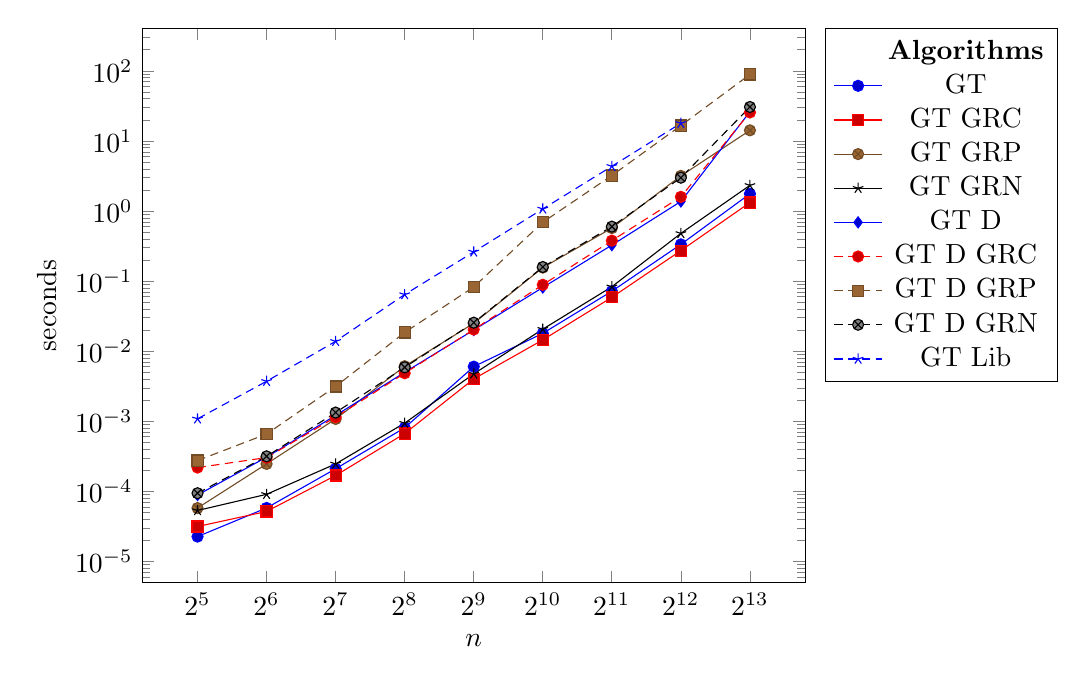
\begin{tikzpicture}
\begin{axis}[
    xlabel=$n$,ylabel=seconds,
    xmode=log,ymode=log,
    log basis x={2},
    legend style=
    {
        legend pos=outer north east
    },
    width=10cm
]
\addlegendimage{legend image code/.code=}
\legend{\textbf{Algorithms}, GT, GT GRC, GT GRP, GT GRN, GT D, GT D GRC, GT D GRP, GT D GRN, GT Lib}
\addplot table[x=n,y=value] {%GT
n value
32	0.000022543
64	5.78567E-05
128	0.000209439
256	0.000805885
512	0.006011103
1024	0.017948133
2048	0.071653367
4096	0.334158333
8192	1.76081
};
\addplot table[x=n,y=value] {%GT GRC
n value
32	3.1427E-05
64	5.15269E-05
128	0.000168017
256	0.000666518
512	0.00401199
1024	0.0144843
2048	0.0585542
4096	0.272228333
8192	1.320586667
};
\addplot table[x=n,y=value] {%GT GRP
n value
32	5.76346E-05
64	0.000245974
128	0.001076403
256	0.006092387
512	0.025003667
1024	0.155701
2048	0.570373667
4096	3.17186
8192	14.16263333
};
\addplot table[x=n,y=value] {%GT GRN
n value
32	5.31928E-05
64	9.05055E-05
128	0.000245975
256	0.000939036
512	0.004738823
1024	0.0205873
2048	0.082965767
4096	0.479294
8192	2.32381
};
\addplot table[x=n,y=value] {%GT D
n value
32	8.83956E-05
64	0.000307163
128	0.001209329
256	0.004990683
512	0.020028707
1024	0.081005167
2048	0.326051
4096	1.369142
8192	26.16655333
};
\addplot table[x=n,y=value] {%GT D GRC
n value
32	0.00021788
64	0.000302722
128	0.001143924
256	0.00483831
512	0.02032443
1024	0.088531933
2048	0.378064333
4096	1.592337667
8192	25.48298667
};
\addplot table[x=n,y=value] {%GT D GRP
n value
32	0.000274404
64	0.000656526
128	0.003130713
256	0.018493567
512	0.082231433
1024	0.691143667
2048	3.20825
4096	16.5731
8192	88.89143333
};
\addplot table[x=n,y=value] {%GT D GRN
n value
32	9.38368E-05
64	0.000315492
128	0.001328933
256	0.005874867
512	0.0254909
1024	0.158821667
2048	0.598509
4096	2.988956667
8192	30.53813333
};
\addplot table[x=n,y=value] {%GT Lib
n value
32	0.00108196
64	0.003715623
128	0.013819433
256	0.064229333
512	0.260638667
1024	1.070513333
2048	4.344643333
4096	17.865
};
\end{axis}
\end{tikzpicture}
\caption{Goldberg and Tarjan results from the CRE graphs}
\label{fig:CRE_GT_Results}
\end{figure}


\begin{figure}[h]
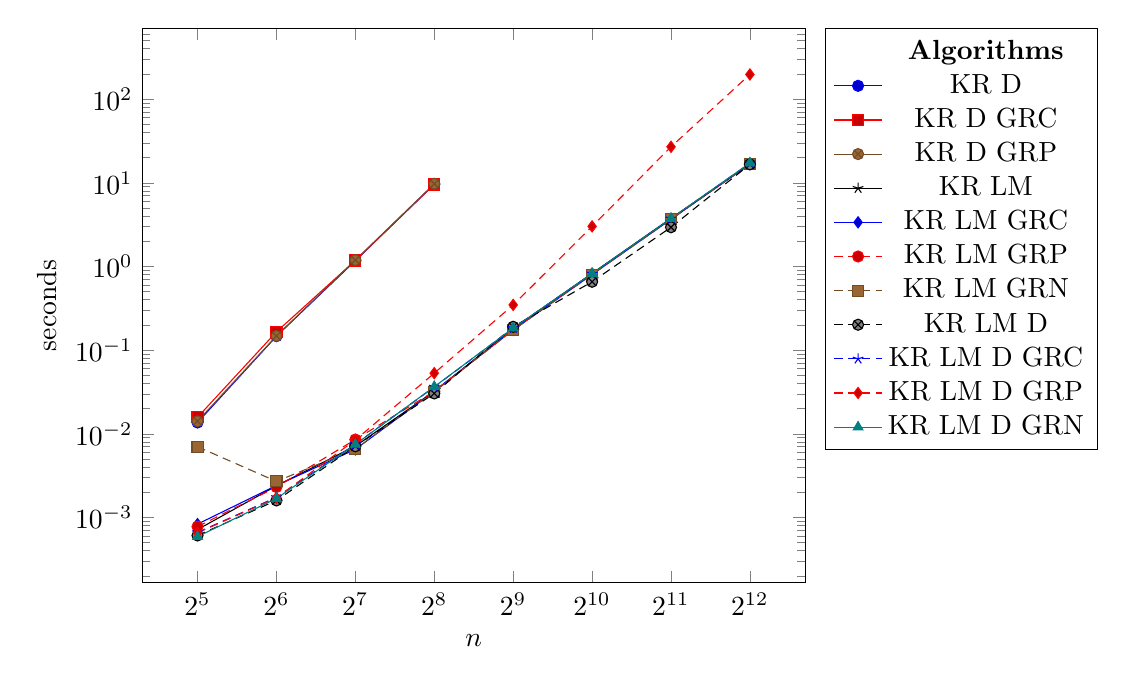
\begin{tikzpicture}
\begin{axis}[
    xlabel=$n$,ylabel=seconds,
    xmode=log,ymode=log,
    log basis x={2},
    legend style=
    {
        legend pos=outer north east
    },
    width=10cm
]
\addlegendimage{legend image code/.code=}
\legend{\textbf{Algorithms}, KR D, KR D GRC, KR D GRP, KR LM, KR LM GRC, KR LM GRP, KR LM GRN, KR LM D, KR LM D GRC, KR LM D GRP, KR LM D GRN}
\addplot table[x=n,y=value] {%KR
n value
32	0.013644
64	0.146774
128	1.172116667
256	9.59715
};
\addplot table[x=n,y=value] {%KR GRC
n value
32	0.015749367
64	0.165407333
128	1.180593333
256	9.566476667
};
\addplot table[x=n,y=value] {%KR GRP
n value
32	0.014125267
64	0.147867
128	1.192166667
256	9.735496667
};
\addplot table[x=n,y=value] {%KR LM
n value
32	0.000716493
64	0.002392677
128	0.007121063
256	0.0321503
512	0.180944667
1024	0.826992
2048	3.762636667
4096	16.7083
};
\addplot table[x=n,y=value] {%KR LM GRC
n value
32	0.00083254
64	0.002410663
128	0.006525943
256	0.032414067
512	0.174600667
1024	0.801770333
2048	3.67155
4096	16.72523333
};
\addplot table[x=n,y=value] {%KR LM GRP
n value
32	0.000777125
64	0.0023105
128	0.008542273
256	0.0321469
512	0.175911
1024	0.808778333
2048	3.688806667
4096	16.86536667
};
\addplot table[x=n,y=value] {%KR LM GRN
n value
32	0.007005796
64	0.002697727
128	0.006570027
256	0.031863467
512	0.173352333
1024	0.798951667
2048	3.65546
4096	16.72086667
};
\addplot table[x=n,y=value] {%KR LM D
n value
32	0.000609217
64	0.00159878
128	0.007093297
256	0.030375067
512	0.190262667
1024	0.656387333
2048	2.943613333
4096	16.61786667
};
\addplot table[x=n,y=value] {%KR LM D GRC
n value
32	0.00066219
64	0.001740923
128	0.007506513
256	0.0362996
512	0.183215667
1024	0.817935
2048	3.727963333
4096	17.15916667
};
\addplot table[x=n,y=value] {%KR LM D GRP
n value
32	0.000656525
64	0.001718273
128	0.008436667
256	0.0530621
512	0.346809
1024	3.012093333
2048	26.94046667
4096	197.305
};
\addplot[mark=triangle*, teal] table[x=n,y=value] {%KR LM D GRN
n value
32	0.000590452
64	0.00168551
128	0.00747431
256	0.036542667
512	0.183141
1024	0.823798
2048	3.743673333
4096	17.22786667
};
\end{axis}
\end{tikzpicture}
\caption{King and Rao results from the CRE graphs}
\label{fig:CRE_KR_Results}
\end{figure}

%-----------------------------------------------------------------------------------------------------------

\clearpage

\subsection{Results from CD graphs}
\begin{figure}[h]
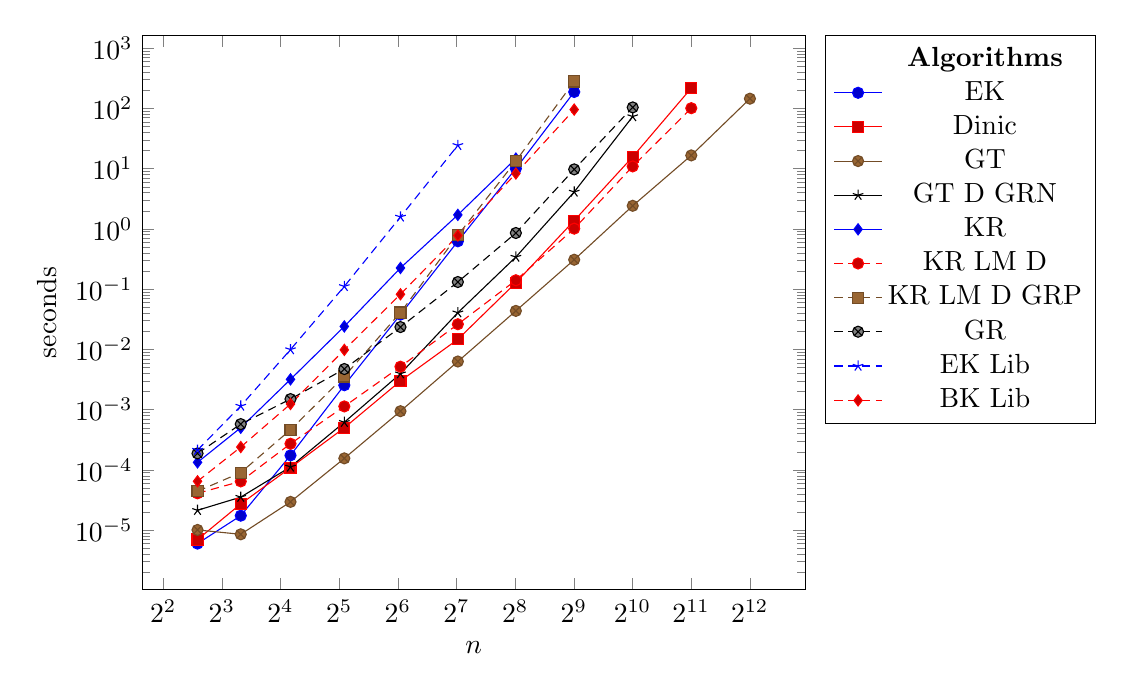
\begin{tikzpicture}
\begin{axis}[
    xlabel=$n$,ylabel=seconds,
    xmode=log,ymode=log,
    log basis x={2},
    legend style=
    {
        legend pos=outer north east
    },
    width=10cm
]
\addlegendimage{legend image code/.code=}
\legend{\textbf{Algorithms}, EK, Dinic, GT, GT D GRN, KR, KR LM D, KR LM D GRP, GR, EK Lib, BK Lib}
\addplot table[x=n,y=value] {%EK
n value
6	5.99667E-06
10	1.74347E-05
18	0.000174792
34	0.002550027
66	0.037885933
130	0.624042667
258	10.04213333
514	187.6203333
};
\addplot table[x=n,y=value] {%Dinic
n value
6	6.99611E-06
10	2.73181E-05
18	0.00010905
34	0.000501499
66	0.00300133
130	0.0147208
258	0.128177333
514	1.37476
1026	15.72296667
2050	217.4116667
};
\addplot table[x=n,y=value] {%GT
n value
6	1.01055E-05
10	8.5508E-06
18	2.95391E-05
34	0.000155802
66	0.000944475
130	0.006306823
258	0.043635633
514	0.308285667
1026	2.421146667
2050	16.61676667
4098	145.0676667
};
\addplot table[x=n,y=value] {%GT D GRN
n value
6	2.14326E-05
10	3.54248E-05
18	0.000112493
34	0.00061999
66	0.003963697
130	0.040730567
258	0.341904333
514	4.108336667
1026	73.36176667
};
\addplot table[x=n,y=value] {%KR
n value
6	0.000133704
10	0.000502276
18	0.00318767
34	0.0240945
66	0.225141333
130	1.711946667
258	14.71456667
};
\addplot table[x=n,y=value] {%KR LM D
n value
6	4.09773E-05
10	6.46309E-05
18	0.000272405
34	0.00113404
66	0.00517125
130	0.0262096
258	0.140639
514	1.011333333
1026	10.91203333
2050	100.9013333
};
\addplot table[x=n,y=value] {%KR LM D GRP
n value
6	4.43088E-05
10	9.02832E-05
18	0.000464965
34	0.003558917
66	0.040930333
130	0.784254333
258	13.388
514	280.4783333
};
\addplot table[x=n,y=value] {%GR
n value
6	0.000188451
10	0.000577012
18	0.001500943
34	0.004733923
66	0.023517667
130	0.131538667
258	0.856225667
514	9.73903
1026	103.9606667
};
\addplot table[x=n,y=value] {%EK Lib
n value
6	0.000213883
10	0.00115181
18	0.009964183
34	0.111426
66	1.58397
130	24.43106667
};
\addplot table[x=n,y=value] {%BK Lib
n value
6	6.48532E-05
10	0.000239979
18	0.001242873
34	0.00983991
66	0.082395133
130	0.777942
258	8.31923
514	95.6544
};
\end{axis}
\end{tikzpicture}
\caption{Best and worst results from the CD graphs}
\label{fig:CD_BW_Results}
\end{figure}


\begin{figure}[h]
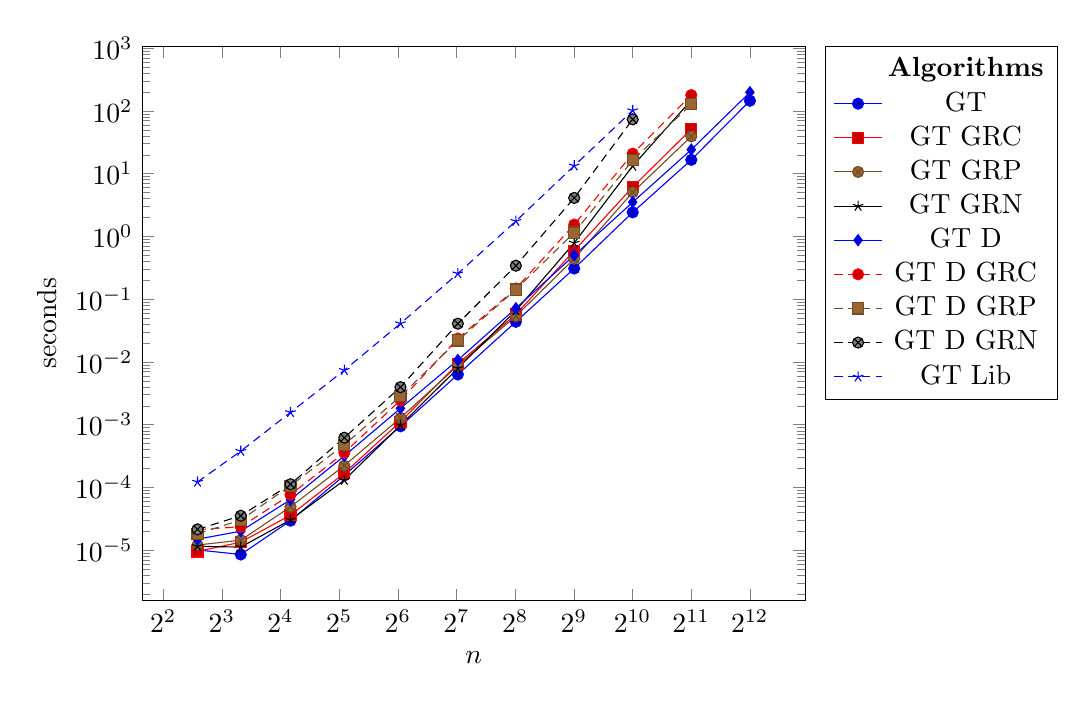
\begin{tikzpicture}
\begin{axis}[
    xlabel=$n$,ylabel=seconds,
    xmode=log,ymode=log,
    log basis x={2},
    legend style=
    {
        legend pos=outer north east
    },
    width=10cm
]
\addlegendimage{legend image code/.code=}
\legend{\textbf{Algorithms}, GT, GT GRC, GT GRP, GT GRN, GT D, GT D GRC, GT D GRP, GT D GRN, GT Lib}
\addplot table[x=n,y=value] {%GT
n value
6	1.01055E-05
10	8.5508E-06
18	2.95391E-05
34	0.000155802
66	0.000944475
130	0.006306823
258	0.043635633
514	0.308285667
1026	2.421146667
2050	16.61676667
4098	145.0676667
};
\addplot table[x=n,y=value] {%GT GRC
n value
6	9.55024E-06
10	1.34369E-05
18	3.62021E-05
34	0.000169017
66	0.001118267
130	0.009349797
258	0.057142333
514	0.591681667
1026	6.116086667
2050	51.259
};
\addplot table[x=n,y=value] {%GT GRP
n value
6	1.21044E-05
10	1.44364E-05
18	4.91949E-05
34	0.000222876
66	0.00128251
130	0.008756907
258	0.053604167
514	0.441572333
1026	5.047726667
2050	39.2892
};
\addplot table[x=n,y=value] {%GT GRN
n value
6	1.15492E-05
10	1.1216E-05
18	3.04276E-05
34	0.000130594
66	0.000979679
130	0.007932053
258	0.0657545
514	0.788411667
1026	13.26623333
2050	148.4456667
};
\addplot table[x=n,y=value] {%GT D
n value
6	1.49917E-05
10	2.01E-05
18	6.38536E-05
34	0.000318379
66	0.00181977
130	0.010725967
258	0.071542
514	0.499891
1026	3.513503333
2050	24.14273333
4098	198.0083333
};
\addplot table[x=n,y=value] {%GT D GRC
n value
6	2.13216E-05
10	2.36536E-05
18	7.66243E-05
34	0.000357802
66	0.00245109
130	0.023582033
258	0.147942
514	1.545093333
1026	20.85666667
2050	178.8586667
};
\addplot table[x=n,y=value] {%GT D GRP
n value
6	1.82122E-05
10	3.03165E-05
18	0.000106608
34	0.000480068
66	0.002840317
130	0.021989267
258	0.142533333
514	1.151853333
1026	16.32986667
2050	127.8266667
};
\addplot table[x=n,y=value] {%GT D GRN
n value
6	2.14326E-05
10	3.54248E-05
18	0.000112493
34	0.00061999
66	0.003963697
130	0.040730567
258	0.341904333
514	4.108336667
1026	73.36176667
};
\addplot table[x=n,y=value] {%GT Lib
n value
6	0.000122266
10	0.000379236
18	0.001570913
34	0.007375277
66	0.040921467
130	0.25571
258	1.75135
514	13.36043333
1026	101.6196667
};
\end{axis}
\end{tikzpicture}
\caption{Goldberg and Tarjan results from the CD graphs}
\label{fig:CD_GT_Results}
\end{figure}


\begin{figure}[h]
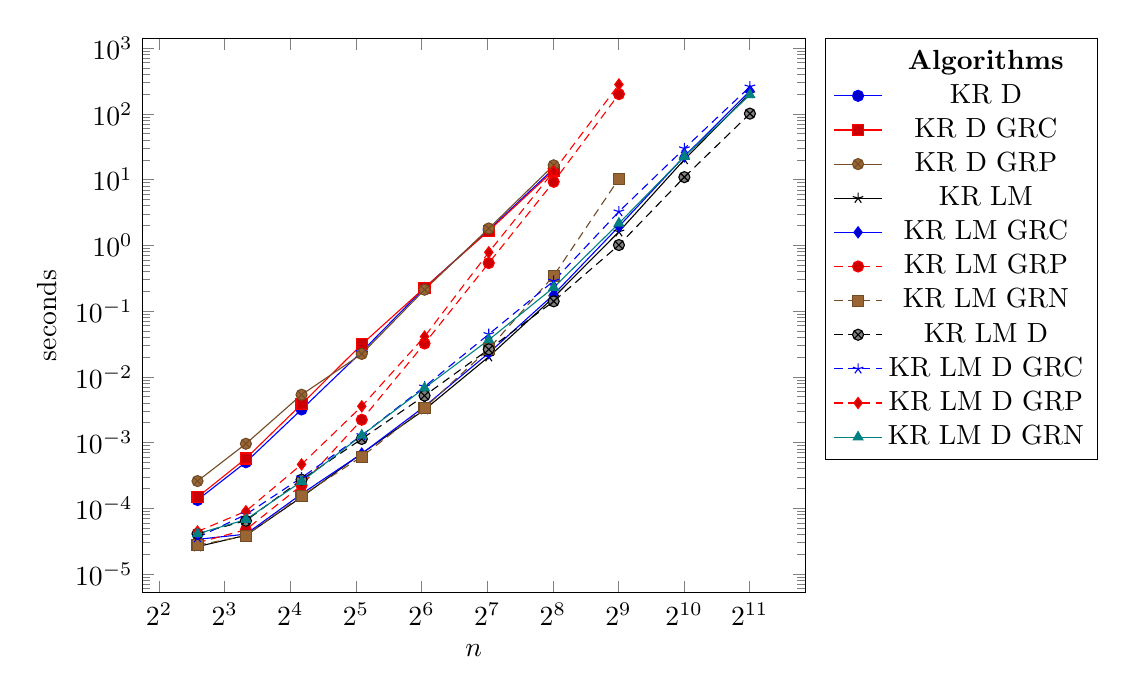
\begin{tikzpicture}
\begin{axis}[
    xlabel=$n$,ylabel=seconds,
    xmode=log,ymode=log,
    log basis x={2},
    legend style=
    {
        legend pos=outer north east
    },
    width=10cm
]
\addlegendimage{legend image code/.code=}
\legend{\textbf{Algorithms}, KR D, KR D GRC, KR D GRP, KR LM, KR LM GRC, KR LM GRP, KR LM GRN, KR LM D, KR LM D GRC, KR LM D GRP, KR LM D GRN}
\addplot table[x=n,y=value] {%KR
n value
6	0.000133704
10	0.000502276
18	0.00318767
34	0.0240945
66	0.225141333
130	1.711946667
258	14.71456667
};
\addplot table[x=n,y=value] {%KR GRC
n value
6	0.000147696
10	0.000572126
18	0.00383287
34	0.031165867
66	0.226962667
130	1.665713333
258	13.78036667
};
\addplot table[x=n,y=value] {%KR GRP
n value
6	0.00025919
10	0.000958247
18	0.005336383
34	0.022293567
66	0.211193
130	1.80843
258	16.52083333
};
\addplot table[x=n,y=value] {%KR LM
n value
6	2.60967E-05
10	3.87563E-05
18	0.00014814
34	0.000683844
66	0.00316436
130	0.020178967
258	0.161748
514	1.60653
1026	20.2325
2050	204.3513333
};
\addplot table[x=n,y=value] {%KR LM GRC
n value
6	3.36481E-05
10	4.04221E-05
18	0.000165353
34	0.000677847
66	0.00354215
130	0.022967967
258	0.178342667
514	1.937253333
1026	22.58583333
2050	222.2673333
};
\addplot table[x=n,y=value] {%KR LM GRP
n value
6	2.98723E-05
10	4.71961E-05
18	0.000222988
34	0.002223993
66	0.032125767
130	0.537739667
258	9.257863333
514	199.7963333
};
\addplot table[x=n,y=value] {%KR LM GRN
n value
6	2.74293E-05
10	3.82011E-05
18	0.000154914
34	0.000610884
66	0.003374687
130	0.0266112
258	0.343906
514	10.29113333
};
\addplot table[x=n,y=value] {%KR LM D
n value
6	4.09773E-05
10	6.46309E-05
18	0.000272405
34	0.00113404
66	0.00517125
130	0.0262096
258	0.140639
514	1.011333333
1026	10.91203333
2050	100.9013333
};
\addplot table[x=n,y=value] {%KR LM D GRC
n value
6	3.58691E-05
10	8.03999E-05
18	0.000291727
34	0.00128762
66	0.007077527
130	0.044424067
258	0.286881
514	3.257403333
1026	29.71603333
2050	258.9453333
};
\addplot table[x=n,y=value] {%KR LM D GRP
n value
6	4.43088E-05
10	9.02832E-05
18	0.000464965
34	0.003558917
66	0.040930333
130	0.784254333
258	13.388
514	280.4783333
};
\addplot[mark=triangle*, teal] table[x=n,y=value] {%KR LM D GRN
n value
6	4.09774E-05
10	6.72961E-05
18	0.000255414
34	0.001285843
66	0.00676959
130	0.0364898
258	0.228359667
514	2.162886667
1026	22.46466667
2050	194.565
};
\end{axis}
\end{tikzpicture}
\caption{King and Rao results from the CD graphs}
\label{fig:CD_KR_Results}
\end{figure}

%-----------------------------------------------------------------------------------------------------------
\clearpage


\subsection{Results from AK graphs}
\begin{figure}[h]
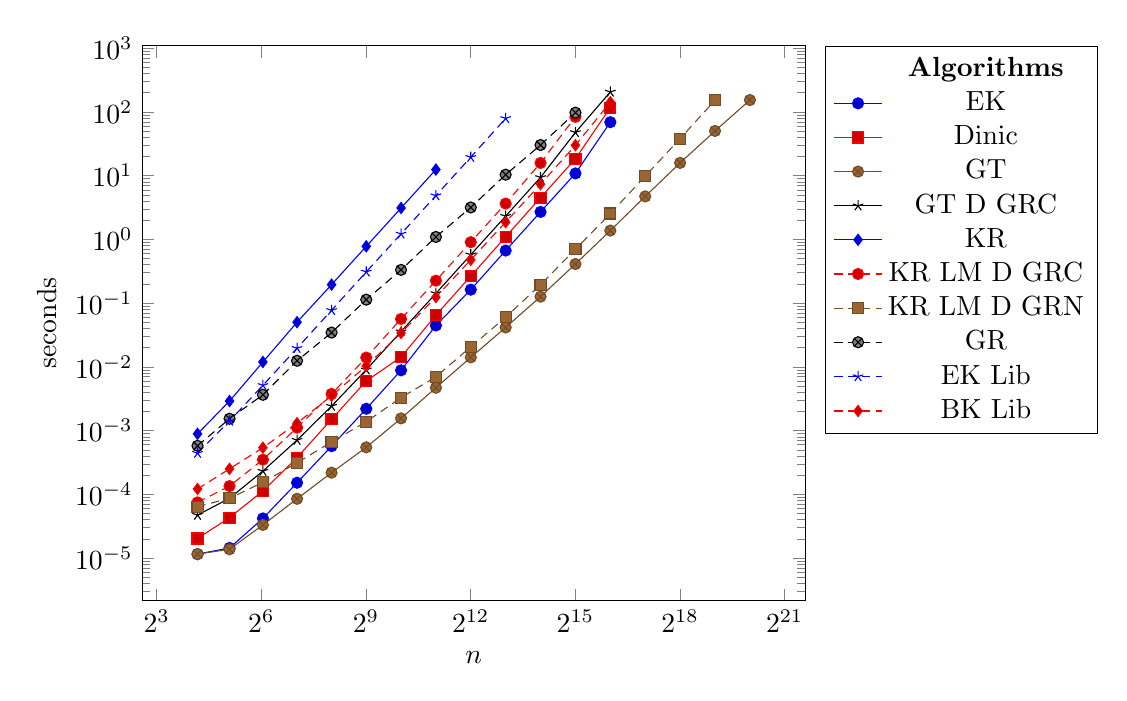
\begin{tikzpicture}
\begin{axis}[
    xlabel=$n$,ylabel=seconds,
    xmode=log,ymode=log,
    log basis x={2},
    legend style=
    {
        legend pos=outer north east
    },
    width=10cm
]
\addlegendimage{legend image code/.code=}
\legend{\textbf{Algorithms}, EK, Dinic, GT, GT D GRC, KR, KR LM D GRC, KR LM D GRN, GR, EK Lib, BK Lib}
\addplot table[x=n,y=value] {%EK
n value
18	1.15491E-05
34	1.44364E-05
66	4.19766E-05
130	0.000152249
258	0.000570682
514	0.002202887
1026	0.008838197
2050	0.0446577
4098	0.162670667
8194	0.668331333
16386	2.69851
32770	10.8331
65538	69.00813333
};
\addplot table[x=n,y=value] {%Dinic
n value
18	2.0322E-05
34	4.30871E-05
66	0.000113381
130	0.000376457
258	0.001508607
514	0.00600899
1026	0.014264533
2050	0.064598533
4098	0.265333667
8194	1.096893333
16386	4.517406667
32770	18.42716667
65538	116.604
};
\addplot table[x=n,y=value] {%GT
n value
18	1.15491E-05
34	1.37701E-05
66	3.32038E-05
130	8.51749E-05
258	0.000218989
514	0.000547029
1026	0.001555913
2050	0.004708267
4098	0.014102167
8194	0.041543667
16386	0.126403
32770	0.410714667
65538	1.375183333
131074	4.7243
262146	15.85233333
524290	50.24406667
1048578	153.437
};
\addplot table[x=n,y=value] {%GT D GRC
n value
18	4.73071E-05
34	8.68408E-05
66	0.000231983
130	0.000709607
258	0.002425103
514	0.009009903
1026	0.0358142
2050	0.142085333
4098	0.575261667
8194	2.315736667
16386	9.388776667
32770	47.68883333
65538	205.5886667
};
\addplot table[x=n,y=value] {%KR
n value
18	0.000889175
34	0.002908057
66	0.011943033
130	0.050249867
258	0.195147333
514	0.777756
1026	3.107726667
2050	12.4823
};
\addplot table[x=n,y=value] {%KR LM D GRC
n value
18	7.48474E-05
34	0.000134814
66	0.000350584
130	0.00111305
258	0.003765693
514	0.014000933
1026	0.0564863
2050	0.225324667
4098	0.904017333
8194	3.646476667
16386	15.8397
32770	83.65686667
};
\addplot table[x=n,y=value] {%KR LM D GRN
n value
18	6.41867E-05
34	8.66187E-05
66	0.00015447
130	0.000312605
258	0.000664521
514	0.001379017
1026	0.003295733
2050	0.006980693
4098	0.020601467
8194	0.0600087
16386	0.194730333
32770	0.69788
65538	2.548136667
131074	9.800743333
262146	38.14566667
524290	152.5736667
};
\addplot table[x=n,y=value] {%GR
n value
18	0.000578012
34	0.001536363
66	0.003647417
130	0.012470067
258	0.034521233
514	0.113386
1026	0.332325333
2050	1.092523333
4098	3.170253333
8194	10.35553333
16386	30.2229
32770	97.3555
};
\addplot table[x=n,y=value] {%EK Lib
n value
18	0.000443645
34	0.001415443
66	0.005145503
130	0.019632167
258	0.077202333
514	0.309274333
1026	1.21978
2050	4.860823333
4098	19.46263333
8194	79.22313333
};
\addplot table[x=n,y=value] {%BK Lib
n value
18	0.000121378
34	0.000251306
66	0.000539481
130	0.001310057
258	0.003520287
514	0.010349767
1026	0.0339719
2050	0.124275
4098	0.477602
8194	1.861176667
16386	7.34532
32770	29.98583333
65538	142.366
};
\end{axis}
\end{tikzpicture}
\caption{Best and worst results from the AK graphs}
\label{fig:AK_BW_Results}
\end{figure}


\begin{figure}[h]
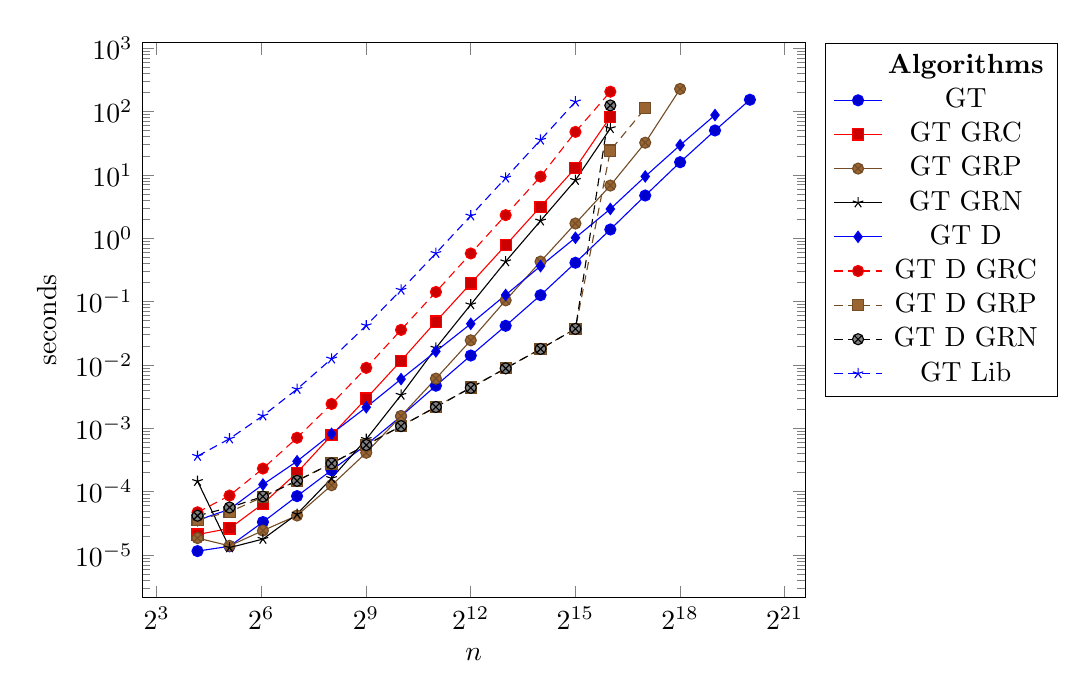
\begin{tikzpicture}
\begin{axis}[
    xlabel=$n$,ylabel=seconds,
    xmode=log,ymode=log,
    log basis x={2},
    legend style=
    {
        legend pos=outer north east
    },
    width=10cm
]
\addlegendimage{legend image code/.code=}
\legend{\textbf{Algorithms}, GT, GT GRC, GT GRP, GT GRN, GT D, GT D GRC, GT D GRP, GT D GRN, GT Lib}
\addplot table[x=n,y=value] {%GT
n value
18	1.15491E-05
34	1.37701E-05
66	3.32038E-05
130	8.51749E-05
258	0.000218989
514	0.000547029
1026	0.001555913
2050	0.004708267
4098	0.014102167
8194	0.041543667
16386	0.126403
32770	0.410714667
65538	1.375183333
131074	4.7243
262146	15.85233333
524290	50.24406667
1048578	153.437
};
\addplot table[x=n,y=value] {%GT GRC
n value
18	2.10994E-05
34	2.63187E-05
66	6.45197E-05
130	0.000200222
258	0.000779344
514	0.002955247
1026	0.011688167
2050	0.0483993
4098	0.193606
8194	0.774928333
16386	3.153233333
32770	12.85786667
65538	82.32676667
};
\addplot table[x=n,y=value] {%GT GRP
n value
18	1.85453E-05
34	1.39922E-05
66	2.43198E-05
130	4.20877E-05
258	0.000126596
514	0.000411993
1026	0.001565127
2050	0.006093057
4098	0.0244856
8194	0.104717
16386	0.428277667
32770	1.70907
65538	6.788133333
131074	32.18266667
262146	227.165
};
\addplot table[x=n,y=value] {%GT GRN
n value
18	0.000146252
34	1.31039E-05
66	0.000017879
130	4.43088E-05
258	0.00016291
514	0.000673739
1026	0.003355143
2050	0.018532733
4098	0.089804633
8194	0.429052667
16386	1.885126667
32770	8.247653333
65538	54.24016667
};
\addplot table[x=n,y=value] {%GT D
n value
18	3.54249E-05
34	5.28596E-05
66	0.000129928
130	0.00030261
258	0.000819102
514	0.002152143
1026	0.005989243
2050	0.016409467
4098	0.044628533
8194	0.127470333
16386	0.363211
32770	1.019396667
65538	2.897966667
131074	9.462753333
262146	29.41903333
524290	88.0256
};
\addplot table[x=n,y=value] {%GT D GRC
n value
18	4.73071E-05
34	8.68408E-05
66	0.000231983
130	0.000709607
258	0.002425103
514	0.009009903
1026	0.0358142
2050	0.142085333
4098	0.575261667
8194	2.315736667
16386	9.388776667
32770	47.68883333
65538	205.5886667
};
\addplot table[x=n,y=value] {%GT D GRP
n value
18	3.60912E-05
34	4.79734E-05
66	8.2621E-05
130	0.000149362
258	0.000279179
514	0.000546364
1026	0.00109295
2050	0.002178017
4098	0.00441367
8194	0.008896857
16386	0.017891767
32770	0.0374025
65538	24.21606667
131074	112.5863333
};
\addplot table[x=n,y=value] {%GT D GRN
n value
18	4.17547E-05
34	5.64132E-05
66	8.40646E-05
130	0.000148473
258	0.000279623
514	0.000545365
1026	0.001084287
2050	0.002170243
4098	0.00436003
8194	0.008836443
16386	0.0179194
32770	0.037174767
65538	124.819
};
\addplot table[x=n,y=value] {%GT Lib
n value
18	0.000364577
34	0.000685067
66	0.001577687
130	0.00415938
258	0.012518467
514	0.0419147
1026	0.152552
2050	0.579812333
4098	2.263826667
8194	8.971396667
16386	35.5501
32770	142.772
};
\end{axis}
\end{tikzpicture}
\caption{Goldberg and Tarjan results from the AK graphs}
\label{fig:AK_GT_ResultsAppendix}
\end{figure}


\begin{figure}[h]
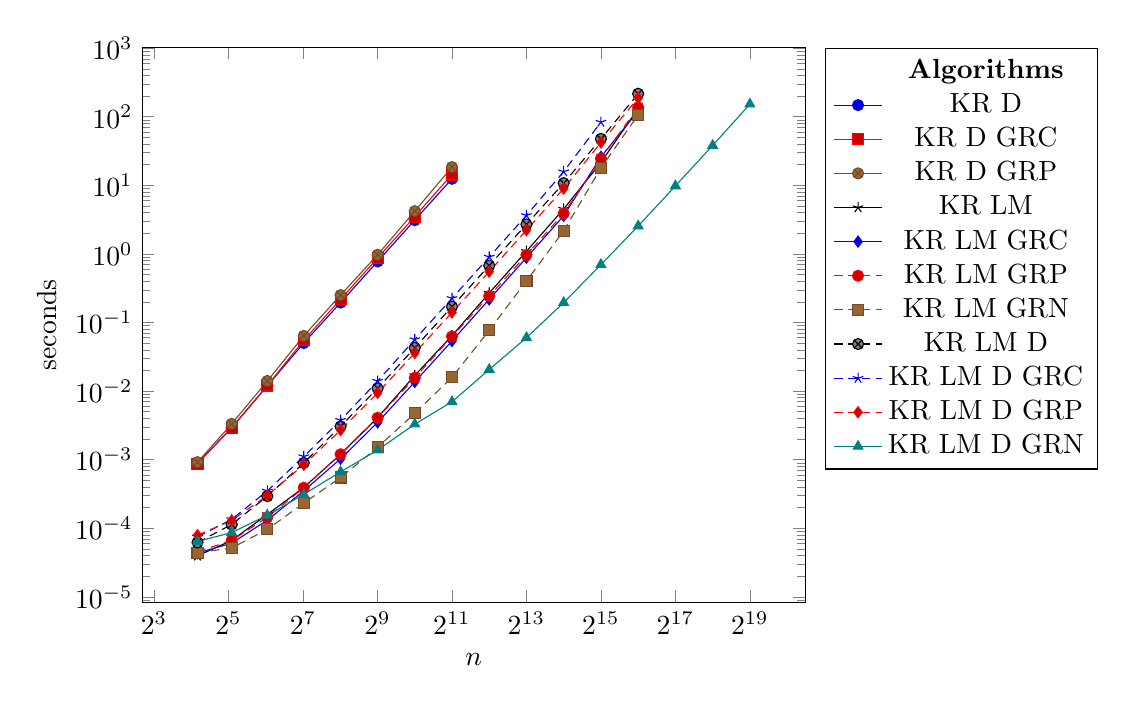
\begin{tikzpicture}
\begin{axis}[
    xlabel=$n$,ylabel=seconds,
    xmode=log,ymode=log,
    log basis x={2},
    legend style=
    {
        legend pos=outer north east
    },
    width=10cm
]
\addlegendimage{legend image code/.code=}
\legend{\textbf{Algorithms}, KR D, KR D GRC, KR D GRP, KR LM, KR LM GRC, KR LM GRP, KR LM GRN, KR LM D, KR LM D GRC, KR LM D GRP, KR LM D GRN}
\addplot table[x=n,y=value] {%KR
n value
18	0.000889175
34	0.002908057
66	0.011943033
130	0.050249867
258	0.195147333
514	0.777756
1026	3.107726667
2050	12.4823
};
\addplot table[x=n,y=value] {%KR GRC
n value
18	0.000875735
34	0.002938147
66	0.0120653
130	0.054935867
258	0.218274
514	0.872710333
1026	3.5095
2050	14.403
};
\addplot table[x=n,y=value] {%KR GRP
n value
18	0.000919492
34	0.00332838
66	0.014040333
130	0.0638248
258	0.251151333
514	0.971965333
1026	4.19931
2050	18.4658
};
\addplot table[x=n,y=value] {%KR LM
n value
18	3.95337E-05
34	6.66298E-05
66	0.000158912
130	0.000393449
258	0.00119856
514	0.00412505
1026	0.016918733
2050	0.064206667
4098	0.268975333
8194	1.09322
16386	4.51368
32770	21.53186667
65538	131.6553333
};
\addplot table[x=n,y=value] {%KR LM GRC
n value
18	4.34204E-05
34	6.07442E-05
66	0.000131261
130	0.000351139
258	0.001029877
514	0.00350173
1026	0.013609367
2050	0.0537659
4098	0.217405
8194	0.881691
16386	3.602213333
32770	26.04033333
65538	120.6886667
};
\addplot table[x=n,y=value] {%KR LM GRP
n value
18	4.57524E-05
34	6.62967E-05
66	0.000144697
130	0.000389451
258	0.00119834
514	0.00407752
1026	0.015643533
2050	0.062576267
4098	0.243189667
8194	0.966999333
16386	3.8901
32770	24.61043333
65538	136.8136667
};
\addplot table[x=n,y=value] {%KR LM GRN
n value
18	4.38646E-05
34	5.16381E-05
66	9.65021E-05
130	0.000232649
258	0.000549696
514	0.00151394
1026	0.00474304
2050	0.0158961
4098	0.0767171
8194	0.402905667
16386	2.16554
32770	17.93576667
65538	106.1156667
};
\addplot table[x=n,y=value] {%KR LM D
n value
18	6.21878E-05
34	0.000113493
66	0.000293837
130	0.000895949
258	0.003054753
514	0.010999333
1026	0.0427871
2050	0.170356
4098	0.676120333
8194	2.693893333
16386	10.74853333
32770	47.54073333
65538	216.514
};
\addplot table[x=n,y=value] {%KR LM D GRC
n value
18	7.48474E-05
34	0.000134814
66	0.000350584
130	0.00111305
258	0.003765693
514	0.014000933
1026	0.0564863
2050	0.225324667
4098	0.904017333
8194	3.646476667
16386	15.8397
32770	83.65686667
};
\addplot table[x=n,y=value] {%KR LM D GRP
n value
18	7.94004E-05
34	0.000130039
66	0.000300056
130	0.000844977
258	0.002696287
514	0.009420677
1026	0.035984667
2050	0.140029
4098	0.551803333
8194	2.21699
16386	8.955463333
32770	42.12056667
65538	186.7876667
};
\addplot[mark=triangle*, teal] table[x=n,y=value] {%KR LM D GRN
n value
18	6.41867E-05
34	8.66187E-05
66	0.00015447
130	0.000312605
258	0.000664521
514	0.001379017
1026	0.003295733
2050	0.006980693
4098	0.020601467
8194	0.0600087
16386	0.194730333
32770	0.69788
65538	2.548136667
131074	9.800743333
262146	38.14566667
524290	152.5736667
};
\end{axis}
\end{tikzpicture}
\caption{King and Rao results from the AK graphs}
\label{fig:AK_KR_ResultsAppendix}
\end{figure}

%-----------------------------------------------------------------------------------------------------------
\clearpage


\subsection{Results from GenRmf long graphs}
\begin{figure}[h]
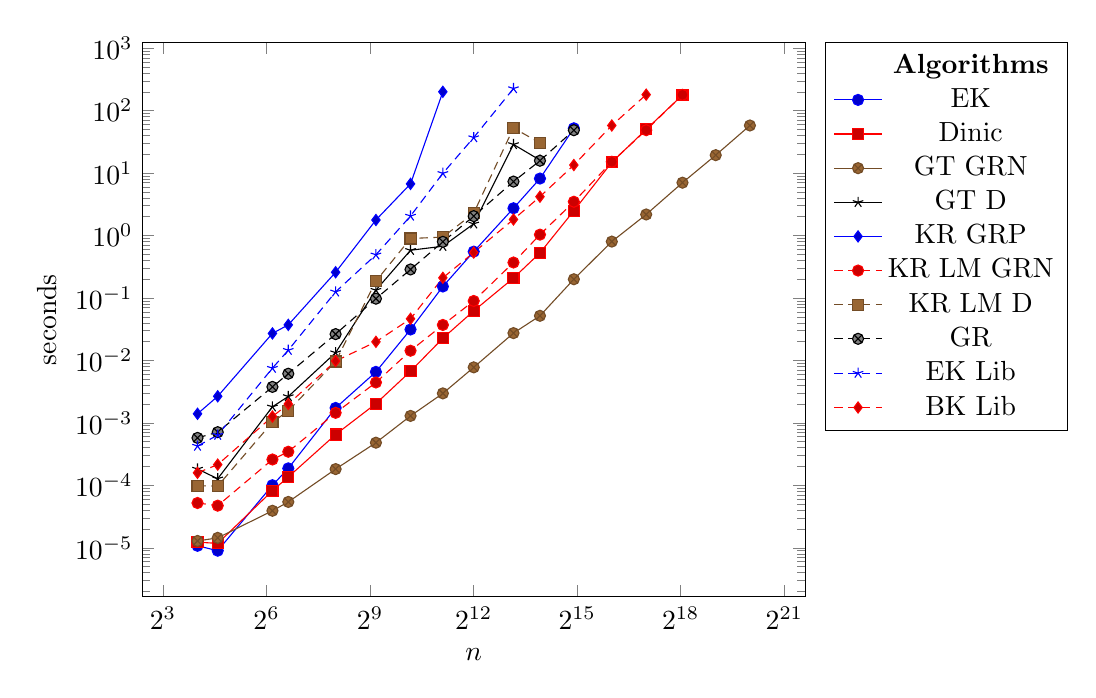
\begin{tikzpicture}
\begin{axis}[
    xlabel=$n$,ylabel=seconds,
    xmode=log,ymode=log,
    log basis x={2},
    legend style=
    {
        legend pos=outer north east
    },
    width=10cm
]
\addlegendimage{legend image code/.code=}
\legend{\textbf{Algorithms}, EK, Dinic, GT GRN, GT D, KR GRP, KR LM GRN, KR LM D, GR, EK Lib, BK Lib}
\addplot table[x=n,y=value] {%EK
n value
16	1.07718E-05
24	8.99499E-06
72	0.0001005
99	0.000187118
256	0.001736033
575	0.006561127
1152	0.031316167
2205	0.152855333
4096	0.552244333
9100	2.735133333
15488	8.1725
30589	52.13166667
};
\addplot table[x=n,y=value] {%Dinic
n value
16	1.23265E-05
24	1.17712E-05
72	8.21765E-05
99	0.000136146
256	0.000651637
575	0.002034203
1152	0.006705713
2205	0.022681033
4096	0.0621048
9100	0.208537333
15488	0.527127667
30589	2.491446667
65536	14.86433333
130682	50.06016667
270848	177.8626667
};
\addplot table[x=n,y=value] {%GT GRN
n value
16	1.28818E-05
24	1.44365E-05
72	3.92005E-05
99	5.43033E-05
256	0.000182232
575	0.000482289
1152	0.001294393
2205	0.002970023
4096	0.00775149
9100	0.0273884
15488	0.051847533
30589	0.199656667
65536	0.799864667
130682	2.173773333
270848	7.017736667
527796	19.36696667
1048576	57.80963333
};
\addplot table[x=n,y=value] {%GT D
n value
16	0.000182899
24	0.000127707
72	0.001811667
99	0.002649647
256	0.01333294
575	0.133493
1152	0.581190667
2205	0.673778667
4096	1.540246667
9100	28.75023333
15488	16.11123333
};
\addplot table[x=n,y=value] {%KR GRP
n value
16	0.00139845
24	0.002666637
72	0.0271098
99	0.037121367
256	0.258182333
575	1.773686667
1152	6.72207
2205	200.141
};
\addplot table[x=n,y=value] {%KR LM GRN
n value
16	5.21933E-05
24	4.73072E-05
72	0.000259523
99	0.000345365
256	0.001449643
575	0.00443921
1152	0.014312
2205	0.037018833
4096	0.089594333
9100	0.369817
15488	1.033306667
30589	3.473556667
65536	15.1593
130682	48.64013333
270848	178.9876667
};
\addplot table[x=n,y=value] {%KR LM D
n value
16	9.88343E-05
24	9.73907E-05
72	0.001024097
99	0.001562027
256	0.009612567
575	0.186065333
1152	0.896549
2205	0.943830667
4096	2.28156
9100	52.7981
15488	30.36093333
};
\addplot table[x=n,y=value] {%GR
n value
16	0.000575236
24	0.000710605
72	0.003772567
99	0.00613292
256	0.026391333
575	0.097505533
1152	0.286460667
2205	0.792706667
4096	2.04237
9100	7.310506667
15488	15.76233333
30589	48.56896667
};
\addplot table[x=n,y=value] {%EK Lib
n value
16	0.000425988
24	0.000638093
72	0.007533857
99	0.014606733
256	0.125504667
575	0.491983667
1152	2.055623333
2205	9.923236667
4096	37.06083333
9100	225.8106667
};
\addplot table[x=n,y=value] {%BK Lib
n value
16	0.00015869
24	0.000214993
72	0.00126475
99	0.002003343
256	0.009785063
575	0.019859533
1152	0.0464782
2205	0.210524
4096	0.53478
9100	1.80975
15488	4.18626
30589	13.45136667
65536	57.83356667
130682	180.1683333
};
\end{axis}
\end{tikzpicture}
\caption{Best and worst results from the GenRmf long graphs}
\label{fig:GenRmf long_BW_Results}
\end{figure}


\begin{figure}[h]
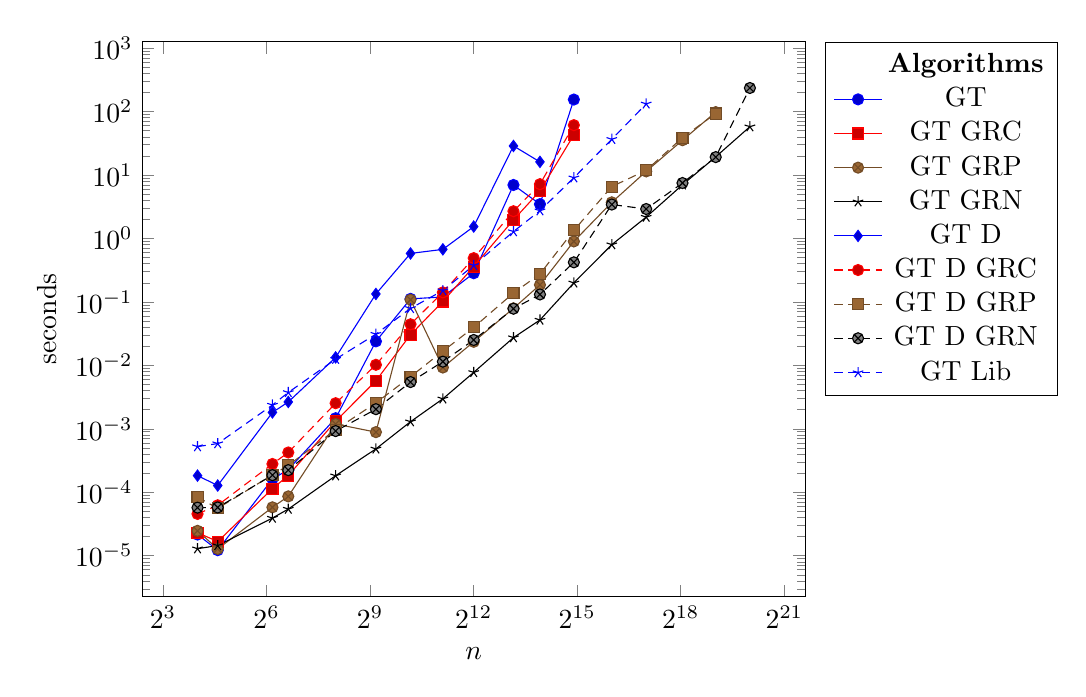
\begin{tikzpicture}
\begin{axis}[
    xlabel=$n$,ylabel=seconds,
    xmode=log,ymode=log,
    log basis x={2},
    legend style=
    {
        legend pos=outer north east
    },
    width=10cm
]
\addlegendimage{legend image code/.code=}
\legend{\textbf{Algorithms}, GT, GT GRC, GT GRP, GT GRN, GT D, GT D GRC, GT D GRP, GT D GRN, GT Lib}
\addplot table[x=n,y=value] {%GT
n value
16	2.15436E-05
24	1.22154E-05
72	0.000161133
99	0.00022754
256	0.001468293
575	0.023901133
1152	0.111713
2205	0.119803
4096	0.28348
9100	6.972716667
15488	3.47428
30589	154.8906667
};
\addplot table[x=n,y=value] {%GT GRC
n value
16	2.30983E-05
24	1.66574E-05
72	0.000114048
99	0.000183232
256	0.00131771
575	0.005709937
1152	0.030467267
2205	0.101588
4096	0.360189
9100	1.96376
15488	5.613036667
30589	42.95033333
};
\addplot table[x=n,y=value] {%GT GRP
n value
16	2.4653E-05
24	1.27707E-05
72	5.78567E-05
99	8.60632E-05
256	0.001188007
575	0.000886396
1152	0.108298
2205	0.009246077
4096	0.0235188
9100	0.079296967
15488	0.185714333
30589	0.899061333
65536	3.712403333
130682	11.41563333
270848	35.41273333
527796	98.1075
};
\addplot table[x=n,y=value] {%GT GRN
n value
16	1.28818E-05
24	1.44365E-05
72	3.92005E-05
99	5.43033E-05
256	0.000182232
575	0.000482289
1152	0.001294393
2205	0.002970023
4096	0.00775149
9100	0.0273884
15488	0.051847533
30589	0.199656667
65536	0.799864667
130682	2.173773333
270848	7.017736667
527796	19.36696667
1048576	57.80963333
};
\addplot table[x=n,y=value] {%GT D
n value
16	0.000182899
24	0.000127707
72	0.001811667
99	0.002649647
256	0.01333294
575	0.133493
1152	0.581190667
2205	0.673778667
4096	1.540246667
9100	28.75023333
15488	16.11123333
};
\addplot table[x=n,y=value] {%GT D GRC
n value
16	4.55303E-05
24	6.22988E-05
72	0.000279179
99	0.000423655
256	0.00253193
575	0.010205033
1152	0.044468633
2205	0.141443667
4096	0.490048
9100	2.690203333
15488	7.183683333
30589	61.1455
};
\addplot table[x=n,y=value] {%GT D GRP
n value
16	8.40646E-05
24	5.57469E-05
72	0.000188007
99	0.000264631
256	0.000967909
575	0.002560693
1152	0.006632443
2205	0.016727867
4096	0.039698667
9100	0.138222667
15488	0.27566
30589	1.342566667
65536	6.573553333
130682	11.86123333
270848	38.87526667
527796	93.12866667
};
\addplot table[x=n,y=value] {%GT D GRN
n value
16	5.71906E-05
24	5.75237E-05
72	0.000186008
99	0.000223099
256	0.000920491
575	0.002039097
1152	0.005452093
2205	0.011442267
4096	0.025133533
9100	0.078167533
15488	0.131162333
30589	0.420732667
65536	3.42981
130682	2.91399
270848	7.486506667
527796	19.16753333
1048576	235.5196667
};
\addplot table[x=n,y=value] {%GT Lib
n value
16	0.000524045
24	0.000584789
72	0.002370587
99	0.003742273
256	0.012512867
575	0.031066333
1152	0.079139833
2205	0.151054
4096	0.376943
9100	1.286306667
15488	2.73918
30589	9.066496667
65536	36.64306667
130682	132.3713333
};
\end{axis}
\end{tikzpicture}
\caption{Goldberg and Tarjan results from the GenRmf long graphs}
\label{fig:GenRmf long_GT_ResultsAppendix}
\end{figure}


\begin{figure}[h]
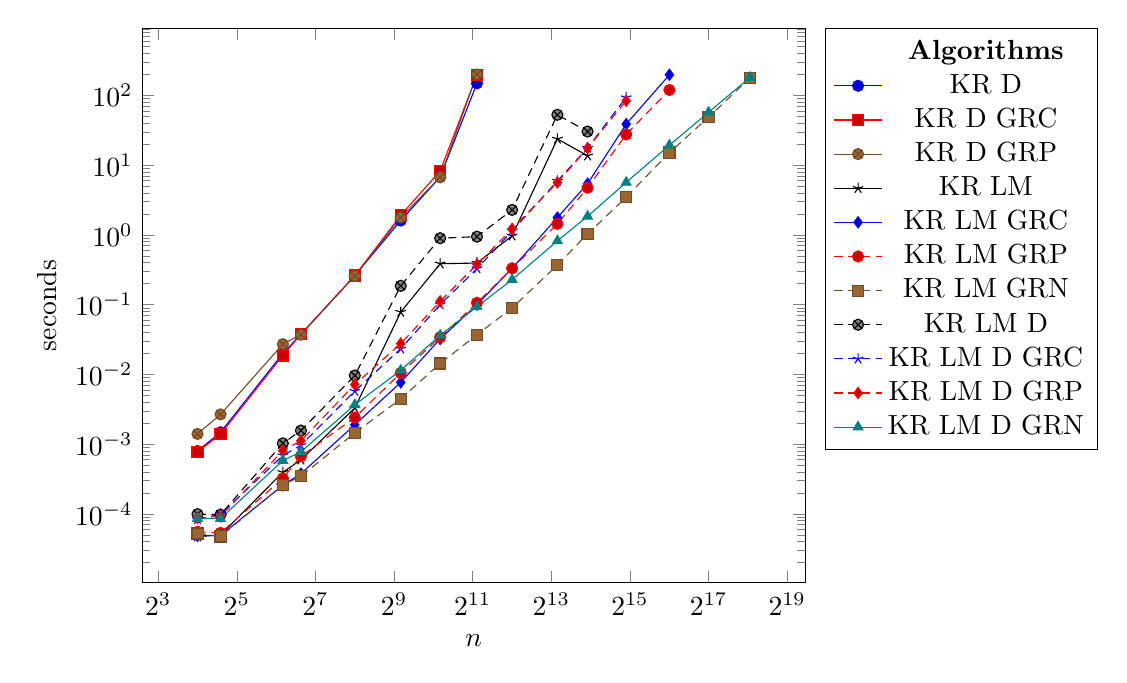
\begin{tikzpicture}
\begin{axis}[
    xlabel=$n$,ylabel=seconds,
    xmode=log,ymode=log,
    log basis x={2},
    legend style=
    {
        legend pos=outer north east
    },
    width=10cm
]
\addlegendimage{legend image code/.code=}
\legend{\textbf{Algorithms}, KR D, KR D GRC, KR D GRP, KR LM, KR LM GRC, KR LM GRP, KR LM GRN, KR LM D, KR LM D GRC, KR LM D GRP, KR LM D GRN}
\addplot table[x=n,y=value] {%KR
n value
16	0.000795004
24	0.00147618
72	0.019901867
99	0.037501367
256	0.260456667
575	1.606663333
1152	6.740186667
2205	149.337
};
\addplot table[x=n,y=value] {%KR GRC
n value
16	0.000769905
24	0.001389337
72	0.018663067
99	0.0377529
256	0.261381
575	1.908376667
1152	8.252073333
2205	197.4756667
};
\addplot table[x=n,y=value] {%KR GRP
n value
16	0.00139845
24	0.002666637
72	0.0271098
99	0.037121367
256	0.258182333
575	1.773686667
1152	6.72207
2205	200.141
};
\addplot table[x=n,y=value] {%KR LM
n value
16	4.70851E-05
24	4.97503E-05
72	0.000394004
99	0.000594782
256	0.003290843
575	0.078265033
1152	0.385737667
2205	0.395114667
4096	0.969813
9100	23.78033333
15488	13.6657
};
\addplot table[x=n,y=value] {%KR LM GRC
n value
16	4.81955E-05
24	4.90839E-05
72	0.000255858
99	0.000376681
256	0.001889957
575	0.007676197
1152	0.0321853
2205	0.099800333
4096	0.331238
9100	1.773373333
15488	5.421613333
30589	38.8194
65536	197.752
};
\addplot table[x=n,y=value] {%KR LM GRP
n value
16	5.53027E-05
24	5.31928E-05
72	0.000322266
99	0.000671628
256	0.002406003
575	0.010445347
1152	0.034050267
2205	0.10638
4096	0.331282667
9100	1.439603333
15488	4.751253333
30589	27.6015
65536	119.7773333
};
\addplot table[x=n,y=value] {%KR LM GRN
n value
16	5.21933E-05
24	4.73072E-05
72	0.000259523
99	0.000345365
256	0.001449643
575	0.00443921
1152	0.014312
2205	0.037018833
4096	0.089594333
9100	0.369817
15488	1.033306667
30589	3.473556667
65536	15.1593
130682	48.64013333
270848	178.9876667
};
\addplot table[x=n,y=value] {%KR LM D
n value
16	9.88343E-05
24	9.73907E-05
72	0.001024097
99	0.001562027
256	0.009612567
575	0.186065333
1152	0.896549
2205	0.943830667
4096	2.28156
9100	52.7981
15488	30.36093333
};
\addplot table[x=n,y=value] {%KR LM D GRC
n value
16	8.31763E-05
24	9.87233E-05
72	0.000685843
99	0.000960468
256	0.00575304
575	0.023246133
1152	0.100415667
2205	0.328566333
4096	1.139136667
9100	5.931156667
15488	17.6933
30589	93.37536667
};
\addplot table[x=n,y=value] {%KR LM D GRP
n value
16	8.69519E-05
24	9.19491E-05
72	0.000803777
99	0.001117273
256	0.007166817
575	0.027587633
1152	0.111327333
2205	0.376117333
4096	1.221456667
9100	5.651543333
15488	17.5763
30589	83.79273333
};
\addplot[mark=triangle*, teal] table[x=n,y=value] {%KR LM D GRN
n value
16	8.53971E-05
24	8.53972E-05
72	0.000580235
99	0.000774794
256	0.00366275
575	0.011421333
1152	0.036280633
2205	0.0934643
4096	0.228176333
9100	0.820808667
15488	1.847203333
30589	5.658126667
65536	19.2994
130682	57.2744
270848	180.989
};
\end{axis}
\end{tikzpicture}
\caption{King and Rao results from the GenRmf long graphs}
\label{fig:GenRmf long_KR_ResultsAppendix}
\end{figure}

%-----------------------------------------------------------------------------------------------------------
\clearpage


\subsection{Results from GenRmf flat graphs}
\begin{figure}[h]
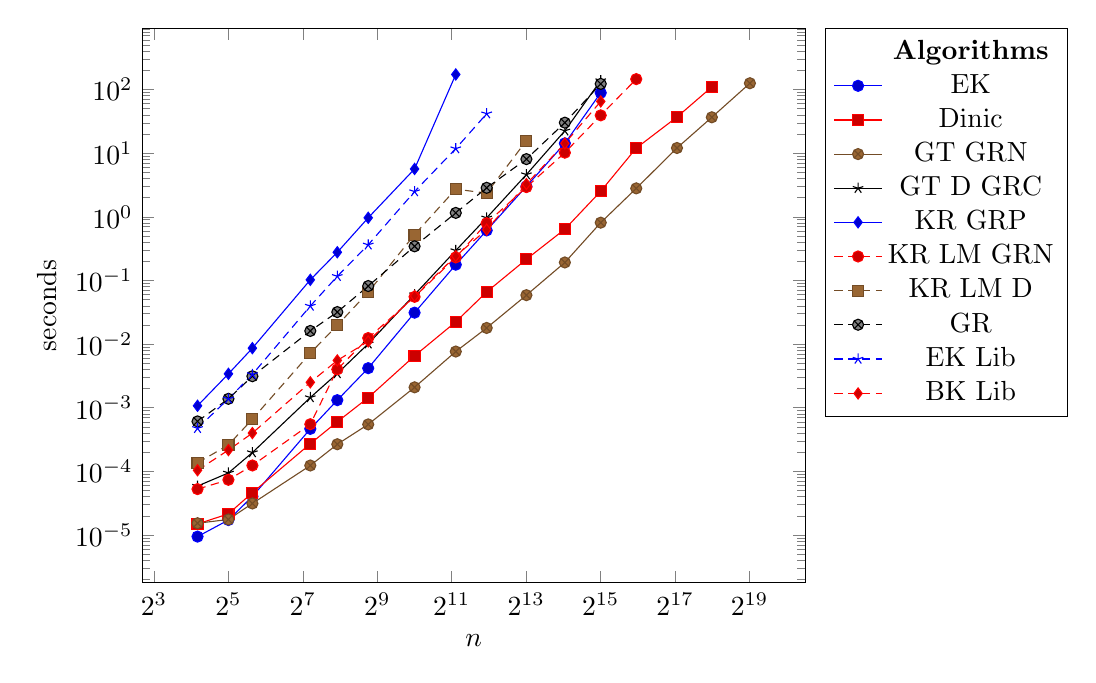
\begin{tikzpicture}
\begin{axis}[
    xlabel=$n$,ylabel=seconds,
    xmode=log,ymode=log,
    log basis x={2},
    legend style=
    {
        legend pos=outer north east
    },
    width=10cm
]
\addlegendimage{legend image code/.code=}
\legend{\textbf{Algorithms}, EK, Dinic, GT GRN, GT D GRC, KR GRP, KR LM GRN, KR LM D, GR, EK Lib, BK Lib}
\addplot table[x=n,y=value] {%EK
n value
18	9.4392E-06
32	1.72126E-05
50	4.03109E-05
147	0.000465408
243	0.001316157
432	0.00418523
1024	0.031191967
2205	0.176996333
3920	0.611422
8214	3.014606667
16807	14.2787
32768	88.94956667
};
\addplot table[x=n,y=value] {%Dinic
n value
18	1.48806E-05
32	2.15436E-05
50	4.61965E-05
147	0.000272404
243	0.000601443
432	0.001440867
1024	0.00653603
2205	0.022350033
3920	0.0660307
8214	0.215527667
16807	0.640137667
32768	2.524353333
63504	12.02686667
135531	36.99756667
259308	109.8443333
};
\addplot table[x=n,y=value] {%GT GRN
n value
18	1.53249E-05
32	1.75459E-05
50	0.000031316
147	0.00012371
243	0.000266963
432	0.000547475
1024	0.002093063
2205	0.007644327
3920	0.017937867
8214	0.0587656
16807	0.191883
32768	0.809820333
63504	2.801476667
135531	12.06703333
259308	36.68086667
526904	125.7226667
};
\addplot table[x=n,y=value] {%GT D GRC
n value
18	5.87453E-05
32	9.45034E-05
50	0.000197669
147	0.001447867
243	0.003451533
432	0.010111967
1024	0.059864533
2205	0.295727
3920	0.963905
8214	4.61783
16807	22.47756667
32768	138.508
};
\addplot table[x=n,y=value] {%KR GRP
n value
18	0.001074073
32	0.003409223
50	0.008633337
147	0.102404
243	0.277406
432	0.965820667
1024	5.656363333
2205	172.7583333
};
\addplot table[x=n,y=value] {%KR LM GRN
n value
18	5.26376E-05
32	0.000073737
50	0.00012382
147	0.000550917
243	0.004011667
432	0.012442333
1024	0.055324933
2205	0.230305333
3920	0.794109
8214	2.930473333
16807	10.18923333
32768	39.32803333
63504	145.8696667
};
\addplot table[x=n,y=value] {%KR LM D
n value
18	0.000136036
32	0.000260523
50	0.000661301
147	0.007218563
243	0.019773733
432	0.0653776
1024	0.525896
2205	2.72503
3920	2.35291
8214	15.7247
};
\addplot table[x=n,y=value] {%GR
n value
18	0.000610216
32	0.00138123
50	0.003127593
147	0.016109833
243	0.031885167
432	0.0818089
1024	0.343863333
2205	1.153163333
3920	2.85746
8214	8.068233333
16807	30.1861
32768	122.866
};
\addplot table[x=n,y=value] {%EK Lib
n value
18	0.000475183
32	0.001380687
50	0.00333872
147	0.039699067
243	0.116443333
432	0.363236333
1024	2.4961
2205	11.80336667
3920	41.74636667
};
\addplot table[x=n,y=value] {%BK Lib
n value
18	0.000104054
32	0.000215992
50	0.00039978
147	0.002510063
243	0.005535177
432	0.0110366
1024	0.0570666
2205	0.242166333
3920	0.629387
8214	3.27575
16807	14.24913333
32768	65.0965
};
\end{axis}
\end{tikzpicture}
\caption{Best and worst results from the GenRmf flat graphs}
\label{fig:GenRmf flat_BW_Results}
\end{figure}


\begin{figure}[h]
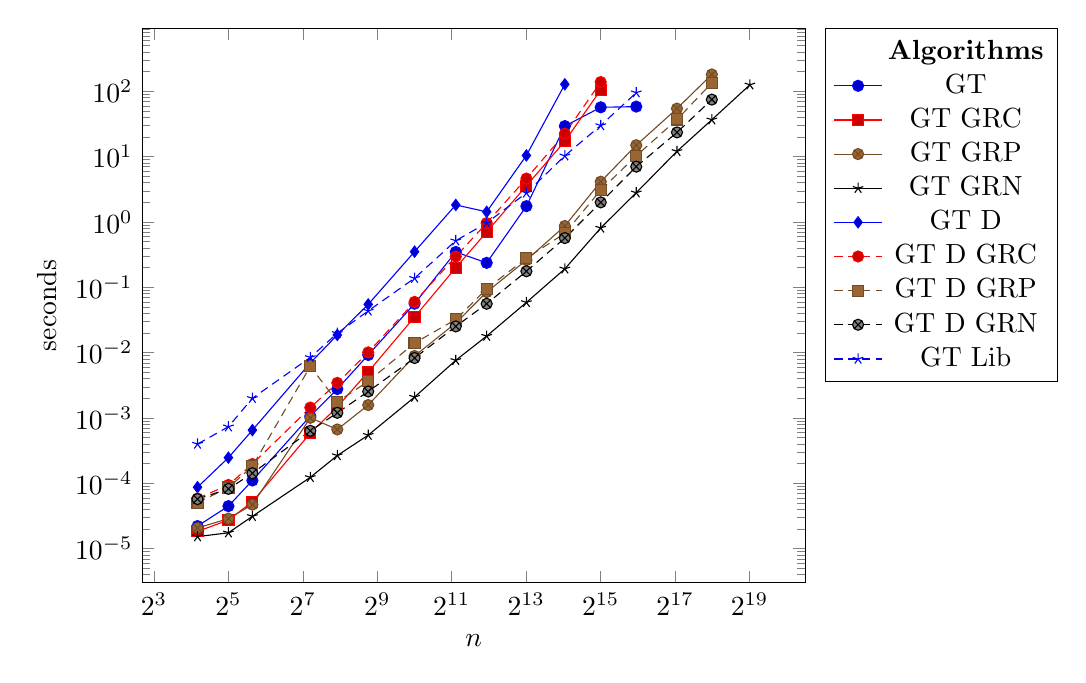
\begin{tikzpicture}
\begin{axis}[
    xlabel=$n$,ylabel=seconds,
    xmode=log,ymode=log,
    log basis x={2},
    legend style=
    {
        legend pos=outer north east
    },
    width=10cm
]
\addlegendimage{legend image code/.code=}
\legend{\textbf{Algorithms}, GT, GT GRC, GT GRP, GT GRN, GT D, GT D GRC, GT D GRP, GT D GRN, GT Lib}
\addplot table[x=n,y=value] {%GT
n value
18	2.22099E-05
32	4.48639E-05
50	0.000110827
147	0.001072623
243	0.002777677
432	0.009227643
1024	0.056178767
2205	0.347710667
3920	0.236927
8214	1.74571
16807	29.33203333
32768	56.85273333
63504	58.28513333
};
\addplot table[x=n,y=value] {%GT GRC
n value
18	1.84342E-05
32	2.74292E-05
50	5.23042E-05
147	0.000586896
243	0.001477067
432	0.00509139
1024	0.035166767
2205	0.199472
3920	0.702958333
8214	3.58601
16807	17.21576667
32768	105.3156667
};
\addplot table[x=n,y=value] {%GT GRP
n value
18	2.07662E-05
32	2.88728E-05
50	4.7307E-05
147	0.001008216
243	0.000668406
432	0.001579343
1024	0.008907267
2205	0.0284375
3920	0.084576833
8214	0.260927667
16807	0.868911
32768	4.137436667
63504	14.96233333
135531	54.3359
259308	181.0383333
};
\addplot table[x=n,y=value] {%GT GRN
n value
18	1.53249E-05
32	1.75459E-05
50	0.000031316
147	0.00012371
243	0.000266963
432	0.000547475
1024	0.002093063
2205	0.007644327
3920	0.017937867
8214	0.0587656
16807	0.191883
32768	0.809820333
63504	2.801476667
135531	12.06703333
259308	36.68086667
526904	125.7226667
};
\addplot table[x=n,y=value] {%GT D
n value
18	8.7396E-05
32	0.000247641
50	0.000652417
147	0.0069717
243	0.018692567
432	0.054880833
1024	0.351534
2205	1.823923333
3920	1.4308
8214	10.43303333
16807	127.9706667
};
\addplot table[x=n,y=value] {%GT D GRC
n value
18	5.87453E-05
32	9.45034E-05
50	0.000197669
147	0.001447867
243	0.003451533
432	0.010111967
1024	0.059864533
2205	0.295727
3920	0.963905
8214	4.61783
16807	22.47756667
32768	138.508
};
\addplot table[x=n,y=value] {%GT D GRP
n value
18	5.07497E-05
32	8.62856E-05
50	0.000182565
147	0.00619224
243	0.00176569
432	0.003644983
1024	0.014012367
2205	0.032288
3920	0.095217433
8214	0.279258333
16807	0.672308333
32768	3.07767
63504	10.2616
135531	37.05286667
259308	134.3013333
};
\addplot table[x=n,y=value] {%GT D GRN
n value
18	5.74127E-05
32	8.23989E-05
50	0.000143032
147	0.000637869
243	0.001202003
432	0.00254581
1024	0.008284307
2205	0.025236567
3920	0.056017433
8214	0.176041667
16807	0.567211
32768	1.995766667
63504	7.020556667
135531	23.4784
259308	74.6085
};
\addplot table[x=n,y=value] {%GT Lib
n value
18	0.000400113
32	0.000736262
50	0.00200534
147	0.008467563
243	0.019826867
432	0.043577133
1024	0.137993667
2205	0.516753333
3920	0.966842
8214	2.78562
16807	10.30583333
32768	29.97566667
63504	95.17936667
};
\end{axis}
\end{tikzpicture}
\caption{Goldberg and Tarjan results from the GenRmf flat graphs}
\label{fig:GenRmf flat_GT_Results}
\end{figure}


\begin{figure}[h]
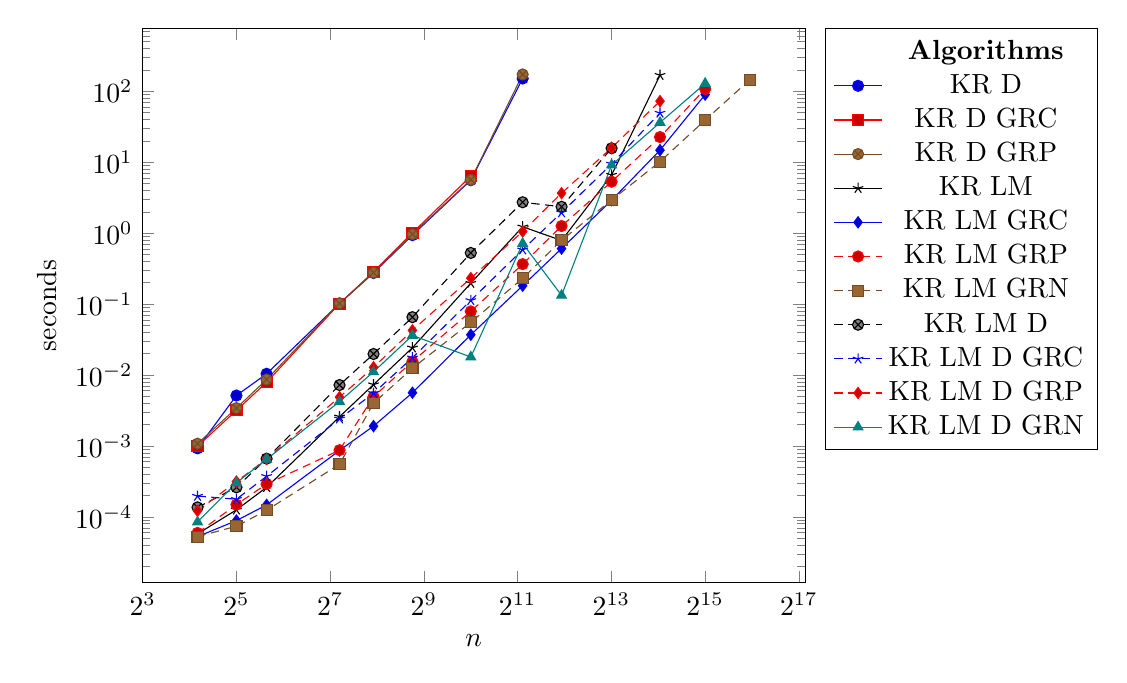
\begin{tikzpicture}
\begin{axis}[
    xlabel=$n$,ylabel=seconds,
    xmode=log,ymode=log,
    log basis x={2},
    legend style=
    {
        legend pos=outer north east
    },
    width=10cm
]
\addlegendimage{legend image code/.code=}
\legend{\textbf{Algorithms}, KR D, KR D GRC, KR D GRP, KR LM, KR LM GRC, KR LM GRP, KR LM GRN, KR LM D, KR LM D GRC, KR LM D GRP, KR LM D GRN}
\addplot table[x=n,y=value] {%KR
n value
18	0.000924822
32	0.005135713
50	0.010398667
147	0.1019604
243	0.274302333
432	0.936981667
1024	5.575076667
2205	151.3853333
};
\addplot table[x=n,y=value] {%KR GRC
n value
18	0.000991894
32	0.0031699
50	0.00789183
147	0.101455
243	0.285877333
432	1.00962
1024	6.366356667
};
\addplot table[x=n,y=value] {%KR GRP
n value
18	0.001074073
32	0.003409223
50	0.008633337
147	0.102404
243	0.277406
432	0.965820667
1024	5.656363333
2205	172.7583333
};
\addplot table[x=n,y=value] {%KR LM
n value
18	5.74127E-05
32	0.000125597
50	0.000260411
147	0.002579683
243	0.0073245
432	0.024196833
1024	0.197125667
2205	1.23007
3920	0.787139667
8214	6.59962
16807	168.589
};
\addplot table[x=n,y=value] {%KR LM GRC
n value
18	5.26375E-05
32	8.85064E-05
50	0.000147363
147	0.000863189
243	0.001903393
432	0.00562644
1024	0.036906367
2205	0.181411333
3920	0.605830667
8214	2.91064
16807	14.7904
32768	89.8431
};
\addplot table[x=n,y=value] {%KR LM GRP
n value
18	5.93005E-05
32	0.000149029
50	0.000290284
147	0.000871407
243	0.00495037
432	0.015484133
1024	0.078886133
2205	0.365700333
3920	1.26005
8214	5.312396667
16807	22.63123333
32768	107.989
};
\addplot table[x=n,y=value] {%KR LM GRN
n value
18	5.26376E-05
32	0.000073737
50	0.00012382
147	0.000550917
243	0.004011667
432	0.012442333
1024	0.055324933
2205	0.230305333
3920	0.794109
8214	2.930473333
16807	10.18923333
32768	39.32803333
63504	145.8696667
};
\addplot table[x=n,y=value] {%KR LM D
n value
18	0.000136036
32	0.000260523
50	0.000661301
147	0.007218563
243	0.019773733
432	0.0653776
1024	0.525896
2205	2.72503
3920	2.35291
8214	15.7247
};
\addplot table[x=n,y=value] {%KR LM D GRC
n value
18	0.000196224
32	0.000177235
50	0.000373349
147	0.002416107
243	0.005545263
432	0.017499567
1024	0.112657
2205	0.583763667
3920	1.945043333
8214	9.460863333
16807	49.42546667
};
\addplot table[x=n,y=value] {%KR LM D GRP
n value
18	0.000121488
32	0.000314382
50	0.00065486
147	0.00486675
243	0.0128281
432	0.042627733
1024	0.232225
2205	1.053173333
3920	3.663543333
8214	15.96356667
16807	72.6246
};
\addplot[mark=triangle*, teal] table[x=n,y=value] {%KR LM D GRN
n value
18	8.47309E-05
32	0.000302277
50	0.000648308
147	0.00421978
243	0.0110721
432	0.036097033
1024	0.017925533
2205	0.714243333
3920	0.132640667
8214	9.112416667
16807	36.27683333
32768	128.902
};
\end{axis}
\end{tikzpicture}
\caption{King and Rao results from the GenRmf flat graphs}
\label{fig:GenRmf flat_KR_Results}
\end{figure}

%-----------------------------------------------------------------------------------------------------------
\clearpage


\subsection{Results from GenRmf square graphs}
\begin{figure}[h]
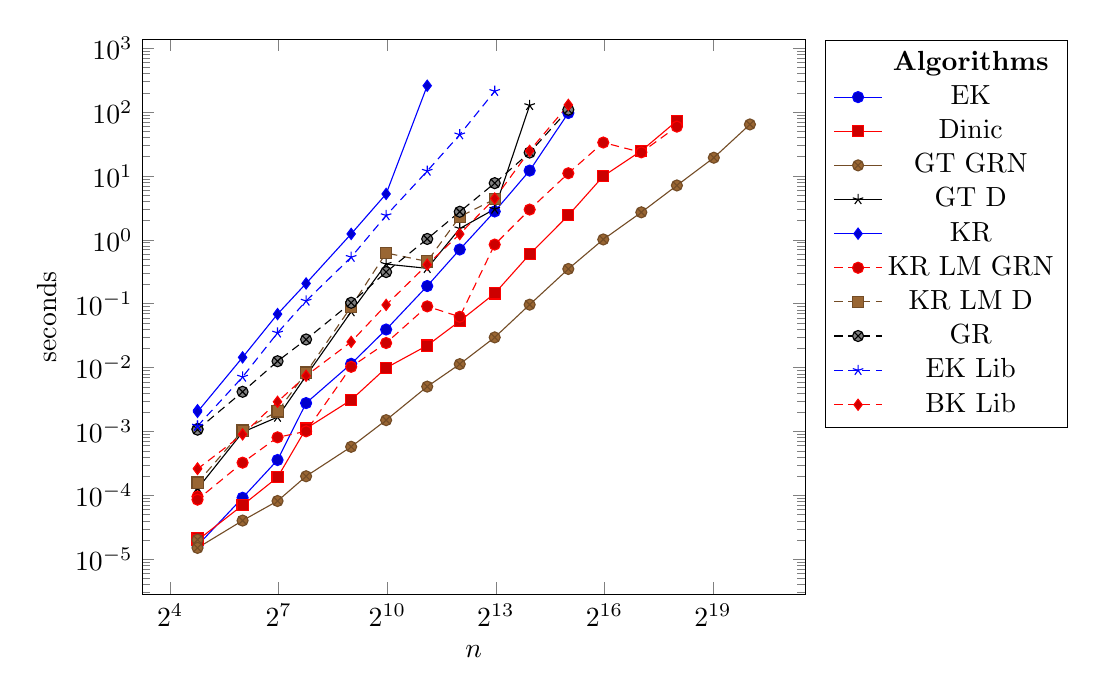
\begin{tikzpicture}
\begin{axis}[
    xlabel=$n$,ylabel=seconds,
    xmode=log,ymode=log,
    log basis x={2},
    legend style=
    {
        legend pos=outer north east
    },
    width=10cm
]
\addlegendimage{legend image code/.code=}
\legend{\textbf{Algorithms}, EK, Dinic, GT GRN, GT D, KR, KR LM GRN, KR LM D, GR, EK Lib, BK Lib}
\addplot table[x=n,y=value] {%EK
n value
27	1.83E-05
27	1.64353E-05
64	9.19488E-05
125	0.000358578
216	0.002789337
512	0.011478267
1000	0.039519567
2197	0.189271
4096	0.706506333
8000	2.78247
15625	12.12773333
32768	96.6569
};
\addplot table[x=n,y=value] {%Dinic
n value
27	2.16546E-05
27	1.98778E-05
64	7.04053E-05
125	0.000192226
216	0.001115157
512	0.003119373
1000	0.00991604
2197	0.0221898
4096	0.053542767
8000	0.144866667
15625	0.59337
32768	2.4171
64000	9.927513333
132651	24.71566667
262144	72.89203333
};
\addplot table[x=n,y=value] {%GT GRN
n value
27	2.03E-05
27	1.51027E-05
64	4.04221E-05
125	8.18436E-05
216	0.000199778
512	0.000577347
1000	0.001509167
2197	0.005050763
4096	0.0113486
8000	0.0297681
15625	0.096823533
32768	0.350279
64000	1.014996667
132651	2.6983
262144	7.101253333
531441	19.29156667
1061208	64.0214
};
\addplot table[x=n,y=value] {%GT D
n value
27	1.33E-04
27	0.000127152
64	0.000977459
125	0.00168207
216	0.007420783
512	0.0751745
1000	0.417246
2197	0.358329333
4096	1.503013333
8000	3.035766667
15625	127.1716667
};
\addplot table[x=n,y=value] {%KR
n value
27	2.16E-03
27	0.002033977
64	0.0144907
125	0.0688899
216	0.207899
512	1.23922
1000	5.23004
2197	258.178
};
\addplot table[x=n,y=value] {%KR LM GRN
n value
27	9.63E-05
27	8.59525E-05
64	0.000325931
125	0.000811551
216	0.001009107
512	0.010306333
1000	0.0242879
2197	0.090985567
4096	0.062492867
8000	0.84353
15625	2.978673333
32768	11.0194
64000	33.353
132651	23.40396667
262144	59.15526667
};
\addplot table[x=n,y=value] {%KR LM D
n value
27	1.61E-04
27	0.000158246
64	0.001037093
125	0.002061527
216	0.008381697
512	0.089949433
1000	0.622961333
2197	0.459367667
4096	2.298873333
8000	4.334706667
};
\addplot table[x=n,y=value] {%GR
n value
27	1.10E-03
27	0.00107007
64	0.004186893
125	0.0125998
216	0.027625867
512	0.103603333
1000	0.313361667
2197	1.03351
4096	2.753226667
8000	7.715346667
15625	23.232
32768	108.9246667
};
\addplot table[x=n,y=value] {%EK Lib
n value
27	0.001224103
27	0.001216997
64	0.007149513
125	0.0350155
216	0.110498333
512	0.535476
1000	2.40563
2197	11.93883333
4096	44.25053333
8000	211.9366667
};
\addplot table[x=n,y=value] {%BK Lib
n value
27	0.000264632
27	0.000259413
64	0.000902392
125	0.002922727
216	0.007462453
512	0.025325933
1000	0.095990433
2197	0.408633667
4096	1.230866667
8000	4.441643333
15625	24.72616667
32768	129.544
};
\end{axis}
\end{tikzpicture}
\caption{Best and worst results from the GenRmf square graphs}
\label{fig:GenRmf square_BW_ResultsAppendix}
\end{figure}


\begin{figure}[h]
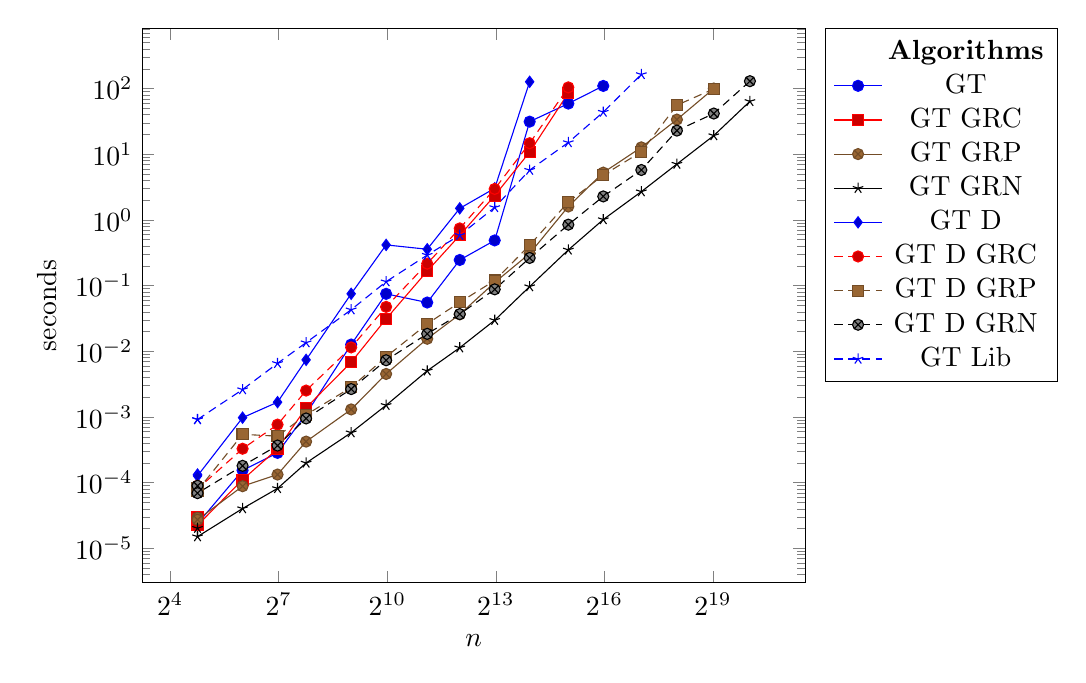
\begin{tikzpicture}
\begin{axis}[
    xlabel=$n$,ylabel=seconds,
    xmode=log,ymode=log,
    log basis x={2},
    legend style=
    {
        legend pos=outer north east
    },
    width=10cm
]
\addlegendimage{legend image code/.code=}
\legend{\textbf{Algorithms}, GT, GT GRC, GT GRP, GT GRN, GT D, GT D GRC, GT D GRP, GT D GRN, GT Lib}
\addplot table[x=n,y=value] {%GT
n value
27	2.54E-05
27	2.37646E-05
64	0.000153914
125	0.000284286
216	0.00111416
512	0.0126945
1000	0.075073033
2197	0.055363333
4096	0.245961333
8000	0.488409
15625	31.41703333
32768	59.17186667
64000	109.8606667
};
\addplot table[x=n,y=value] {%GT GRC
n value
27	3.03E-05
27	2.2432E-05
64	0.00011116
125	0.000326596
216	0.001382787
512	0.00682398
1000	0.031213833
2197	0.16648
4096	0.583621333
8000	2.351263333
15625	10.812
32768	85.61236667
};
\addplot table[x=n,y=value] {%GT GRP
n value
27	2.93E-05
27	2.73182E-05
64	8.83953E-05
125	0.000133037
216	0.000422432
512	0.00130516
1000	0.004525817
2197	0.0155378
4096	0.036563667
8000	0.111814333
15625	0.307891
32768	1.603586667
64000	5.25922
132651	12.75386667
262144	33.78733333
531441	100.2623333
};
\addplot table[x=n,y=value] {%GT GRN
n value
27	2.03E-05
27	1.51027E-05
64	4.04221E-05
125	8.18436E-05
216	0.000199778
512	0.000577347
1000	0.001509167
2197	0.005050763
4096	0.0113486
8000	0.0297681
15625	0.096823533
32768	0.350279
64000	1.014996667
132651	2.6983
262144	7.101253333
531441	19.29156667
1061208	64.0214
};
\addplot table[x=n,y=value] {%GT D
n value
27	1.33E-04
27	0.000127152
64	0.000977459
125	0.00168207
216	0.007420783
512	0.0751745
1000	0.417246
2197	0.358329333
4096	1.503013333
8000	3.035766667
15625	127.1716667
};
\addplot table[x=n,y=value] {%GT D GRC
n value
27	8.95E-05
27	8.04E-05
64	0.000328818
125	0.000766354
216	0.002527713
512	0.0114739
1000	0.0475249
2197	0.216508333
4096	0.744132
8000	2.9685
15625	14.74123333
32768	104.462
};
\addplot table[x=n,y=value] {%GT D GRP
n value
27	8.15E-05
27	7.59579E-05
64	0.000544588
125	0.000511051
216	0.001081957
512	0.002827437
1000	0.008248543
2197	0.026213167
4096	0.055797467
8000	0.119685667
15625	0.412618667
32768	1.87621
64000	4.814616667
132651	10.91256667
262144	55.88503333
531441	99.03183333
};
\addplot table[x=n,y=value] {%GT D GRN
n value
27	8.98E-05
27	0.000069295
64	0.000180789
125	0.000367908
216	0.000950806
512	0.00266219
1000	0.00731351
2197	0.018466767
4096	0.036885933
8000	0.0878232
15625	0.264105667
32768	0.848473667
64000	2.283013333
132651	5.76648
262144	22.9456
531441	41.73593333
1061208	129.805
};
\addplot table[x=n,y=value] {%GT Lib
n value
27	0.000922159
27	0.000915052
64	0.002620227
125	0.006562393
216	0.013568533
512	0.043020667
1000	0.114954
2197	0.291912667
4096	0.586437667
8000	1.553093333
15625	5.743833333
32768	15.12613333
64000	43.95683333
132651	164.3336667
};
\end{axis}
\end{tikzpicture}
\caption{Goldberg and Tarjan results from the GenRmf square graphs}
\label{fig:GenRmf square_GT_ResultsAppendix}
\end{figure}


\begin{figure}[h]
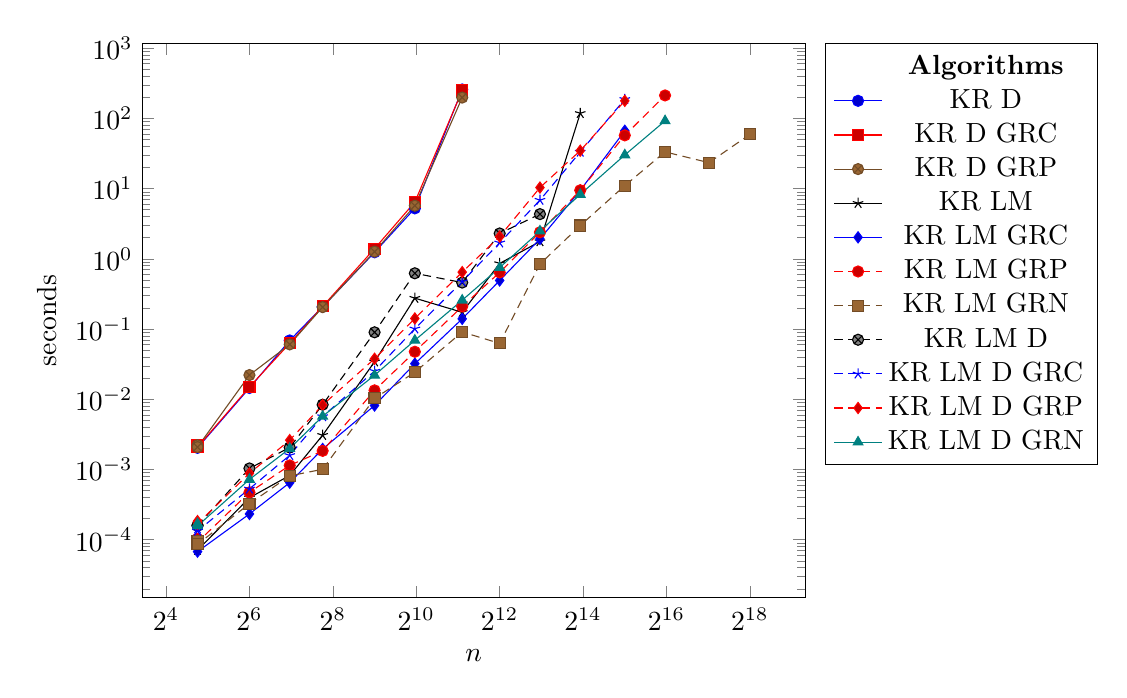
\begin{tikzpicture}
\begin{axis}[
    xlabel=$n$,ylabel=seconds,
    xmode=log,ymode=log,
    log basis x={2},
    legend style=
    {
        legend pos=outer north east
    },
    width=10cm
]
\addlegendimage{legend image code/.code=}
\legend{\textbf{Algorithms}, KR D, KR D GRC, KR D GRP, KR LM, KR LM GRC, KR LM GRP, KR LM GRN, KR LM D, KR LM D GRC, KR LM D GRP, KR LM D GRN}
\addplot table[x=n,y=value] {%KR
n value
27	2.16E-03
27	0.002033977
64	0.0144907
125	0.0688899
216	0.207899
512	1.23922
1000	5.23004
2197	258.178
};
\addplot table[x=n,y=value] {%KR GRC
n value
27	2.23E-03
27	0.00208284
64	0.014971033
125	0.062672033
216	0.210346
512	1.397736667
1000	6.43309
2197	249.9376667
};
\addplot table[x=n,y=value] {%KR GRP
n value
27	2.22E-03
27	0.002085847
64	0.022137767
125	0.060497533
216	0.205200667
512	1.26544
1000	5.717356667
2197	198.016
};
\addplot table[x=n,y=value] {%KR LM
n value
27	7.78E-05
27	7.11828E-05
64	0.000396225
125	0.000823766
216	0.003079187
512	0.034277133
1000	0.275727667
2197	0.173293667
4096	0.859855333
8000	1.765033333
15625	118.149
};
\addplot table[x=n,y=value] {%KR LM GRC
n value
27	7.58E-05
27	6.77403E-05
64	0.000232871
125	0.000650307
216	0.00196269
512	0.008164487
1000	0.0320805
2197	0.139880333
4096	0.492149333
8000	1.92034
15625	9.41052
32768	66.65046667
};
\addplot table[x=n,y=value] {%KR LM GRP
n value
27	1.03E-04
27	9.21711E-05
64	0.000473294
125	0.001145363
216	0.00184309
512	0.013407133
1000	0.047549267
2197	0.209707
4096	0.641041333
8000	2.392316667
15625	9.472133333
32768	57.29816667
64000	212.2696667
};
\addplot table[x=n,y=value] {%KR LM GRN
n value
27	9.63E-05
27	8.59525E-05
64	0.000325931
125	0.000811551
216	0.001009107
512	0.010306333
1000	0.0242879
2197	0.090985567
4096	0.062492867
8000	0.84353
15625	2.978673333
32768	11.0194
64000	33.353
132651	23.40396667
262144	59.15526667
};
\addplot table[x=n,y=value] {%KR LM D
n value
27	1.61E-04
27	0.000158246
64	0.001037093
125	0.002061527
216	0.008381697
512	0.089949433
1000	0.622961333
2197	0.459367667
4096	2.298873333
8000	4.334706667
};
\addplot table[x=n,y=value] {%KR LM D GRC
n value
27	1.43E-04
27	0.000133593
64	0.000530595
125	0.001592453
216	0.005694627
512	0.025246367
1000	0.100972333
2197	0.473784333
4096	1.692813333
8000	6.861693333
15625	33.215
32768	187.0353333
};
\addplot table[x=n,y=value] {%KR LM D GRP
n value
27	1.84E-04
27	0.000169795
64	0.000882734
125	0.00262177
216	0.008297853
512	0.037802967
1000	0.141620333
2197	0.646652
4096	2.074956667
8000	10.3482
15625	34.67336667
32768	177.815
};
\addplot[mark=triangle*, teal] table[x=n,y=value] {%KR LM D GRN
n value
27	1.70E-04
27	0.000157357
64	0.0007226
125	0.001988787
216	0.005735383
512	0.022002833
1000	0.0692056
2197	0.257478
4096	0.750494333
8000	2.48334
15625	8.26
32768	30.14693333
64000	92.17513333
};
\end{axis}
\end{tikzpicture}
\caption{King and Rao results from the GenRmf square graphs}
\label{fig:GenRmf square_KR_Results}
\end{figure}

%-----------------------------------------------------------------------------------------------------------
\clearpage


\subsection{Results from Wash long graphs}
\begin{figure}[h]
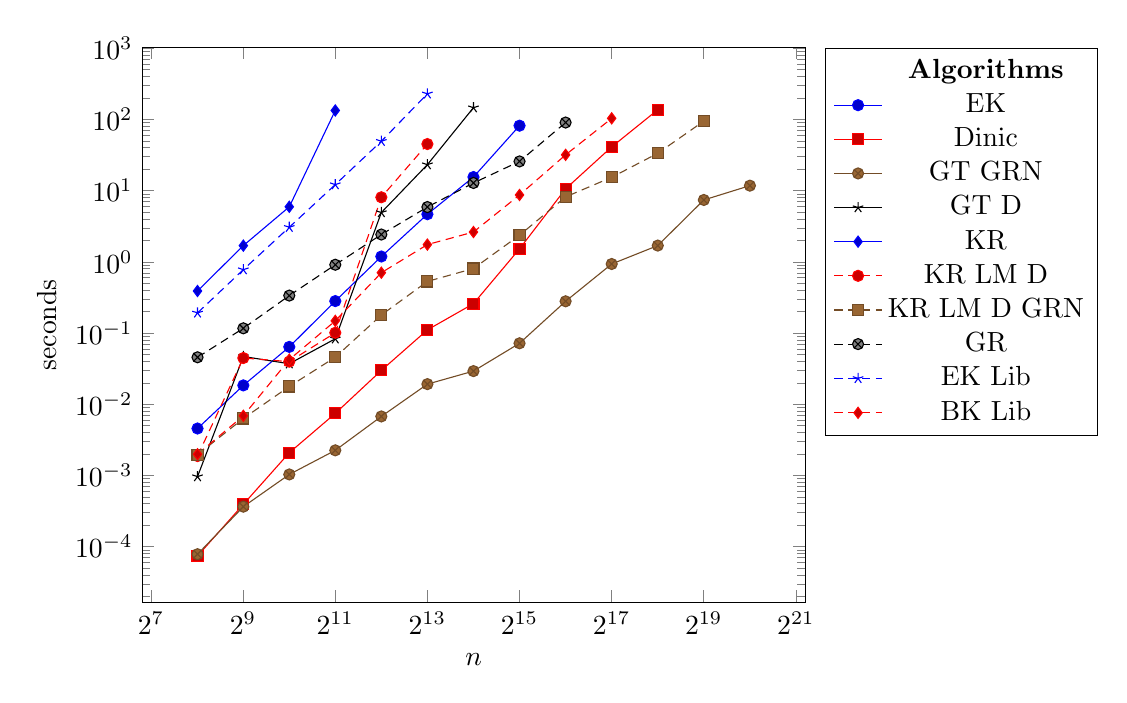
\begin{tikzpicture}
\begin{axis}[
    xlabel=$n$,ylabel=seconds,
    xmode=log,ymode=log,
    log basis x={2},
    legend style=
    {
        legend pos=outer north east
    },
    width=10cm
]
\addlegendimage{legend image code/.code=}
\legend{\textbf{Algorithms}, EK, Dinic, GT GRN, GT D, KR, KR LM D, KR LM D GRN, GR, EK Lib, BK Lib}
\addplot table[x=n,y=value] {%EK
n value
258	0.00455813
514	0.018388
1026	0.063829267
2050	0.280650667
4098	1.186396667
8194	4.660366667
16386	15.4853
32770	81.58816667
};
\addplot table[x=n,y=value] {%Dinic
n value
258	7.39589E-05
514	0.000392448
1026	0.00208284
2050	0.007431643
4098	0.0298423
8194	0.110588
16386	0.258280667
32770	1.520013333
65538	10.58663333
131074	41.0456
262146	136.5323333
};
\addplot table[x=n,y=value] {%GT GRN
n value
258	0.00007829
514	0.000364021
1026	0.00103243
2050	0.002250977
4098	0.00673583
8194	0.0191461
16386	0.029171
32770	0.071709467
65538	0.278762667
131074	0.931172
262146	1.689216667
524290	7.384293333
1048576	11.7299
};
\addplot table[x=n,y=value] {%GT D
n value
258	0.000963133
514	0.046797767
1026	0.037027933
2050	0.082945567
4098	4.91926
8194	23.14326667
16386	145.951
};
\addplot table[x=n,y=value] {%KR
n value
258	0.388986
514	1.687986667
1026	5.91655
2050	133.461
};
\addplot table[x=n,y=value] {%KR LM D
n value
258	0.001871523
514	0.044522067
1026	0.0396492
2050	0.100842
4098	8.054103333
8194	45.0224
};
\addplot table[x=n,y=value] {%KR LM D GRN
n value
258	0.001956473
514	0.006307733
1026	0.0177545
2050	0.045698067
4098	0.178866333
8194	0.530067
16386	0.803962667
32770	2.36107
65538	8.150896667
131074	15.36236667
262146	33.3926
524290	94.52643333
};
\addplot table[x=n,y=value] {%GR
n value
258	0.0455862
514	0.116387
1026	0.335383333
2050	0.909223667
4098	2.416166667
8194	5.87323
16386	12.79106667
32770	25.68216667
65538	90.29623333
};
\addplot table[x=n,y=value] {%EK Lib
n value
258	0.191596667
514	0.776001
1026	3.056936667
2050	12.1327
4098	49.3162
8194	228.5943333
};
\addplot table[x=n,y=value] {%BK Lib
n value
258	0.001984353
514	0.006870553
1026	0.0423145
2050	0.147986667
4098	0.702769333
8194	1.744473333
16386	2.61717
32770	8.679073333
65538	31.74643333
131074	103.3123333
};
\end{axis}
\end{tikzpicture}
\caption{Best and worst results from the Wash long graphs}
\label{fig:Wash long_BW_Results}
\end{figure}


\begin{figure}[h]
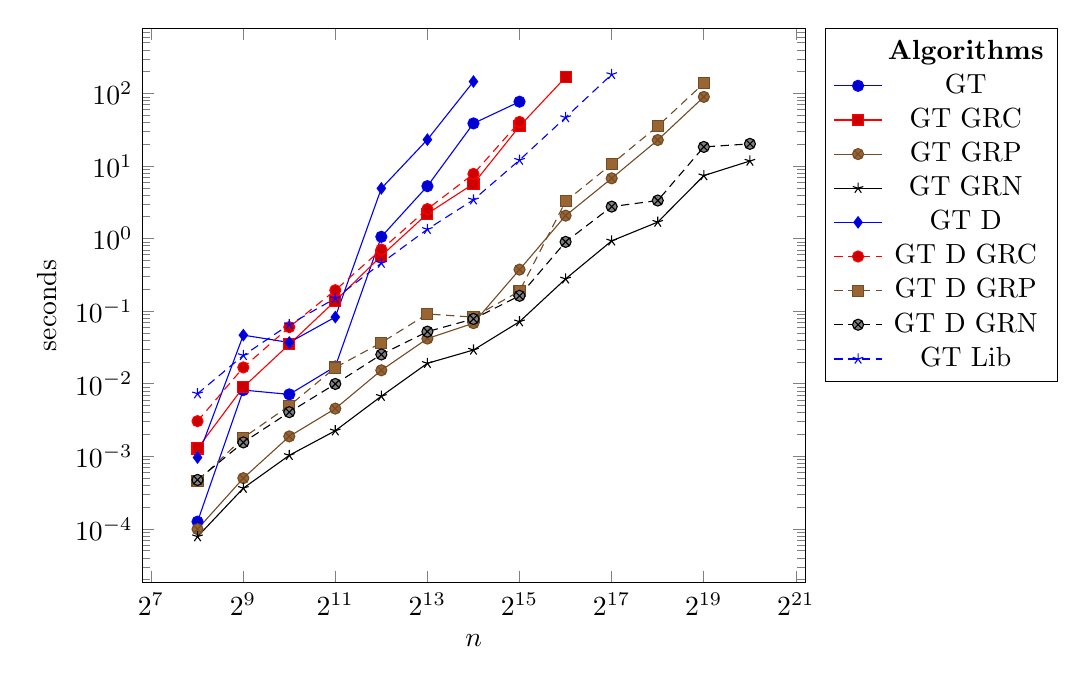
\begin{tikzpicture}
\begin{axis}[
    xlabel=$n$,ylabel=seconds,
    xmode=log,ymode=log,
    log basis x={2},
    legend style=
    {
        legend pos=outer north east
    },
    width=10cm
]
\addlegendimage{legend image code/.code=}
\legend{\textbf{Algorithms}, GT, GT GRC, GT GRP, GT GRN, GT D, GT D GRC, GT D GRP, GT D GRN, GT Lib}
\addplot table[x=n,y=value] {%GT
n value
258	0.000125819
514	0.008185667
1026	0.007138363
2050	0.017273933
4098	1.059973333
8194	5.279913333
16386	38.7052
32770	77.06073333
};
\addplot table[x=n,y=value] {%GT GRC
n value
258	0.001285393
514	0.008987553
1026	0.034958967
2050	0.138807
4098	0.579380667
8194	2.207283333
16386	5.693513333
32770	35.35053333
65538	167.6426667
};
\addplot table[x=n,y=value] {%GT GRP
n value
258	9.92782E-05
514	0.000500499
1026	0.00188184
2050	0.00454514
4098	0.015331
8194	0.041919
16386	0.068337667
32770	0.374196333
65538	2.072736667
131074	6.770743333
262146	22.8228
524290	89.71463333
};
\addplot table[x=n,y=value] {%GT GRN
n value
258	0.00007829
514	0.000364021
1026	0.00103243
2050	0.002250977
4098	0.00673583
8194	0.0191461
16386	0.029171
32770	0.071709467
65538	0.278762667
131074	0.931172
262146	1.689216667
524290	7.384293333
1048576	11.7299
};
\addplot table[x=n,y=value] {%GT D
n value
258	0.000963133
514	0.046797767
1026	0.037027933
2050	0.082945567
4098	4.91926
8194	23.14326667
16386	145.951
};
\addplot table[x=n,y=value] {%GT D GRC
n value
258	0.0030522
514	0.0168027
1026	0.0603235
2050	0.194416667
4098	0.707329333
8194	2.552136667
16386	7.796243333
32770	40.53683333
};
\addplot table[x=n,y=value] {%GT D GRP
n value
258	0.000453305
514	0.001807667
1026	0.00497547
2050	0.016712433
4098	0.036814533
8194	0.091586867
16386	0.082781533
32770	0.188612667
65538	3.26371
131074	10.66083333
262146	35.4517
524290	138.2766667
};
\addplot table[x=n,y=value] {%GT D GRN
n value
258	0.000472849
514	0.00155514
1026	0.00405964
2050	0.00993795
4098	0.025338533
8194	0.052303033
16386	0.0782536
32770	0.162790667
65538	0.901931333
131074	2.760933333
262146	3.348056667
524290	18.34756667
1048576	20.21003333
};
\addplot table[x=n,y=value] {%GT Lib
n value
258	0.007290433
514	0.024574033
1026	0.065415467
2050	0.150266333
4098	0.459179333
8194	1.343486667
16386	3.42729
32770	12.08016667
65538	46.69996667
131074	182.9003333
};
\end{axis}
\end{tikzpicture}
\caption{Goldberg and Tarjan results from the Wash long graphs}
\label{fig:Wash long_GT_Results}
\end{figure}


\begin{figure}[h]
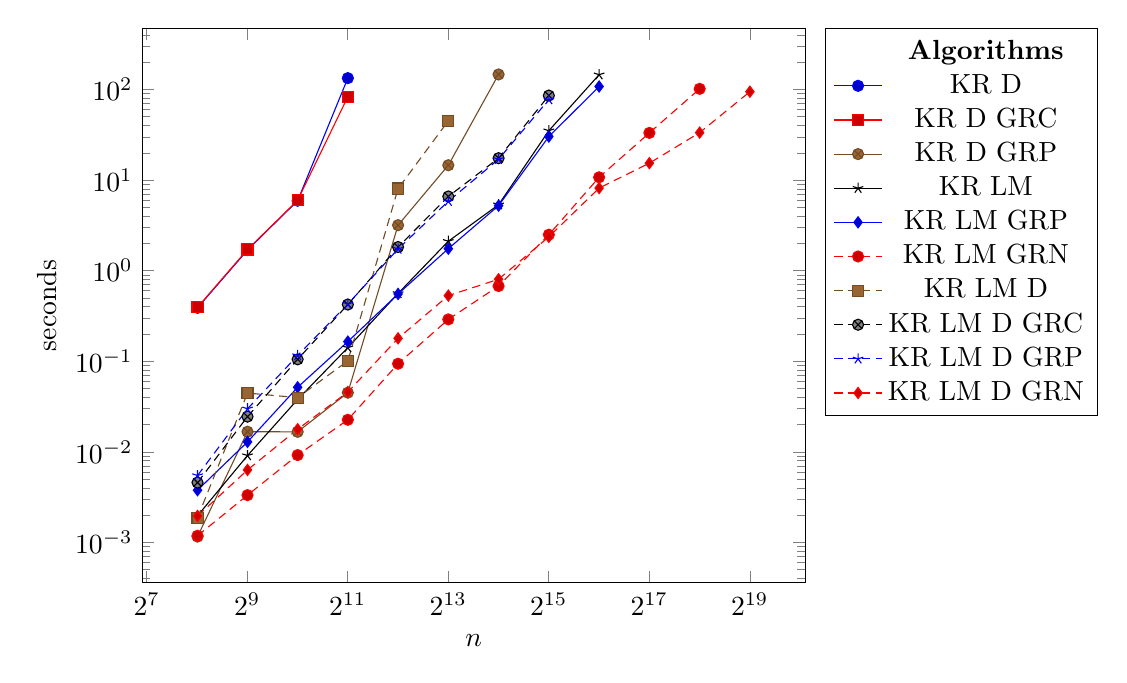
\begin{tikzpicture}
\begin{axis}[
    xlabel=$n$,ylabel=seconds,
    xmode=log,ymode=log,
    log basis x={2},
    legend style=
    {
        legend pos=outer north east
    },
    width=10cm
]
\addlegendimage{legend image code/.code=}
\legend{\textbf{Algorithms}, KR D, KR D GRC, KR D GRP, KR LM, KR LM GRP, KR LM GRN, KR LM D, KR LM D GRC, KR LM D GRP, KR LM D GRN}
\addplot table[x=n,y=value] {%KR
n value
258	0.388986
514	1.687986667
1026	5.91655
2050	133.461
};
\addplot table[x=n,y=value] {%KR GRP
n value
258	0.394335667
514	1.712723333
1026	5.980416667
2050	83.11296667
};
\addplot table[x=n,y=value] {%KR LM
n value
258	0.001158027
514	0.016664333
1026	0.0166107
2050	0.044975967
4098	3.17705
8194	14.57306667
16386	146.5643333
};
\addplot table[x=n,y=value] {%KR LM GRC
n value
258	0.0019678
514	0.00909097
1026	0.037847933
2050	0.141140667
4098	0.560116
8194	2.111113333
16386	5.345923333
32770	35.08333333
65538	145.6033333
};
\addplot table[x=n,y=value] {%KR LM GRP
n value
258	0.003771133
514	0.0128673
1026	0.051574
2050	0.164608333
4098	0.552708
8194	1.747106667
16386	5.22136
32770	30.23373333
65538	107.821
};
\addplot table[x=n,y=value] {%KR LM GRN
n value
258	0.001184233
514	0.003323717
1026	0.00919758
2050	0.022584967
4098	0.093840167
8194	0.289705333
16386	0.67618
32770	2.49438
65538	10.7308
131074	33.17436667
262146	101.676
};
\addplot table[x=n,y=value] {%KR LM D
n value
258	0.001871523
514	0.044522067
1026	0.0396492
2050	0.100842
4098	8.054103333
8194	45.0224
};
\addplot table[x=n,y=value] {%KR LM D GRC
n value
258	0.004577133
514	0.024459433
1026	0.104925
2050	0.422261
4098	1.82286
8194	6.58966
16386	17.44673333
32770	85.69343333
};
\addplot table[x=n,y=value] {%KR LM D GRP
n value
258	0.005469973
514	0.029860167
1026	0.115612667
2050	0.42751
4098	1.734793333
8194	5.83833
16386	16.96373333
32770	77.27503333
};
\addplot table[x=n,y=value] {%KR LM D GRN
n value
258	0.001956473
514	0.006307733
1026	0.0177545
2050	0.045698067
4098	0.178866333
8194	0.530067
16386	0.803962667
32770	2.36107
65538	8.150896667
131074	15.36236667
262146	33.3926
524290	94.52643333
};
\end{axis}
\end{tikzpicture}
\caption{King and Rao results from the Wash long graphs}
\label{fig:Wash long_KR_Results}
\end{figure}

%-----------------------------------------------------------------------------------------------------------
\clearpage


\subsection{Results from Wash wide graphs}
\begin{figure}[h]
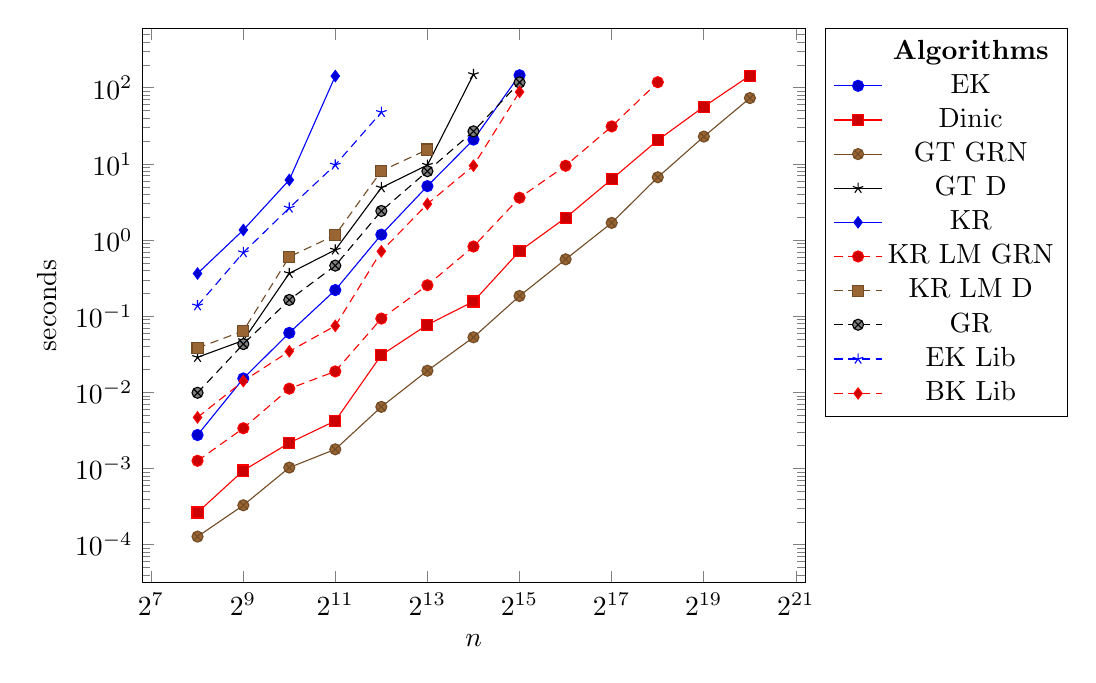
\begin{tikzpicture}
\begin{axis}[
    xlabel=$n$,ylabel=seconds,
    xmode=log,ymode=log,
    log basis x={2},
    legend style=
    {
        legend pos=outer north east
    },
    width=10cm
]
\addlegendimage{legend image code/.code=}
\legend{\textbf{Algorithms}, EK, Dinic, GT GRN, GT D, KR, KR LM GRN, KR LM D, GR, EK Lib, BK Lib}
\addplot table[x=n,y=value] {%EK
n value
258	0.00275391
514	0.0152435
1026	0.060453233
2050	0.220815
4098	1.178703333
8194	5.108153333
16386	20.86096667
32770	145.9943333
};
\addplot table[x=n,y=value] {%Dinic
n value
258	0.000264853
514	0.000941476
1026	0.002168793
2050	0.00422976
4098	0.030909467
8194	0.0773594
16386	0.156071667
32770	0.715507333
65538	1.959956667
131074	6.289176667
262146	20.50246667
524290	56.4742
1048578	144.392
};
\addplot table[x=n,y=value] {%GT GRN
n value
258	0.000127707
514	0.000329373
1026	0.001029652
2050	0.001789457
4098	0.00645676
8194	0.0192589
16386	0.052897167
32770	0.184429667
65538	0.559192
131074	1.680873333
262146	6.679286667
524290	22.85353333
1048578	73.2423
};
\addplot table[x=n,y=value] {%GT D
n value
258	0.028931
514	0.0480383
1026	0.366069
2050	0.743220667
4098	4.87707
8194	9.65479
16386	149.6193333
};
\addplot table[x=n,y=value] {%KR
n value
258	0.363904333
514	1.35767
1026	6.165536667
2050	142.452
};
\addplot table[x=n,y=value] {%KR LM GRN
n value
258	0.00126419
514	0.003382793
1026	0.011198767
2050	0.018873433
4098	0.0931617
8194	0.255151667
16386	0.822616667
32770	3.595813333
65538	9.45794
131074	31.09106667
262146	118.3703333
};
\addplot table[x=n,y=value] {%KR LM D
n value
258	0.038245967
514	0.064131167
1026	0.602363
2050	1.16391
4098	8.07734
8194	15.42616667
};
\addplot table[x=n,y=value] {%GR
n value
258	0.00988439
514	0.043069933
1026	0.163758333
2050	0.462004333
4098	2.41123
8194	8.02773
16386	26.78126667
32770	117.4263333
};
\addplot table[x=n,y=value] {%EK Lib
n value
258	0.137420667
514	0.686362333
1026	2.640513333
2050	9.708146667
4098	47.70486667
};
\addplot table[x=n,y=value] {%BK Lib
n value
258	0.00469564
514	0.014075633
1026	0.0346164
2050	0.074734567
4098	0.711892
8194	2.98372
16386	9.469473333
32770	88.19736667
};
\end{axis}
\end{tikzpicture}
\caption{Best and worst results from the Wash wide graphs}
\label{fig:Wash wide_BW_Results}
\end{figure}


\begin{figure}[h]
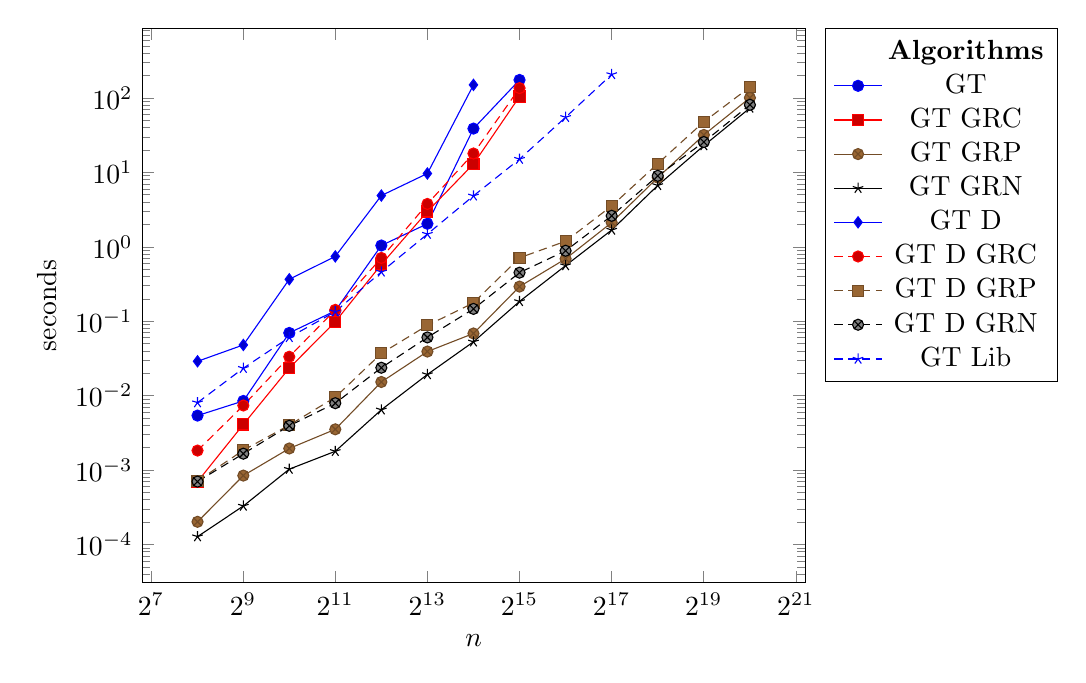
\begin{tikzpicture}
\begin{axis}[
    xlabel=$n$,ylabel=seconds,
    xmode=log,ymode=log,
    log basis x={2},
    legend style=
    {
        legend pos=outer north east
    },
    width=10cm
]
\addlegendimage{legend image code/.code=}
\legend{\textbf{Algorithms}, GT, GT GRC, GT GRP, GT GRN, GT D, GT D GRC, GT D GRP, GT D GRN, GT Lib}
\addplot table[x=n,y=value] {%GT
n value
258	0.005397887
514	0.00849272
1026	0.069627133
2050	0.137981667
4098	1.041136667
8194	2.039763333
16386	38.72533333
32770	174.4586667
};
\addplot table[x=n,y=value] {%GT GRC
n value
258	0.000700388
514	0.004106717
1026	0.0234676
2050	0.0985133
4098	0.578804
8194	2.978286667
16386	12.9586
32770	104.409
};
\addplot table[x=n,y=value] {%GT GRP
n value
258	0.000201999
514	0.000843642
1026	0.001951807
2050	0.00353048
4098	0.015270067
8194	0.0391442
16386	0.068477133
32770	0.291984
65538	0.689515
131074	2.116356667
262146	8.503033333
524290	31.83243333
1048578	100.3662333
};
\addplot table[x=n,y=value] {%GT GRN
n value
258	0.000127707
514	0.000329373
1026	0.001029652
2050	0.001789457
4098	0.00645676
8194	0.0192589
16386	0.052897167
32770	0.184429667
65538	0.559192
131074	1.680873333
262146	6.679286667
524290	22.85353333
1048578	73.2423
};
\addplot table[x=n,y=value] {%GT D
n value
258	0.028931
514	0.0480383
1026	0.366069
2050	0.743220667
4098	4.87707
8194	9.65479
16386	149.6193333
};
\addplot table[x=n,y=value] {%GT D GRC
n value
258	0.00182921
514	0.007377473
1026	0.0333401
2050	0.142173667
4098	0.708439333
8194	3.76566
16386	17.92476667
32770	135.5356667
};
\addplot table[x=n,y=value] {%GT D GRP
n value
258	0.000714938
514	0.001848203
1026	0.004024107
2050	0.00951629
4098	0.037023733
8194	0.087905367
16386	0.176312
32770	0.711375
65538	1.187876667
131074	3.542926667
262146	13.07743333
524290	47.78543333
1048578	140.107
};
\addplot table[x=n,y=value] {%GT D GRN
n value
258	0.000700724
514	0.001661527
1026	0.003936377
2050	0.007919837
4098	0.023725
8194	0.060609267
16386	0.146432
32770	0.449296
65538	0.884841667
131074	2.60916
262146	8.989773333
524290	25.54076667
1048578	80.799
};
\addplot table[x=n,y=value] {%GT Lib
n value
258	0.00805746
514	0.023360733
1026	0.060663733
2050	0.134216
4098	0.459610333
8194	1.481406667
16386	4.83742
32770	15.06266667
65538	54.98906667
131074	206.772
};
\end{axis}
\end{tikzpicture}
\caption{Goldberg and Tarjan results from the Wash wide graphs}
\label{fig:Wash wide_GT_Results}
\end{figure}


\begin{figure}[h]
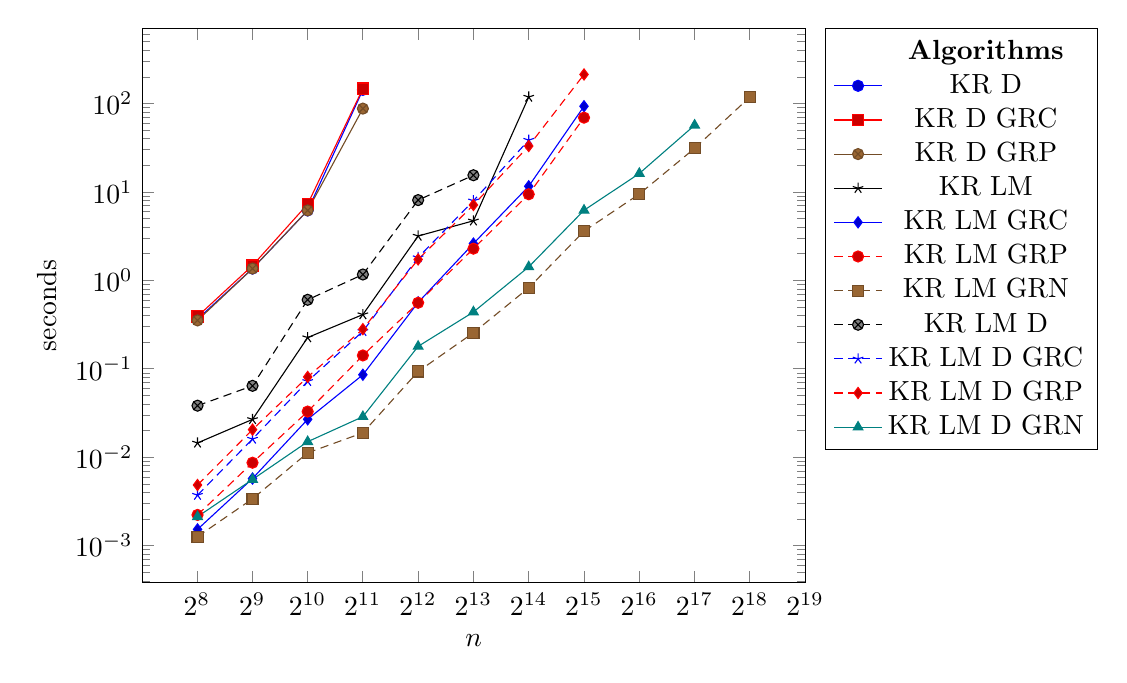
\begin{tikzpicture}
\begin{axis}[
    xlabel=$n$,ylabel=seconds,
    xmode=log,ymode=log,
    log basis x={2},
    legend style=
    {
        legend pos=outer north east
    },
    width=10cm
]
\addlegendimage{legend image code/.code=}
\legend{\textbf{Algorithms}, KR D, KR D GRC, KR D GRP, KR LM, KR LM GRC, KR LM GRP, KR LM GRN, KR LM D, KR LM D GRC, KR LM D GRP, KR LM D GRN}
\addplot table[x=n,y=value] {%KR
n value
258	0.363904333
514	1.35767
1026	6.165536667
2050	142.452
};
\addplot table[x=n,y=value] {%KR GRC
n value
258	0.390611333
514	1.4708
1026	7.269586667
2050	147.5433333
};
\addplot table[x=n,y=value] {%KR GRP
n value
258	0.352055333
514	1.358303333
1026	6.17634
2050	87.4755
};
\addplot table[x=n,y=value] {%KR LM
n value
258	0.014494433
514	0.0267644
1026	0.225451667
2050	0.410102
4098	3.170193333
8194	4.711013333
16386	118.326
};
\addplot table[x=n,y=value] {%KR LM GRC
n value
258	0.001526377
514	0.005739157
1026	0.026819933
2050	0.085569067
4098	0.562867
8194	2.602023333
16386	11.57923333
32770	92.96356667
};
\addplot table[x=n,y=value] {%KR LM GRP
n value
258	0.00222466
514	0.008658543
1026	0.0328203
2050	0.141411
4098	0.557627
8194	2.280763333
16386	9.398566667
32770	69.1255
};
\addplot table[x=n,y=value] {%KR LM GRN
n value
258	0.00126419
514	0.003382793
1026	0.011198767
2050	0.018873433
4098	0.0931617
8194	0.255151667
16386	0.822616667
32770	3.595813333
65538	9.45794
131074	31.09106667
262146	118.3703333
};
\addplot table[x=n,y=value] {%KR LM D
n value
258	0.038245967
514	0.064131167
1026	0.602363
2050	1.16391
4098	8.07734
8194	15.42616667
};
\addplot table[x=n,y=value] {%KR LM D GRC
n value
258	0.003725053
514	0.016062567
1026	0.0721805
2050	0.265253667
4098	1.81085
8194	7.93862
16386	38.531
};
\addplot table[x=n,y=value] {%KR LM D GRP
n value
258	0.00484776
514	0.020500433
1026	0.0808727
2050	0.280267333
4098	1.72412
8194	7.104583333
16386	32.9985
32770	212.8473333
};
\addplot[mark=triangle*, teal] table[x=n,y=value] {%KR LM D GRN
n value
258	0.002122937
514	0.005603013
1026	0.014965867
2050	0.028723433
4098	0.179154667
8194	0.438172
16386	1.418813333
32770	6.193153333
65538	16.14906667
131074	56.7592
};
\end{axis}
\end{tikzpicture}
\caption{King and Rao results from the Wash wide graphs}
\label{fig:Wash wide_KR_Results}
\end{figure}


%-----------------------------------------------------------------------------------------------------------
\clearpage


\subsection{Results from Computer Vision graphs}
\begin{figure}[h]
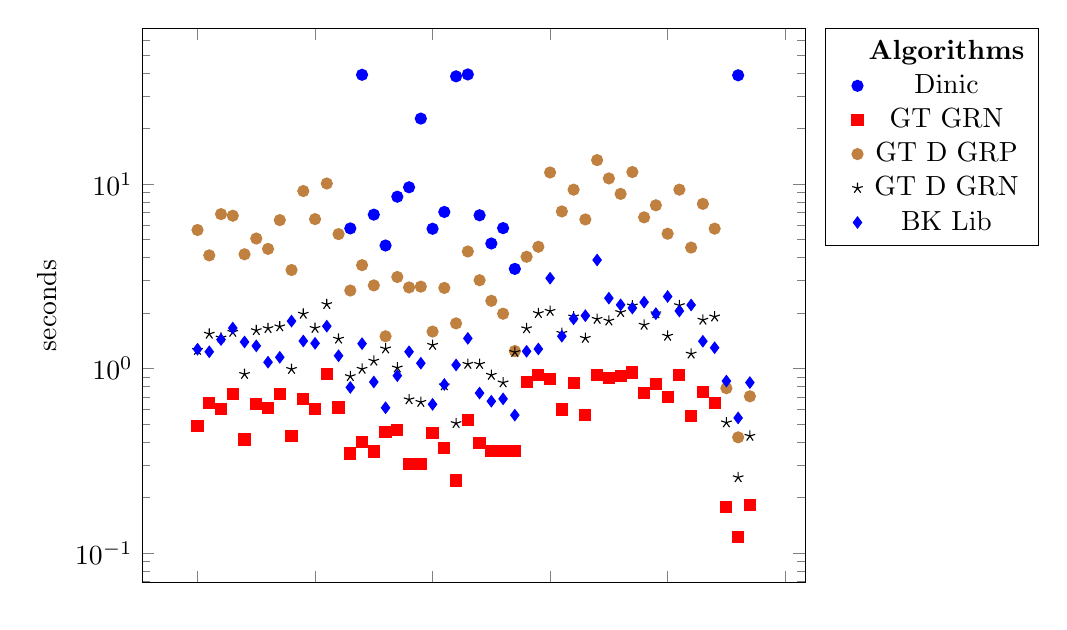
\begin{tikzpicture}
\begin{axis}[
    ylabel=seconds,ymode=log,
	symbolic x coords={BVZ-sawtooth04,BVZ-sawtooth06,BVZ-sawtooth07,BVZ-sawtooth08,BVZ-sawtooth09,BVZ-sawtooth10,BVZ-sawtooth11,BVZ-sawtooth12,BVZ-sawtooth13,BVZ-sawtooth14,BVZ-sawtooth15,BVZ-sawtooth16,BVZ-sawtooth18,BVZ-tsukuba00,BVZ-tsukuba01,BVZ-tsukuba02,BVZ-tsukuba03,BVZ-tsukuba04,BVZ-tsukuba05,BVZ-tsukuba6,BVZ-tsukuba7,BVZ-tsukuba8,BVZ-tsukuba9,BVZ-tsukuba10,BVZ-tsukuba11,BVZ-tsukuba12,BVZ-tsukuba14,BVZ-tsukuba15,BVZ-venus01,BVZ-venus02,BVZ-venus03,BVZ-venus04,BVZ-venus05,BVZ-venus06,BVZ-venus07,BVZ-venus08,BVZ-venus09,BVZ-venus10,BVZ-venus11,BVZ-venus12,BVZ-venus13,BVZ-venus14,BVZ-venus15,BVZ-venus16,BVZ-venus17,KZ2-sawtooth17,KZ2-tsukuba13,KZ2-venus19},
	xticklabels={,,},
    legend style=
    {
        legend pos=outer north east
    },
    width=10cm
]
\addlegendimage{legend image code/.code=}
\legend{\textbf{Algorithms}, Dinic, GT GRN, GT D GRP, GT D GRN, BK Lib}
\addplot[only marks, blue, mark=*] table[x=n,y=value] {%Dinic
n value
BVZ-tsukuba00	5.750836667
BVZ-tsukuba01	39.14823333
BVZ-tsukuba02	6.83006
BVZ-tsukuba03	4.645143333
BVZ-tsukuba04	8.541403333
BVZ-tsukuba05	9.609163333
BVZ-tsukuba10	39.3178
BVZ-tsukuba11	6.7765
BVZ-tsukuba12	4.763366667
BVZ-tsukuba14	5.771553333
BVZ-tsukuba15	3.468896667
BVZ-tsukuba6	22.6535
BVZ-tsukuba7	5.724696667
BVZ-tsukuba8	7.061796667
BVZ-tsukuba9	38.3952
KZ2-tsukuba13	38.90546667
};
\addplot[only marks, red, mark=square*] table[x=n,y=value] {%GT GRN
n value
BVZ-sawtooth04	0.489767333
BVZ-sawtooth06	0.650722667
BVZ-sawtooth07	0.602036667
BVZ-sawtooth08	0.728916
BVZ-sawtooth09	0.412417333
BVZ-sawtooth10	0.642597
BVZ-sawtooth11	0.610116
BVZ-sawtooth12	0.731337
BVZ-sawtooth13	0.429253333
BVZ-sawtooth14	0.683659333
BVZ-sawtooth15	0.604143
BVZ-sawtooth16	0.933819
BVZ-sawtooth18	0.614827667
BVZ-tsukuba00	0.346019
BVZ-tsukuba01	0.39826
BVZ-tsukuba02	0.355036667
BVZ-tsukuba03	0.452382667
BVZ-tsukuba04	0.462989667
BVZ-tsukuba05	0.302774
BVZ-tsukuba10	0.523340333
BVZ-tsukuba11	0.394437667
BVZ-tsukuba12	0.357265333
BVZ-tsukuba14	0.356760667
BVZ-tsukuba15	0.358245
BVZ-tsukuba6	0.30229
BVZ-tsukuba7	0.447588333
BVZ-tsukuba8	0.371264
BVZ-tsukuba9	0.247241333
BVZ-venus01	0.844272667
BVZ-venus02	0.918598
BVZ-venus03	0.873629667
BVZ-venus04	0.599272
BVZ-venus05	0.836556333
BVZ-venus06	0.559744667
BVZ-venus07	0.920171667
BVZ-venus08	0.885694
BVZ-venus09	0.912648
BVZ-venus10	0.951088333
BVZ-venus11	0.740437333
BVZ-venus12	0.821746
BVZ-venus13	0.702746333
BVZ-venus14	0.926211
BVZ-venus15	0.550986667
BVZ-venus16	0.742330333
BVZ-venus17	0.649391333
KZ2-sawtooth17	0.177902
KZ2-tsukuba13	0.12262
KZ2-venus19	0.181196667
};
\addplot[only marks, brown, mark=oplus*] table[x=n,y=value] {%GT D GRP
n value
BVZ-sawtooth04	5.637843333
BVZ-sawtooth06	4.106903333
BVZ-sawtooth07	6.87372
BVZ-sawtooth08	6.738953333
BVZ-sawtooth09	4.163056667
BVZ-sawtooth10	5.067443333
BVZ-sawtooth11	4.45305
BVZ-sawtooth12	6.378663333
BVZ-sawtooth13	3.42055
BVZ-sawtooth14	9.17015
BVZ-sawtooth15	6.45878
BVZ-sawtooth16	10.07306667
BVZ-sawtooth18	5.355506667
BVZ-tsukuba00	2.647463333
BVZ-tsukuba01	3.635553333
BVZ-tsukuba02	2.823506667
BVZ-tsukuba03	1.495733333
BVZ-tsukuba04	3.1349
BVZ-tsukuba05	2.75291
BVZ-tsukuba10	4.310993333
BVZ-tsukuba11	3.01142
BVZ-tsukuba12	2.328253333
BVZ-tsukuba14	1.98249
BVZ-tsukuba15	1.243746667
BVZ-tsukuba6	2.779606667
BVZ-tsukuba7	1.58586
BVZ-tsukuba8	2.73537
BVZ-tsukuba9	1.757243333
BVZ-venus01	4.034523333
BVZ-venus02	4.57276
BVZ-venus03	11.55953333
BVZ-venus04	7.10882
BVZ-venus05	9.328716667
BVZ-venus06	6.432303333
BVZ-venus07	13.49126667
BVZ-venus08	10.73153333
BVZ-venus09	8.848846667
BVZ-venus10	11.6229
BVZ-venus11	6.6005
BVZ-venus12	7.675843333
BVZ-venus13	5.381833333
BVZ-venus14	9.32988
BVZ-venus15	4.527093333
BVZ-venus16	7.814476667
BVZ-venus17	5.7328
KZ2-sawtooth17	0.782533333
KZ2-tsukuba13	0.42346
KZ2-venus19	0.706977667
};
\addplot[only marks, black, mark=star] table[x=n,y=value] {%GT D GRN
n value
BVZ-sawtooth04	1.257363333
BVZ-sawtooth06	1.5395
BVZ-sawtooth07	1.467783333
BVZ-sawtooth08	1.575723333
BVZ-sawtooth09	0.931440667
BVZ-sawtooth10	1.60887
BVZ-sawtooth11	1.65183
BVZ-sawtooth12	1.687383333
BVZ-sawtooth13	0.991900333
BVZ-sawtooth14	1.97617
BVZ-sawtooth15	1.65473
BVZ-sawtooth16	2.2296
BVZ-sawtooth18	1.4468
BVZ-tsukuba00	0.906884333
BVZ-tsukuba01	0.993645333
BVZ-tsukuba02	1.099296667
BVZ-tsukuba03	1.280756667
BVZ-tsukuba04	1.009479333
BVZ-tsukuba05	0.679007
BVZ-tsukuba10	1.05689
BVZ-tsukuba11	1.0557
BVZ-tsukuba12	0.921605
BVZ-tsukuba14	0.837999333
BVZ-tsukuba15	1.225756667
BVZ-tsukuba6	0.657387333
BVZ-tsukuba7	1.33941
BVZ-tsukuba8	0.807863333
BVZ-tsukuba9	0.504580667
BVZ-venus01	1.648326667
BVZ-venus02	1.992683333
BVZ-venus03	2.047933333
BVZ-venus04	1.555906667
BVZ-venus05	1.909363333
BVZ-venus06	1.461823333
BVZ-venus07	1.853596667
BVZ-venus08	1.81487
BVZ-venus09	2.017216667
BVZ-venus10	2.190356667
BVZ-venus11	1.721903333
BVZ-venus12	1.98797
BVZ-venus13	1.501023333
BVZ-venus14	2.19958
BVZ-venus15	1.20103
BVZ-venus16	1.834053333
BVZ-venus17	1.909196667
KZ2-sawtooth17	0.508664
KZ2-tsukuba13	0.256661
KZ2-venus19	0.430539333
};
\addplot[only marks, blue, mark=diamond*] table[x=n,y=value] {%BK Lib
n value
BVZ-sawtooth04	1.272543333
BVZ-sawtooth06	1.23261
BVZ-sawtooth07	1.43546
BVZ-sawtooth08	1.65753
BVZ-sawtooth09	1.39307
BVZ-sawtooth10	1.32683
BVZ-sawtooth11	1.082433333
BVZ-sawtooth12	1.150216667
BVZ-sawtooth13	1.807283333
BVZ-sawtooth14	1.409916667
BVZ-sawtooth15	1.36928
BVZ-sawtooth16	1.69699
BVZ-sawtooth18	1.172643333
BVZ-tsukuba00	0.789907667
BVZ-tsukuba01	1.363463333
BVZ-tsukuba02	0.844900667
BVZ-tsukuba03	0.612848667
BVZ-tsukuba04	0.914284667
BVZ-tsukuba05	1.232753333
BVZ-tsukuba10	1.457013333
BVZ-tsukuba11	0.736029333
BVZ-tsukuba12	0.664695333
BVZ-tsukuba14	0.684720333
BVZ-tsukuba15	0.559057667
BVZ-tsukuba6	1.068726667
BVZ-tsukuba7	0.639465
BVZ-tsukuba8	0.819790667
BVZ-tsukuba9	1.045543333
BVZ-venus01	1.240246667
BVZ-venus02	1.27637
BVZ-venus03	3.08739
BVZ-venus04	1.497496667
BVZ-venus05	1.8612
BVZ-venus06	1.934973333
BVZ-venus07	3.87581
BVZ-venus08	2.406416667
BVZ-venus09	2.214203333
BVZ-venus10	2.129076667
BVZ-venus11	2.290323333
BVZ-venus12	1.983696667
BVZ-venus13	2.456886667
BVZ-venus14	2.050246667
BVZ-venus15	2.21068
BVZ-venus16	1.405656667
BVZ-venus17	1.296033333
KZ2-sawtooth17	0.855298667
KZ2-tsukuba13	0.539781667
KZ2-venus19	0.839086
};
\end{axis}
\end{tikzpicture}
\caption{Results from the Computer Vision graphs}
\label{fig:CV_ResultsAppendix}
\end{figure}

%-----------------------------------------------------------------------------------------------------------
\clearpage


\subsection{Algorithm Running Times}
\label{AlgorithmRunningTimeSection}

\begin{figure}[h]
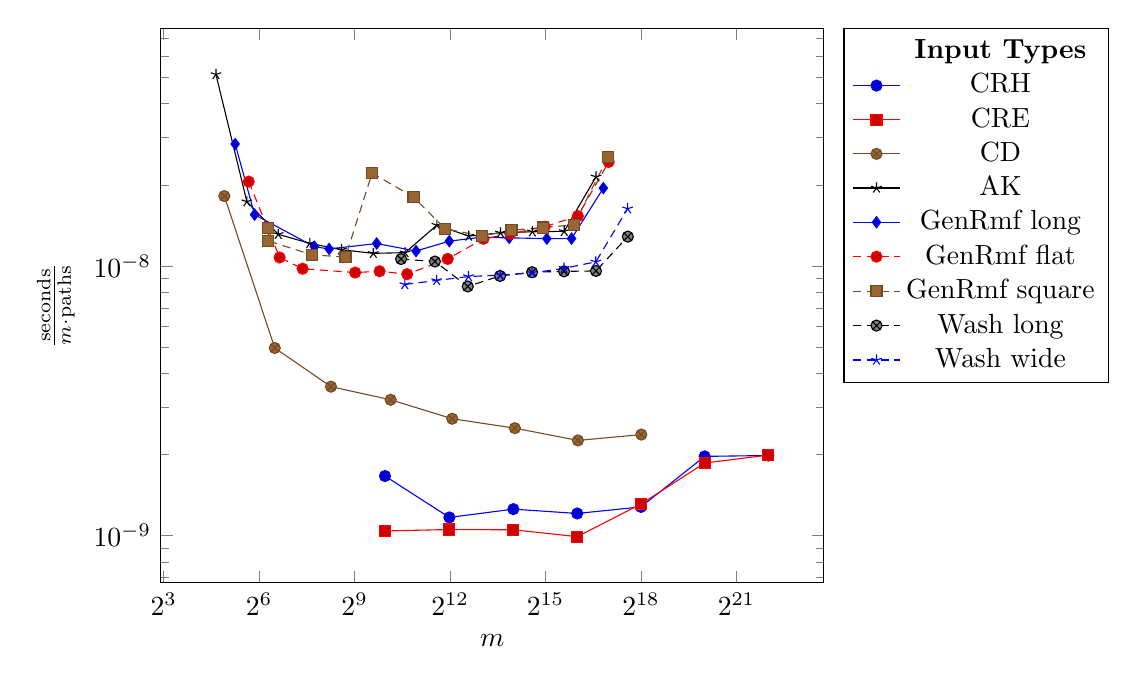
\begin{tikzpicture}
\begin{axis}[
    xlabel=$m$,ylabel=$\frac{\text{seconds}}{m\cdot \text{paths}}$,
    xmode=log,ymode=log,
    log basis x={2},
    legend style=
    {
        legend pos=outer north east
    },
    width=10cm
]
\addlegendimage{legend image code/.code=}
\legend{\textbf{Input Types}, CRH, CRE, CD, AK, GenRmf long, GenRmf flat, GenRmf square, Wash long, Wash wide}
\addplot table[x=n,y=value] {%CRH
n value
992	1.66466E-09
4032	1.16903E-09
16256	1.25451E-09
65280	1.2091E-09
261632	1.27864E-09
1047552	1.96903E-09
4192256	1.98336E-09
};
\addplot table[x=n,y=value] {%CRE
n value
992	1.0413E-09
4032	1.05426E-09
16256	1.05184E-09
65280	9.92107E-10
261632	1.31012E-09
1047552	1.85996E-09
4192256	1.99021E-09
};
\addplot table[x=n,y=value] {%CD
n value
30	1.81717E-08
90	4.96716E-09
306	3.57009E-09
1122	3.19207E-09
4290	2.71479E-09
16770	2.50517E-09
66306	2.25596E-09
263682	2.37129E-09
};
\addplot table[x=n,y=value] {%AK
n value
25	5.13295E-08
49	1.73307E-08
97	1.31136E-08
193	1.21362E-08
385	1.14906E-08
769	1.11464E-08
1537	1.12091E-08
3073	1.41778E-08
6145	1.29195E-08
12289	1.32742E-08
24577	1.34015E-08
49153	1.34511E-08
98305	2.14221E-08
};
\addplot table[x=n,y=value] {%GenRmf long
n value
38	2.83468E-08
58	1.55086E-08
213	1.17957E-08
294	1.15719E-08
828	1.21194E-08
1950	1.13672E-08
4026	1.23664E-08
7868	1.27728E-08
14840	1.27225E-08
33660	1.26353E-08
57717	1.26436E-08
115284	1.94512E-08
};
\addplot table[x=n,y=value] {%GenRmf flat
n value
51	2.05647E-08
100	1.07579E-08
165	9.77235E-09
518	9.45758E-09
882	9.56565E-09
1608	9.32887E-09
3888	1.0626E-08
8484	1.26209E-08
15232	1.31695E-08
32153	1.39854E-08
66150	1.53185E-08
129472	2.43192E-08
};
\addplot table[x=n,y=value] {%GenRmf square
n value
78	1.38184E-08
78	1.23946E-08
204	1.09934E-08
420	1.08071E-08
750	2.21376E-08
1848	1.80034E-08
3690	1.37307E-08
8268	1.29187E-08
15600	1.35717E-08
30780	1.38904E-08
60600	1.42187E-08
127968	2.5442E-08
};
\addplot table[x=n,y=value] {%Wash long
n value
1408	1.06141E-08
2944	1.03926E-08
6016	8.40057E-09
12160	9.18783E-09
24448	9.48726E-09
49024	9.55599E-09
98176	9.58903E-09
196480	1.28548E-08
};
\addplot table[x=n,y=value] {%Wash wide
n value
1528	8.54169E-09
3056	8.84407E-09
6112	9.14132E-09
12224	9.25413E-09
24448	9.42574E-09
48896	9.81213E-09
97792	1.03599E-08
195584	1.63099E-08
};
\end{axis}
\end{tikzpicture}
\caption{Edmonds and Karp performance per $m$ and the number of augmenting paths}
\label{fig:EK_runningTimeappendix}
\end{figure}



\begin{figure}[h]
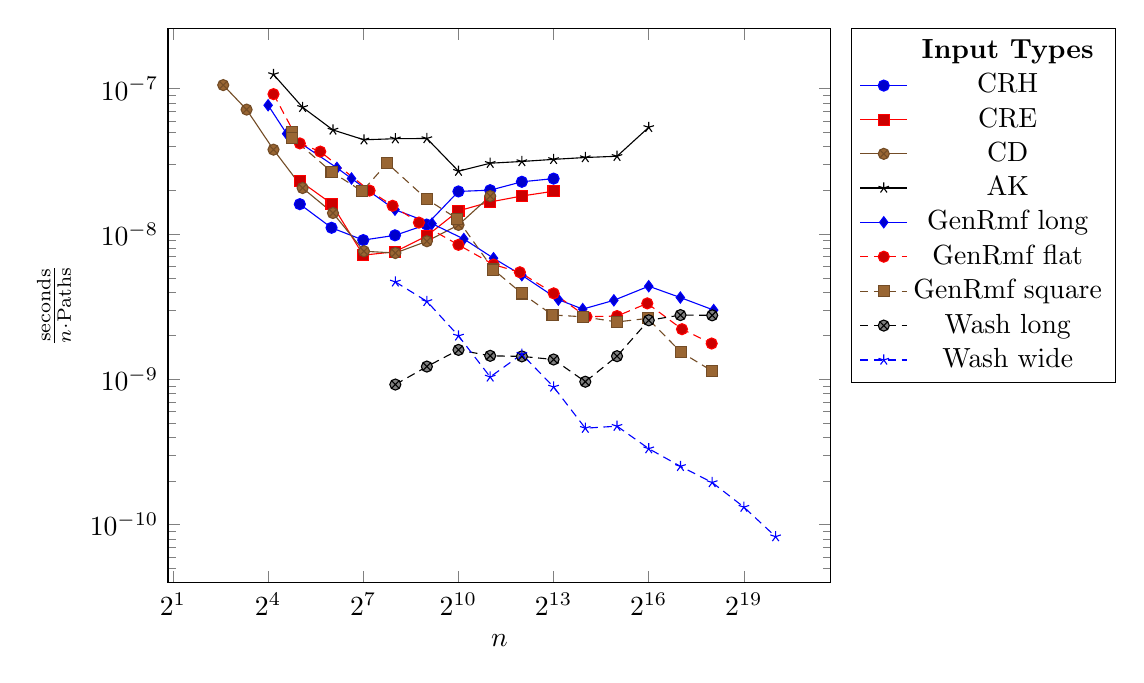
\begin{tikzpicture}
\begin{axis}[
    xlabel=$n$,ylabel=$\frac{\text{seconds}}{n\cdot \text{Paths}}$,
    xmode=log,ymode=log,
    log basis x={2},
    legend style=
    {
        legend pos=outer north east
    },
    width=10cm
]
\addlegendimage{legend image code/.code=}
\legend{\textbf{Input Types}, CRH, CRE, CD, AK, GenRmf long, GenRmf flat, GenRmf square, Wash long, Wash wide}
\addplot table[x=n,y=value] {%CRH
n value
32	1.60662E-08
64	1.10524E-08
128	9.09034E-09
256	9.8052E-09
512	1.16228E-08
1024	1.96589E-08
2048	2.00461E-08
4096	2.29003E-08
8192	2.40805E-08
};
\addplot table[x=n,y=value] {%CRE
n value
32	2.32243E-08
64	1.61998E-08
128	7.16023E-09
256	7.55879E-09
512	9.70943E-09
1024	1.44429E-08
2048	1.66357E-08
4096	1.82794E-08
8192	1.97247E-08
};
\addplot table[x=n,y=value] {%CD
n value
6	1.06002E-07
10	7.18898E-08
18	3.81028E-08
34	2.07454E-08
66	1.39579E-08
130	7.62282E-09
258	7.40559E-09
514	8.92618E-09
1026	1.1564E-08
2050	1.82553E-08
};
\addplot table[x=n,y=value] {%AK
n value
18	1.25445E-07
34	7.45452E-08
66	5.20575E-08
130	4.45512E-08
258	4.5328E-08
514	4.54889E-08
1026	2.71015E-08
2050	3.07429E-08
4098	3.15994E-08
8194	3.2674E-08
16386	3.36491E-08
32770	3.43191E-08
65538	5.42947E-08
};
\addplot table[x=n,y=value] {%GenRmf long
n value
16	7.70404E-08
24	4.90468E-08
72	2.85335E-08
99	2.41266E-08
256	1.47136E-08
575	1.17925E-08
1152	9.25426E-09
2205	6.82108E-09
4096	5.21221E-09
9100	3.54137E-09
15488	3.04506E-09
30589	3.50078E-09
65536	4.37844E-09
130682	3.65803E-09
270848	2.99932E-09
};
\addplot table[x=n,y=value] {%GenRmf flat
n value
18	9.18556E-08
32	4.20773E-08
50	3.69572E-08
147	1.99257E-08
243	1.5665E-08
432	1.19976E-08
1024	8.43176E-09
2205	6.16549E-09
3920	5.46192E-09
8214	3.90928E-09
16807	2.70144E-09
32768	2.72785E-09
63504	3.33529E-09
135531	2.21539E-09
259308	1.76556E-09
};
\addplot table[x=n,y=value] {%GenRmf square
n value
27	5.01265E-08
27	4.60135E-08
64	2.68313E-08
125	1.97155E-08
216	3.07307E-08
512	1.74072E-08
1000	1.27292E-08
2197	5.6998E-09
4096	3.90324E-09
8000	2.77607E-09
15625	2.69714E-09
32768	2.48514E-09
64000	2.62866E-09
132651	1.5397E-09
262144	1.14193E-09
};
\addplot table[x=n,y=value] {%Wash long
n value
258	9.21744E-10
514	1.22555E-09
1026	1.59596E-09
2050	1.45298E-09
4098	1.44002E-09
8194	1.37073E-09
16386	9.63818E-10
32770	1.4445E-09
65538	2.55088E-09
131074	2.77054E-09
262146	2.75927E-09
};
\addplot table[x=n,y=value] {%Wash wide
n value
258	4.6875E-09
514	3.44298E-09
1026	1.9923E-09
2050	1.03997E-09
4098	1.49151E-09
8194	8.8731E-10
16386	4.61535E-10
32770	4.76501E-10
65538	3.33716E-10
131074	2.52127E-10
262146	1.95298E-10
524290	1.32129E-10
1048578	8.27744E-11
};
\end{axis}
\end{tikzpicture}
\caption{Dinic performance per $nP$}
\label{fig:Dinic_runningTimeAppendix}
\end{figure}


\begin{figure}[h]
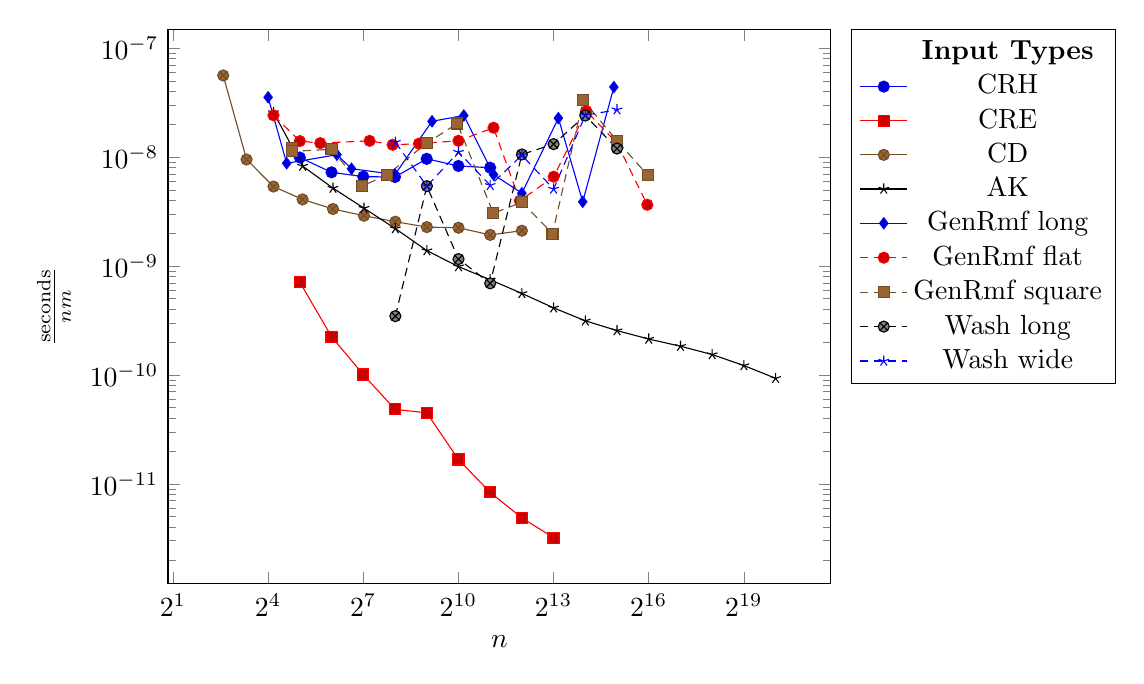
\begin{tikzpicture}
\begin{axis}[
    xlabel=$n$,ylabel=$\frac{\text{seconds}}{nm}$,
    xmode=log,ymode=log,
    log basis x={2},
    legend style=
    {
        legend pos=outer north east
    },
    width=10cm
]
\addlegendimage{legend image code/.code=}
\legend{\textbf{Input Types}, CRH, CRE, CD, AK, GenRmf long, GenRmf flat, GenRmf square, Wash long, Wash wide}
\addplot table[x=n,y=value] {%CRH
n value
32	9.90712E-09
64	7.24742E-09
128	6.61376E-09
256	6.56429E-09
512	9.63395E-09
1024	8.2859E-09
2048	7.99078E-09
};
\addplot table[x=n,y=value] {%CRE
n value
32	7.1015E-10
64	2.24209E-10
128	1.00655E-10
256	4.82229E-11
512	4.48739E-11
1024	1.67318E-11
2048	8.34562E-12
4096	4.86383E-12
8192	3.20329E-12
};
\addplot table[x=n,y=value] {%CD
n value
6	5.61416E-08
10	9.50089E-09
18	5.36295E-09
34	4.08415E-09
66	3.33572E-09
130	2.89291E-09
258	2.55076E-09
514	2.27462E-09
1026	2.24389E-09
2050	1.92973E-09
4098	2.10844E-09
};
\addplot table[x=n,y=value] {%AK
n value
18	2.56647E-08
34	8.26537E-09
66	5.18647E-09
130	3.39477E-09
258	2.20466E-09
514	1.38395E-09
1026	9.86652E-10
2050	7.47385E-10
4098	5.60005E-10
8194	4.12565E-10
16386	3.13874E-10
32770	2.54984E-10
65538	2.13448E-10
131074	1.83323E-10
262146	1.53786E-10
524290	1.21857E-10
1048578	9.30332E-11
};
\addplot table[x=n,y=value] {%GenRmf long
n value
16	3.54335E-08
24	8.77545E-09
72	1.05068E-08
99	7.81762E-09
256	6.92696E-09
575	2.13165E-08
1152	2.40867E-08
2205	6.90549E-09
4096	4.66368E-09
9100	2.27639E-08
15488	3.88656E-09
30589	4.39229E-08
};
\addplot table[x=n,y=value] {%GenRmf flat
n value
18	2.41938E-08
32	1.402E-08
50	1.34336E-08
147	1.40864E-08
243	1.29601E-08
432	1.32838E-08
1024	1.41106E-08
2205	1.8587E-08
3920	3.968E-09
8214	6.60992E-09
16807	2.63829E-08
32768	1.34006E-08
63504	3.647E-09
};
\addplot table[x=n,y=value] {%GenRmf square
n value
27	1.20752E-08
27	1.12842E-08
64	1.17888E-08
125	5.41498E-09
216	6.87753E-09
512	1.34166E-08
1000	2.0345E-08
2197	3.04784E-09
4096	3.8493E-09
8000	1.98347E-09
15625	3.31797E-08
32768	1.41112E-08
64000	6.83458E-09
};
\addplot table[x=n,y=value] {%Wash long
n value
258	3.46356E-10
514	5.40945E-09
1026	1.15649E-09
2050	6.92953E-10
4098	1.05799E-08
8194	1.31438E-08
16386	2.40597E-08
32770	1.19685E-08
};
\addplot table[x=n,y=value] {%Wash wide
n value
258	1.36924E-08
514	5.40668E-09
1026	1.11032E-08
2050	5.50623E-09
4098	1.03918E-08
8194	5.09109E-09
16386	2.41668E-08
32770	2.72197E-08
};
\end{axis}
\end{tikzpicture}
\caption{GT performance per $nm$}
\label{fig:GT_runningTimeAppendix}
\end{figure}



\begin{figure}[h]
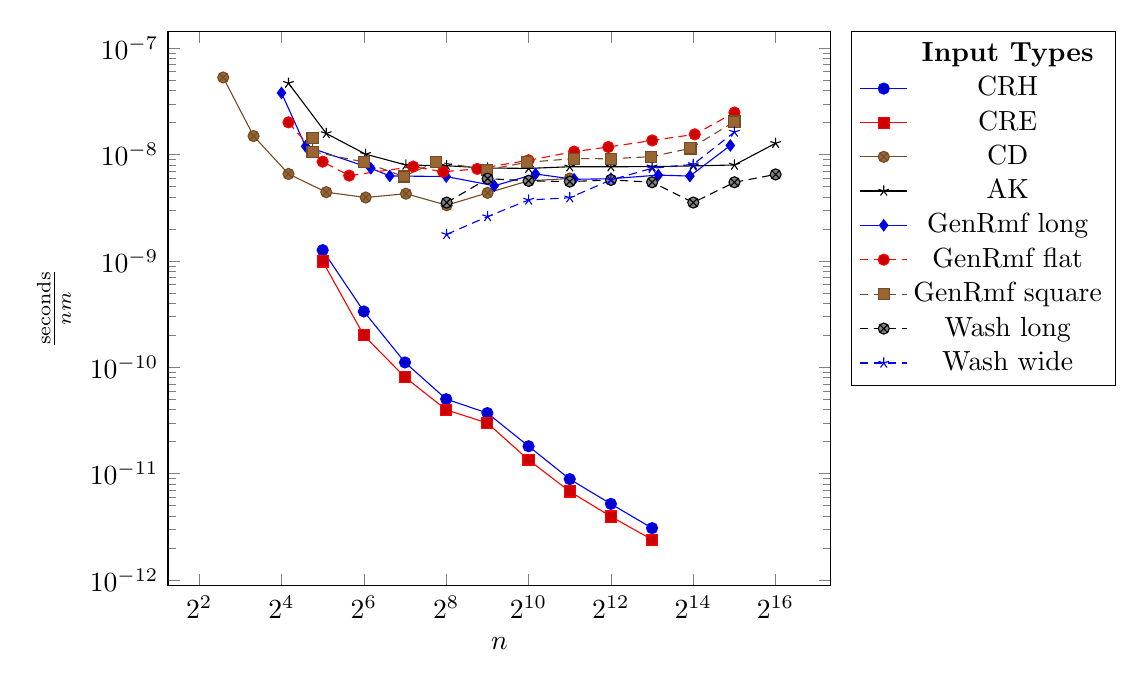
\begin{tikzpicture}
\begin{axis}[
    xlabel=$n$,ylabel=$\frac{\text{seconds}}{nm}$,
    xmode=log,ymode=log,
    log basis x={2},
    legend style=
    {
        legend pos=outer north east
    },
    width=10cm
]
\addlegendimage{legend image code/.code=}
\legend{\textbf{Input Types}, CRH, CRE, CD, AK, GenRmf long, GenRmf flat, GenRmf square, Wash long, Wash wide}
\addplot table[x=n,y=value] {%CRH
n value
32	1.26288E-09
64	3.35238E-10
128	1.11168E-10
256	5.03027E-11
512	3.71824E-11
1024	1.81421E-11
2048	8.90429E-12
4096	5.20555E-12
8192	3.0819E-12
};
\addplot table[x=n,y=value] {%CRE
n value
32	9.90013E-10
64	1.9968E-10
128	8.07477E-11
256	3.98834E-11
512	2.99502E-11
1024	1.35027E-11
2048	6.81994E-12
4096	3.96241E-12
8192	2.40243E-12
};
\addplot table[x=n,y=value] {%CD
n value
6	5.30569E-08
10	1.49299E-08
18	6.57264E-09
34	4.43056E-09
66	3.94952E-09
130	4.2887E-09
258	3.3403E-09
514	4.36561E-09
1026	5.66833E-09
2050	5.95279E-09
};
\addplot table[x=n,y=value] {%AK
n value
18	4.68876E-08
34	1.57975E-08
66	1.0078E-08
130	7.98015E-09
258	7.84601E-09
514	7.4766E-09
1026	7.41183E-09
2050	7.68286E-09
4098	7.68821E-09
8194	7.69572E-09
16386	7.82987E-09
32770	7.98256E-09
65538	1.27783E-08
};
\addplot table[x=n,y=value] {%GenRmf long
n value
16	3.79906E-08
24	1.19665E-08
72	7.4366E-09
99	6.29532E-09
256	6.21655E-09
575	5.09247E-09
1152	6.56912E-09
2205	5.85557E-09
4096	5.92566E-09
9100	6.41111E-09
15488	6.27912E-09
30589	1.21796E-08
};
\addplot table[x=n,y=value] {%GenRmf flat
n value
18	2.00808E-08
32	8.57161E-09
50	6.33991E-09
147	7.7075E-09
243	6.89168E-09
432	7.32937E-09
1024	8.83296E-09
2205	1.06628E-08
3920	1.1773E-08
8214	1.3578E-08
16807	1.54848E-08
32768	2.48237E-08
};
\addplot table[x=n,y=value] {%GenRmf square
n value
27	1.43953E-08
27	1.06515E-08
64	8.51412E-09
125	6.22088E-09
216	8.53572E-09
512	7.21217E-09
1000	8.45903E-09
2197	9.16498E-09
4096	9.1337E-09
8000	9.54867E-09
15625	1.14186E-08
32768	2.04167E-08
};
\addplot table[x=n,y=value] {%Wash long
n value
258	3.53846E-09
514	5.93937E-09
1026	5.66374E-09
2050	5.56832E-09
4098	5.78294E-09
8194	5.49482E-09
16386	3.53918E-09
32770	5.49036E-09
65538	6.50731E-09
};
\addplot table[x=n,y=value] {%Wash wide
n value
258	1.77663E-09
514	2.61444E-09
1026	3.74229E-09
2050	3.93122E-09
4098	5.77718E-09
8194	7.43357E-09
16386	8.0869E-09
32770	1.62903E-08
};
\end{axis}
\end{tikzpicture}
\caption{GT GRC performance per $nm$}
\label{fig:GT_GRC_runningTimeAppendix}
\end{figure}



\begin{figure}[h]
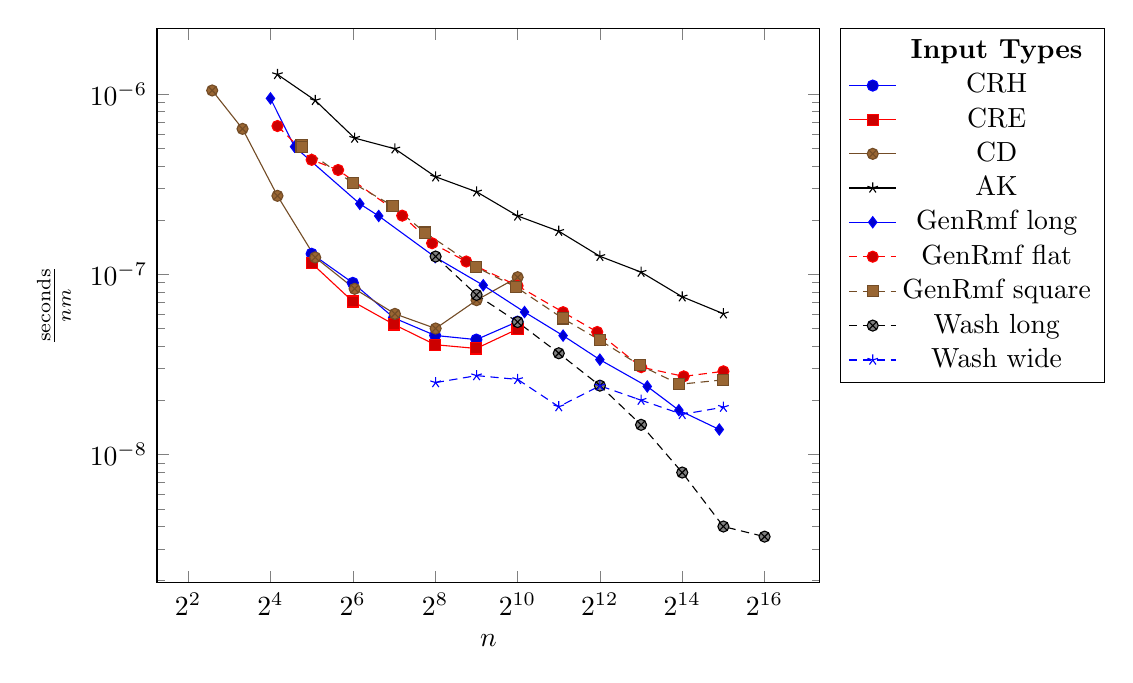
\begin{tikzpicture}
\begin{axis}[
    xlabel=$n$,ylabel=$\frac{\text{seconds}}{nm}$,
    xmode=log,ymode=log,
    log basis x={2},
    legend style=
    {
        legend pos=outer north east
    },
    width=10cm
]
\addlegendimage{legend image code/.code=}
\legend{\textbf{Input Types}, CRH, CRE, CD, AK, GenRmf long, GenRmf flat, GenRmf square, Wash long, Wash wide}
\addplot table[x=n,y=value] {%CRH
n value
32	1.30007E-07
64	8.96393E-08
128	5.72588E-08
256	4.57896E-08
512	4.343E-08
1024	5.46341E-08
};
\addplot table[x=n,y=value] {%CRE
n value
32	1.15261E-07
64	7.06504E-08
128	5.26847E-08
256	4.06767E-08
512	3.87895E-08
1024	4.96835E-08
};
\addplot table[x=n,y=value] {%CD
n value
6	1.04695E-06
10	6.41125E-07
18	2.72502E-07
34	1.24094E-07
66	8.30602E-08
130	6.03361E-08
258	5.00513E-08
514	7.18575E-08
1026	9.63497E-08
};
\addplot table[x=n,y=value] {%AK
n value
18	1.28447E-06
34	9.22187E-07
66	5.69731E-07
130	4.97013E-07
258	3.47541E-07
514	2.8686E-07
1026	2.10738E-07
2050	1.73426E-07
4098	1.25893E-07
8194	1.0284E-07
16386	7.50472E-08
32770	6.04413E-08
};
\addplot table[x=n,y=value] {%GenRmf long
n value
16	9.46111E-07
24	5.10492E-07
72	2.45994E-07
99	2.1071E-07
256	1.24506E-07
575	8.69615E-08
1152	6.17645E-08
2205	4.56919E-08
4096	3.36001E-08
9100	2.38667E-08
15488	1.76328E-08
30589	1.37729E-08
};
\addplot table[x=n,y=value] {%GenRmf flat
n value
18	6.64723E-07
32	4.31634E-07
50	3.79102E-07
147	2.11565E-07
243	1.48769E-07
432	1.17769E-07
1024	8.63694E-08
2205	6.16427E-08
3920	4.78561E-08
8214	3.05494E-08
16807	2.71511E-08
32768	2.89605E-08
};
\addplot table[x=n,y=value] {%GenRmf square
n value
27	5.215E-07
27	5.08105E-07
64	3.20687E-07
125	2.39996E-07
216	1.7053E-07
512	1.09497E-07
1000	8.49219E-08
2197	5.68963E-08
4096	4.30881E-08
8000	3.13326E-08
15625	2.45354E-08
32768	2.59762E-08
};
\addplot table[x=n,y=value] {%Wash long
n value
258	1.25491E-07
514	7.69137E-08
1026	5.43358E-08
2050	3.6474E-08
4098	2.41164E-08
8194	1.46208E-08
16386	7.95112E-09
32770	3.98875E-09
65538	3.50499E-09
};
\addplot table[x=n,y=value] {%Wash wide
n value
258	2.5073E-08
514	2.74194E-08
1026	2.6114E-08
2050	1.84365E-08
4098	2.40671E-08
8194	2.00366E-08
16386	1.6713E-08
32770	1.83213E-08
};
\end{axis}
\end{tikzpicture}
\caption{GR performance per $nm$}
\label{fig:GR_runningTimeAppendix}
\end{figure}

\end{subappendices}

\end{document}
